\documentclass[a4paper,11pt]{report}
\usepackage{float}
\usepackage{thesis}
\usepackage{cite, array, amsmath, url, amsfonts} 
\usepackage{pgfplots}
\usepackage{pgfplotstable}
\usepgfplotslibrary{patchplots,colormaps,statistics,external}
\usepackage{subfigure}


\usetikzlibrary{
	pgfplots.colorbrewer,
}

\newcolumntype{C}[1]{>{\centering\arraybackslash}p{#1}}
\pgfplotsset{compat = newest,
	every axis/.append style={
		scaled ticks=false,
		tick label style={/pgf/number format/fixed, scale=0.7},
		scale only axis,
		smooth,
		width=0.5\textwidth,
		mark repeat=2,
		mark size=1.5pt,
		only marks,
		cycle list/Dark2,
		grid=both,
		label style = {scale=0.7},%
	},
	/tikz/every picture/.append style={
		trim axis left,
		trim axis right,
	},
% define a `cycle list' for marker
cycle list/.define={my marks}{
	every mark/.append style={solid,fill=\pgfkeysvalueof{/pgfplots/mark list fill}},mark=otimes*\\
	every mark/.append style={dashed,fill=\pgfkeysvalueof{/pgfplots/mark list fill}},mark=square*\\
	every mark/.append style={densely dotted,fill=\pgfkeysvalueof{/pgfplots/mark list fill}},mark=triangle*\\
	every mark/.append style={solid,fill=\pgfkeysvalueof{/pgfplots/mark list fill}},mark=diamond*\\
	every mark/.append style={solid,fill=\pgfkeysvalueof{/pgfplots/mark list fill}},mark=square\\
},
}
\pgfplotstableset{
	col sep = comma,
}
%\pgfplotsset{compat = 1.12}
\usepackage[%
font={small,sf},
labelfont=bf,
format=hang,
]{caption}
% The value for \thesistitle should be the title of the thesis in a single line.
\renewcommand{\thesistitle}{
Study of Neural network internals
}

% The value for \authorname should be the name of the student as per the
% administrative records. Add your roll number here within paranthesis.
\renewcommand{\authorname}{Gaurav Kumar Jain}
\renewcommand{\rollnumber}{EMT2013007}
% The value for \mydegree should be 
% 1: for M.Tech., 
% 2: for M.S. by research,
% 3: for Ph.D.
\renewcommand{\mydegree}{1} 

% Values for the date that should go to your title page and certificate page,
% specifically the day, month, and year. 
% Note: Ensure that the date that is used is a valid date. 
%
% \myyear should be year in 4-digit format. 
% \mymonth is the number corresponding to the month, e.g. 1, 2, ..., 12 for 
%          January, February, ..., December, respectively.
% \myday is the number for the day from 1 to 31, depending on the allowable 
%          number of days for the month and year specified in \mymonth and 
%          \myyear.
\renewcommand{\myday}{30}
\renewcommand{\mymonth}{12}
\renewcommand{\myyear}{2016}

% The value for \advisorname should be the name of the advisor without any
% title 
\renewcommand{\advisorname}{Prof. G.Srinivasaraghavan}

% The value for \coadvisorname should be the name of the co-advisor without 
% any title. Use the next line if no co-advisor; otherwise comment 
% out the next line and uncomment the succeeding line. Change the value of 
% \numberofcoadvisors to 1 if there is a coadvisor.
%% \renewcommand{\numberofcoadvisors}{1}
%% \renewcommand{\coadvisorname}{Jane Doe}

% Customize your dedication
\renewcommand{\mydedication}{Dedicated to \\ My parents, My Wife Divya and My sweet daughter Samartha}
\setlength{\parskip}{11pt plus 1pt minus 1pt} 


\tikzexternalize%
\tikzsetexternalprefix{Images/}%
%\tikzset{external/force remake}



\begin{document}

\maketitlepages
\setchapterindexing


% chap1.tex

\chapter{Introduction and Overview}\label{chap:intro}
\noindent Deep neural networks have demonstrated excellent results in many machine learning tasks [REFERENCES:TBD] and became a default choice for machine learning researchers irrespective of the end result they achieved.
Computer vision , Natural language and Speech processing tasks have scaled to the next level of accuracies using these networks.
\paragraph{Structure:} The core structure of Neural network is the Neurons arranged in a layer manner also known as hidden layer and stack of these layers with interconnected Neurons provides depth to the network. This arrangement of layers is known as network architecture. A simple Neural Network is shown in Figure~\ref{fig:nn_simple_dep}.
Several networks are proposed till date for the range of machine learning tasks.[REFERENCES:TBD]
\paragraph{Training:} Network architecture remains passive till it is trained and parameters of the networks are estimated for the desired level of prediction performance on data samples outside training data set, also known as Generalization performance.
The most important part is the training strategy which encompass choosing the hyper-parameters to intermediate updates along with learning algorithm.
The number of hyper-parameters termed as annoying knobs to be adjusted [Bengio 2012: Practical recommendations] and famously known as nuisance parameters are quite high. On top of this range of choices for these hyper-parameters make exhaustive search impractical.
Once these parameters are chosen, training can be proceed and the algorithm, which is more often than not is Stochastic gradient descent [References] along with Back propagation [Reference: Rumelhart] as a default choice allows network to evolve from untrained to train network.Training stops as per stopping criterion.

\begin{figure}
	\centering
	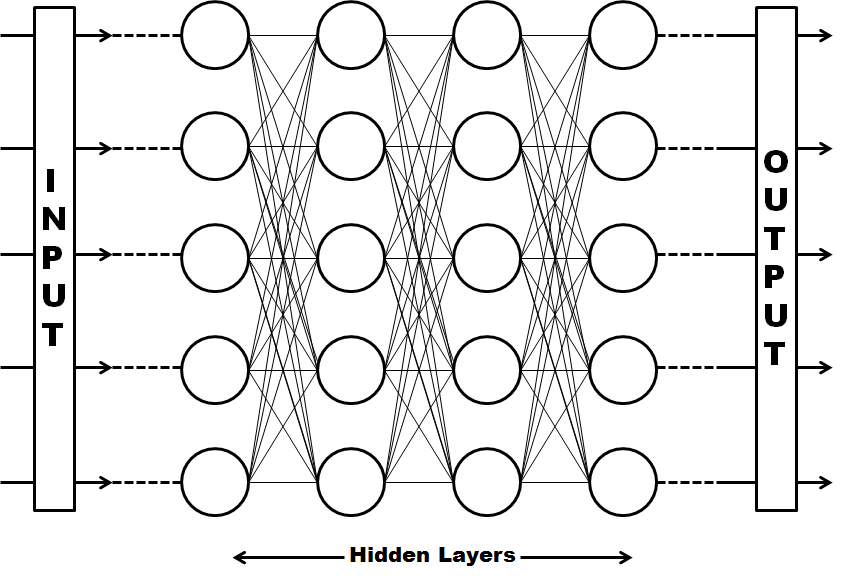
\includegraphics[scale=0.60]{Images/nn_simple_dep}
	\caption{\label{fig:nn_simple_dep} A Simple Neural Network} 
\end{figure}


Considering all these background the \textbf{Training Life Cycle} of DNN's has 3 main stages as shown in Figure~\ref{fig:dnn_lifecycle}

\begin{enumerate}
	\item Choosing network structure
	\item Selection of hyper parameters and training algorithm
	\item Network updates during training and stopping criterion
\end{enumerate}

\begin{figure}
	\centering
	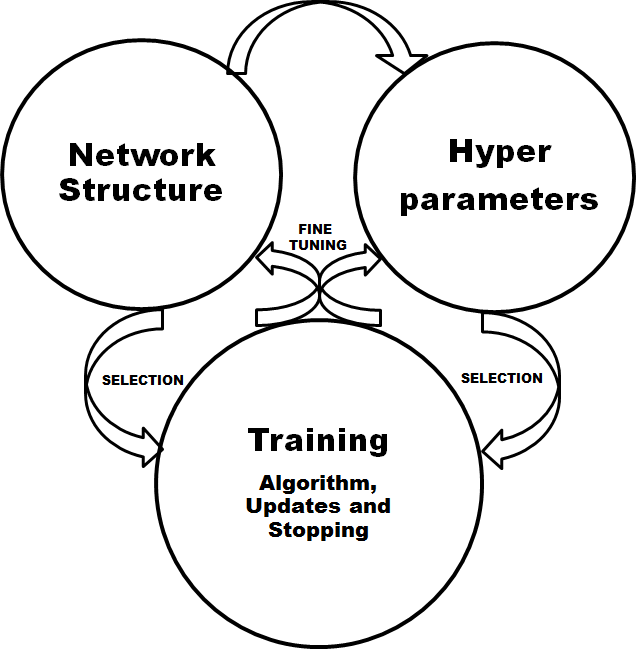
\includegraphics[scale=0.60]{Images/dnn_training_lifecycle}
	\caption{\label{fig:dnn_lifecycle} DNN Training Lifecycle} 
\end{figure}
\section{Chapters Organization}
This study is divided into 6 chapters, Chapter 2, discusses \textbf{Network architecture}, Chapter 3 discusses \textbf{Hyper-parameters}, Chapter 4 discusses \textbf{Training the Network}, Chapter 5 discusses the \textbf{Insights and Recommendations} from this study. Chapter 6 \textbf{concludes} and poses some \textbf{open questions} for future work.

\subsection{Network types}
Chapter \ref{chap:nwstruct} details different architectures, which can be seen as small survey on the state of the art networks used in deep learning.We will keep them for study purposes.

As we studied the details and interdependencies among the training parameters,so we have used our own network, we call it \textbf{ GsNet}. We recommend to use them for comparative study of this kind.
Table \ref{tab:gsnet} shows the layers configuration of GsNet-2,GsNet-3 and GsNet-5.
\begin{table}[!htbp]
	\centering
	\caption{\textbf{GsNet architectures}}
	\label{tab:gsnet}
	\vspace{2mm}
	\begin{tabular}{|l|l|l|}
		\hline
		\hline
		\textbf{GsNet-2} & \textbf{GsNet-3} & \textbf{GsNet-5} 		\\
		\hline
		\hline
		conv 3x3x64 & conv 3x3x64 	& conv 3x3x64 		\\
		pool 2x2    & pool 2x2 		& pool 2x2			\\
		\hline 
		conv 3x3x64 & conv 3x3x64 	& conv 3x3x64 		\\
		pool 2x2    & pool 2x2 		& pool 2x2 			\\
		\hline
		
		& conv 3x3x64 	& conv 3x3x64 		\\
		& pool 2x2 		& pool 2x2 			\\
		\hline
		&        		& conv 3x3x64 		\\
		&  				& pool 2x2 			\\
		\hline
		&  				& conv 3x3x64 		\\
		&  				& pool 2x2 			\\
		\hline
		dense,128 	& dense,128 	& dense,128  		\\
		\hline
		softmax,c 	& softmax,c 	& softmax,c  		\\
		\hline
		\hline
	\end{tabular}
\end{table}

We have used these networks for our experiments and their analysis. This may bring how depth affects learning. Different architectures in practice are described, which can be seen as small survey on state of the art network architectures in chapter \ref{chap:nwstruct}.

\subsection{Hyper-parameters}
Hyper-parameters are discussed in chapter \ref{chap:hyperparams}.Main parameters, which we studied are as following
\begin{enumerate}
	\item Batch Size
	\item Optimizations
	\item Initializations
\end{enumerate} 

Firstly we describe all the different prescribed available techniques for these parameters which can be seen as a small survey of the available studies, experimental results and techniques.

Secondly we present results of almost exhaustive set of parameters configuration. Then best of parameters and configurations are chosen for the next set of experiments.

\subsection{Training the network}

Chapter \ref{chap:training} discusses training the network and study which describes different techniques used in training.We will also explain our training set up which is used for our experiments.


\subsection{Insights and Recommendations}
Chapter \ref{chap:recommendations} provides all insights and analysis of our results. This includes well performing strategies as well as strategies which may didn't  perform well.
Based on these we will describe our recommendations. Also we will explain novel technique which perform well and provide more stability to the learning system.

\subsection{Conclusion}
Chapter \ref{chap:conclusions} concludes with the summary of our study and future direction of this work.

%\iffalse
\section{Notations used}
This section explains the notations used through out this study.
\subsection{DNN Setting}
DNN goal is to approximate a target function $g^*$ for the unknown distribution input $X^*=(x_1,x_2,......x_d)^T \in \mathbb{R}^d$. The target value is $Y^*=(y_1,y_2,........y_s) \in \mathbb{R}^s$. if $\theta^*$ is the parameters associated, then 
\begin{equation}
Y^*=g^*(X^*, \theta^*)
\end{equation}								

$X^*$ represents entire input data for the underlying input distribution. 
Getting $X^*$ is almost impossible, so generally $g^*$ is approximate using the representative input $X$ of size $N$ which is sampled from $X^*$ and hoped to have same distribution as the original input distribution. Let $Y$ is the target value for $X$.

So DNN problem reduces to approximating $ g^*$ using $(X,Y)$ of size $N$. $\theta=(\theta_1,\theta_2...\theta_m) \in \mathbb{R}^m$ represents the parameters which gives best approximation for target function. Finally the DNN has to learn the best $\theta$  such that $g(X,\theta) \sim g^*$. 

$g$ represents a chained function in context of DNN as it flows from input to output via hidden layers as shown in \ref{fig:nn_simple_dep}. $g$ as chained function flowing via hidden layers can  be written as
\begin{equation}
g(X)=g^K(g^{K-1}(g^{K-2}......(g^2(g^1(X))).......)) 
\end{equation}
where $K$ represents total number of hidden layers and $\{g^k, k=1....K\}$ is output of $k^{th}$ layer.Let $\hat{Y}=g(X)$ then lets define a loss function $\mathcal{L}(\hat{Y},Y)$ as the cost it incurs using $g(X)$ to approximate $g^*(X)$ and hence it is also known as cost function.

The gradient of $\mathcal{L}$ with respect to $\theta$ is denoted as $\nabla_{\theta_{t}}\mathcal{L}(\theta_{t})$ at $t^{th}$ iteration. For simplicity we denote this as $\nabla_{\theta_{t}}$, where $\theta_{t}$ denotes the network parameters at iteration/time $t$.

\paragraph{Network Parameters}
%\fi
%\section{Results}
First we will see results related to different database and parameters configurations.
\begin{figure}[H]
	\hspace{-1cm}
	\begin{tabular}{C{.48\textwidth}C{.48\textwidth}}
		%%%%%%%%%%%%%%%%%%%%%% 1 %%%%%%%%%%%%%%%%%%%%%%%%%%%%%%%%%%%
		\subfigure [Training accuracy] {
			\begin{tikzpicture} %
			\begin{axis}[smooth,
			legend pos = south east,
			xlabel={$epochs$}, %
			ylabel={$accuracy$}, %
			mark repeat=10,%
			cycle list/Dark2,
			xticklabel style={/pgf/number format/.cd,fixed,precision=2},%
			%width=0.25
			] %
			\addplot table[x expr=\coordindex , y={acc}, col sep=comma] {Results/cifar100_ThreeLayer_100B_0E_adamax_he_u.csv};
			\addlegendentry{minibatch};%				
			\addplot table[x expr=\coordindex , y={acc}, col sep=comma] {Results/cifar100_carebatch_ThreeLayer_100B_0E_adamax_he_u.csv};
			\addlegendentry{minibatch+care};
			\end{axis} %
			\end{tikzpicture}
		}&
		\subfigure [Validation Accuracy] {
			\begin{tikzpicture} %
			\begin{axis}[smooth,
			legend pos = south east,
			xlabel={$epochs$}, %
			ylabel={$accuracy$}, %
			mark repeat=10,%
			cycle list/Dark2,
			xticklabel style={/pgf/number format/.cd,fixed,precision=2},%
			%width=0.25
			] %
			\addplot table[x expr=\coordindex , y={val_acc}, col sep=comma] {Results/cifar100_ThreeLayer_100B_0E_adamax_he_u.csv};
			\addlegendentry{minibatch};%				
			\addplot table[x expr=\coordindex , y={val_acc}, col sep=comma] {Results/cifar100_carebatch_ThreeLayer_100B_0E_adamax_he_u.csv};
			\addlegendentry{minibatch+care};
			\end{axis} %
			\end{tikzpicture}
		} \\
		\subfigure [Training loss] {
			\begin{tikzpicture} %
			\begin{axis}[smooth,
			xlabel={$epochs$}, %
			ylabel={$error$}, %
			mark repeat=10,%
			cycle list/Dark2,
			xticklabel style={/pgf/number format/.cd,fixed,precision=2},
			] %
			\addplot table[x expr=\coordindex , y={loss}, col sep=comma] {Results/cifar100_ThreeLayer_100B_0E_adamax_he_u.csv};
			\addlegendentry{minibatch};%			
			\addplot table[x expr=\coordindex , y={loss}, col sep=comma] {Results/cifar100_carebatch_ThreeLayer_100B_0E_adamax_he_u.csv};
			\addlegendentry{minibatch+care};
			\end{axis} %
			\end{tikzpicture}
		}&
		\subfigure [Validation loss] {
			\begin{tikzpicture} %
			\begin{axis}[smooth,
			xlabel={$epochs$}, %
			ylabel={$error$}, %
			mark repeat=10,%
			cycle list/Dark2,
			xticklabel style={/pgf/number format/.cd,fixed,precision=2},
			] %
			\addplot table[x expr=\coordindex , y={val_loss}, col sep=comma] {Results/cifar100_ThreeLayer_100B_0E_adamax_he_u.csv};
			\addlegendentry{minibatch};%			
			\addplot table[x expr=\coordindex , y={val_loss}, col sep=comma] {Results/cifar100_carebatch_ThreeLayer_100B_0E_adamax_he_u.csv};
			\addlegendentry{minibatch+care};
			\end{axis} %
			\end{tikzpicture}
		}
	\end{tabular}
	\caption {\textit{hessian uniform,batch size=100,three layer}}
\end{figure}

\begin{figure}[H]
	\hspace{-1cm}
	\begin{tabular}{C{.48\textwidth}C{.48\textwidth}}
		%%%%%%%%%%%%%%%%%%%%%% 1 %%%%%%%%%%%%%%%%%%%%%%%%%%%%%%%%%%%
		\subfigure [Training accuracy] {
			\begin{tikzpicture} %
			\begin{axis}[smooth,
			legend pos = south east,
			xlabel={$epochs$}, %
			ylabel={$accuracy$}, %
			mark repeat=10,%
			cycle list/Dark2,
			xticklabel style={/pgf/number format/.cd,fixed,precision=2},%
			%width=0.25
			] %
			\addplot table[x expr=\coordindex , y={acc}, col sep=comma] {Results/cifar100_FiveLayer_100B_0E_adamax_gl_u.csv};
			\addlegendentry{minibatch};%				
			\addplot table[x expr=\coordindex , y={acc}, col sep=comma] {Results/cifar100_carebatch_FiveLayer_100B_0E_adamax_gl_u.csv};
			\addlegendentry{minibatch+care};
			\end{axis} %
			\end{tikzpicture}
		}&
		\subfigure [Validation Accuracy] {
			\begin{tikzpicture} %
			\begin{axis}[smooth,
			legend pos = south east,
			xlabel={$epochs$}, %
			ylabel={$accuracy$}, %
			mark repeat=10,%
			cycle list/Dark2,
			xticklabel style={/pgf/number format/.cd,fixed,precision=2},%
			%width=0.25
			] %
			\addplot table[x expr=\coordindex , y={val_acc}, col sep=comma] {Results/cifar100_FiveLayer_100B_0E_adamax_gl_u.csv};
			\addlegendentry{minibatch};%				
			\addplot table[x expr=\coordindex , y={val_acc}, col sep=comma] {Results/cifar100_carebatch_FiveLayer_100B_0E_adamax_gl_u.csv};
			\addlegendentry{minibatch+care};
			\end{axis} %
			\end{tikzpicture}
		} \\
		\subfigure [Training loss] {
			\begin{tikzpicture} %
			\begin{axis}[smooth,
			xlabel={$epochs$}, %
			ylabel={$error$}, %
			mark repeat=10,%
			cycle list/Dark2,
			xticklabel style={/pgf/number format/.cd,fixed,precision=2},
			] %
			\addplot table[x expr=\coordindex , y={loss}, col sep=comma] {Results/cifar100_FiveLayer_100B_0E_adamax_gl_u.csv};
			\addlegendentry{minibatch};%			
			\addplot table[x expr=\coordindex , y={loss}, col sep=comma] {Results/cifar100_carebatch_FiveLayer_100B_0E_adamax_gl_u.csv};
			\addlegendentry{minibatch+care};
			\end{axis} %
			\end{tikzpicture}
		}&
		\subfigure [Validation loss] {
			\begin{tikzpicture} %
			\begin{axis}[smooth,
			xlabel={$epochs$}, %
			ylabel={$error$}, %
			mark repeat=10,%
			xticklabel style={/pgf/number format/.cd,fixed,precision=2},
			] %
			\addplot table[x expr=\coordindex , y={val_loss}, col sep=comma] {Results/cifar100_FiveLayer_100B_0E_adamax_gl_u.csv};
			\addlegendentry{minibatch};%			
			\addplot table[x expr=\coordindex , y={val_loss}, col sep=comma] {Results/cifar100_carebatch_FiveLayer_100B_0E_adamax_gl_u.csv};
			\addlegendentry{minibatch+care};
			\end{axis} %
			\end{tikzpicture}
		}
	\end{tabular}
	\caption {\textit{glorot uniform,batch size=100,five layer}}
\end{figure}

\begin{figure}[H]
	\hspace{-1cm}
	\begin{tabular}{C{.48\textwidth}C{.48\textwidth}}
		%%%%%%%%%%%%%%%%%%%%%% 1 %%%%%%%%%%%%%%%%%%%%%%%%%%%%%%%%%%%
		\subfigure [Training accuracy] {
			\begin{tikzpicture} %
			\begin{axis}[smooth,
			legend pos = south east,
			xlabel={$epochs$}, %
			ylabel={$accuracy$}, %
			mark repeat=10,%
			xticklabel style={/pgf/number format/.cd,fixed,precision=2},%
			%width=0.25
			] %
			\addplot table[x expr=\coordindex , y={acc}, col sep=comma] {Results/cifar100_ThreeLayer_100B_0E_adamax_gl_u.csv};
			\addlegendentry{minibatch};%				
			\addplot table[x expr=\coordindex , y={acc}, col sep=comma] {Results/cifar100_carebatch_ThreeLayer_100B_0E_adamax_gl_u.csv};
			\addlegendentry{minibatch+care};
			\end{axis} %
			\end{tikzpicture}
		}&
		\subfigure [Validation Accuracy] {
			\begin{tikzpicture} %
			\begin{axis}[smooth,
			legend pos = south east,
			xlabel={$epochs$}, %
			ylabel={$accuracy$}, %
			mark repeat=10,%
			cycle list/Dark2,
			xticklabel style={/pgf/number format/.cd,fixed,precision=2},%
			%width=0.25
			] %
			\addplot table[x expr=\coordindex , y={val_acc}, col sep=comma] {Results/cifar100_ThreeLayer_100B_0E_adamax_gl_u.csv};
			\addlegendentry{minibatch};%				
			\addplot table[x expr=\coordindex , y={val_acc}, col sep=comma] {Results/cifar100_carebatch_ThreeLayer_100B_0E_adamax_gl_u.csv};
			\addlegendentry{minibatch+care};
			\end{axis} %
			\end{tikzpicture}
		} \\
		\subfigure [Training loss] {
			\begin{tikzpicture} %
			\begin{axis}[smooth,
			xlabel={$epochs$}, %
			ylabel={$error$}, %
			mark repeat=10,%
			cycle list/Dark2,
			xticklabel style={/pgf/number format/.cd,fixed,precision=2},
			] %
			\addplot table[x expr=\coordindex , y={loss}, col sep=comma] {Results/cifar100_ThreeLayer_100B_0E_adamax_gl_u.csv};
			\addlegendentry{minibatch};%			
			\addplot table[x expr=\coordindex , y={loss}, col sep=comma] {Results/cifar100_carebatch_ThreeLayer_100B_0E_adamax_gl_u.csv};
			\addlegendentry{minibatch+care};
			\end{axis} %
			\end{tikzpicture}
		}&
		\subfigure [Validation loss] {
			\begin{tikzpicture} %
			\begin{axis}[smooth,
			xlabel={$epochs$}, %
			ylabel={$error$}, %
			mark repeat=10,%
			cycle list/Dark2,
			xticklabel style={/pgf/number format/.cd,fixed,precision=2},
			] %
			\addplot table[x expr=\coordindex , y={val_loss}, col sep=comma] {Results/cifar100_ThreeLayer_100B_0E_adamax_gl_u.csv};
			\addlegendentry{minibatch};%			
			\addplot table[x expr=\coordindex , y={val_loss}, col sep=comma] {Results/cifar100_carebatch_ThreeLayer_100B_0E_adamax_gl_u.csv};
			\addlegendentry{minibatch+care};
			\end{axis} %
			\end{tikzpicture}
		}
	\end{tabular}
	\caption {\textit{glorot uniform,batch size=100,three layer}}
\end{figure}

\begin{figure}[H]
	\hspace{-1cm}
	\begin{tabular}{C{.48\textwidth}C{.48\textwidth}}
		%%%%%%%%%%%%%%%%%%%%%% 1 %%%%%%%%%%%%%%%%%%%%%%%%%%%%%%%%%%%
		\subfigure [Training accuracy] {
			\begin{tikzpicture} %
			\begin{axis}[smooth,
			legend pos = south east,
			xlabel={$epochs$}, %
			ylabel={$accuracy$}, %
			mark repeat=10,%
			cycle list/Dark2,
			xticklabel style={/pgf/number format/.cd,fixed,precision=2},%
			%width=0.25
			] %
			\addplot table[x expr=\coordindex , y={acc}, col sep=comma] {Results/cifar100_FiveLayer_100B_0E_adamax_gl_u.csv};
			\addlegendentry{minibatch};%				
			\addplot table[x expr=\coordindex , y={acc}, col sep=comma] {Results/cifar100_carebatch_FiveLayer_100B_0E_adamax_gl_u.csv};
			\addlegendentry{minibatch+care};
			\end{axis} %
			\end{tikzpicture}
		}&
		\subfigure [Validation Accuracy] {
			\begin{tikzpicture} %
			\begin{axis}[smooth,
			legend pos = south east,
			xlabel={$epochs$}, %
			ylabel={$accuracy$}, %
			mark repeat=10,%
			cycle list/Dark2,
			xticklabel style={/pgf/number format/.cd,fixed,precision=2},%
			%width=0.25
			] %
			\addplot table[x expr=\coordindex , y={val_acc}, col sep=comma] {Results/cifar100_FiveLayer_100B_0E_adamax_gl_u.csv};
			\addlegendentry{minibatch};%				
			\addplot table[x expr=\coordindex , y={val_acc}, col sep=comma] {Results/cifar100_carebatch_FiveLayer_100B_0E_adamax_gl_u.csv};
			\addlegendentry{minibatch+care};
			\end{axis} %
			\end{tikzpicture}
		} \\
		\subfigure [Training loss] {
			\begin{tikzpicture} %
			\begin{axis}[smooth,
			xlabel={$epochs$}, %
			ylabel={$error$}, %
			mark repeat=10,%
			cycle list/Dark2,
			xticklabel style={/pgf/number format/.cd,fixed,precision=2},
			] %
			\addplot table[x expr=\coordindex , y={loss}, col sep=comma] {Results/cifar100_FiveLayer_100B_0E_adamax_gl_u.csv};
			\addlegendentry{minibatch};%			
			\addplot table[x expr=\coordindex , y={loss}, col sep=comma] {Results/cifar100_carebatch_FiveLayer_100B_0E_adamax_gl_u.csv};
			\addlegendentry{minibatch+care};
			\end{axis} %
			\end{tikzpicture}
		}&
		\subfigure [Validation loss] {
			\begin{tikzpicture} %
			\begin{axis}[smooth,
			xlabel={$epochs$}, %
			ylabel={$error$}, %
			mark repeat=10,%
			cycle list/Dark2,
			xticklabel style={/pgf/number format/.cd,fixed,precision=2},
			] %
			\addplot table[x expr=\coordindex , y={val_loss}, col sep=comma] {Results/cifar100_FiveLayer_100B_0E_adamax_gl_u.csv};
			\addlegendentry{minibatch};%			
			\addplot table[x expr=\coordindex , y={val_loss}, col sep=comma] {Results/cifar100_carebatch_FiveLayer_100B_0E_adamax_gl_u.csv};
			\addlegendentry{minibatch+care};
			\end{axis} %
			\end{tikzpicture}
		}
	\end{tabular}
	\caption {\textit{glorot uniform,batch size=100,five layer}}
\end{figure}


	\begin{figure}[H]
		\hspace{-1cm}
		\begin{tabular}{C{.48\textwidth}C{.48\textwidth}}
			%%%%%%%%%%%%%%%%%%%%%% 1 %%%%%%%%%%%%%%%%%%%%%%%%%%%%%%%%%%%
			\subfigure [Training accuracy] {
				\begin{tikzpicture} %
				\begin{axis}[smooth,
				legend pos = south east,
				xlabel={$epochs$}, %
				ylabel={$accuracy$}, %
				mark repeat=10,%
				xticklabel style={/pgf/number format/.cd,fixed,precision=2},
				] %
				\addplot table[x expr=\coordindex , y={acc}, col sep=comma] {Results/cifar100_ThreeLayer_100B_0E_adamax_gl_u.csv};
				\addlegendentry{Three Layer};%				
				\addplot table[x expr=\coordindex , y={acc}, col sep=comma] {Results/cifar100_FiveLayer_100B_0E_adamax_gl_u.csv};
				\addlegendentry{Five Layer};
				\end{axis} %
				\end{tikzpicture}
			}&
			\subfigure [Validation accuracy] {
				\begin{tikzpicture} %
				\begin{axis}[smooth,
				legend pos = south east,
				xlabel={$epochs$}, %
				mark repeat=10,%
				xticklabel style={/pgf/number format/.cd,fixed,precision=2},
				] %
				\addplot table[x expr=\coordindex , y={val_acc}, col sep=comma] {Results/cifar100_ThreeLayer_100B_0E_adamax_gl_u.csv};
				\addlegendentry{Three Layer};%				
				\addplot table[x expr=\coordindex , y={val_acc}, col sep=comma] {Results/cifar100_FiveLayer_100B_0E_adamax_gl_u.csv};
				\addlegendentry{Five Layer};
				\end{axis} %
				\end{tikzpicture}
			} \\
			\subfigure [Training loss] {
				\begin{tikzpicture} %
				\begin{axis}[smooth,
				xlabel={$epochs$}, %
				ylabel={$error$}, %
				mark repeat=10,%
				xticklabel style={/pgf/number format/.cd,fixed,precision=2},
				] %
				\addplot table[x expr=\coordindex , y={loss}, col sep=comma] {Results/cifar100_ThreeLayer_100B_0E_adamax_gl_u.csv};
				\addlegendentry{Three Layer};%				
				\addplot table[x expr=\coordindex , y={loss}, col sep=comma] {Results/cifar100_FiveLayer_100B_0E_adamax_gl_u.csv};
				\addlegendentry{Five Layer};
				\end{axis} %
				\end{tikzpicture}
			}&
			\subfigure [Validation loss] {
				\begin{tikzpicture} %
				\begin{axis}[smooth,
				xlabel={$epochs$}, %
				mark repeat=10,%
				xticklabel style={/pgf/number format/.cd,fixed,precision=2},
				] %
				\addplot table[x expr=\coordindex , y={val_loss}, col sep=comma] {Results/cifar100_ThreeLayer_100B_0E_adamax_gl_u.csv};
				\addlegendentry{Three Layer};%				
				\addplot table[x expr=\coordindex , y={val_loss}, col sep=comma] {Results/cifar100_FiveLayer_100B_0E_adamax_gl_u.csv};
				\addlegendentry{Five Layer};
				\end{axis} %
				\end{tikzpicture}
			}
		\end{tabular}
		\caption {\textit{optimizer=adamax, initializer=glorot uniform and batch size=100}}
	\end{figure}
	
	\begin{figure}[H]
		\hspace{-1cm}
		\begin{tabular}{C{.48\textwidth}C{.48\textwidth}}
			%%%%%%%%%%%%%%%%%%%%%% 1 %%%%%%%%%%%%%%%%%%%%%%%%%%%%%%%%%%%
			\subfigure [Training accuracy] {
				\begin{tikzpicture} %
				\begin{axis}[smooth,
				legend pos = south east,
				xlabel={$epochs$}, %
				ylabel={$accuracy$}, %
				mark repeat=10,%
				cycle list/Dark2,
				xticklabel style={/pgf/number format/.cd,fixed,precision=2},
				] %
				\addplot table[x expr=\coordindex , y={acc}, col sep=comma] {Results/cifar100_ThreeLayer_100B_0E_adamax_he_u.csv};
				\addlegendentry{Three Layer};%				
				\addplot table[x expr=\coordindex , y={acc}, col sep=comma] {Results/cifar100_FiveLayer_100B_0E_adamax_he_u.csv};
				\addlegendentry{Five Layer};
				\end{axis} %
				\end{tikzpicture}
			}&
			\subfigure [Validation accuracy] {
				\begin{tikzpicture} %
				\begin{axis}[smooth,
				legend pos = south east,
				xlabel={$epochs$}, %
				mark repeat=10,%
				cycle list/Dark2,
				xticklabel style={/pgf/number format/.cd,fixed,precision=2},
				] %
				\addplot table[x expr=\coordindex , y={val_acc}, col sep=comma] {Results/cifar100_ThreeLayer_100B_0E_adamax_he_u.csv};
				\addlegendentry{Three Layer};%				
				\addplot table[x expr=\coordindex , y={val_acc}, col sep=comma] {Results/cifar100_FiveLayer_100B_0E_adamax_he_u.csv};
				\addlegendentry{Five Layer};
				\end{axis} %
				\end{tikzpicture}
			} \\
			\subfigure [Training loss] {
				\begin{tikzpicture} %
				\begin{axis}[smooth,
				xlabel={$epochs$}, %
				ylabel={$error$}, %
				%mark repeat=10,%
				cycle list/Dark2,
				xticklabel style={/pgf/number format/.cd,fixed,precision=2},
				] %
				\addplot table[x expr=\coordindex , y={loss}, col sep=comma] {Results/cifar100_ThreeLayer_100B_0E_adamax_gl_u.csv};
				\addlegendentry{Three Layer};%				
				\addplot table[x expr=\coordindex , y={loss}, col sep=comma] {Results/cifar100_FiveLayer_100B_0E_adamax_gl_u.csv};
				\addlegendentry{Five Layer};
				\end{axis} %
				\end{tikzpicture}
			}&
			\subfigure [Validation loss] {
				\begin{tikzpicture} %
				\begin{axis}[smooth,
				xlabel={$epochs$}, %
				mark repeat=10,%
				cycle list/Dark2,
				xticklabel style={/pgf/number format/.cd,fixed,precision=2},
				] %
				\addplot table[x expr=\coordindex , y={val_loss}, col sep=comma] {Results/cifar100_ThreeLayer_100B_0E_adamax_gl_u.csv};
				\addlegendentry{Three Layer};%				
				\addplot table[x expr=\coordindex , y={val_loss}, col sep=comma] {Results/cifar100_FiveLayer_100B_0E_adamax_gl_u.csv};
				\addlegendentry{Five Layer};
				\end{axis} %
				\end{tikzpicture}
			}
		\end{tabular}
		\caption {\textit{optimizer=adamax, initializer=hessian uniform and batch size=100}}
	\end{figure}


%\section{MNIST Results}
First we will see results related to different database and parameters configurations.


\begin{figure}[H]
	\hspace{-1cm}
			\begin{tikzpicture} %
			\begin{axis}[smooth,
			legend pos = north east,
			mark repeat=10,%
			] %
			\addplot3 [surf,z buffer=sort, mesh/rows=5, shader=interp]
			table[y={batch}, x={index} , z={val_loss}, col sep=comma] {ResultsNormal/data.csv};
			\end{axis} %
			\end{tikzpicture}
	\end{figure}


%%%%%%%%%%%%%%%%%%%%%%%%%%%%%%%%%%%%START: BATCH DEPENDENCIES RESULTS%%%%%%%%%%%%%%%%%%%%%%%%%%%%%%%

\begin{figure}[H]
	\hspace{-1cm}
	\begin{tabular}{C{.48\textwidth}C{.48\textwidth}}
		%%%%%%%%%%%%%%%%%%%%%% 1 %%%%%%%%%%%%%%%%%%%%%%%%%%%%%%%%%%%
		\subfigure [Five layer, adagrad, hessian uniform] {
			\begin{tikzpicture} %
			\begin{axis}[smooth,
			legend pos = north east,
			mark repeat=10,%
			] %
			\addplot3 [surf,draw=red,z buffer=sort, mesh/rows=5]
			table[y={batch}, x={index} , z={val_loss}, col sep=comma] {ResultsNormal/data.csv};
			%\addplot3 [surf]
			%table[y expr=4, x expr=\coordindex , z={val_loss}, col sep=comma] {ResultsNormal/mnist_FiveLayer_40B_0E_adagrad_he_u.csv};
			%\addlegendentry{40};%							
		    %\addplot3 [surf] table[y expr=6, x expr=\coordindex , z={val_loss}, col sep=comma] {ResultsNormal/mnist_FiveLayer_60B_0E_adagrad_he_u.csv};
			%\addlegendentry{20};%	
			%\addplot3 table[y expr=4, x expr=\coordindex , z={val_loss}, col sep=comma] {ResultsNormal/mnist_FiveLayer_40B_0E_adagrad_he_u.csv};
			%\addlegendentry{40};%							
			%\addplot3 table[y expr=6, x expr=\coordindex , z={val_loss}, col sep=comma] {ResultsNormal/mnist_FiveLayer_60B_0E_adagrad_he_u.csv};
			%\addlegendentry{60};%							
			%\addplot3 table[y expr=8, x expr=\coordindex , z={val_loss}, col sep=comma] {ResultsNormal/mnist_FiveLayer_80B_0E_adagrad_he_u.csv};
			%\addlegendentry{80};%							
			%\addplot3 table[y expr=10, x expr=\coordindex , z={val_loss}, col sep=comma] {ResultsNormal/mnist_FiveLayer_100B_0E_adagrad_he_u.csv};
			%\addlegendentry{100};%
			%\addplot3 table[y expr=12, x expr=\coordindex , z={val_loss}, col sep=comma] {ResultsNormal/mnist_FiveLayer_120B_0E_adagrad_he_u.csv};
			%\addlegendentry{120};%							
			%\addplot3 table[y expr=14, x expr=\coordindex , z={val_loss}, col sep=comma] {ResultsNormal/mnist_FiveLayer_140B_0E_adagrad_he_u.csv};
			%\addlegendentry{140};%							
			%\addplot3 table[y expr=16, x expr=\coordindex , z={val_loss}, col sep=comma] {ResultsNormal/mnist_FiveLayer_160B_0E_adagrad_he_u.csv};
			%\addlegendentry{160};%
			%\addplot3 table[y expr=18, x expr=\coordindex , z={val_loss}, col sep=comma] {ResultsNormal/mnist_FiveLayer_180B_0E_adagrad_he_u.csv};
			%\addlegendentry{180};%							
			%\legend{}
			\end{axis} %
			\end{tikzpicture}
		}&
		\subfigure [Three layer, adagrad, hessian uniform] {
			\begin{tikzpicture} %
			\begin{axis}[smooth,
			legend pos = north east,
			xlabel={$epochs$}, %
			zlabel={$error$}, %
			mark repeat=10,%
			% load a color `cycle list' from the `colorbrewer' library
			cycle list/Dark2,
			% define fill color for the marker
			% create new `cycle list` from existing `cycle list's and an
			cycle multiindex* list={
				Dark2
				\nextlist
				my marks
				\nextlist
				[3 of]linestyles
				\nextlist
				solid
				\nextlist
			},
			mark list fill={.!75!white},
			xticklabel style={/pgf/number format/.cd,fixed,precision=2},%
			%width=0.25
			] %
			\addplot3 [fill=orange,fill opacity=0.75,draw=orange!80!black,thick,mark=none] table[y expr=2, x expr=\coordindex , z={val_loss}, col sep=comma] {ResultsNormal/mnist_ThreeLayer_20B_0E_adagrad_he_u.csv};
			\addlegendentry{20};%	
			\addplot3 [fill=yellow,fill opacity=0.55,draw=yellow!80!black,thick,mark=none] table[y expr=4, x expr=\coordindex , z={val_loss}, col sep=comma] {ResultsNormal/mnist_ThreeLayer_40B_0E_adagrad_he_u.csv};
			\addlegendentry{40};%							
			\addplot3 [fill=green,fill opacity=0.55,draw=yellow!80!black,thick,mark=none] table[y expr=6, x expr=\coordindex , z={val_loss}, col sep=comma] {ResultsNormal/mnist_ThreeLayer_60B_0E_adagrad_he_u.csv};
			\addlegendentry{60};%							
			\addplot3 [fill=red,fill opacity=0.55,draw=yellow!80!black,thick,mark=none] table[y expr=8, x expr=\coordindex , z={val_loss}, col sep=comma] {ResultsNormal/mnist_ThreeLayer_80B_0E_adagrad_he_u.csv};
			\addlegendentry{80};%							
			\addplot3 [fill=violet,fill opacity=0.55,draw=yellow!80!black,thick,mark=none] table[y expr=10, x expr=\coordindex , z={val_loss}, col sep=comma] {ResultsNormal/mnist_ThreeLayer_100B_0E_adagrad_he_u.csv};
			\addlegendentry{100};%
			\addplot3 [fill=pink,fill opacity=0.55,draw=yellow!80!black,thick,mark=none] table[y expr=12, x expr=\coordindex , z={val_loss}, col sep=comma] {ResultsNormal/mnist_ThreeLayer_120B_0E_adagrad_he_u.csv};
			\addlegendentry{120};%							
			\addplot3 [fill=orange,fill opacity=0.55,draw=yellow!80!black,thick,mark=none] table[y expr=14, x expr=\coordindex , z={val_loss}, col sep=comma] {ResultsNormal/mnist_ThreeLayer_140B_0E_adagrad_he_u.csv};
			\addlegendentry{140};%							
			\addplot3 [fill=blue,fill opacity=0.55,draw=yellow!80!black,thick,mark=none] table[y expr=16, x expr=\coordindex , z={val_loss}, col sep=comma] {ResultsNormal/mnist_ThreeLayer_160B_0E_adagrad_he_u.csv};
			\addlegendentry{160};%
			\addplot3 [fill=black,fill opacity=0.55,draw=yellow!80!black,thick,mark=none] table[y expr=18, x expr=\coordindex , z={val_loss}, col sep=comma] {ResultsNormal/mnist_ThreeLayer_180B_0E_adagrad_he_u.csv};
			\addlegendentry{180};%							
			\legend{}
			\end{axis} %
			\end{tikzpicture}
		} \\
		\subfigure [Two layer, adagrad, hessian uniform] {
			\begin{tikzpicture} %
			\begin{axis}[smooth,
			legend pos = north east,
			xlabel={$epochs$}, %
			zlabel={$error$}, %
			mark repeat=10,%
			% load a color `cycle list' from the `colorbrewer' library
			cycle list/Dark2,
			% define fill color for the marker
			% create new `cycle list` from existing `cycle list's and an
			cycle multiindex* list={
				Dark2
				\nextlist
				my marks
				\nextlist
				[3 of]linestyles
				\nextlist
				solid
				\nextlist
			},
			mark list fill={.!75!white},
			xticklabel style={/pgf/number format/.cd,fixed,precision=2},%
			%width=0.25
			] %
			\addplot3 [fill=orange,fill opacity=0.75,draw=orange!80!black,thick,mark=none] table[y expr=2, x expr=\coordindex , z={val_loss}, col sep=comma] {ResultsNormal/mnist_TwoLayer_20B_0E_adagrad_he_u.csv};
			\addlegendentry{20};%	
			\addplot3 [fill=yellow,fill opacity=0.55,draw=yellow!80!black,thick,mark=none] table[y expr=4, x expr=\coordindex , z={val_loss}, col sep=comma] {ResultsNormal/mnist_TwoLayer_40B_0E_adagrad_he_u.csv};
			\addlegendentry{40};%							
			\addplot3 [fill=green,fill opacity=0.55,draw=yellow!80!black,thick,mark=none] table[y expr=6, x expr=\coordindex , z={val_loss}, col sep=comma] {ResultsNormal/mnist_TwoLayer_60B_0E_adagrad_he_u.csv};
			\addlegendentry{60};%							
			\addplot3 [fill=red,fill opacity=0.55,draw=yellow!80!black,thick,mark=none] table[y expr=8, x expr=\coordindex , z={val_loss}, col sep=comma] {ResultsNormal/mnist_TwoLayer_80B_0E_adagrad_he_u.csv};
			\addlegendentry{80};%							
			\addplot3 [fill=violet,fill opacity=0.55,draw=yellow!80!black,thick,mark=none] table[y expr=10, x expr=\coordindex , z={val_loss}, col sep=comma] {ResultsNormal/mnist_TwoLayer_100B_0E_adagrad_he_u.csv};
			\addlegendentry{100};%
			\addplot3 [fill=pink,fill opacity=0.55,draw=yellow!80!black,thick,mark=none] table[y expr=12, x expr=\coordindex , z={val_loss}, col sep=comma] {ResultsNormal/mnist_TwoLayer_120B_0E_adagrad_he_u.csv};
			\addlegendentry{120};%							
			\addplot3 [fill=orange,fill opacity=0.55,draw=yellow!80!black,thick,mark=none] table[y expr=14, x expr=\coordindex , z={val_loss}, col sep=comma] {ResultsNormal/mnist_TwoLayer_140B_0E_adagrad_he_u.csv};
			\addlegendentry{140};%							
			\addplot3 [fill=blue,fill opacity=0.55,draw=yellow!80!black,thick,mark=none] table[y expr=16, x expr=\coordindex , z={val_loss}, col sep=comma] {ResultsNormal/mnist_TwoLayer_160B_0E_adagrad_he_u.csv};
			\addlegendentry{160};%
			\addplot3 [fill=black,fill opacity=0.55,draw=yellow!80!black,thick,mark=none] table[y expr=18, x expr=\coordindex , z={val_loss}, col sep=comma] {ResultsNormal/mnist_TwoLayer_180B_0E_adagrad_he_u.csv};
			\addlegendentry{180};%							
			\legend{}
			\end{axis} %
			\end{tikzpicture}
		}&
		\subfigure [Two layer, SGD, hessian uniform] {
			\begin{tikzpicture} %
			\begin{axis}[smooth,
			legend pos = north east,
			xlabel={$epochs$}, %
			zlabel={$error$}, %
			mark repeat=10,%
			% load a color `cycle list' from the `colorbrewer' library
			cycle list/Dark2,
			% define fill color for the marker
			% create new `cycle list` from existing `cycle list's and an
			cycle multiindex* list={
				Dark2
				\nextlist
				my marks
				\nextlist
				[3 of]linestyles
				\nextlist
				solid
				\nextlist
			},
			mark list fill={.!75!white},
			xticklabel style={/pgf/number format/.cd,fixed,precision=2},%
			%width=0.25
			] %
			\addplot3  table[y expr=1, x expr=\coordindex , z={val_loss}, col sep=comma] {ResultsNormal/mnist_TwoLayer_10B_0E_SGD_he_u.csv};
			\addlegendentry{10};%	
			\addplot3  table[y expr=2, x expr=\coordindex , z={val_loss}, col sep=comma] {ResultsNormal/mnist_TwoLayer_20B_0E_SGD_he_u.csv};
			\addlegendentry{20};%	
			\addplot3  table[y expr=4, x expr=\coordindex , z={val_loss}, col sep=comma] {ResultsNormal/mnist_TwoLayer_40B_0E_SGD_he_u.csv};
			\addlegendentry{40};%							
			\addplot3  table[y expr=6, x expr=\coordindex , z={val_loss}, col sep=comma] {ResultsNormal/mnist_TwoLayer_60B_0E_SGD_he_u.csv};
			\addlegendentry{60};%							
			\addplot3  table[y expr=8, x expr=\coordindex , z={val_loss}, col sep=comma] {ResultsNormal/mnist_TwoLayer_80B_0E_SGD_he_u.csv};
			\addlegendentry{80};%							
			\addplot3  table[y expr=10, x expr=\coordindex , z={val_loss}, col sep=comma] {ResultsNormal/mnist_TwoLayer_100B_0E_SGD_he_u.csv};
			\addlegendentry{100};%
			\addplot3  table[y expr=12, x expr=\coordindex , z={val_loss}, col sep=comma] {ResultsNormal/mnist_TwoLayer_120B_0E_SGD_he_u.csv};
			\addlegendentry{120};%							
			\addplot3  table[y expr=14, x expr=\coordindex , z={val_loss}, col sep=comma] {ResultsNormal/mnist_TwoLayer_140B_0E_SGD_he_u.csv};
			\addlegendentry{140};%							
			\addplot3  table[y expr=16, x expr=\coordindex , z={val_loss}, col sep=comma] {ResultsNormal/mnist_TwoLayer_160B_0E_SGD_he_u.csv};
			\addlegendentry{160};%
			\addplot3  table[y expr=18, x expr=\coordindex , z={val_loss}, col sep=comma] {ResultsNormal/mnist_TwoLayer_180B_0E_SGD_he_u.csv};
			\addlegendentry{180};%							
			\legend{}
			\end{axis} %
			\end{tikzpicture}
		}
	\end{tabular}
	\caption {\textit{hessian uniform,batch size=10,three layer}}
\end{figure}

%%%%%%%%%%%%%%%%%%%%%%%%%%%%%%%%%%%%END: BATCH DEPENDENCIES RESULTS%%%%%%%%%%%%%%%%%%%%%%%%%%%%%%%

%%%%%%%%%%%%%%%%%%%%%%%%%%%%%%%%%%%%START VARIOUS STRATEGIES RESULTS%%%%%%%%%%%%%%%%%%%%%%%%%%%%%%%
\begin{figure}[H]
	\hspace{-1cm}
	\begin{tabular}{C{.48\textwidth}C{.48\textwidth}}
		%%%%%%%%%%%%%%%%%%%%%% 1 %%%%%%%%%%%%%%%%%%%%%%%%%%%%%%%%%%%
		\subfigure [Two Layer] {
			\begin{tikzpicture} %
			\begin{axis}[smooth,
			legend pos = north east,
			xlabel={$epochs$}, %
			zlabel={$error$}, %
			mark repeat=10,%
			ymin=1,%
			ymax=3,%
		%	ytick={1,...,3},
		%	yticklabel={outliers,care,minibatch},
			%xmin=100,
			% load a color `cycle list' from the `colorbrewer' library
			cycle list/Dark2,
			% define fill color for the marker
			% create new `cycle list` from existing `cycle list's and an
			cycle multiindex* list={
				Dark2
				\nextlist
				my marks
				\nextlist
				[3 of]linestyles
				\nextlist
				solid
				\nextlist
			},
			mark list fill={.!75!white},
			xticklabel style={/pgf/number format/.cd,fixed,precision=2},%
			%width=0.25
			] %
			\addplot3 [fill=orange,fill opacity=0.75,draw=orange!80!black,thick,mark=none] table[y expr=3, x expr=\coordindex , z={val_loss}, col sep=comma] {Results/mnist_TwoLayer_10B_0E_adamax_he_u.csv};
			\addlegendentry{minibatch};%	
			\addplot3 [fill=yellow,fill opacity=0.55,draw=yellow!80!black,thick,mark=none] table[y expr=2, x expr=\coordindex , z={val_loss}, col sep=comma] {Results/mnist_carebatch_TwoLayer_10B_0E_adamax_gl_u.csv};
			\addlegendentry{care};%							
			\addplot3 [fill=violet,fill opacity=0.50,draw=violet!80!black,thick,mark=none] table[y expr=1, x expr=\coordindex , z={val_loss}, col sep=comma] {Results/outliers_2_1_100_10_1/mnist_iqr_outliers_npass_TwoLayer_10B_0E_adamax_gl_u.csv};
			\addlegendentry{outliers+npass};
			\end{axis} %
			\end{tikzpicture}
		}&
		\subfigure [Three Layer] {
			\begin{tikzpicture} %
			\begin{axis}[smooth,
			legend pos = north east,
			xlabel={$epochs$}, %
			%zlabel={$error$}, %
			mark repeat=10,%
			%xmax=100,%
			% load a color `cycle list' from the `colorbrewer' library
			cycle list/Dark2,
			% define fill color for the marker
			mark list fill={.!75!white},
			% create new `cycle list` from existing `cycle list's and an
			cycle multiindex* list={
				Dark2
				\nextlist
				my marks
				\nextlist
				[3 of]linestyles
				\nextlist
				solid
				\nextlist
			},
			xticklabel style={/pgf/number format/.cd,fixed,precision=2},%
			%width=0.25
			] %
			\addplot3 [fill=orange,fill opacity=0.75,draw=orange!80!black,thick,mark=none]  table[y expr=3, x expr=\coordindex  , z={val_loss}, col sep=comma] {Results/mnist_ThreeLayer_10B_0E_adamax_he_u.csv};
			\addlegendentry{minibatch};%	
			\addplot3 [fill=yellow,fill opacity=0.55,draw=yellow!80!black,thick,mark=none] table[y expr=2, x expr=\coordindex  , z={val_loss}, col sep=comma] {Results/mnist_carebatch_ThreeLayer_10B_0E_adamax_he_u.csv};
			\addlegendentry{care};%	
			\addplot3 [fill=violet,fill opacity=0.50,draw=violet!80!black,thick,mark=none] table[y expr=1, x expr=\coordindex  , z={val_loss}, col sep=comma] {Results/outliers_2_1_100_10_1/mnist_iqr_outliers_npass_ThreeLayer_10B_0E_adamax_he_u.csv};
			\addlegendentry{outliers+npass};
			\end{axis} %
			\end{tikzpicture}
		} \\
		\subfigure [Five Layer] {
			\begin{tikzpicture} %
			\begin{axis}[smooth,
			legend pos = north east,
			xlabel={$epochs$}, %
			zlabel={$error$}, %
			mark repeat=10,%
			% load a color `cycle list' from the `colorbrewer' library
			cycle list/Dark2,
			% define fill color for the marker
			mark list fill={.!75!white},
			xticklabel style={/pgf/number format/.cd,fixed,precision=2},%
			%width=0.25
			] %
			\addplot3 [fill=orange,fill opacity=0.75,draw=orange!80!black,thick,mark=none] table[y expr=3, x expr=\coordindex  , z={val_loss}, col sep=comma] {Results/mnist_FiveLayer_10B_0E_adamax_he_u.csv};
			\addlegendentry{minibatch};%	
			\addplot3 [fill=yellow,fill opacity=0.55,draw=yellow!80!black,thick,mark=none] table[y expr=2, x expr=\coordindex  , z={val_loss}, col sep=comma] {Results/mnist_carebatch_FiveLayer_10B_0E_adamax_he_u.csv};
			\addlegendentry{care};%				
			\addplot3 [fill=violet,fill opacity=0.50,draw=violet!80!black,thick,mark=none] table[y expr=1, x expr=\coordindex  , z={val_loss}, col sep=comma] {Results/outliers_2_1_100_10_1/mnist_iqr_outliers_npass_FiveLayer_10B_0E_adamax_he_u.csv};
			\addlegendentry{outliers+npass};
			\end{axis} %
			\end{tikzpicture}
		}&
		\subfigure [Validation loss] {
			\begin{tikzpicture} %
			\begin{axis}[smooth,
			xlabel={$epochs$}, %
			ylabel={$error$}, %
			mark repeat=10,%
			% load a color `cycle list' from the `colorbrewer' library
			cycle list/RdGy-6,
			% define fill color for the marker
			mark list fill={.!75!white},
			xticklabel style={/pgf/number format/.cd,fixed,precision=2},
			] %
			\addplot table[x expr=\coordindex , y={val_loss}, col sep=comma] {Results/mnist_TwoLayer_10B_0E_adamax_he_u.csv};
			\addlegendentry{minibatch};%			
			\addplot table[x expr=\coordindex , y={val_loss}, col sep=comma] {Results/outliers_2_1_100_10_1/mnist_iqr_outliers_npass_TwoLayer_10B_0E_adamax_gl_u.csv};
			\addlegendentry{minibatch+outliers+npass};
			\end{axis} %
			\end{tikzpicture}
		}
	\end{tabular}
	\caption {\textit{hessian uniform,batch size=10,three layer}}
\end{figure}



\begin{figure}[H]
	\hspace{-1cm}
	\begin{tabular}{C{.48\textwidth}C{.48\textwidth}}
		%%%%%%%%%%%%%%%%%%%%%% 1 %%%%%%%%%%%%%%%%%%%%%%%%%%%%%%%%%%%
		\subfigure [Training accuracy] {
			\begin{tikzpicture} %
			\begin{axis}[smooth,
			legend pos = south east,
			xlabel={$epochs$}, %
			ylabel={$accuracy$}, %
			mark repeat=10,%
			 % load a color `cycle list' from the `colorbrewer' library
			cycle list/RdGy-6,
			% define fill color for the marker
			mark list fill={.!75!white},
			xticklabel style={/pgf/number format/.cd,fixed,precision=2},%
			%width=0.25
			] %
			\addplot3 [fill=orange,fill opacity=0.75,draw=orange!80!black,thick,mark=none] table[y expr=2, x expr=\coordindex , z={acc}, col sep=comma] {Results/mnist_TwoLayer_10B_0E_adamax_he_u.csv};
			\addlegendentry{minibatch};%				
			\addplot3 [fill=violet,fill opacity=0.50,draw=violet!80!black,thick,mark=none] table[y expr=1, x expr=\coordindex , z={acc}, col sep=comma] {Results/outliers_2_1_100_10_1/mnist_iqr_outliers_npass_TwoLayer_10B_0E_adamax_he_u.csv};
			\addlegendentry{outliers+npass};
			\end{axis} %
			\end{tikzpicture}
		}&
		\subfigure [Validation Accuracy] {
			\begin{tikzpicture} %
			\begin{axis}[smooth,
			legend pos = south east,
			xlabel={$epochs$}, %
			ylabel={$accuracy$}, %
			mark repeat=10,%
			 % load a color `cycle list' from the `colorbrewer' library
			cycle list/RdGy-6,
			% define fill color for the marker
			mark list fill={.!75!white},
			xticklabel style={/pgf/number format/.cd,fixed,precision=2},%
			%width=0.25
			] %
			\addplot3 [fill=orange,fill opacity=0.75,draw=orange!80!black,thick,mark=none] table[y expr=2, x expr=\coordindex , z={val_acc}, col sep=comma] {Results/mnist_TwoLayer_10B_0E_adamax_he_u.csv};
			\addlegendentry{minibatch};%				
			\addplot3 [fill=violet,fill opacity=0.50,draw=violet!80!black,thick,mark=none] table[y expr=1, x expr=\coordindex , z={val_acc}, col sep=comma] {Results/outliers_2_1_100_10_1/mnist_iqr_outliers_npass_TwoLayer_10B_0E_adamax_he_u.csv};
			\addlegendentry{minibatch+outliers+npass};
			\end{axis} %
			\end{tikzpicture}
		} \\
		\subfigure [Training loss] {
			\begin{tikzpicture} %
			\begin{axis}[smooth,
			xlabel={$epochs$}, %
			ylabel={$error$}, %
			mark repeat=10,%
			 % load a color `cycle list' from the `colorbrewer' library
			cycle list/RdGy-6,
			% define fill color for the marker
			mark list fill={.!75!white},
			xticklabel style={/pgf/number format/.cd,fixed,precision=2},
			] %
			\addplot3 [fill=orange,fill opacity=0.75,draw=orange!80!black,thick,mark=none] table[y expr=2, x expr=\coordindex , z={loss}, col sep=comma] {Results/mnist_TwoLayer_10B_0E_adamax_he_u.csv};
			\addlegendentry{minibatch};%			
			\addplot3 [fill=violet,fill opacity=0.50,draw=violet!80!black,thick,mark=none] table[y expr=1, x expr=\coordindex , z={loss}, col sep=comma] {Results/outliers_2_1_100_10_1/mnist_iqr_outliers_npass_TwoLayer_10B_0E_adamax_he_u.csv};
			\addlegendentry{minibatch+outliers+npass};
			\end{axis} %
			\end{tikzpicture}
		}&
		\subfigure [Validation loss] {
			\begin{tikzpicture} %
			\begin{axis}[smooth,
			xlabel={$epochs$}, %
			ylabel={$error$}, %
			mark repeat=10,%
			 % load a color `cycle list' from the `colorbrewer' library
			cycle list/RdGy-6,
			% define fill color for the marker
			mark list fill={.!75!white},
			xticklabel style={/pgf/number format/.cd,fixed,precision=2},
			] %
			\addplot3 [fill=orange,fill opacity=0.75,draw=orange!80!black,thick,mark=none] table[y expr=2, x expr=\coordindex , z={val_loss}, col sep=comma] {Results/mnist_TwoLayer_10B_0E_adamax_he_u.csv};
			\addlegendentry{minibatch};%			
			\addplot3 [fill=violet,fill opacity=0.50,draw=violet!80!black,thick,mark=none] table[y expr=1, x expr=\coordindex , z={val_loss}, col sep=comma] {Results/outliers_2_1_100_10_1/mnist_iqr_outliers_npass_TwoLayer_10B_0E_adamax_gl_u.csv};
			\addlegendentry{minibatch+outliers+npass};
			\end{axis} %
			\end{tikzpicture}
		}
	\end{tabular}
	\caption {\textit{hessian uniform,batch size=10,three layer}}
\end{figure}


\begin{figure}[H]
	
	\hspace{-1cm}
	\begin{tabular}{C{.48\textwidth}C{.48\textwidth}}
		%%%%%%%%%%%%%%%%%%%%%% 1 %%%%%%%%%%%%%%%%%%%%%%%%%%%%%%%%%%%
		\subfigure [Training accuracy] {
			\begin{tikzpicture} %
			\begin{axis}[smooth,
			legend pos = south east,
			xlabel={$epochs$}, %
			ylabel={$accuracy$}, %
			mark repeat=10,%
			 % load a color `cycle list' from the `colorbrewer' library
			cycle list/RdGy-6,
			% define fill color for the marker
			mark list fill={.!75!white},
			xticklabel style={/pgf/number format/.cd,fixed,precision=2},%
			%width=0.25
			] %
			\addplot table[x expr=\coordindex , y={acc}, col sep=comma] {Results/mnist_ThreeLayer_10B_0E_adamax_he_u.csv};
			\addlegendentry{minibatch};%				
			\addplot table[x expr=\coordindex , y={acc}, col sep=comma] {Results/outliers_2_1_100_10_1/mnist_iqr_outliers_npass_ThreeLayer_10B_0E_adamax_he_u.csv};
			\addlegendentry{outliers+npass};
			\end{axis} %
			\end{tikzpicture}
		}&
		\subfigure [Validation Accuracy] {
			\begin{tikzpicture} %
			\begin{axis}[smooth,
			legend pos = south east,
			xlabel={$epochs$}, %
			ylabel={$accuracy$}, %
			mark repeat=10,%
			 % load a color `cycle list' from the `colorbrewer' library
			cycle list/RdGy-6,
			% define fill color for the marker
			mark list fill={.!75!white},
			xticklabel style={/pgf/number format/.cd,fixed,precision=2},%
			%width=0.25
			] %
			\addplot table[x expr=\coordindex , y={val_acc}, col sep=comma] {Results/mnist_ThreeLayer_10B_0E_adamax_he_u.csv};
			\addlegendentry{minibatch};%				
			\addplot table[x expr=\coordindex , y={val_acc}, col sep=comma] {Results/outliers_2_1_100_10_1/mnist_iqr_outliers_npass_ThreeLayer_10B_0E_adamax_he_u.csv};
			\addlegendentry{outliers+npass};
			\end{axis} %
			\end{tikzpicture}
		} \\
		\subfigure [Training loss] {
			\begin{tikzpicture} %
			\begin{axis}[smooth,
			 % load a color `cycle list' from the `colorbrewer' library
			cycle list/RdGy-6,
			% define fill color for the marker
			mark list fill={.!75!white},
			% create new `cycle list` from existing `cycle list's and an
			cycle multiindex* list={
				RdGy-6
				\nextlist
				my marks
				\nextlist
				[3 of]linestyles
				\nextlist
				dashed
				\nextlist
			},
			xlabel={$epochs$}, %
			ylabel={$error$}, %
			mark repeat=10,%
			%cycle list name=my black white,%
			xticklabel style={/pgf/number format/.cd,fixed,precision=2},
			] %
			\addplot table[x expr=\coordindex , y={loss}, col sep=comma] {Results/mnist_ThreeLayer_10B_0E_adamax_he_u.csv};
			\addlegendentry{minibatch};%				
			\addplot table[x expr=\coordindex , y={loss}, col sep=comma] {Results/outliers_2_1_100_10_1/mnist_iqr_outliers_npass_ThreeLayer_10B_0E_adamax_he_u.csv};
			\addlegendentry{outliers+npass};
			\end{axis} %
			\end{tikzpicture}
		}&
		\subfigure [Validation loss] {
			\begin{tikzpicture} %
			\begin{axis}[smooth,
			 % load a color `cycle list' from the `colorbrewer' library
			cycle list/RdGy-6,
			% define fill color for the marker
			mark list fill={.!75!white},
			mark repeat=10,
			% create new `cycle list` from existing `cycle list's and an
			cycle multiindex* list={
				RdGy-6
				\nextlist
				my marks
				\nextlist
				[3 of]linestyles
				\nextlist
				dashed
				\nextlist
			},
			xlabel={$epochs$}, %
			ylabel={$error$}, %
			mark repeat=10,%
			%cycle list name=my black white,%
			xticklabel style={/pgf/number format/.cd,fixed,precision=2},
			] %
			\addplot table[x expr=\coordindex , y={val_loss}, col sep=comma] {Results/mnist_ThreeLayer_10B_0E_adamax_he_u.csv};
			\addlegendentry{minibatch};%				
			\addplot table[x expr=\coordindex , y={val_loss}, col sep=comma] {Results/outliers_2_1_100_10_1/mnist_iqr_outliers_npass_ThreeLayer_10B_0E_adamax_he_u.csv};
			\addlegendentry{outliers+npass};
			\end{axis} %
			\end{tikzpicture}
		}
	\end{tabular}
	\caption {\textit{glorot uniform,batch size=10,three layer}}
\end{figure}



\begin{figure}[H]
	\hspace{-1cm}
	\begin{tabular}{C{.48\textwidth}C{.48\textwidth}}
		%%%%%%%%%%%%%%%%%%%%%% 1 %%%%%%%%%%%%%%%%%%%%%%%%%%%%%%%%%%%
		\subfigure [Training accuracy] {
			\begin{tikzpicture} %
			\begin{axis}[smooth,
			legend pos = south east,
			xlabel={$epochs$}, %
			ylabel={$accuracy$}, %
			mark repeat=10,%
			 % load a color `cycle list' from the `colorbrewer' library
			cycle list/RdGy-6,
			% define fill color for the marker
			mark list fill={.!75!white},
			xticklabel style={/pgf/number format/.cd,fixed,precision=2},%
			%width=0.25
			] %
			\addplot table[x expr=\coordindex , y={acc}, col sep=comma] {Results/mnist_TwoLayer_10B_0E_adamax_he_u.csv};
			\addlegendentry{minibatch};%				
			\addplot table[x expr=\coordindex , y={acc}, col sep=comma] {Results/mnist_carebatch_TwoLayer_10B_0E_adamax_gl_u.csv};
			\addlegendentry{care};
			\addplot table[x expr=\coordindex , y={acc}, col sep=comma] {Results/mnist_careup_init_TwoLayer_10B_0E_adamax_he_u.csv};
			\addlegendentry{careinit};
			\addplot table[x expr=\coordindex , y={acc}, col sep=comma] {Results/outliers_2_1_100_10_1/mnist_iqr_outliers_npass_TwoLayer_10B_0E_adamax_he_u.csv};
			\addlegendentry{outliers+npass};
			\end{axis} %
			\end{tikzpicture}
		}&
		\subfigure [Validation Accuracy] {
			\begin{tikzpicture} %
			\begin{axis}[smooth,
			legend pos = south east,
			xlabel={$epochs$}, %
			ylabel={$accuracy$}, %
			mark repeat=10,%
			 % load a color `cycle list' from the `colorbrewer' library
			cycle list/RdGy-6,
			% define fill color for the marker
			mark list fill={.!75!white},
			xticklabel style={/pgf/number format/.cd,fixed,precision=2},%
			%width=0.25
			] %
			\addplot table[x expr=\coordindex , y={val_acc}, col sep=comma] {Results/mnist_TwoLayer_10B_0E_adamax_he_u.csv};
			\addlegendentry{minibatch};%				
			\addplot table[x expr=\coordindex , y={val_acc}, col sep=comma] {Results/mnist_carebatch_TwoLayer_10B_0E_adamax_gl_u.csv};
			\addlegendentry{minibatch+care};
			\addplot table[x expr=\coordindex , y={val_acc}, col sep=comma]
			{Results/mnist_careup_init_TwoLayer_10B_0E_adamax_he_u.csv};
			\addlegendentry{minibatch+careinit};
			\addplot table[x expr=\coordindex , y={val_acc}, col sep=comma] {Results/outliers_2_1_100_10_1/mnist_iqr_outliers_npass_TwoLayer_10B_0E_adamax_gl_u.csv};
		    \addlegendentry{minibatch+outliers+npass};
			\end{axis} %
			\end{tikzpicture}
		} \\
		\subfigure [Training loss] {
			\begin{tikzpicture} %
			\begin{axis}[smooth,
			xlabel={$epochs$}, %
			ylabel={$error$}, %
			mark repeat=10,%
			 % load a color `cycle list' from the `colorbrewer' library
			cycle list/RdGy-6,
			% define fill color for the marker
			mark list fill={.!75!white},
			xticklabel style={/pgf/number format/.cd,fixed,precision=2},
			] %
			\addplot table[x expr=\coordindex , y={loss}, col sep=comma] {Results/mnist_TwoLayer_10B_0E_adamax_he_u.csv};
			\addlegendentry{minibatch};%			
			\addplot table[x expr=\coordindex , y={loss}, col sep=comma] {Results/mnist_carebatch_TwoLayer_10B_0E_adamax_gl_u.csv};
			\addlegendentry{minibatch+care};
			\addplot table[x expr=\coordindex , y={loss}, col sep=comma]
			{Results/mnist_careup_init_TwoLayer_10B_0E_adamax_he_u.csv};
			\addlegendentry{minibatch+careinit};
			\addplot table[x expr=\coordindex , y={loss}, col sep=comma] {Results/outliers_2_1_100_10_1/mnist_iqr_outliers_npass_TwoLayer_10B_0E_adamax_gl_u.csv};
			\addlegendentry{minibatch+outliers+npass};
			\end{axis} %
			\end{tikzpicture}
		}&
		\subfigure [Validation loss] {
			\begin{tikzpicture} %
			\begin{axis}[smooth,
			xlabel={$epochs$}, %
			ylabel={$error$}, %
			mark repeat=10,%
			 % load a color `cycle list' from the `colorbrewer' library
			cycle list/RdGy-6,
			% define fill color for the marker
			mark list fill={.!75!white},
			xticklabel style={/pgf/number format/.cd,fixed,precision=2},
			] %
			\addplot table[x expr=\coordindex , y={val_loss}, col sep=comma] {Results/mnist_TwoLayer_10B_0E_adamax_he_u.csv};
			\addlegendentry{minibatch};%			
			\addplot table[x expr=\coordindex , y={val_loss}, col sep=comma] {Results/mnist_carebatch_TwoLayer_10B_0E_adamax_gl_u.csv};
			\addlegendentry{minibatch+care};
			\addplot table[x expr=\coordindex , y={val_loss}, col sep=comma]
			{Results/mnist_careup_init_TwoLayer_10B_0E_adamax_he_u.csv};
			\addlegendentry{minibatch+careinit};
			\addplot table[x expr=\coordindex , y={val_loss}, col sep=comma] {Results/outliers_2_1_100_10_1/mnist_iqr_outliers_npass_TwoLayer_10B_0E_adamax_gl_u.csv};
			\addlegendentry{minibatch+outliers+npass};
			\end{axis} %
			\end{tikzpicture}
		}
	\end{tabular}
	\caption {\textit{hessian uniform,batch size=10,three layer}}
\end{figure}


\begin{figure}[H]
	
	\hspace{-1cm}
	\begin{tabular}{C{.48\textwidth}C{.48\textwidth}}
		%%%%%%%%%%%%%%%%%%%%%% 1 %%%%%%%%%%%%%%%%%%%%%%%%%%%%%%%%%%%
		\subfigure [Training accuracy] {
			\begin{tikzpicture} %
			\begin{axis}[smooth,
			legend pos = south east,
			xlabel={$epochs$}, %
			ylabel={$accuracy$}, %
			mark repeat=10,%
			 % load a color `cycle list' from the `colorbrewer' library
			cycle list/RdGy-6,
			% define fill color for the marker
			mark list fill={.!75!white},
			xticklabel style={/pgf/number format/.cd,fixed,precision=2},%
			%width=0.25
			] %
			\addplot table[x expr=\coordindex , y={acc}, col sep=comma] {Results/mnist_ThreeLayer_10B_0E_adamax_he_u.csv};
			\addlegendentry{minibatch};%				
			\addplot table[x expr=\coordindex , y={acc}, col sep=comma] {Results/mnist_carebatch_ThreeLayer_10B_0E_adamax_gl_u.csv};
			\addlegendentry{minibatch+care};
			\addplot table[x expr=\coordindex , y={acc}, col sep=comma] {Results/mnist_careup_init_ThreeLayer_10B_0E_adamax_he_u.csv};
			\addlegendentry{minibatch+careinit};
			\addplot table[x expr=\coordindex , y={acc}, col sep=comma] {Results/outliers_2_1_100_10_1/mnist_iqr_outliers_npass_ThreeLayer_10B_0E_adamax_he_u.csv};
			\addlegendentry{outliers+npass};
			\end{axis} %
			\end{tikzpicture}
		}&
		\subfigure [Validation Accuracy] {
			\begin{tikzpicture} %
			\begin{axis}[smooth,
			legend pos = south east,
			xlabel={$epochs$}, %
			ylabel={$accuracy$}, %
			mark repeat=10,%
			 % load a color `cycle list' from the `colorbrewer' library
			cycle list/RdGy-6,
			% define fill color for the marker
			mark list fill={.!75!white},
			xticklabel style={/pgf/number format/.cd,fixed,precision=2},%
			%width=0.25
			] %
			\addplot table[x expr=\coordindex , y={val_acc}, col sep=comma] {Results/mnist_ThreeLayer_10B_0E_adamax_he_u.csv};
			\addlegendentry{minibatch};%				
			\addplot table[x expr=\coordindex , y={val_acc}, col sep=comma] {Results/mnist_carebatch_ThreeLayer_10B_0E_adamax_gl_u.csv};
			\addlegendentry{minibatch+care};
			\addplot table[x expr=\coordindex , y={val_acc}, col sep=comma] {Results/mnist_careup_init_ThreeLayer_10B_0E_adamax_he_u.csv};
			\addlegendentry{minibatch+careinit};
			\addplot table[x expr=\coordindex , y={val_acc}, col sep=comma] {Results/outliers_2_1_100_10_1/mnist_iqr_outliers_npass_ThreeLayer_10B_0E_adamax_he_u.csv};
			\addlegendentry{outliers+npass};
			\end{axis} %
			\end{tikzpicture}
		} \\
		\subfigure [Training loss] {
			\begin{tikzpicture} %
			\begin{axis}[smooth,
			xlabel={$epochs$}, %
			ylabel={$error$}, %
			mark repeat=10,%
			 % load a color `cycle list' from the `colorbrewer' library
			cycle list/RdGy-6,
			% define fill color for the marker
			mark list fill={.!75!white},
			xticklabel style={/pgf/number format/.cd,fixed,precision=2},
			] %
			\addplot table[x expr=\coordindex , y={loss}, col sep=comma] {Results/mnist_ThreeLayer_10B_0E_adamax_he_u.csv};
			\addlegendentry{minibatch};%				
			\addplot table[x expr=\coordindex , y={loss}, col sep=comma] {Results/mnist_carebatch_ThreeLayer_10B_0E_adamax_gl_u.csv};
			\addlegendentry{minibatch+care};
			\addplot table[x expr=\coordindex , y={loss}, col sep=comma] {Results/mnist_careup_init_ThreeLayer_10B_0E_adamax_he_u.csv};
			\addlegendentry{minibatch+careinit};
			\addplot table[x expr=\coordindex , y={loss}, col sep=comma] {Results/outliers_2_1_100_10_1/mnist_iqr_outliers_npass_ThreeLayer_10B_0E_adamax_he_u.csv};
			\addlegendentry{outliers+npass};
			\end{axis} %
			\end{tikzpicture}
		}&
		\subfigure [Validation loss] {
			\begin{tikzpicture} %
			\begin{axis}[smooth,
			xlabel={$epochs$}, %
			ylabel={$error$}, %
			mark repeat=10,%
			 % load a color `cycle list' from the `colorbrewer' library
			cycle list/RdGy-6,
			% define fill color for the marker
			mark list fill={.!75!white},
			xticklabel style={/pgf/number format/.cd,fixed,precision=2},
			] %
			\addplot table[x expr=\coordindex , y={val_loss}, col sep=comma] {Results/mnist_ThreeLayer_10B_0E_adamax_he_u.csv};
			\addlegendentry{minibatch};%				
			\addplot table[x expr=\coordindex , y={val_loss}, col sep=comma] {Results/mnist_carebatch_ThreeLayer_10B_0E_adamax_gl_u.csv};
			\addlegendentry{minibatch+care};
			\addplot table[x expr=\coordindex , y={val_loss}, col sep=comma] {Results/mnist_careup_init_ThreeLayer_10B_0E_adamax_he_u.csv};
			\addlegendentry{minibatch+careinit};
			\addplot table[x expr=\coordindex , y={val_loss}, col sep=comma] {Results/outliers_2_1_100_10_1/mnist_iqr_outliers_npass_ThreeLayer_10B_0E_adamax_he_u.csv};
			\addlegendentry{outliers+npass};
			\end{axis} %
			\end{tikzpicture}
		}
	\end{tabular}
	\caption {\textit{glorot uniform,batch size=10,three layer}}
\end{figure}

\begin{figure}[H]
	\hspace{-1cm}
	\begin{tabular}{C{.48\textwidth}C{.48\textwidth}}
		%%%%%%%%%%%%%%%%%%%%%% 1 %%%%%%%%%%%%%%%%%%%%%%%%%%%%%%%%%%%
		\subfigure [Training accuracy] {
			\begin{tikzpicture} %
			\begin{axis}[smooth,
			legend pos = south east,
			xlabel={$epochs$}, %
			ylabel={$accuracy$}, %
			mark repeat=10,%
			 % load a color `cycle list' from the `colorbrewer' library
			cycle list/RdGy-6,
			% define fill color for the marker
			mark list fill={.!75!white},
			xticklabel style={/pgf/number format/.cd,fixed,precision=2},%
			%width=0.25
			] %
			\addplot table[x expr=\coordindex , y={acc}, col sep=comma] {Results/mnist_FiveLayer_10B_0E_adamax_he_u.csv};
			\addlegendentry{minibatch};%				
			\addplot table[x expr=\coordindex , y={acc}, col sep=comma] {Results/mnist_carebatch_FiveLayer_10B_0E_adamax_gl_u.csv};
			\addlegendentry{minibatch+care};
			\addplot table[x expr=\coordindex , y={acc}, col sep=comma] {Results/mnist_careup_init_FiveLayer_10B_0E_adamax_he_u.csv};
			\addlegendentry{minibatch+careinit};
			\addplot table[x expr=\coordindex , y={acc}, col sep=comma] {Results/outliers_2_1_100_10_1/mnist_iqr_outliers_npass_FiveLayer_10B_0E_adamax_he_u.csv};
			\addlegendentry{outliers+npass};
			\end{axis} %
			\end{tikzpicture}
		}&
		\subfigure [Validation Accuracy] {
			\begin{tikzpicture} %
			\begin{axis}[smooth,
			legend pos = south east,
			xlabel={$epochs$}, %
			ylabel={$accuracy$}, %
			mark repeat=10,%
			 % load a color `cycle list' from the `colorbrewer' library
			cycle list/RdGy-6,
			% define fill color for the marker
			mark list fill={.!75!white},
			xticklabel style={/pgf/number format/.cd,fixed,precision=2},%
			%width=0.25
			] %
			\addplot table[x expr=\coordindex , y={val_acc}, col sep=comma] {Results/mnist_FiveLayer_10B_0E_adamax_he_u.csv};
			\addlegendentry{minibatch};%				
			\addplot table[x expr=\coordindex , y={val_acc}, col sep=comma] {Results/mnist_carebatch_FiveLayer_10B_0E_adamax_gl_u.csv};
			\addlegendentry{minibatch+care};
			\addplot table[x expr=\coordindex , y={val_acc}, col sep=comma] {Results/mnist_careup_init_FiveLayer_10B_0E_adamax_he_u.csv};
			\addlegendentry{minibatch+careinit};
			\addplot table[x expr=\coordindex , y={val_acc}, col sep=comma] {Results/outliers_2_1_100_10_1/mnist_iqr_outliers_npass_FiveLayer_10B_0E_adamax_he_u.csv};
			\addlegendentry{outliers+npass};
			\end{axis} %
			\end{tikzpicture}
		} \\
		\subfigure [Training loss] {
			\begin{tikzpicture} %
			\begin{axis}[smooth,
			xlabel={$epochs$}, %
			ylabel={$error$}, %
			mark repeat=10,%
			 % load a color `cycle list' from the `colorbrewer' library
			cycle list/RdGy-6,
			% define fill color for the marker
			mark list fill={.!75!white},
			xticklabel style={/pgf/number format/.cd,fixed,precision=2},
			] %
			\addplot table[x expr=\coordindex , y={loss}, col sep=comma] {Results/mnist_FiveLayer_10B_0E_adamax_he_u.csv};
			\addlegendentry{minibatch};%				
			\addplot table[x expr=\coordindex , y={loss}, col sep=comma] {Results/mnist_carebatch_FiveLayer_10B_0E_adamax_gl_u.csv};
			\addlegendentry{minibatch+care};
			\addplot table[x expr=\coordindex , y={loss}, col sep=comma] {Results/mnist_careup_init_FiveLayer_10B_0E_adamax_he_u.csv};
			\addlegendentry{minibatch+careinit};
			\addplot table[x expr=\coordindex , y={loss}, col sep=comma] {Results/outliers_2_1_100_10_1/mnist_iqr_outliers_npass_FiveLayer_10B_0E_adamax_he_u.csv};
			\addlegendentry{outliers+npass};
			\end{axis} %
			\end{tikzpicture}
		}&
		\subfigure [Validation loss] {
			\begin{tikzpicture} %
			\begin{axis}[smooth,
			xlabel={$epochs$}, %
			ylabel={$error$}, %
			mark repeat=10,%
			 % load a color `cycle list' from the `colorbrewer' library
			cycle list/RdGy-6,
			% define fill color for the marker
			mark list fill={.!75!white},
			xticklabel style={/pgf/number format/.cd,fixed,precision=2},
			] %
			\addplot table[x expr=\coordindex , y={val_loss}, col sep=comma] {Results/mnist_FiveLayer_10B_0E_adamax_he_u.csv};
			\addlegendentry{minibatch};%				
			\addplot table[x expr=\coordindex , y={val_loss}, col sep=comma] {Results/mnist_carebatch_FiveLayer_10B_0E_adamax_gl_u.csv};
			\addlegendentry{minibatch+care};
			\addplot table[x expr=\coordindex , y={val_loss}, col sep=comma] {Results/mnist_careup_init_FiveLayer_10B_0E_adamax_he_u.csv};
			\addlegendentry{minibatch+careinit};
			\addplot table[x expr=\coordindex , y={val_loss}, col sep=comma] {Results/outliers_2_1_100_10_1/mnist_iqr_outliers_npass_FiveLayer_10B_0E_adamax_he_u.csv};
			\addlegendentry{outliers+npass};
			\end{axis} %
			\end{tikzpicture}
		}
	\end{tabular}
	\caption {\textit{hessian uniform,batch size=10,five layer}}
\end{figure}


	\begin{figure}[H]
		\hspace{-1cm}
		\begin{tabular}{C{.48\textwidth}C{.48\textwidth}}
			%%%%%%%%%%%%%%%%%%%%%% 1 %%%%%%%%%%%%%%%%%%%%%%%%%%%%%%%%%%%
			\subfigure [Training accuracy] {
				\begin{tikzpicture} %
				\begin{axis}[smooth,
				legend pos = south east,
				xlabel={$epochs$}, %
				ylabel={$accuracy$}, %
				mark repeat=10,%
				 % load a color `cycle list' from the `colorbrewer' library
				cycle list/RdGy-6,
				% define fill color for the marker
				mark list fill={.!75!white},
				xticklabel style={/pgf/number format/.cd,fixed,precision=2},
				] %
				\addplot table[x expr=\coordindex , y={acc}, col sep=comma] {Results/mnist_ThreeLayer_10B_0E_adamax_gl_u.csv};
				\addlegendentry{Three Layer};%				
				\addplot table[x expr=\coordindex , y={acc}, col sep=comma] {Results/mnist_FiveLayer_10B_0E_adamax_gl_u.csv};
				\addlegendentry{Five Layer};
				\end{axis} %
				\end{tikzpicture}
			}&
			\subfigure [Validation accuracy] {
				\begin{tikzpicture} %
				\begin{axis}[smooth,
				legend pos = south east,
				xlabel={$epochs$}, %
				mark repeat=10,%
				 % load a color `cycle list' from the `colorbrewer' library
				cycle list/RdGy-6,
				% define fill color for the marker
				mark list fill={.!75!white},
				xticklabel style={/pgf/number format/.cd,fixed,precision=2},
				] %
				\addplot table[x expr=\coordindex , y={val_acc}, col sep=comma] {Results/mnist_ThreeLayer_10B_0E_adamax_gl_u.csv};
				\addlegendentry{Three Layer};%				
				\addplot table[x expr=\coordindex , y={val_acc}, col sep=comma] {Results/mnist_FiveLayer_10B_0E_adamax_gl_u.csv};
				\addlegendentry{Five Layer};
				\end{axis} %
				\end{tikzpicture}
			} \\
			\subfigure [Training loss] {
				\begin{tikzpicture} %
				\begin{axis}[smooth,
				xlabel={$epochs$}, %
				ylabel={$error$}, %
				mark repeat=10,%
				 % load a color `cycle list' from the `colorbrewer' library
				cycle list/RdGy-6,
				% define fill color for the marker
				mark list fill={.!75!white},
				xticklabel style={/pgf/number format/.cd,fixed,precision=2},
				] %
				\addplot table[x expr=\coordindex , y={loss}, col sep=comma] {Results/mnist_ThreeLayer_10B_0E_adamax_gl_u.csv};
				\addlegendentry{Three Layer};%				
				\addplot table[x expr=\coordindex , y={loss}, col sep=comma] {Results/mnist_FiveLayer_10B_0E_adamax_gl_u.csv};
				\addlegendentry{Five Layer};
				\end{axis} %
				\end{tikzpicture}
			}&
			\subfigure [Validation loss] {
				\begin{tikzpicture} %
				\begin{axis}[smooth,
				xlabel={$epochs$}, %
				mark repeat=10,%
				 % load a color `cycle list' from the `colorbrewer' library
				cycle list/RdGy-6,
				% define fill color for the marker
				mark list fill={.!75!white},
				xticklabel style={/pgf/number format/.cd,fixed,precision=2},
				] %
				\addplot table[x expr=\coordindex , y={val_loss}, col sep=comma] {Results/mnist_ThreeLayer_10B_0E_adamax_gl_u.csv};
				\addlegendentry{Three Layer};%				
				\addplot table[x expr=\coordindex , y={val_loss}, col sep=comma] {Results/mnist_FiveLayer_10B_0E_adamax_gl_u.csv};
				\addlegendentry{Five Layer};
				\end{axis} %
				\end{tikzpicture}
			}
		\end{tabular}
		\caption {\textit{optimizer=adamax, initializer=glorot uniform and batch size=10}}
	\end{figure}
	
	\begin{figure}[H]
		\hspace{-1cm}
		\begin{tabular}{C{.48\textwidth}C{.48\textwidth}}
			%%%%%%%%%%%%%%%%%%%%%% 1 %%%%%%%%%%%%%%%%%%%%%%%%%%%%%%%%%%%
			\subfigure [Training accuracy] {
				\begin{tikzpicture} %
				\begin{axis}[smooth,
				legend pos = south east,
				xlabel={$epochs$}, %
				ylabel={$accuracy$}, %
				mark repeat=10,%
				 % load a color `cycle list' from the `colorbrewer' library
				cycle list/RdGy-6,
				% define fill color for the marker
				mark list fill={.!75!white},
				xticklabel style={/pgf/number format/.cd,fixed,precision=2},
				] %
				\addplot table[x expr=\coordindex , y={acc}, col sep=comma] {Results/mnist_ThreeLayer_10B_0E_adamax_he_u.csv};
				\addlegendentry{Three Layer};%				
				\addplot table[x expr=\coordindex , y={acc}, col sep=comma] {Results/mnist_FiveLayer_10B_0E_adamax_he_u.csv};
				\addlegendentry{Five Layer};
				\end{axis} %
				\end{tikzpicture}
			}&
			\subfigure [Validation accuracy] {
				\begin{tikzpicture} %
				\begin{axis}[smooth,
				legend pos = south east,
				xlabel={$epochs$}, %
				mark repeat=10,%
				 % load a color `cycle list' from the `colorbrewer' library
				cycle list/RdGy-6,
				% define fill color for the marker
				mark list fill={.!75!white},
				xticklabel style={/pgf/number format/.cd,fixed,precision=2},
				] %
				\addplot table[x expr=\coordindex , y={val_acc}, col sep=comma] {Results/mnist_ThreeLayer_10B_0E_adamax_he_u.csv};
				\addlegendentry{Three Layer};%				
				\addplot table[x expr=\coordindex , y={val_acc}, col sep=comma] {Results/mnist_FiveLayer_10B_0E_adamax_he_u.csv};
				\addlegendentry{Five Layer};
				\end{axis} %
				\end{tikzpicture}
			} \\
			\subfigure [Training loss] {
				\begin{tikzpicture} %
				\begin{axis}[smooth,
				xlabel={$epochs$}, %
				ylabel={$error$}, %
				%mark repeat=10,%
				 % load a color `cycle list' from the `colorbrewer' library
				cycle list/RdGy-6,
				% define fill color for the marker
				mark list fill={.!75!white},
				xticklabel style={/pgf/number format/.cd,fixed,precision=2},
				] %
				\addplot table[x expr=\coordindex , y={loss}, col sep=comma] {Results/mnist_ThreeLayer_10B_0E_adamax_gl_u.csv};
				\addlegendentry{Three Layer};%				
				\addplot table[x expr=\coordindex , y={loss}, col sep=comma] {Results/mnist_FiveLayer_10B_0E_adamax_gl_u.csv};
				\addlegendentry{Five Layer};
				\end{axis} %
				\end{tikzpicture}
			}&
			\subfigure [Validation loss] {
				\begin{tikzpicture} %
				\begin{axis}[smooth,
				xlabel={$epochs$}, %
				mark repeat=10,%
				 % load a color `cycle list' from the `colorbrewer' library
				cycle list/RdGy-6,
				% define fill color for the marker
				mark list fill={.!75!white},
				xticklabel style={/pgf/number format/.cd,fixed,precision=2},
				] %
				\addplot table[x expr=\coordindex , y={val_loss}, col sep=comma] {Results/mnist_ThreeLayer_10B_0E_adamax_gl_u.csv};
				\addlegendentry{Three Layer};%				
				\addplot table[x expr=\coordindex , y={val_loss}, col sep=comma] {Results/mnist_FiveLayer_10B_0E_adamax_gl_u.csv};
				\addlegendentry{Five Layer};
				\end{axis} %
				\end{tikzpicture}
			}
		\end{tabular}
		\caption {\textit{optimizer=adamax, initializer=hessian uniform and batch size=10}}
	\end{figure}


%\section{Results}
First we will see results related to different database and parameters configurations.
\begin{figure}[H]
	\hspace{-1cm}
	\begin{tabular}{C{.48\textwidth}C{.48\textwidth}}
		%%%%%%%%%%%%%%%%%%%%%% 1 %%%%%%%%%%%%%%%%%%%%%%%%%%%%%%%%%%%
		\subfigure [Training accuracy] {
			\begin{tikzpicture} %
			\begin{axis}[smooth,
			legend pos = south east,
			xlabel={$epochs$}, %
			ylabel={$accuracy$}, %
			mark repeat=10,%
			cycle list/Dark2,
			xticklabel style={/pgf/number format/.cd,fixed,precision=2},%
			%width=0.25
			] %
			\addplot table[x expr=\coordindex , y={acc}, col sep=comma] {Results/cifar100_ThreeLayer_100B_0E_adamax_he_u.csv};
			\addlegendentry{minibatch};%				
			\addplot table[x expr=\coordindex , y={acc}, col sep=comma] {Results/cifar100_carebatch_ThreeLayer_100B_0E_adamax_he_u.csv};
			\addlegendentry{minibatch+care};
			\end{axis} %
			\end{tikzpicture}
		}&
		\subfigure [Validation Accuracy] {
			\begin{tikzpicture} %
			\begin{axis}[smooth,
			legend pos = south east,
			xlabel={$epochs$}, %
			ylabel={$accuracy$}, %
			mark repeat=10,%
			cycle list/Dark2,
			xticklabel style={/pgf/number format/.cd,fixed,precision=2},%
			%width=0.25
			] %
			\addplot table[x expr=\coordindex , y={val_acc}, col sep=comma] {Results/cifar100_ThreeLayer_100B_0E_adamax_he_u.csv};
			\addlegendentry{minibatch};%				
			\addplot table[x expr=\coordindex , y={val_acc}, col sep=comma] {Results/cifar100_carebatch_ThreeLayer_100B_0E_adamax_he_u.csv};
			\addlegendentry{minibatch+care};
			\end{axis} %
			\end{tikzpicture}
		} \\
		\subfigure [Training loss] {
			\begin{tikzpicture} %
			\begin{axis}[smooth,
			xlabel={$epochs$}, %
			ylabel={$error$}, %
			mark repeat=10,%
			cycle list/Dark2,
			xticklabel style={/pgf/number format/.cd,fixed,precision=2},
			] %
			\addplot table[x expr=\coordindex , y={loss}, col sep=comma] {Results/cifar100_ThreeLayer_100B_0E_adamax_he_u.csv};
			\addlegendentry{minibatch};%			
			\addplot table[x expr=\coordindex , y={loss}, col sep=comma] {Results/cifar100_carebatch_ThreeLayer_100B_0E_adamax_he_u.csv};
			\addlegendentry{minibatch+care};
			\end{axis} %
			\end{tikzpicture}
		}&
		\subfigure [Validation loss] {
			\begin{tikzpicture} %
			\begin{axis}[smooth,
			xlabel={$epochs$}, %
			ylabel={$error$}, %
			mark repeat=10,%
			cycle list/Dark2,
			xticklabel style={/pgf/number format/.cd,fixed,precision=2},
			] %
			\addplot table[x expr=\coordindex , y={val_loss}, col sep=comma] {Results/cifar100_ThreeLayer_100B_0E_adamax_he_u.csv};
			\addlegendentry{minibatch};%			
			\addplot table[x expr=\coordindex , y={val_loss}, col sep=comma] {Results/cifar100_carebatch_ThreeLayer_100B_0E_adamax_he_u.csv};
			\addlegendentry{minibatch+care};
			\end{axis} %
			\end{tikzpicture}
		}
	\end{tabular}
	\caption {\textit{hessian uniform,batch size=100,three layer}}
\end{figure}

\begin{figure}[H]
	\hspace{-1cm}
	\begin{tabular}{C{.48\textwidth}C{.48\textwidth}}
		%%%%%%%%%%%%%%%%%%%%%% 1 %%%%%%%%%%%%%%%%%%%%%%%%%%%%%%%%%%%
		\subfigure [Training accuracy] {
			\begin{tikzpicture} %
			\begin{axis}[smooth,
			legend pos = south east,
			xlabel={$epochs$}, %
			ylabel={$accuracy$}, %
			mark repeat=10,%
			cycle list/Dark2,
			xticklabel style={/pgf/number format/.cd,fixed,precision=2},%
			%width=0.25
			] %
			\addplot table[x expr=\coordindex , y={acc}, col sep=comma] {Results/cifar100_FiveLayer_100B_0E_adamax_gl_u.csv};
			\addlegendentry{minibatch};%				
			\addplot table[x expr=\coordindex , y={acc}, col sep=comma] {Results/cifar100_carebatch_FiveLayer_100B_0E_adamax_gl_u.csv};
			\addlegendentry{minibatch+care};
			\end{axis} %
			\end{tikzpicture}
		}&
		\subfigure [Validation Accuracy] {
			\begin{tikzpicture} %
			\begin{axis}[smooth,
			legend pos = south east,
			xlabel={$epochs$}, %
			ylabel={$accuracy$}, %
			mark repeat=10,%
			cycle list/Dark2,
			xticklabel style={/pgf/number format/.cd,fixed,precision=2},%
			%width=0.25
			] %
			\addplot table[x expr=\coordindex , y={val_acc}, col sep=comma] {Results/cifar100_FiveLayer_100B_0E_adamax_gl_u.csv};
			\addlegendentry{minibatch};%				
			\addplot table[x expr=\coordindex , y={val_acc}, col sep=comma] {Results/cifar100_carebatch_FiveLayer_100B_0E_adamax_gl_u.csv};
			\addlegendentry{minibatch+care};
			\end{axis} %
			\end{tikzpicture}
		} \\
		\subfigure [Training loss] {
			\begin{tikzpicture} %
			\begin{axis}[smooth,
			xlabel={$epochs$}, %
			ylabel={$error$}, %
			mark repeat=10,%
			cycle list/Dark2,
			xticklabel style={/pgf/number format/.cd,fixed,precision=2},
			] %
			\addplot table[x expr=\coordindex , y={loss}, col sep=comma] {Results/cifar100_FiveLayer_100B_0E_adamax_gl_u.csv};
			\addlegendentry{minibatch};%			
			\addplot table[x expr=\coordindex , y={loss}, col sep=comma] {Results/cifar100_carebatch_FiveLayer_100B_0E_adamax_gl_u.csv};
			\addlegendentry{minibatch+care};
			\end{axis} %
			\end{tikzpicture}
		}&
		\subfigure [Validation loss] {
			\begin{tikzpicture} %
			\begin{axis}[smooth,
			xlabel={$epochs$}, %
			ylabel={$error$}, %
			mark repeat=10,%
			xticklabel style={/pgf/number format/.cd,fixed,precision=2},
			] %
			\addplot table[x expr=\coordindex , y={val_loss}, col sep=comma] {Results/cifar100_FiveLayer_100B_0E_adamax_gl_u.csv};
			\addlegendentry{minibatch};%			
			\addplot table[x expr=\coordindex , y={val_loss}, col sep=comma] {Results/cifar100_carebatch_FiveLayer_100B_0E_adamax_gl_u.csv};
			\addlegendentry{minibatch+care};
			\end{axis} %
			\end{tikzpicture}
		}
	\end{tabular}
	\caption {\textit{glorot uniform,batch size=100,five layer}}
\end{figure}

\begin{figure}[H]
	\hspace{-1cm}
	\begin{tabular}{C{.48\textwidth}C{.48\textwidth}}
		%%%%%%%%%%%%%%%%%%%%%% 1 %%%%%%%%%%%%%%%%%%%%%%%%%%%%%%%%%%%
		\subfigure [Training accuracy] {
			\begin{tikzpicture} %
			\begin{axis}[smooth,
			legend pos = south east,
			xlabel={$epochs$}, %
			ylabel={$accuracy$}, %
			mark repeat=10,%
			xticklabel style={/pgf/number format/.cd,fixed,precision=2},%
			%width=0.25
			] %
			\addplot table[x expr=\coordindex , y={acc}, col sep=comma] {Results/cifar100_ThreeLayer_100B_0E_adamax_gl_u.csv};
			\addlegendentry{minibatch};%				
			\addplot table[x expr=\coordindex , y={acc}, col sep=comma] {Results/cifar100_carebatch_ThreeLayer_100B_0E_adamax_gl_u.csv};
			\addlegendentry{minibatch+care};
			\end{axis} %
			\end{tikzpicture}
		}&
		\subfigure [Validation Accuracy] {
			\begin{tikzpicture} %
			\begin{axis}[smooth,
			legend pos = south east,
			xlabel={$epochs$}, %
			ylabel={$accuracy$}, %
			mark repeat=10,%
			cycle list/Dark2,
			xticklabel style={/pgf/number format/.cd,fixed,precision=2},%
			%width=0.25
			] %
			\addplot table[x expr=\coordindex , y={val_acc}, col sep=comma] {Results/cifar100_ThreeLayer_100B_0E_adamax_gl_u.csv};
			\addlegendentry{minibatch};%				
			\addplot table[x expr=\coordindex , y={val_acc}, col sep=comma] {Results/cifar100_carebatch_ThreeLayer_100B_0E_adamax_gl_u.csv};
			\addlegendentry{minibatch+care};
			\end{axis} %
			\end{tikzpicture}
		} \\
		\subfigure [Training loss] {
			\begin{tikzpicture} %
			\begin{axis}[smooth,
			xlabel={$epochs$}, %
			ylabel={$error$}, %
			mark repeat=10,%
			cycle list/Dark2,
			xticklabel style={/pgf/number format/.cd,fixed,precision=2},
			] %
			\addplot table[x expr=\coordindex , y={loss}, col sep=comma] {Results/cifar100_ThreeLayer_100B_0E_adamax_gl_u.csv};
			\addlegendentry{minibatch};%			
			\addplot table[x expr=\coordindex , y={loss}, col sep=comma] {Results/cifar100_carebatch_ThreeLayer_100B_0E_adamax_gl_u.csv};
			\addlegendentry{minibatch+care};
			\end{axis} %
			\end{tikzpicture}
		}&
		\subfigure [Validation loss] {
			\begin{tikzpicture} %
			\begin{axis}[smooth,
			xlabel={$epochs$}, %
			ylabel={$error$}, %
			mark repeat=10,%
			cycle list/Dark2,
			xticklabel style={/pgf/number format/.cd,fixed,precision=2},
			] %
			\addplot table[x expr=\coordindex , y={val_loss}, col sep=comma] {Results/cifar100_ThreeLayer_100B_0E_adamax_gl_u.csv};
			\addlegendentry{minibatch};%			
			\addplot table[x expr=\coordindex , y={val_loss}, col sep=comma] {Results/cifar100_carebatch_ThreeLayer_100B_0E_adamax_gl_u.csv};
			\addlegendentry{minibatch+care};
			\end{axis} %
			\end{tikzpicture}
		}
	\end{tabular}
	\caption {\textit{glorot uniform,batch size=100,three layer}}
\end{figure}

\begin{figure}[H]
	\hspace{-1cm}
	\begin{tabular}{C{.48\textwidth}C{.48\textwidth}}
		%%%%%%%%%%%%%%%%%%%%%% 1 %%%%%%%%%%%%%%%%%%%%%%%%%%%%%%%%%%%
		\subfigure [Training accuracy] {
			\begin{tikzpicture} %
			\begin{axis}[smooth,
			legend pos = south east,
			xlabel={$epochs$}, %
			ylabel={$accuracy$}, %
			mark repeat=10,%
			cycle list/Dark2,
			xticklabel style={/pgf/number format/.cd,fixed,precision=2},%
			%width=0.25
			] %
			\addplot table[x expr=\coordindex , y={acc}, col sep=comma] {Results/cifar100_FiveLayer_100B_0E_adamax_gl_u.csv};
			\addlegendentry{minibatch};%				
			\addplot table[x expr=\coordindex , y={acc}, col sep=comma] {Results/cifar100_carebatch_FiveLayer_100B_0E_adamax_gl_u.csv};
			\addlegendentry{minibatch+care};
			\end{axis} %
			\end{tikzpicture}
		}&
		\subfigure [Validation Accuracy] {
			\begin{tikzpicture} %
			\begin{axis}[smooth,
			legend pos = south east,
			xlabel={$epochs$}, %
			ylabel={$accuracy$}, %
			mark repeat=10,%
			cycle list/Dark2,
			xticklabel style={/pgf/number format/.cd,fixed,precision=2},%
			%width=0.25
			] %
			\addplot table[x expr=\coordindex , y={val_acc}, col sep=comma] {Results/cifar100_FiveLayer_100B_0E_adamax_gl_u.csv};
			\addlegendentry{minibatch};%				
			\addplot table[x expr=\coordindex , y={val_acc}, col sep=comma] {Results/cifar100_carebatch_FiveLayer_100B_0E_adamax_gl_u.csv};
			\addlegendentry{minibatch+care};
			\end{axis} %
			\end{tikzpicture}
		} \\
		\subfigure [Training loss] {
			\begin{tikzpicture} %
			\begin{axis}[smooth,
			xlabel={$epochs$}, %
			ylabel={$error$}, %
			mark repeat=10,%
			cycle list/Dark2,
			xticklabel style={/pgf/number format/.cd,fixed,precision=2},
			] %
			\addplot table[x expr=\coordindex , y={loss}, col sep=comma] {Results/cifar100_FiveLayer_100B_0E_adamax_gl_u.csv};
			\addlegendentry{minibatch};%			
			\addplot table[x expr=\coordindex , y={loss}, col sep=comma] {Results/cifar100_carebatch_FiveLayer_100B_0E_adamax_gl_u.csv};
			\addlegendentry{minibatch+care};
			\end{axis} %
			\end{tikzpicture}
		}&
		\subfigure [Validation loss] {
			\begin{tikzpicture} %
			\begin{axis}[smooth,
			xlabel={$epochs$}, %
			ylabel={$error$}, %
			mark repeat=10,%
			cycle list/Dark2,
			xticklabel style={/pgf/number format/.cd,fixed,precision=2},
			] %
			\addplot table[x expr=\coordindex , y={val_loss}, col sep=comma] {Results/cifar100_FiveLayer_100B_0E_adamax_gl_u.csv};
			\addlegendentry{minibatch};%			
			\addplot table[x expr=\coordindex , y={val_loss}, col sep=comma] {Results/cifar100_carebatch_FiveLayer_100B_0E_adamax_gl_u.csv};
			\addlegendentry{minibatch+care};
			\end{axis} %
			\end{tikzpicture}
		}
	\end{tabular}
	\caption {\textit{glorot uniform,batch size=100,five layer}}
\end{figure}


	\begin{figure}[H]
		\hspace{-1cm}
		\begin{tabular}{C{.48\textwidth}C{.48\textwidth}}
			%%%%%%%%%%%%%%%%%%%%%% 1 %%%%%%%%%%%%%%%%%%%%%%%%%%%%%%%%%%%
			\subfigure [Training accuracy] {
				\begin{tikzpicture} %
				\begin{axis}[smooth,
				legend pos = south east,
				xlabel={$epochs$}, %
				ylabel={$accuracy$}, %
				mark repeat=10,%
				xticklabel style={/pgf/number format/.cd,fixed,precision=2},
				] %
				\addplot table[x expr=\coordindex , y={acc}, col sep=comma] {Results/cifar100_ThreeLayer_100B_0E_adamax_gl_u.csv};
				\addlegendentry{Three Layer};%				
				\addplot table[x expr=\coordindex , y={acc}, col sep=comma] {Results/cifar100_FiveLayer_100B_0E_adamax_gl_u.csv};
				\addlegendentry{Five Layer};
				\end{axis} %
				\end{tikzpicture}
			}&
			\subfigure [Validation accuracy] {
				\begin{tikzpicture} %
				\begin{axis}[smooth,
				legend pos = south east,
				xlabel={$epochs$}, %
				mark repeat=10,%
				xticklabel style={/pgf/number format/.cd,fixed,precision=2},
				] %
				\addplot table[x expr=\coordindex , y={val_acc}, col sep=comma] {Results/cifar100_ThreeLayer_100B_0E_adamax_gl_u.csv};
				\addlegendentry{Three Layer};%				
				\addplot table[x expr=\coordindex , y={val_acc}, col sep=comma] {Results/cifar100_FiveLayer_100B_0E_adamax_gl_u.csv};
				\addlegendentry{Five Layer};
				\end{axis} %
				\end{tikzpicture}
			} \\
			\subfigure [Training loss] {
				\begin{tikzpicture} %
				\begin{axis}[smooth,
				xlabel={$epochs$}, %
				ylabel={$error$}, %
				mark repeat=10,%
				xticklabel style={/pgf/number format/.cd,fixed,precision=2},
				] %
				\addplot table[x expr=\coordindex , y={loss}, col sep=comma] {Results/cifar100_ThreeLayer_100B_0E_adamax_gl_u.csv};
				\addlegendentry{Three Layer};%				
				\addplot table[x expr=\coordindex , y={loss}, col sep=comma] {Results/cifar100_FiveLayer_100B_0E_adamax_gl_u.csv};
				\addlegendentry{Five Layer};
				\end{axis} %
				\end{tikzpicture}
			}&
			\subfigure [Validation loss] {
				\begin{tikzpicture} %
				\begin{axis}[smooth,
				xlabel={$epochs$}, %
				mark repeat=10,%
				xticklabel style={/pgf/number format/.cd,fixed,precision=2},
				] %
				\addplot table[x expr=\coordindex , y={val_loss}, col sep=comma] {Results/cifar100_ThreeLayer_100B_0E_adamax_gl_u.csv};
				\addlegendentry{Three Layer};%				
				\addplot table[x expr=\coordindex , y={val_loss}, col sep=comma] {Results/cifar100_FiveLayer_100B_0E_adamax_gl_u.csv};
				\addlegendentry{Five Layer};
				\end{axis} %
				\end{tikzpicture}
			}
		\end{tabular}
		\caption {\textit{optimizer=adamax, initializer=glorot uniform and batch size=100}}
	\end{figure}
	
	\begin{figure}[H]
		\hspace{-1cm}
		\begin{tabular}{C{.48\textwidth}C{.48\textwidth}}
			%%%%%%%%%%%%%%%%%%%%%% 1 %%%%%%%%%%%%%%%%%%%%%%%%%%%%%%%%%%%
			\subfigure [Training accuracy] {
				\begin{tikzpicture} %
				\begin{axis}[smooth,
				legend pos = south east,
				xlabel={$epochs$}, %
				ylabel={$accuracy$}, %
				mark repeat=10,%
				cycle list/Dark2,
				xticklabel style={/pgf/number format/.cd,fixed,precision=2},
				] %
				\addplot table[x expr=\coordindex , y={acc}, col sep=comma] {Results/cifar100_ThreeLayer_100B_0E_adamax_he_u.csv};
				\addlegendentry{Three Layer};%				
				\addplot table[x expr=\coordindex , y={acc}, col sep=comma] {Results/cifar100_FiveLayer_100B_0E_adamax_he_u.csv};
				\addlegendentry{Five Layer};
				\end{axis} %
				\end{tikzpicture}
			}&
			\subfigure [Validation accuracy] {
				\begin{tikzpicture} %
				\begin{axis}[smooth,
				legend pos = south east,
				xlabel={$epochs$}, %
				mark repeat=10,%
				cycle list/Dark2,
				xticklabel style={/pgf/number format/.cd,fixed,precision=2},
				] %
				\addplot table[x expr=\coordindex , y={val_acc}, col sep=comma] {Results/cifar100_ThreeLayer_100B_0E_adamax_he_u.csv};
				\addlegendentry{Three Layer};%				
				\addplot table[x expr=\coordindex , y={val_acc}, col sep=comma] {Results/cifar100_FiveLayer_100B_0E_adamax_he_u.csv};
				\addlegendentry{Five Layer};
				\end{axis} %
				\end{tikzpicture}
			} \\
			\subfigure [Training loss] {
				\begin{tikzpicture} %
				\begin{axis}[smooth,
				xlabel={$epochs$}, %
				ylabel={$error$}, %
				%mark repeat=10,%
				cycle list/Dark2,
				xticklabel style={/pgf/number format/.cd,fixed,precision=2},
				] %
				\addplot table[x expr=\coordindex , y={loss}, col sep=comma] {Results/cifar100_ThreeLayer_100B_0E_adamax_gl_u.csv};
				\addlegendentry{Three Layer};%				
				\addplot table[x expr=\coordindex , y={loss}, col sep=comma] {Results/cifar100_FiveLayer_100B_0E_adamax_gl_u.csv};
				\addlegendentry{Five Layer};
				\end{axis} %
				\end{tikzpicture}
			}&
			\subfigure [Validation loss] {
				\begin{tikzpicture} %
				\begin{axis}[smooth,
				xlabel={$epochs$}, %
				mark repeat=10,%
				cycle list/Dark2,
				xticklabel style={/pgf/number format/.cd,fixed,precision=2},
				] %
				\addplot table[x expr=\coordindex , y={val_loss}, col sep=comma] {Results/cifar100_ThreeLayer_100B_0E_adamax_gl_u.csv};
				\addlegendentry{Three Layer};%				
				\addplot table[x expr=\coordindex , y={val_loss}, col sep=comma] {Results/cifar100_FiveLayer_100B_0E_adamax_gl_u.csv};
				\addlegendentry{Five Layer};
				\end{axis} %
				\end{tikzpicture}
			}
		\end{tabular}
		\caption {\textit{optimizer=adamax, initializer=hessian uniform and batch size=100}}
	\end{figure}


%\section{CIFAR-10 Results}
First we will see results related to different database and parameters configurations.
\begin{figure}[H]
	\hspace{-1cm}
	\begin{tabular}{C{.48\textwidth}C{.48\textwidth}}
		%%%%%%%%%%%%%%%%%%%%%% 1 %%%%%%%%%%%%%%%%%%%%%%%%%%%%%%%%%%%
		\subfigure [Training accuracy] {
			\begin{tikzpicture} %
			\begin{axis}[smooth,
			legend pos = south east,
			xlabel={$epochs$}, %
			ylabel={$accuracy$}, %
			mark repeat=10,%
			
			xticklabel style={/pgf/number format/.cd,fixed,precision=2},%
			%width=0.25
			] %
			\addplot table[x expr=\coordindex , y={acc}, col sep=comma] {Results/cifar10_ThreeLayer_10B_0E_adamax_he_u.csv};
			\addlegendentry{minibatch};%				
			\addplot table[x expr=\coordindex , y={acc}, col sep=comma] {Results/cifar10_carebatch_ThreeLayer_10B_0E_adamax_he_u.csv};
			\addlegendentry{minibatch+care};
			\addplot table[x expr=\coordindex , y={acc}, col sep=comma] {Results/cifar10_careup_init_ThreeLayer_10B_0E_adamax_he_u.csv};
			\addlegendentry{minibatch+careinit};
			\end{axis} %
			\end{tikzpicture}
		}&
		\subfigure [Validation Accuracy] {
			\begin{tikzpicture} %
			\begin{axis}[smooth,
			legend pos = south east,
			xlabel={$epochs$}, %
			ylabel={$accuracy$}, %
			mark repeat=10,%
			xticklabel style={/pgf/number format/.cd,fixed,precision=2},%
			%width=0.25
			] %
			\addplot table[x expr=\coordindex , y={val_acc}, col sep=comma] {Results/cifar10_ThreeLayer_10B_0E_adamax_he_u.csv};
			\addlegendentry{minibatch};%				
			\addplot table[x expr=\coordindex , y={val_acc}, col sep=comma] {Results/cifar10_carebatch_ThreeLayer_10B_0E_adamax_he_u.csv};
			\addlegendentry{minibatch+care};
			\addplot table[x expr=\coordindex , y={val_acc}, col sep=comma]
			{Results/cifar10_careup_init_ThreeLayer_10B_0E_adamax_he_u.csv};
			\addlegendentry{minibatch+careinit};
			\end{axis} %
			\end{tikzpicture}
		} \\
		\subfigure [Training loss] {
			\begin{tikzpicture} %
			\begin{axis}[smooth,
			xlabel={$epochs$}, %
			ylabel={$error$}, %
			mark repeat=10,%
			
			xticklabel style={/pgf/number format/.cd,fixed,precision=2},
			] %
			\addplot table[x expr=\coordindex , y={loss}, col sep=comma] {Results/cifar10_ThreeLayer_10B_0E_adamax_he_u.csv};
			\addlegendentry{minibatch};%			
			\addplot table[x expr=\coordindex , y={loss}, col sep=comma] {Results/cifar10_carebatch_ThreeLayer_10B_0E_adamax_he_u.csv};
			\addlegendentry{minibatch+care};
			\addplot table[x expr=\coordindex , y={loss}, col sep=comma]
			{Results/cifar10_careup_init_ThreeLayer_10B_0E_adamax_he_u.csv};
			\addlegendentry{minibatch+careinit};
			\end{axis} %
			\end{tikzpicture}
		}&
		\subfigure [Validation loss] {
			\begin{tikzpicture} %
			\begin{axis}[smooth,
			xlabel={$epochs$}, %
			ylabel={$error$}, %
			mark repeat=10,%
			
			xticklabel style={/pgf/number format/.cd,fixed,precision=2},
			] %
			\addplot table[x expr=\coordindex , y={val_loss}, col sep=comma] {Results/cifar10_ThreeLayer_10B_0E_adamax_he_u.csv};
			\addlegendentry{minibatch};%			
			\addplot table[x expr=\coordindex , y={val_loss}, col sep=comma] {Results/cifar10_carebatch_ThreeLayer_10B_0E_adamax_he_u.csv};
			\addlegendentry{minibatch+care};
			\addplot table[x expr=\coordindex , y={val_loss}, col sep=comma]
			{Results/cifar10_careup_init_ThreeLayer_10B_0E_adamax_he_u.csv};
			\addlegendentry{minibatch+careinit};
			\end{axis} %
			\end{tikzpicture}
		}
	\end{tabular}
	\caption {\textit{hessian uniform,batch size=10,three layer}}
\end{figure}


\begin{figure}[H]
	\hspace{-1cm}
	\begin{tabular}{C{.48\textwidth}C{.48\textwidth}}
		%%%%%%%%%%%%%%%%%%%%%% 1 %%%%%%%%%%%%%%%%%%%%%%%%%%%%%%%%%%%
		\subfigure [Training accuracy] {
			\begin{tikzpicture} %
			\begin{axis}[smooth,
			legend pos = south east,
			xlabel={$epochs$}, %
			ylabel={$accuracy$}, %
			mark repeat=10,%
			
			xticklabel style={/pgf/number format/.cd,fixed,precision=2},%
			%width=0.25
			] %
			\addplot table[x expr=\coordindex , y={acc}, col sep=comma] {Results/cifar10_ThreeLayer_10B_0E_adamax_gl_u.csv};
			\addlegendentry{minibatch};%				
			\addplot table[x expr=\coordindex , y={acc}, col sep=comma] {Results/cifar10_carebatch_ThreeLayer_10B_0E_adamax_gl_u.csv};
			\addlegendentry{minibatch+care};
			\addplot table[x expr=\coordindex , y={acc}, col sep=comma] {Results/cifar10_careup_init_ThreeLayer_10B_0E_adamax_gl_u.csv};
			\addlegendentry{minibatch+careinit};
			\end{axis} %
			\end{tikzpicture}
		}&
		\subfigure [Validation Accuracy] {
			\begin{tikzpicture} %
			\begin{axis}[smooth,
			legend pos = south east,
			xlabel={$epochs$}, %
			ylabel={$accuracy$}, %
			mark repeat=10,%
			
			xticklabel style={/pgf/number format/.cd,fixed,precision=2},%
			%width=0.25
			] %
			\addplot table[x expr=\coordindex , y={val_acc}, col sep=comma] {Results/cifar10_ThreeLayer_10B_0E_adamax_gl_u.csv};
			\addlegendentry{minibatch};%				
			\addplot table[x expr=\coordindex , y={val_acc}, col sep=comma] {Results/cifar10_carebatch_ThreeLayer_10B_0E_adamax_gl_u.csv};
			\addlegendentry{minibatch+care};
			\addplot table[x expr=\coordindex , y={val_acc}, col sep=comma] {Results/cifar10_careup_init_ThreeLayer_10B_0E_adamax_gl_u.csv};
			\addlegendentry{minibatch+careinit};
			\end{axis} %
			\end{tikzpicture}
		} \\
		\subfigure [Training loss] {
			\begin{tikzpicture} %
			\begin{axis}[smooth,
			xlabel={$epochs$}, %
			ylabel={$error$}, %
			mark repeat=10,%
			
			xticklabel style={/pgf/number format/.cd,fixed,precision=2},
			] %
			\addplot table[x expr=\coordindex , y={loss}, col sep=comma] {Results/cifar10_ThreeLayer_10B_0E_adamax_gl_u.csv};
			\addlegendentry{minibatch};%			
			\addplot table[x expr=\coordindex , y={loss}, col sep=comma] {Results/cifar10_carebatch_ThreeLayer_10B_0E_adamax_gl_u.csv};
			\addlegendentry{minibatch+care};
			\addplot table[x expr=\coordindex , y={loss}, col sep=comma] {Results/cifar10_careup_init_ThreeLayer_10B_0E_adamax_gl_u.csv};
			\addlegendentry{minibatch+careinit};
			\end{axis} %
			\end{tikzpicture}
		}&
		\subfigure [Validation loss] {
			\begin{tikzpicture} %
			\begin{axis}[smooth,
			xlabel={$epochs$}, %
			ylabel={$error$}, %
			mark repeat=10,%
			
			xticklabel style={/pgf/number format/.cd,fixed,precision=2},
			] %
			\addplot table[x expr=\coordindex , y={val_loss}, col sep=comma] {Results/cifar10_ThreeLayer_10B_0E_adamax_gl_u.csv};
			\addlegendentry{minibatch};%			
			\addplot table[x expr=\coordindex , y={val_loss}, col sep=comma] {Results/cifar10_carebatch_ThreeLayer_10B_0E_adamax_gl_u.csv};
			\addlegendentry{minibatch+care};
			\addplot table[x expr=\coordindex , y={val_loss}, col sep=comma] {Results/cifar10_careup_init_ThreeLayer_10B_0E_adamax_gl_u.csv};
			\addlegendentry{minibatch+careinit};
			\end{axis} %
			\end{tikzpicture}
		}
	\end{tabular}
	\caption {\textit{glorot uniform,batch size=10,three layer}}
\end{figure}

\begin{figure}[H]
	\hspace{-1cm}
	\begin{tabular}{C{.48\textwidth}C{.48\textwidth}}
		%%%%%%%%%%%%%%%%%%%%%% 1 %%%%%%%%%%%%%%%%%%%%%%%%%%%%%%%%%%%
		\subfigure [Training accuracy] {
			\begin{tikzpicture} %
			\begin{axis}[smooth,
			legend pos = south east,
			xlabel={$epochs$}, %
			ylabel={$accuracy$}, %
			mark repeat=10,%
			
			xticklabel style={/pgf/number format/.cd,fixed,precision=2},%
			%width=0.25
			] %
			\addplot table[x expr=\coordindex , y={acc}, col sep=comma] {Results/cifar10_FiveLayer_10B_0E_adamax_gl_u.csv};
			\addlegendentry{minibatch};%				
			\addplot table[x expr=\coordindex , y={acc}, col sep=comma] {Results/cifar10_carebatch_FiveLayer_10B_0E_adamax_gl_u.csv};
			\addlegendentry{minibatch+care};
			\addplot table[x expr=\coordindex , y={acc}, col sep=comma] {Results/cifar10_careup_init_FiveLayer_10B_0E_adamax_gl_u.csv};
			\addlegendentry{minibatch+careinit};
			\end{axis} %
			\end{tikzpicture}
		}&
		\subfigure [Validation Accuracy] {
			\begin{tikzpicture} %
			\begin{axis}[smooth,
			legend pos = south east,
			xlabel={$epochs$}, %
			ylabel={$accuracy$}, %
			mark repeat=10,%
			
			xticklabel style={/pgf/number format/.cd,fixed,precision=2},%
			%width=0.25
			] %
			\addplot table[x expr=\coordindex , y={val_acc}, col sep=comma] {Results/cifar10_FiveLayer_10B_0E_adamax_gl_u.csv};
			\addlegendentry{minibatch};%				
			\addplot table[x expr=\coordindex , y={val_acc}, col sep=comma] {Results/cifar10_carebatch_FiveLayer_10B_0E_adamax_gl_u.csv};
			\addlegendentry{minibatch+care};
			\addplot table[x expr=\coordindex , y={val_acc}, col sep=comma] {Results/cifar10_careup_init_FiveLayer_10B_0E_adamax_gl_u.csv};
			\addlegendentry{minibatch+careinit};
			\end{axis} %
			\end{tikzpicture}
		} \\
		\subfigure [Training loss] {
			\begin{tikzpicture} %
			\begin{axis}[smooth,
			xlabel={$epochs$}, %
			ylabel={$error$}, %
			mark repeat=10,%
			
			xticklabel style={/pgf/number format/.cd,fixed,precision=2},
			] %
			\addplot table[x expr=\coordindex , y={loss}, col sep=comma] {Results/cifar10_FiveLayer_10B_0E_adamax_gl_u.csv};
			\addlegendentry{minibatch};%			
			\addplot table[x expr=\coordindex , y={loss}, col sep=comma] {Results/cifar10_carebatch_FiveLayer_10B_0E_adamax_gl_u.csv};
			\addlegendentry{minibatch+care};
			\addplot table[x expr=\coordindex , y={loss}, col sep=comma] {Results/cifar10_careup_init_FiveLayer_10B_0E_adamax_gl_u.csv};
			\addlegendentry{minibatch+careinit};
			\end{axis} %
			\end{tikzpicture}
		}&
		\subfigure [Validation loss] {
			\begin{tikzpicture} %
			\begin{axis}[smooth,
			xlabel={$epochs$}, %
			ylabel={$error$}, %
			mark repeat=10,%
			
			xticklabel style={/pgf/number format/.cd,fixed,precision=2},
			] %
			\addplot table[x expr=\coordindex , y={val_loss}, col sep=comma] {Results/cifar10_FiveLayer_10B_0E_adamax_gl_u.csv};
			\addlegendentry{minibatch};%			
			\addplot table[x expr=\coordindex , y={val_loss}, col sep=comma] {Results/cifar10_carebatch_FiveLayer_10B_0E_adamax_gl_u.csv};
			\addlegendentry{minibatch+care};
			\addplot table[x expr=\coordindex , y={val_loss}, col sep=comma] {Results/cifar10_careup_init_FiveLayer_10B_0E_adamax_gl_u.csv};
			\addlegendentry{minibatch+careinit};
			\end{axis} %
			\end{tikzpicture}
		}
	\end{tabular}
	\caption {\textit{glorot uniform,batch size=10,five layer}}
\end{figure}


	\begin{figure}[H]
		\hspace{-1cm}
		\begin{tabular}{C{.48\textwidth}C{.48\textwidth}}
			%%%%%%%%%%%%%%%%%%%%%% 1 %%%%%%%%%%%%%%%%%%%%%%%%%%%%%%%%%%%
			\subfigure [Training accuracy] {
				\begin{tikzpicture} %
				\begin{axis}[smooth,
				legend pos = south east,
				xlabel={$epochs$}, %
				ylabel={$accuracy$}, %
				mark repeat=10,%
				
				xticklabel style={/pgf/number format/.cd,fixed,precision=2},
				] %
				\addplot table[x expr=\coordindex , y={acc}, col sep=comma] {Results/cifar10_ThreeLayer_10B_0E_adamax_gl_u.csv};
				\addlegendentry{Three Layer};%				
				\addplot table[x expr=\coordindex , y={acc}, col sep=comma] {Results/cifar10_FiveLayer_10B_0E_adamax_gl_u.csv};
				\addlegendentry{Five Layer};
				\end{axis} %
				\end{tikzpicture}
			}&
			\subfigure [Validation accuracy] {
				\begin{tikzpicture} %
				\begin{axis}[smooth,
				legend pos = south east,
				xlabel={$epochs$}, %
				mark repeat=10,%
				
				xticklabel style={/pgf/number format/.cd,fixed,precision=2},
				] %
				\addplot table[x expr=\coordindex , y={val_acc}, col sep=comma] {Results/cifar10_ThreeLayer_10B_0E_adamax_gl_u.csv};
				\addlegendentry{Three Layer};%				
				\addplot table[x expr=\coordindex , y={val_acc}, col sep=comma] {Results/cifar10_FiveLayer_10B_0E_adamax_gl_u.csv};
				\addlegendentry{Five Layer};
				\end{axis} %
				\end{tikzpicture}
			} \\
			\subfigure [Training loss] {
				\begin{tikzpicture} %
				\begin{axis}[smooth,
				xlabel={$epochs$}, %
				ylabel={$error$}, %
				mark repeat=10,%
				
				xticklabel style={/pgf/number format/.cd,fixed,precision=2},
				] %
				\addplot table[x expr=\coordindex , y={loss}, col sep=comma] {Results/cifar10_ThreeLayer_10B_0E_adamax_gl_u.csv};
				\addlegendentry{Three Layer};%				
				\addplot table[x expr=\coordindex , y={loss}, col sep=comma] {Results/cifar10_FiveLayer_10B_0E_adamax_gl_u.csv};
				\addlegendentry{Five Layer};
				\end{axis} %
				\end{tikzpicture}
			}&
			\subfigure [Validation loss] {
				\begin{tikzpicture} %
				\begin{axis}[smooth,
				xlabel={$epochs$}, %
				mark repeat=10,%
				
				xticklabel style={/pgf/number format/.cd,fixed,precision=2},
				] %
				\addplot table[x expr=\coordindex , y={val_loss}, col sep=comma] {Results/cifar10_ThreeLayer_10B_0E_adamax_gl_u.csv};
				\addlegendentry{Three Layer};%				
				\addplot table[x expr=\coordindex , y={val_loss}, col sep=comma] {Results/cifar10_FiveLayer_10B_0E_adamax_gl_u.csv};
				\addlegendentry{Five Layer};
				\end{axis} %
				\end{tikzpicture}
			}
		\end{tabular}
		\caption {\textit{optimizer=adamax, initializer=glorot uniform and batch size=10}}
	\end{figure}
	
	\begin{figure}[H]
		\hspace{-1cm}
		\begin{tabular}{C{.48\textwidth}C{.48\textwidth}}
			%%%%%%%%%%%%%%%%%%%%%% 1 %%%%%%%%%%%%%%%%%%%%%%%%%%%%%%%%%%%
			\subfigure [Training accuracy] {
				\begin{tikzpicture} %
				\begin{axis}[smooth,
				legend pos = south east,
				xlabel={$epochs$}, %
				ylabel={$accuracy$}, %
				mark repeat=10,%
				
				xticklabel style={/pgf/number format/.cd,fixed,precision=2},
				] %
				\addplot table[x expr=\coordindex , y={acc}, col sep=comma] {Results/cifar10_ThreeLayer_10B_0E_adamax_he_u.csv};
				\addlegendentry{Three Layer};%				
				\addplot table[x expr=\coordindex , y={acc}, col sep=comma] {Results/cifar10_FiveLayer_10B_0E_adamax_he_u.csv};
				\addlegendentry{Five Layer};
				\end{axis} %
				\end{tikzpicture}
			}&
			\subfigure [Validation accuracy] {
				\begin{tikzpicture} %
				\begin{axis}[smooth,
				legend pos = south east,
				xlabel={$epochs$}, %
				mark repeat=10,%
				
				xticklabel style={/pgf/number format/.cd,fixed,precision=2},
				] %
				\addplot table[x expr=\coordindex , y={val_acc}, col sep=comma] {Results/cifar10_ThreeLayer_10B_0E_adamax_he_u.csv};
				\addlegendentry{Three Layer};%				
				\addplot table[x expr=\coordindex , y={val_acc}, col sep=comma] {Results/cifar10_FiveLayer_10B_0E_adamax_he_u.csv};
				\addlegendentry{Five Layer};
				\end{axis} %
				\end{tikzpicture}
			} \\
			\subfigure [Training loss] {
				\begin{tikzpicture} %
				\begin{axis}[smooth,
				xlabel={$epochs$}, %
				ylabel={$error$}, %
				%mark repeat=10,%
				
				xticklabel style={/pgf/number format/.cd,fixed,precision=2},
				] %
				\addplot table[x expr=\coordindex , y={loss}, col sep=comma] {Results/cifar10_ThreeLayer_10B_0E_adamax_gl_u.csv};
				\addlegendentry{Three Layer};%				
				\addplot table[x expr=\coordindex , y={loss}, col sep=comma] {Results/cifar10_FiveLayer_10B_0E_adamax_gl_u.csv};
				\addlegendentry{Five Layer};
				\end{axis} %
				\end{tikzpicture}
			}&
			\subfigure [Validation loss] {
				\begin{tikzpicture} %
				\begin{axis}[smooth,
				xlabel={$epochs$}, %
				mark repeat=10,%
				
				xticklabel style={/pgf/number format/.cd,fixed,precision=2},
				] %
				\addplot table[x expr=\coordindex , y={val_loss}, col sep=comma] {Results/cifar10_ThreeLayer_10B_0E_adamax_gl_u.csv};
				\addlegendentry{Three Layer};%				
				\addplot table[x expr=\coordindex , y={val_loss}, col sep=comma] {Results/cifar10_FiveLayer_10B_0E_adamax_gl_u.csv};
				\addlegendentry{Five Layer};
				\end{axis} %
				\end{tikzpicture}
			}
		\end{tabular}
		\caption {\textit{optimizer=adamax, initializer=hessian uniform and batch size=10}}
	\end{figure}




\section{Experimental set up}
We have performed exhaustive set of experiment using standard datasets on Nvidia-Tesla K80 GPU.Regularly results are analyzed to reduce the experiment space and become basis for the next set of experiments.
\subsection{Databases}
Following is the list of datasets used in the experiments:
\begin{enumerate}
	\item MNIST \cite{lecun-mnisthandwrittendigit-2010}
	\item CIFAR-10 \cite{Krizhevsky09learningmultiple}
	\item CIFAR 100 \cite{Krizhevsky09learningmultiple}
\end{enumerate}
\subsection{MNIST}
MNIST dataset has 60000 training samples and 10000 testing samples.It is database of handwritten digits. Sample examples are shown in fig.\ref{fig:mnist_example}

\begin{figure}[H]
	\centering
	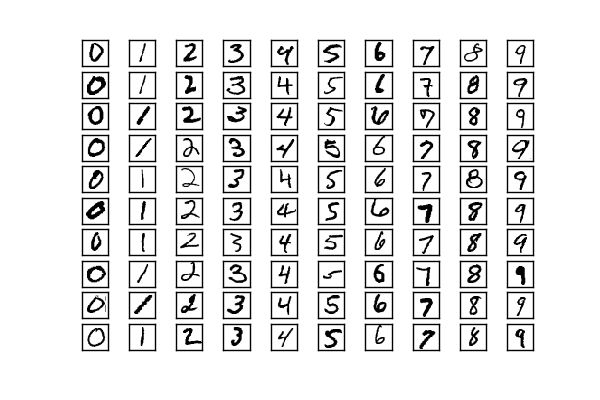
\includegraphics[scale=1.0]{Images/mnist}
	\caption{\label{fig:mnist_example} MNIST sample images having handwritten digits from 0-9, image size is 28x28 and images are grayscale, shown samples are randomly chosen, 10 for each class} 
\end{figure}


\subsection{CIFAR10}
MNIST dataset has50000 training samples and 10000 testing samples.It is database of different objects present in the images. Sample examples are shown in fig.\ref{fig:cifar10_example}

\begin{figure}[H]
	\centering
	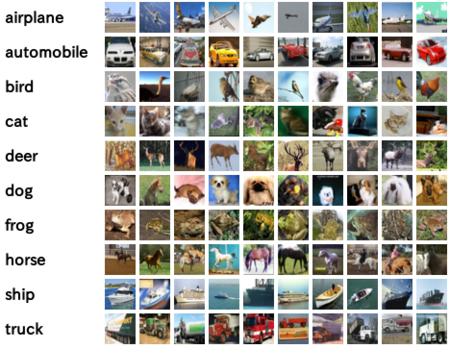
\includegraphics[scale=0.8]{Images/cifar10}
	\caption{\label{fig:cifar10_example} CIFAR-10 sample images having different objects present in the images, image size is 32x32 and images are color,} 
\end{figure}

\subsection{CIFAR100}
CIFAR100 dataset has 50000 training samples and 10000 testing samples.It is database of 100 different object classes. Sample examples are shown in fig.\ref{fig:cif00_example}

\begin{figure}[H]
	\centering
	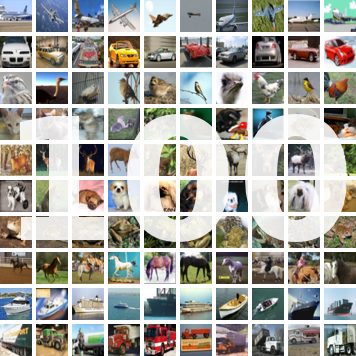
\includegraphics[scale=0.8]{Images/cifar_100}
	\caption{\label{fig:cif00_example} CIFAR-100 sample images consist of database with 100 different object classes, image size is 32x32 and images are color} 
\end{figure}

\subsection{Software}
Keras \cite{chollet2015} is mainly used for almost all the experiments. Theano \cite{2016arXiv160502688short} is used as main backend for Keras.Python is used as main programming language.
% chap2.tex


\chapter{Network Structure}\label{chap:nwstruct}

This chapter discusses different type of networks in practice, their usage and prominent network architectures. We will discuss only few networks which have achieved significant success in recent times. Primarily we will discuss CNN(Convolutional Neural network) as that is the main network used through out this work.

\section{Networks}
The introduction to Neural network has started long ago with Frank Rosenblatt, famous MLP(Multi Layer Perceptron)\cite{Rosenblatt58theperceptron:}.Working of neural nets today are precisely captured by Rosenblatt.
It talks about pathways to connect to output so that for particular input associated pathway gets activated and produces corresponding output.
Following that several networks are suggested directed for specific tasks. For example for image to extract neighborhood relationship, convolution neural networks are suggested. For time series data Recurrent neural networks are suggested. LSTM is recent state of the art for handling time series tasks.

Auto Encoders are suggested as unsupervised nets, which generates low level representation of inputs using only input data. 
Restricted boltzmann machines are another type of network which focuses on convergence by lowering the energy.
In Hopfield network every neuron connects to every other neuron in the network.

Other types of networks are Radial Basis Network(RBN), Gated Recurrent Unit(GRU), Deep belief network(DBN), Generative adversial network(GAN).


\subsection{Perceptron}
The perceptron has been introduced to handle perceptual recognition, generalization and hence the name Perceptron. In this landmark paper Rosenblatt nicely maps the neurons development in human being to perceptron.
For instance connection of nervous system are assumed as random and in neural nets at start mostly random initializations are used.
The original system has said to be capable of plasticity, which allows other neuron output to change over time seeing stimulus applied. And if same or similar stimuli is seen large number of times, will tend to form pathways to same sets of responding cells. This almost sums up the current neural nets, however the network construction, random initializations may differ a lot. 
The perceptron is shown in fig \ref{fig:percep}
\begin{figure}[H]
	\centering
	\subfigure{
		\centering
		\includegraphics[scale=0.75]{Images/perceptron}
	}
	\caption{\label{fig:percep} Perceptron}
	\medskip
	\small
	\begin{flushleft}
		\textit{Regarded as starting point of neural network evolution perceptron is simplest of neural networks. It has  no hidden layers, just inputs with weights and bias term added together with non linear transformation or activation function produces output. Perceptron was limited in their power due to their non-ability to handle non linear target functions, such as XOR.}
	\end{flushleft}
	
\end{figure}


\subsection{CNN}
CNN famously known as Convolutional Neural Network are revolutionary architecture which has provided significant results in many image based learning tasks. CNN takes advantage of neighborhood relationships between data and so image data is natural choice for these networks. see figure \ref{fig:cnn}.


\begin{figure}[H]
	\centering
	\subfigure{
		\centering
		\includegraphics[scale=0.75]{Images/cnn}
	}
	\caption{\label{fig:cnn} CNN}
	\medskip
	\small
	\begin{flushleft}
		\textit{CNN composition is shown in figure \ref{fig:cnn}, This is most common network configuration, however there are many different variations suggested from time to time. CNN works well on data which is having neighborhood relationship such as image has spatial relationship between pixels. Input undergoes convolution to get low level representation with shared weights for the convolution. Generally convolution filter size is 3x3. Immediately after convolution layer there would be pooling layer, which reduces the data representation further. Deepness comes by repeating these layers. At last flatten layer reduces representation to number of classes which activates one of its neuron or provide the output probabilities of image belonging to output class vector.}
	\end{flushleft}
	
\end{figure}


\subsection{RNN}
Recurrent neural nets are having connections to same hidden layer neurons, and thus capable of storing time series data or feedback to be used with next set of input in sequence.

\begin{figure}[H]
\centering
\subfigure{
	\centering
	\includegraphics[scale=0.75]{Images/rnn}
}
\caption{\label{fig:rnn} RNN}
\medskip
\small
\begin{flushleft}
	\textit{Recurrent neural network are useful in case of sequential data, where data at current instance is dependent on previous data instances. Most popular RNN models are language models, where it generates probabilities of existence of any sentence based on underlying language it trained with. Another important application of RNNs are generative models, where in given one word it generates next word. This is possible by RNN having feedback to same neuron or hidden layers. The feedback give this network immense power as unfolding this network it will act as several deep layers which is dependent on RNN ability to store previous information.}
\end{flushleft}

\end{figure}


\subsection{LSTM}
Long Short Term Memory(LSTM) is one type of RNN network which uses LSTM cells.

\subsection{Auto Encoders}
Auto encoders helps in learning representation by using input as output and just keep encoded layers and grow network as deep as possible. Auto encoder has delivered significant results for various tasks including image classification tasks. Auto encoder LSTM is variant of LSTM with Auto encoding capabilities.





%\renewcommand{\baselinestretch}{\spacing}\normalsize
\doublespacing\normalsize

% chap3.tex
\input{initializers_variables.tex}
\chapter{Hyper-Parameters}\label{chap:hyperparams}
\noindent This chapter introduces hyper-parameters. They are not directly related to the machine learning algorithm parameters, but responsible for overall algorithm evolution. For example learning rate dictates the update strength per iteration, choice of initializer can lead to slow or fast convergence, choice of optimizers provide way to update learning parameters($\theta$).

\noindent Other than direct algorithm parameters, we will consider everything else as hyper-parameter. Mainly we will consider following hyper-parameters, which we will discuss and explain the experiments performed with different choices of these parameters and their effect in overall convergence.

\begin{enumerate}
	\item \textbf{Initializer}
	\item \textbf{Optimizer}
	\item \textbf{Batch size}
	\item \textbf{Total parameters}
	\item \textbf{Number of Epochs}
\end{enumerate}

\section{Initializer}

\noindent Initial network condition is described as \textit{"At birth the construction of the most important networks is largely random, subject to a minimum number of constraints"} in \cite{Rosenblatt58theperceptron:} suggests that random initializations can be used to initialize network parameters and constraints could be range of these parameters.

\noindent \textbf{Uniform initialization}, assigns initial weights from $U[-r,\; r]$, where $U$ is uniform distribution, Mostly $r$ is used as small value $\sim0.1$. Another random initialization scheme is \textbf{Normal Initialization}, based on sampling initial weights from normal distribution, $N(0,1)$. These are simple methods which are getting used.

\noindent \textbf{Uniform initialization using fan in} \cite{LeCun:1998:EB:645754.668382} suggests, using fan-in to determine standard deviation $\sigma_i$ and sampling initial weights from $N(0,\sigma_l)$. value of $\sigma_l$ is dependent on fan-in, which is number of inputs to a hidden unit. It is suggested to be chosen as per \ref{eq:le_uni}
\begin{equation}\label{eq:le_uni}
	\sigma_l=\textbf{m}^{-1/2}, where, \; \textbf{m} \; is \; the \; fan \; in
\end{equation}

\noindent \textbf{Normalized initialization} \cite{Glorot10understandingthe} suggest to use uniform weight initialization as per \ref{eq:gl_normal}
\begin{equation}\label{eq:gl_normal}
U[-\frac{{\sqrt{6}}}{{\sqrt{n_l+n_{l+1}}}}, \frac{{\sqrt{6}}}{{\sqrt{n_l+n_{l+1}}}}]
\end{equation}
where $n_l$ and $n_{l+1}$ are total number of units in $l^{th}$ and ${(l+1)}^{th}$ hidden layer respectively. This work on paradigm of maintaining activation variances in feed forward direction and back propagated gradient variances in both the directions.

\noindent For very deep models and to support activation ReLU/PReLU \cite{DBLP:journals/corr/HeZR015} suggests to use slight modification in considering the variance from \cite{Glorot10understandingthe} and the \textbf{initialization scheme becomes zero-mean Gaussian with standard deviation as $\sqrt{2/n_l}$}, where $n_l$ is number of hidden units in $l^{th}$ layer.

\noindent \textbf{Orthogonal random initializations} \cite{DBLP:journals/corr/SaxeMG13} suggests simple initialization scheme where in initial weights are chosen from the random orthogonal matrix satisfying $W^TW=I$. This yield depth independent learning times, which means as depth increases learning time remains same as oppose to suggested initializations in \cite{LeCun:1998:EB:645754.668382} \cite{Glorot10understandingthe} 

\subsection{Experiments}

In this section we analyze the effect of different initializers based on our experiment results.

\subsubsection{CIFAR100}
\textbf{Two Layer, opti=adagrad, batch size=1xc}

\pgfplotstableclear{\dnwonoptinit}
\pgfplotstableclear{\dnwtwoptinit}
\pgfplotstableclear{\dnwfooptinit}
\pgfplotstableclear{\dnwsxoptinit}
\pgfplotstableclear{\dnwegoptinit}
\pgfplotstableclear{\dnwhnoptinit}

\pgfplotstableread[col sep = comma]{ResultsNormal/cifar100_TwoLayer_100B_0E_nadam_gl_n.csv}\dnwonoptinit
\pgfplotstableread[col sep = comma]{ResultsNormal/cifar100_TwoLayer_100B_0E_nadam_gl_u.csv}\dnwtwoptinit
\pgfplotstableread[col sep = comma]{ResultsNormal/cifar100_TwoLayer_100B_0E_nadam_he_u.csv}\dnwfooptinit
\pgfplotstableread[col sep = comma]{ResultsNormal/cifar100_TwoLayer_100B_0E_nadam_norm.csv}\dnwsxoptinit
\pgfplotstableread[col sep = comma]{ResultsNormal/cifar100_TwoLayer_100B_0E_nadam_unif.csv}\dnwegoptinit
\pgfplotstableread[col sep = comma]{ResultsNormal/cifar100_TwoLayer_100B_0E_nadam_zero.csv}\dnwhnoptinit
\providecommand{\initerr}{Error for initial epochs:INIT}
\providecommand{\initacc}{Accuracy for initial epcohs}
\providecommand{\lateerr}{Error for later epochs}
\providecommand{\lateacc}{Accuracy for later epochs}
\providecommand{\boxerr}{Error variation}
\providecommand{\boxacc}{Accuracy variation}

\providecommand{\initfigtitle}{Different batch results for starting 15 epochs }
\providecommand{\initcaption}{to write}

\providecommand{\latefigtitle}{Different batch results for later epochs}
\providecommand{\latecaption}{to write}

\providecommand{\boxerraccfigtitle}{accuracy and error plot for full training epochs}
\providecommand{\boxerracccaption}{to write}

\providecommand{\trtscaption}{to write}
\providecommand	{\ymaxlim}{0.65}

\begin{figure}[H]
	\hspace{-1cm}
	\begin{tabular}{C{.5\textwidth}C{.5\textwidth}}%
		\subfigure [\initerr] {
			\begin{tikzpicture} %
			\begin{axis}[smooth,
			%xlabel={$epochs$}, %
			ylabel={$error$}, %
			height=4cm,%
			width=4cm,%
			legend style={font=\tiny,at={(1,1)},anchor=north east,fill=none, draw=none},%
			xmax=15,%
			yticklabel style={/pgf/number format/.cd,fixed,precision=5},%
			label style = {scale=0.8},%
			tick label style = {scale=0.8},%
			] %
			\addplot+[mark=pentagon*] table[x expr=\coordindex , y={val_loss}, col sep=comma] {\dnwonoptinit};
			\addlegendentry{1xc};%	
			\addplot+[mark=ball] table[x expr=\coordindex , y={val_loss}, col sep=comma] {\dnwtwoptinit};
			\addlegendentry{2xc};%	
			\addplot+[mark=10-pointed star] table[x expr=\coordindex , y={val_loss}, col sep=comma] {\dnwfooptinit};
			\addlegendentry{4xc};%							
			\addplot+[mark=triangle*] table[x expr=\coordindex , y={val_loss}, col sep=comma] {\dnwsxoptinit};
			\addlegendentry{6xc};%							
			\addplot+[mark=halfcircle*] table[x expr=\coordindex , y={val_loss}, col sep=comma] {\dnwegoptinit};
			\addlegendentry{8xc};%							
			\addplot+[mark=otimes*] table[x expr=\coordindex , y={val_loss}, col sep=comma] {\dnwhnoptinit};
			\addlegendentry{10xc};%
			\end{axis} %
			\end{tikzpicture}
		}&
			\subfigure [\initacc] {
			\begin{tikzpicture} %
			\begin{axis}[smooth,
			%xlabel={$epochs$}, %
			ylabel={$accuracy$}, %
			height=4cm,%
			width=4cm,%
			legend style={font=\tiny,at={(1,0)},anchor=south east,fill=none, draw=none},%
			xmax=15,%
			yticklabel style={/pgf/number format/.cd,fixed,precision=5},%
			label style = {scale=0.8},%
			tick label style = {scale=0.8},%
			] %
			\addplot+[mark=pentagon*] table[x expr=\coordindex , y={val_acc}, col sep=comma] {\dnwonoptinit};
			\addlegendentry{1xc};%	
			\addplot+[mark=ball] table[x expr=\coordindex , y={val_acc}, col sep=comma] {\dnwtwoptinit};
			\addlegendentry{2xc};%	
			\addplot+[mark=10-pointed star] table[x expr=\coordindex , y={val_acc}, col sep=comma] {\dnwfooptinit};
			\addlegendentry{4xc};%							
			\addplot+[mark=triangle*] table[x expr=\coordindex , y={val_acc}, col sep=comma] {\dnwsxoptinit};
			\addlegendentry{6xc};%							
			\addplot+[mark=halfcircle*] table[x expr=\coordindex , y={val_acc}, col sep=comma] {\dnwegoptinit};
			\addlegendentry{8xc};%							
			\addplot+[mark=otimes*] table[x expr=\coordindex , y={val_acc}, col sep=comma] {\dnwhnoptinit};
			\addlegendentry{10xc};%
			\end{axis} %
			\end{tikzpicture}
		}\\%
	\end{tabular}%
	\caption {\textit{\initfigtitle}}%
	\medskip
	\small
	\textit{\initcaption}
\end{figure}

\begin{figure}[H]
	\hspace{-1cm}
	\begin{tabular}{C{.5\textwidth}C{.5\textwidth}}%
		\subfigure [\boxerr] {
			\begin{tikzpicture} %
			\begin{axis}[%
			xlabel={\textit{batch size [in multiple of classes]}}, %
			ylabel={\textit{error}}, %
			boxplot/draw direction=y,%
			xtick={1,2,3,4,5,6},%
			xticklabels={1,2, 4, 6, 8, 10},%
			height=4cm,%
			width=6cm,%
			] %
			\addplot+ [boxplot,fill=cyan!10!white] table [x expr=1,y ={val_loss}] {\dnwonoptinit};							
			\addplot+ [boxplot,fill=green!20!white] table [x expr=2,y ={val_loss}] {\dnwtwoptinit};
			\addplot+ [boxplot,fill=orange!20!white] table [x expr=4,y ={val_loss}] {\dnwfooptinit};		
			\addplot+ [boxplot,fill=violet!10!white] table [x expr=6,y ={val_loss}] {\dnwsxoptinit};					
			\addplot+ [boxplot,fill=pink!10!white] table [x expr=8,y ={val_loss}]  {\dnwegoptinit};						
			\addplot+ [boxplot,fill=green!10!white] table [x expr=10,y ={val_loss}] {\dnwhnoptinit};
			\end{axis} %
			\end{tikzpicture}
		}&
		\subfigure [\boxacc] {
			\begin{tikzpicture} %
			\begin{axis}[%
			boxplot/draw direction=y,%
			xtick={1,2,3,4,5,6},%
			xticklabels={1,2, 4, 6, 8, 10},%
			xlabel={\textit{batch size [in multiple of classes]}}, %
			ylabel={\textit{accuracy}}, %
			height=4cm,%
			width=6cm,%
			] %
			\addplot+ [boxplot,fill=cyan!10!white] table [x expr=1,y ={val_acc}] {\dnwonoptinit};							
			\addplot+ [boxplot,fill=green!20!white] table [x expr=2,y ={val_acc}] {\dnwtwoptinit};
			\addplot+ [boxplot,fill=orange!20!white] table [x expr=4,y ={val_acc}] {\dnwfooptinit};		
			\addplot+ [boxplot,fill=violet!10!white] table [x expr=6,y ={val_acc}] {\dnwsxoptinit};					
			\addplot+ [boxplot,fill=pink!10!white] table [x expr=8,y ={val_acc}]  {\dnwegoptinit};						
			\addplot+ [boxplot,fill=green!10!white] table [x expr=10,y ={val_acc}] {\dnwhnoptinit};
			\end{axis}%
			\end{tikzpicture}
		}
	\end{tabular}
	\caption {\textit{\boxerraccfigtitle}}
	\medskip
	\small
	\textit{\boxerracccaption}
\end{figure}

\begin{figure}[H]
\hspace{-1cm}
\begin{tabular}{C{\textwidth}}%
	\subfigure [\lateerr] {
		\begin{tikzpicture} %
		\begin{axis}[smooth,
		xlabel={$epochs$}, %
		ylabel={$error$}, %
		height=3cm,%
		width=12cm,%
		legend style={font=\tiny,legend columns=-1, at={(1,1)},anchor=north east,fill=none, draw=none},%
		xmin=15,%
		yticklabel style={/pgf/number format/.cd,fixed,precision=5},%
		] %
		\addplot+[mark=pentagon*] table[x expr=\coordindex , y={val_loss}, col sep=comma] {\dnwonoptinit};
		\addlegendentry{1xc};%	
		\addplot+[mark=ball] table[x expr=\coordindex , y={val_loss}, col sep=comma] {\dnwtwoptinit};
		\addlegendentry{2xc};%	
		\addplot+[mark=10-pointed star] table[x expr=\coordindex , y={val_loss}, col sep=comma] {\dnwfooptinit};
		\addlegendentry{4xc};%							
		\addplot+[mark=triangle*] table[x expr=\coordindex , y={val_loss}, col sep=comma] {\dnwsxoptinit};
		\addlegendentry{6xc};%							
		\addplot+[mark=halfcircle*] table[x expr=\coordindex , y={val_loss}, col sep=comma] {\dnwegoptinit};
		\addlegendentry{8xc};%							
		\addplot+[mark=otimes*] table[x expr=\coordindex , y={val_loss}, col sep=comma] {\dnwhnoptinit};
		\addlegendentry{10xc};%
		\end{axis} %
		\end{tikzpicture}
	}\\
	\subfigure [\lateacc] {
		\begin{tikzpicture} %
		\begin{axis}[smooth,
		xlabel={$epochs$}, %
		ylabel={$accuracy$}, %
		height=3cm,%
		width=12cm,%
		legend style={font=\tiny,legend columns=-1, at={(1,0)},anchor=south east,fill=none, draw=none},%
		%ymin=\ymaxlim,%
		xmin=12,%
		yticklabel style={/pgf/number format/.cd,fixed,precision=5},%
		] %
		\addplot+[mark=pentagon*] table[x expr=\coordindex , y={val_acc}, col sep=comma] {\dnwonoptinit};
		\addlegendentry{1xc};%	
		\addplot+[mark=ball] table[x expr=\coordindex , y={val_acc}, col sep=comma] {\dnwtwoptinit};
		\addlegendentry{2xc};%	
		\addplot+[mark=10-pointed star] table[x expr=\coordindex , y={val_acc}, col sep=comma] {\dnwfooptinit};
		\addlegendentry{4xc};%							
		\addplot+[mark=triangle*] table[x expr=\coordindex , y={val_acc}, col sep=comma] {\dnwsxoptinit};
		\addlegendentry{6xc};%							
		\addplot+[mark=halfcircle*] table[x expr=\coordindex , y={val_acc}, col sep=comma] {\dnwegoptinit};
		\addlegendentry{8xc};%							
		\addplot+[mark=otimes*] table[x expr=\coordindex , y={val_acc}, col sep=comma] {\dnwhnoptinit};
		\addlegendentry{10xc};%
		\end{axis} %
		\end{tikzpicture}
	}\\
\end{tabular}
\caption {\textit{\latefigtitle}}
\medskip
\small
\textit{\latecaption}
\end{figure}

%

%%%%%%%%%%%%%%%%%%%%%%%%%%%%%%%%%%%%%%%%%%%%%%%%%%%%%%%START%%%%%%%%%%%%%%%%%%%%%%%%%%%%%%%%%%%%%%%%%%%%%%%%%%%
%%%%%%%%%%%%%%%%%%%%%%%%%%%%%%TRAINING VS TESTING ACCURACY AND LOSS FOR ALL BATCH SIZES%%%%%%%%%%%%%%%%%%%%%%%%%
\begin{figure}[H]
	\hspace{-1cm}
	\begin{tabular}{C{.50\textwidth}C{.50\textwidth}}%
		\subfigure [2x-Error] {
			\begin{tikzpicture} %
			\begin{axis}[smooth,
			label style = {scale=0.5},%
			tick label style = {scale=0.5},%
			xlabel={$training$}, %
			ylabel={$testing$}, %
			height=3cm,%
			width=6cm,%
			line width=1,%
			axis y line*=left,%
			legend style={legend columns=-1, at={(1,0)},anchor=south east,fill=red!10!white, draw=none},%
			] %
			\addplot+[blue!80!white,densely dotted,mark=1,fill=red!10!white] table[x={acc} , y={val_acc}] {\dnwtwoptinit};%
			\addlegendentry{accuracy};%						
			\end{axis} %
			\begin{axis}[smooth,
			label style = {scale=0.5},%
			tick label style = {scale=0.5},%
			%xlabel={$training-error$}, %
			%ylabel={$testing-error$}, %
			xticklabel shift={0.5cm},%
			axis line shift=3pt,%
			height=3cm,%
			width=6cm,%
			line width=1,%
			axis y line*=right,%
			legend style={legend columns=-1, at={(0,1)},anchor=north west,fill=blue!10!white, draw=none},%
			] %
			\addplot+[red!80!white,densely dotted,mark=1,fill=blue!10!white] table[x={loss} , y={val_loss}]{\dnwtwoptinit};%
			\addlegendentry{loss};%							
			\end{axis} %
			\end{tikzpicture}			
		}&
		\subfigure [2x-Accuracy] {
			\begin{tikzpicture} %
			\begin{axis}[smooth,
			label style = {scale=0.8},%
			xlabel={$training-error$}, %
			ylabel={$testing-error$}, %
			height=3cm,%
			width=6cm,%
			line width=1,%
			axis y line*=right,%
			legend style={legend columns=-1, at={(0,1)},anchor=north west,fill=blue!10!white, draw=none},%
			] %
			\addplot+[red!80!white,densely dotted,mark=1,fill=blue!10!white] table[x={loss} , y={val_loss}]{\dnwtwoptinit};%
			\addlegendentry{loss};%							
			\end{axis} %
			\end{tikzpicture}
		}\\%
	\subfigure [4x-Error] {
		\begin{tikzpicture} %
		\begin{axis}[smooth,
		xlabel={$training$}, %
		ylabel={$testing$}, %
		height=3cm,%
		width=6cm,%
	    line width=1,%
		] %
		\addplot+[blue!70!white,densely dotted,mark=square,fill=red!20!white] table[x={acc} , y={val_acc}] {\dnwfooptinit};				
		\end{axis} %
		\end{tikzpicture}%			
	}&
	\subfigure [4x-Accuracy] {
		\begin{tikzpicture} %
		\begin{axis}[smooth,
		xlabel={$training$}, %
		ylabel={$testing$}, %
		height=3cm,%
		width=6cm,%
		line width=1,%
		] %
		\addplot+[red!70!white,densely dotted,mark=square,fill=blue!20!white] table[x={loss} , y={val_loss}] {\dnwfooptinit};					
		\end{axis} %
		\end{tikzpicture}
	}\\%
	\subfigure [6x-Error] {
		\begin{tikzpicture} %
		\begin{axis}[smooth,
		xlabel={$training$}, %
		ylabel={$testing$}, %
		height=3cm,%
		width=6cm,%
		line width=1,%
		%ymin=0.992,%
		] %
		\addplot+[mark=square,fill=red!20!white] table[x={acc} , y={val_acc}] {\dnwsxoptinit};				
		\end{axis} %
		\end{tikzpicture}%			
	}&
	\subfigure [6x-Accuracy] {
		\begin{tikzpicture} %
		\begin{axis}[smooth,
		xlabel={$training$}, %
		ylabel={$testing$}, %
		height=3cm,%
		width=6cm,%
		line width=1,%
		] %
		\addplot+[mark=square,fill=red!20!white] table[x={loss} , y={val_loss}] {\dnwsxoptinit};					
		\end{axis} %
		\end{tikzpicture}
	}
	\end{tabular}
	\caption {\textit{\trtscaption}}
\end{figure}

%%%%%%%%%%%%%%%%%%%%%%%%%%%%%%TRAINING VS TESTING ACCURACY AND LOSS FOR ALL BATCH SIZES%%%%%%%%%%%%%%%%%%%%%%%%%
%%%%%%%%%%%%%%%%%%%%%%%%%%%%%%%%%%%%%%%%%%%%%%%%%%%%%%%END%%%%%%%%%%%%%%%%%%%%%%%%%%%%%%%%%%%%%%%%%%%%%%%%%%%


\pgfplotstableclear{\dnwonoptinit}
\pgfplotstableclear{\dnwtwoptinit}
\pgfplotstableclear{\dnwfooptinit}
\pgfplotstableclear{\dnwsxoptinit}
\pgfplotstableclear{\dnwegoptinit}
\pgfplotstableclear{\dnwhnoptinit}

\relax


\textbf{Two Layer, opti=SGD with nesterov momentum, batch size=1xc}

\pgfplotstableread[col sep = comma]{ResultsNormal/cifar100_TwoLayer_100B_0E_SGD_gl_n.csv}\dnwonoptinit
\pgfplotstableread[col sep = comma]{ResultsNormal/cifar100_TwoLayer_100B_0E_SGD_gl_u.csv}\dnwtwoptinit
\pgfplotstableread[col sep = comma]{ResultsNormal/cifar100_TwoLayer_100B_0E_SGD_he_u.csv}\dnwfooptinit
\pgfplotstableread[col sep = comma]{ResultsNormal/cifar100_TwoLayer_100B_0E_SGD_norm.csv}\dnwsxoptinit
\pgfplotstableread[col sep = comma]{ResultsNormal/cifar100_TwoLayer_100B_0E_SGD_unif.csv}\dnwegoptinit
\pgfplotstableread[col sep = comma]{ResultsNormal/cifar100_TwoLayer_100B_0E_SGD_zero.csv}\dnwhnoptinit
\renewcommand{\initerr}{Error for initial epochs:INIT}
\renewcommand{\initacc}{Accuracy for initial epcohs}
\renewcommand{\lateerr}{Error for later epochs}
\renewcommand{\lateacc}{Accuracy for later epochs}
\renewcommand{\boxerr}{Error variation}
\renewcommand{\boxacc}{Accuracy variation}

\renewcommand{\initfigtitle}{Different batch results for starting 15 epochs }
\renewcommand{\initcaption}{to write}

\renewcommand{\latefigtitle}{Different batch results for later epochs}
\renewcommand{\latecaption}{to write}

\renewcommand{\boxerraccfigtitle}{accuracy and error plot for full training epochs}
\renewcommand{\boxerracccaption}{to write}

\renewcommand{\trtscaption}{to write}
\renewcommand	{\ymaxlim}{0.65}

\begin{figure}[H]
	\hspace{-1cm}
	\begin{tabular}{C{.5\textwidth}C{.5\textwidth}}%
		\subfigure [\initerr] {
			\begin{tikzpicture} %
			\begin{axis}[smooth,
			%xlabel={$epochs$}, %
			ylabel={$error$}, %
			height=4cm,%
			width=4cm,%
			legend style={font=\tiny,at={(1,1)},anchor=north east,fill=none, draw=none},%
			xmax=15,%
			yticklabel style={/pgf/number format/.cd,fixed,precision=5},%
			label style = {scale=0.8},%
			tick label style = {scale=0.8},%
			] %
			\addplot+[mark=pentagon*] table[x expr=\coordindex , y={val_loss}, col sep=comma] {\dnwonoptinit};
			\addlegendentry{1xc};%	
			\addplot+[mark=ball] table[x expr=\coordindex , y={val_loss}, col sep=comma] {\dnwtwoptinit};
			\addlegendentry{2xc};%	
			\addplot+[mark=10-pointed star] table[x expr=\coordindex , y={val_loss}, col sep=comma] {\dnwfooptinit};
			\addlegendentry{4xc};%							
			\addplot+[mark=triangle*] table[x expr=\coordindex , y={val_loss}, col sep=comma] {\dnwsxoptinit};
			\addlegendentry{6xc};%							
			\addplot+[mark=halfcircle*] table[x expr=\coordindex , y={val_loss}, col sep=comma] {\dnwegoptinit};
			\addlegendentry{8xc};%							
			\addplot+[mark=otimes*] table[x expr=\coordindex , y={val_loss}, col sep=comma] {\dnwhnoptinit};
			\addlegendentry{10xc};%
			\end{axis} %
			\end{tikzpicture}
		}&
			\subfigure [\initacc] {
			\begin{tikzpicture} %
			\begin{axis}[smooth,
			%xlabel={$epochs$}, %
			ylabel={$accuracy$}, %
			height=4cm,%
			width=4cm,%
			legend style={font=\tiny,at={(1,0)},anchor=south east,fill=none, draw=none},%
			xmax=15,%
			yticklabel style={/pgf/number format/.cd,fixed,precision=5},%
			label style = {scale=0.8},%
			tick label style = {scale=0.8},%
			] %
			\addplot+[mark=pentagon*] table[x expr=\coordindex , y={val_acc}, col sep=comma] {\dnwonoptinit};
			\addlegendentry{1xc};%	
			\addplot+[mark=ball] table[x expr=\coordindex , y={val_acc}, col sep=comma] {\dnwtwoptinit};
			\addlegendentry{2xc};%	
			\addplot+[mark=10-pointed star] table[x expr=\coordindex , y={val_acc}, col sep=comma] {\dnwfooptinit};
			\addlegendentry{4xc};%							
			\addplot+[mark=triangle*] table[x expr=\coordindex , y={val_acc}, col sep=comma] {\dnwsxoptinit};
			\addlegendentry{6xc};%							
			\addplot+[mark=halfcircle*] table[x expr=\coordindex , y={val_acc}, col sep=comma] {\dnwegoptinit};
			\addlegendentry{8xc};%							
			\addplot+[mark=otimes*] table[x expr=\coordindex , y={val_acc}, col sep=comma] {\dnwhnoptinit};
			\addlegendentry{10xc};%
			\end{axis} %
			\end{tikzpicture}
		}\\%
	\end{tabular}%
	\caption {\textit{\initfigtitle}}%
	\medskip
	\small
	\textit{\initcaption}
\end{figure}

\begin{figure}[H]
	\hspace{-1cm}
	\begin{tabular}{C{.5\textwidth}C{.5\textwidth}}%
		\subfigure [\boxerr] {
			\begin{tikzpicture} %
			\begin{axis}[%
			xlabel={\textit{batch size [in multiple of classes]}}, %
			ylabel={\textit{error}}, %
			boxplot/draw direction=y,%
			xtick={1,2,3,4,5,6},%
			xticklabels={1,2, 4, 6, 8, 10},%
			height=4cm,%
			width=6cm,%
			] %
			\addplot+ [boxplot,fill=cyan!10!white] table [x expr=1,y ={val_loss}] {\dnwonoptinit};							
			\addplot+ [boxplot,fill=green!20!white] table [x expr=2,y ={val_loss}] {\dnwtwoptinit};
			\addplot+ [boxplot,fill=orange!20!white] table [x expr=4,y ={val_loss}] {\dnwfooptinit};		
			\addplot+ [boxplot,fill=violet!10!white] table [x expr=6,y ={val_loss}] {\dnwsxoptinit};					
			\addplot+ [boxplot,fill=pink!10!white] table [x expr=8,y ={val_loss}]  {\dnwegoptinit};						
			\addplot+ [boxplot,fill=green!10!white] table [x expr=10,y ={val_loss}] {\dnwhnoptinit};
			\end{axis} %
			\end{tikzpicture}
		}&
		\subfigure [\boxacc] {
			\begin{tikzpicture} %
			\begin{axis}[%
			boxplot/draw direction=y,%
			xtick={1,2,3,4,5,6},%
			xticklabels={1,2, 4, 6, 8, 10},%
			xlabel={\textit{batch size [in multiple of classes]}}, %
			ylabel={\textit{accuracy}}, %
			height=4cm,%
			width=6cm,%
			] %
			\addplot+ [boxplot,fill=cyan!10!white] table [x expr=1,y ={val_acc}] {\dnwonoptinit};							
			\addplot+ [boxplot,fill=green!20!white] table [x expr=2,y ={val_acc}] {\dnwtwoptinit};
			\addplot+ [boxplot,fill=orange!20!white] table [x expr=4,y ={val_acc}] {\dnwfooptinit};		
			\addplot+ [boxplot,fill=violet!10!white] table [x expr=6,y ={val_acc}] {\dnwsxoptinit};					
			\addplot+ [boxplot,fill=pink!10!white] table [x expr=8,y ={val_acc}]  {\dnwegoptinit};						
			\addplot+ [boxplot,fill=green!10!white] table [x expr=10,y ={val_acc}] {\dnwhnoptinit};
			\end{axis}%
			\end{tikzpicture}
		}
	\end{tabular}
	\caption {\textit{\boxerraccfigtitle}}
	\medskip
	\small
	\textit{\boxerracccaption}
\end{figure}

\begin{figure}[H]
\hspace{-1cm}
\begin{tabular}{C{\textwidth}}%
	\subfigure [\lateerr] {
		\begin{tikzpicture} %
		\begin{axis}[smooth,
		xlabel={$epochs$}, %
		ylabel={$error$}, %
		height=3cm,%
		width=12cm,%
		legend style={font=\tiny,legend columns=-1, at={(1,1)},anchor=north east,fill=none, draw=none},%
		xmin=15,%
		yticklabel style={/pgf/number format/.cd,fixed,precision=5},%
		] %
		\addplot+[mark=pentagon*] table[x expr=\coordindex , y={val_loss}, col sep=comma] {\dnwonoptinit};
		\addlegendentry{1xc};%	
		\addplot+[mark=ball] table[x expr=\coordindex , y={val_loss}, col sep=comma] {\dnwtwoptinit};
		\addlegendentry{2xc};%	
		\addplot+[mark=10-pointed star] table[x expr=\coordindex , y={val_loss}, col sep=comma] {\dnwfooptinit};
		\addlegendentry{4xc};%							
		\addplot+[mark=triangle*] table[x expr=\coordindex , y={val_loss}, col sep=comma] {\dnwsxoptinit};
		\addlegendentry{6xc};%							
		\addplot+[mark=halfcircle*] table[x expr=\coordindex , y={val_loss}, col sep=comma] {\dnwegoptinit};
		\addlegendentry{8xc};%							
		\addplot+[mark=otimes*] table[x expr=\coordindex , y={val_loss}, col sep=comma] {\dnwhnoptinit};
		\addlegendentry{10xc};%
		\end{axis} %
		\end{tikzpicture}
	}\\
	\subfigure [\lateacc] {
		\begin{tikzpicture} %
		\begin{axis}[smooth,
		xlabel={$epochs$}, %
		ylabel={$accuracy$}, %
		height=3cm,%
		width=12cm,%
		legend style={font=\tiny,legend columns=-1, at={(1,0)},anchor=south east,fill=none, draw=none},%
		%ymin=\ymaxlim,%
		xmin=12,%
		yticklabel style={/pgf/number format/.cd,fixed,precision=5},%
		] %
		\addplot+[mark=pentagon*] table[x expr=\coordindex , y={val_acc}, col sep=comma] {\dnwonoptinit};
		\addlegendentry{1xc};%	
		\addplot+[mark=ball] table[x expr=\coordindex , y={val_acc}, col sep=comma] {\dnwtwoptinit};
		\addlegendentry{2xc};%	
		\addplot+[mark=10-pointed star] table[x expr=\coordindex , y={val_acc}, col sep=comma] {\dnwfooptinit};
		\addlegendentry{4xc};%							
		\addplot+[mark=triangle*] table[x expr=\coordindex , y={val_acc}, col sep=comma] {\dnwsxoptinit};
		\addlegendentry{6xc};%							
		\addplot+[mark=halfcircle*] table[x expr=\coordindex , y={val_acc}, col sep=comma] {\dnwegoptinit};
		\addlegendentry{8xc};%							
		\addplot+[mark=otimes*] table[x expr=\coordindex , y={val_acc}, col sep=comma] {\dnwhnoptinit};
		\addlegendentry{10xc};%
		\end{axis} %
		\end{tikzpicture}
	}\\
\end{tabular}
\caption {\textit{\latefigtitle}}
\medskip
\small
\textit{\latecaption}
\end{figure}

%

%%%%%%%%%%%%%%%%%%%%%%%%%%%%%%%%%%%%%%%%%%%%%%%%%%%%%%%START%%%%%%%%%%%%%%%%%%%%%%%%%%%%%%%%%%%%%%%%%%%%%%%%%%%
%%%%%%%%%%%%%%%%%%%%%%%%%%%%%%TRAINING VS TESTING ACCURACY AND LOSS FOR ALL BATCH SIZES%%%%%%%%%%%%%%%%%%%%%%%%%
\begin{figure}[H]
	\hspace{-1cm}
	\begin{tabular}{C{.50\textwidth}C{.50\textwidth}}%
		\subfigure [2x-Error] {
			\begin{tikzpicture} %
			\begin{axis}[smooth,
			label style = {scale=0.5},%
			tick label style = {scale=0.5},%
			xlabel={$training$}, %
			ylabel={$testing$}, %
			height=3cm,%
			width=6cm,%
			line width=1,%
			axis y line*=left,%
			legend style={legend columns=-1, at={(1,0)},anchor=south east,fill=red!10!white, draw=none},%
			] %
			\addplot+[blue!80!white,densely dotted,mark=1,fill=red!10!white] table[x={acc} , y={val_acc}] {\dnwtwoptinit};%
			\addlegendentry{accuracy};%						
			\end{axis} %
			\begin{axis}[smooth,
			label style = {scale=0.5},%
			tick label style = {scale=0.5},%
			%xlabel={$training-error$}, %
			%ylabel={$testing-error$}, %
			xticklabel shift={0.5cm},%
			axis line shift=3pt,%
			height=3cm,%
			width=6cm,%
			line width=1,%
			axis y line*=right,%
			legend style={legend columns=-1, at={(0,1)},anchor=north west,fill=blue!10!white, draw=none},%
			] %
			\addplot+[red!80!white,densely dotted,mark=1,fill=blue!10!white] table[x={loss} , y={val_loss}]{\dnwtwoptinit};%
			\addlegendentry{loss};%							
			\end{axis} %
			\end{tikzpicture}			
		}&
		\subfigure [2x-Accuracy] {
			\begin{tikzpicture} %
			\begin{axis}[smooth,
			label style = {scale=0.8},%
			xlabel={$training-error$}, %
			ylabel={$testing-error$}, %
			height=3cm,%
			width=6cm,%
			line width=1,%
			axis y line*=right,%
			legend style={legend columns=-1, at={(0,1)},anchor=north west,fill=blue!10!white, draw=none},%
			] %
			\addplot+[red!80!white,densely dotted,mark=1,fill=blue!10!white] table[x={loss} , y={val_loss}]{\dnwtwoptinit};%
			\addlegendentry{loss};%							
			\end{axis} %
			\end{tikzpicture}
		}\\%
	\subfigure [4x-Error] {
		\begin{tikzpicture} %
		\begin{axis}[smooth,
		xlabel={$training$}, %
		ylabel={$testing$}, %
		height=3cm,%
		width=6cm,%
	    line width=1,%
		] %
		\addplot+[blue!70!white,densely dotted,mark=square,fill=red!20!white] table[x={acc} , y={val_acc}] {\dnwfooptinit};				
		\end{axis} %
		\end{tikzpicture}%			
	}&
	\subfigure [4x-Accuracy] {
		\begin{tikzpicture} %
		\begin{axis}[smooth,
		xlabel={$training$}, %
		ylabel={$testing$}, %
		height=3cm,%
		width=6cm,%
		line width=1,%
		] %
		\addplot+[red!70!white,densely dotted,mark=square,fill=blue!20!white] table[x={loss} , y={val_loss}] {\dnwfooptinit};					
		\end{axis} %
		\end{tikzpicture}
	}\\%
	\subfigure [6x-Error] {
		\begin{tikzpicture} %
		\begin{axis}[smooth,
		xlabel={$training$}, %
		ylabel={$testing$}, %
		height=3cm,%
		width=6cm,%
		line width=1,%
		%ymin=0.992,%
		] %
		\addplot+[mark=square,fill=red!20!white] table[x={acc} , y={val_acc}] {\dnwsxoptinit};				
		\end{axis} %
		\end{tikzpicture}%			
	}&
	\subfigure [6x-Accuracy] {
		\begin{tikzpicture} %
		\begin{axis}[smooth,
		xlabel={$training$}, %
		ylabel={$testing$}, %
		height=3cm,%
		width=6cm,%
		line width=1,%
		] %
		\addplot+[mark=square,fill=red!20!white] table[x={loss} , y={val_loss}] {\dnwsxoptinit};					
		\end{axis} %
		\end{tikzpicture}
	}
	\end{tabular}
	\caption {\textit{\trtscaption}}
\end{figure}

%%%%%%%%%%%%%%%%%%%%%%%%%%%%%%TRAINING VS TESTING ACCURACY AND LOSS FOR ALL BATCH SIZES%%%%%%%%%%%%%%%%%%%%%%%%%
%%%%%%%%%%%%%%%%%%%%%%%%%%%%%%%%%%%%%%%%%%%%%%%%%%%%%%%END%%%%%%%%%%%%%%%%%%%%%%%%%%%%%%%%%%%%%%%%%%%%%%%%%%%


\pgfplotstableclear{\dnwonoptinit}
\pgfplotstableclear{\dnwtwoptinit}
\pgfplotstableclear{\dnwfooptinit}
\pgfplotstableclear{\dnwsxoptinit}
\pgfplotstableclear{\dnwegoptinit}
\pgfplotstableclear{\dnwhnoptinit}

\relax


\subsubsection{CIFAR-10}
\textbf{Five Layer, opti=adagrad, batch size=2xc}

\pgfplotstableclear{\dnwonoptinit}
\pgfplotstableclear{\dnwtwoptinit}
\pgfplotstableclear{\dnwfooptinit}
\pgfplotstableclear{\dnwsxoptinit}
\pgfplotstableclear{\dnwegoptinit}
\pgfplotstableclear{\dnwhnoptinit}

\pgfplotstableread[col sep = comma]{ResultsNormal/cifar10_FiveLayer_20B_0E_adagrad_gl_n.csv}\dnwonoptinit
\pgfplotstableread[col sep = comma]{ResultsNormal/cifar10_FiveLayer_20B_0E_adagrad_gl_u.csv}\dnwtwoptinit
\pgfplotstableread[col sep = comma]{ResultsNormal/cifar10_FiveLayer_20B_0E_adagrad_he_u.csv}\dnwfooptinit
\pgfplotstableread[col sep = comma]{ResultsNormal/cifar10_FiveLayer_20B_0E_adagrad_norm.csv}\dnwsxoptinit
\pgfplotstableread[col sep = comma]{ResultsNormal/cifar10_FiveLayer_20B_0E_adagrad_unif.csv}\dnwegoptinit
\pgfplotstableread[col sep = comma]{ResultsNormal/cifar10_FiveLayer_20B_0E_adagrad_zero.csv}\dnwhnoptinit
\renewcommand{\initerr}{Error for initiaNITCIFAR10}
\renewcommand{\initacc}{Accuracy for initial epcohs}
\renewcommand{\lateerr}{Error for later epochs}
\renewcommand{\lateacc}{Accuracy for later epochs}
\renewcommand{\boxerr}{Error variation}
\renewcommand{\boxacc}{Accuracy variation}

\renewcommand{\initfigtitle}{Different batch results for starting 15 epochs }
\renewcommand{\initcaption}{to write}

\renewcommand{\latefigtitle}{Different batch results for later epochs}
\renewcommand{\latecaption}{to write}

\renewcommand{\boxerraccfigtitle}{accuracy and error plot for full training epochs}
\renewcommand{\boxerracccaption}{to write}

\renewcommand{\trtscaption}{to write}
\renewcommand	{\ymaxlim}{0.65}

\begin{figure}[H]
	\hspace{-1cm}
	\begin{tabular}{C{.5\textwidth}C{.5\textwidth}}%
		\subfigure [\initerr] {
			\begin{tikzpicture} %
			\begin{axis}[smooth,
			%xlabel={$epochs$}, %
			ylabel={$error$}, %
			height=4cm,%
			width=4cm,%
			legend style={font=\tiny,at={(1,1)},anchor=north east,fill=none, draw=none},%
			xmax=15,%
			yticklabel style={/pgf/number format/.cd,fixed,precision=5},%
			label style = {scale=0.8},%
			tick label style = {scale=0.8},%
			] %
			\addplot+[mark=pentagon*] table[x expr=\coordindex , y={val_loss}, col sep=comma] {\dnwonoptinit};
			\addlegendentry{1xc};%	
			\addplot+[mark=ball] table[x expr=\coordindex , y={val_loss}, col sep=comma] {\dnwtwoptinit};
			\addlegendentry{2xc};%	
			\addplot+[mark=10-pointed star] table[x expr=\coordindex , y={val_loss}, col sep=comma] {\dnwfooptinit};
			\addlegendentry{4xc};%							
			\addplot+[mark=triangle*] table[x expr=\coordindex , y={val_loss}, col sep=comma] {\dnwsxoptinit};
			\addlegendentry{6xc};%							
			\addplot+[mark=halfcircle*] table[x expr=\coordindex , y={val_loss}, col sep=comma] {\dnwegoptinit};
			\addlegendentry{8xc};%							
			\addplot+[mark=otimes*] table[x expr=\coordindex , y={val_loss}, col sep=comma] {\dnwhnoptinit};
			\addlegendentry{10xc};%
			\end{axis} %
			\end{tikzpicture}
		}&
			\subfigure [\initacc] {
			\begin{tikzpicture} %
			\begin{axis}[smooth,
			%xlabel={$epochs$}, %
			ylabel={$accuracy$}, %
			height=4cm,%
			width=4cm,%
			legend style={font=\tiny,at={(1,0)},anchor=south east,fill=none, draw=none},%
			xmax=15,%
			yticklabel style={/pgf/number format/.cd,fixed,precision=5},%
			label style = {scale=0.8},%
			tick label style = {scale=0.8},%
			] %
			\addplot+[mark=pentagon*] table[x expr=\coordindex , y={val_acc}, col sep=comma] {\dnwonoptinit};
			\addlegendentry{1xc};%	
			\addplot+[mark=ball] table[x expr=\coordindex , y={val_acc}, col sep=comma] {\dnwtwoptinit};
			\addlegendentry{2xc};%	
			\addplot+[mark=10-pointed star] table[x expr=\coordindex , y={val_acc}, col sep=comma] {\dnwfooptinit};
			\addlegendentry{4xc};%							
			\addplot+[mark=triangle*] table[x expr=\coordindex , y={val_acc}, col sep=comma] {\dnwsxoptinit};
			\addlegendentry{6xc};%							
			\addplot+[mark=halfcircle*] table[x expr=\coordindex , y={val_acc}, col sep=comma] {\dnwegoptinit};
			\addlegendentry{8xc};%							
			\addplot+[mark=otimes*] table[x expr=\coordindex , y={val_acc}, col sep=comma] {\dnwhnoptinit};
			\addlegendentry{10xc};%
			\end{axis} %
			\end{tikzpicture}
		}\\%
	\end{tabular}%
	\caption {\textit{\initfigtitle}}%
	\medskip
	\small
	\textit{\initcaption}
\end{figure}

\begin{figure}[H]
	\hspace{-1cm}
	\begin{tabular}{C{.5\textwidth}C{.5\textwidth}}%
		\subfigure [\boxerr] {
			\begin{tikzpicture} %
			\begin{axis}[%
			xlabel={\textit{batch size [in multiple of classes]}}, %
			ylabel={\textit{error}}, %
			boxplot/draw direction=y,%
			xtick={1,2,3,4,5,6},%
			xticklabels={1,2, 4, 6, 8, 10},%
			height=4cm,%
			width=6cm,%
			] %
			\addplot+ [boxplot,fill=cyan!10!white] table [x expr=1,y ={val_loss}] {\dnwonoptinit};							
			\addplot+ [boxplot,fill=green!20!white] table [x expr=2,y ={val_loss}] {\dnwtwoptinit};
			\addplot+ [boxplot,fill=orange!20!white] table [x expr=4,y ={val_loss}] {\dnwfooptinit};		
			\addplot+ [boxplot,fill=violet!10!white] table [x expr=6,y ={val_loss}] {\dnwsxoptinit};					
			\addplot+ [boxplot,fill=pink!10!white] table [x expr=8,y ={val_loss}]  {\dnwegoptinit};						
			\addplot+ [boxplot,fill=green!10!white] table [x expr=10,y ={val_loss}] {\dnwhnoptinit};
			\end{axis} %
			\end{tikzpicture}
		}&
		\subfigure [\boxacc] {
			\begin{tikzpicture} %
			\begin{axis}[%
			boxplot/draw direction=y,%
			xtick={1,2,3,4,5,6},%
			xticklabels={1,2, 4, 6, 8, 10},%
			xlabel={\textit{batch size [in multiple of classes]}}, %
			ylabel={\textit{accuracy}}, %
			height=4cm,%
			width=6cm,%
			] %
			\addplot+ [boxplot,fill=cyan!10!white] table [x expr=1,y ={val_acc}] {\dnwonoptinit};							
			\addplot+ [boxplot,fill=green!20!white] table [x expr=2,y ={val_acc}] {\dnwtwoptinit};
			\addplot+ [boxplot,fill=orange!20!white] table [x expr=4,y ={val_acc}] {\dnwfooptinit};		
			\addplot+ [boxplot,fill=violet!10!white] table [x expr=6,y ={val_acc}] {\dnwsxoptinit};					
			\addplot+ [boxplot,fill=pink!10!white] table [x expr=8,y ={val_acc}]  {\dnwegoptinit};						
			\addplot+ [boxplot,fill=green!10!white] table [x expr=10,y ={val_acc}] {\dnwhnoptinit};
			\end{axis}%
			\end{tikzpicture}
		}
	\end{tabular}
	\caption {\textit{\boxerraccfigtitle}}
	\medskip
	\small
	\textit{\boxerracccaption}
\end{figure}

\begin{figure}[H]
\hspace{-1cm}
\begin{tabular}{C{\textwidth}}%
	\subfigure [\lateerr] {
		\begin{tikzpicture} %
		\begin{axis}[smooth,
		xlabel={$epochs$}, %
		ylabel={$error$}, %
		height=3cm,%
		width=12cm,%
		legend style={font=\tiny,legend columns=-1, at={(1,1)},anchor=north east,fill=none, draw=none},%
		xmin=15,%
		yticklabel style={/pgf/number format/.cd,fixed,precision=5},%
		] %
		\addplot+[mark=pentagon*] table[x expr=\coordindex , y={val_loss}, col sep=comma] {\dnwonoptinit};
		\addlegendentry{1xc};%	
		\addplot+[mark=ball] table[x expr=\coordindex , y={val_loss}, col sep=comma] {\dnwtwoptinit};
		\addlegendentry{2xc};%	
		\addplot+[mark=10-pointed star] table[x expr=\coordindex , y={val_loss}, col sep=comma] {\dnwfooptinit};
		\addlegendentry{4xc};%							
		\addplot+[mark=triangle*] table[x expr=\coordindex , y={val_loss}, col sep=comma] {\dnwsxoptinit};
		\addlegendentry{6xc};%							
		\addplot+[mark=halfcircle*] table[x expr=\coordindex , y={val_loss}, col sep=comma] {\dnwegoptinit};
		\addlegendentry{8xc};%							
		\addplot+[mark=otimes*] table[x expr=\coordindex , y={val_loss}, col sep=comma] {\dnwhnoptinit};
		\addlegendentry{10xc};%
		\end{axis} %
		\end{tikzpicture}
	}\\
	\subfigure [\lateacc] {
		\begin{tikzpicture} %
		\begin{axis}[smooth,
		xlabel={$epochs$}, %
		ylabel={$accuracy$}, %
		height=3cm,%
		width=12cm,%
		legend style={font=\tiny,legend columns=-1, at={(1,0)},anchor=south east,fill=none, draw=none},%
		%ymin=\ymaxlim,%
		xmin=12,%
		yticklabel style={/pgf/number format/.cd,fixed,precision=5},%
		] %
		\addplot+[mark=pentagon*] table[x expr=\coordindex , y={val_acc}, col sep=comma] {\dnwonoptinit};
		\addlegendentry{1xc};%	
		\addplot+[mark=ball] table[x expr=\coordindex , y={val_acc}, col sep=comma] {\dnwtwoptinit};
		\addlegendentry{2xc};%	
		\addplot+[mark=10-pointed star] table[x expr=\coordindex , y={val_acc}, col sep=comma] {\dnwfooptinit};
		\addlegendentry{4xc};%							
		\addplot+[mark=triangle*] table[x expr=\coordindex , y={val_acc}, col sep=comma] {\dnwsxoptinit};
		\addlegendentry{6xc};%							
		\addplot+[mark=halfcircle*] table[x expr=\coordindex , y={val_acc}, col sep=comma] {\dnwegoptinit};
		\addlegendentry{8xc};%							
		\addplot+[mark=otimes*] table[x expr=\coordindex , y={val_acc}, col sep=comma] {\dnwhnoptinit};
		\addlegendentry{10xc};%
		\end{axis} %
		\end{tikzpicture}
	}\\
\end{tabular}
\caption {\textit{\latefigtitle}}
\medskip
\small
\textit{\latecaption}
\end{figure}

%

%%%%%%%%%%%%%%%%%%%%%%%%%%%%%%%%%%%%%%%%%%%%%%%%%%%%%%%START%%%%%%%%%%%%%%%%%%%%%%%%%%%%%%%%%%%%%%%%%%%%%%%%%%%
%%%%%%%%%%%%%%%%%%%%%%%%%%%%%%TRAINING VS TESTING ACCURACY AND LOSS FOR ALL BATCH SIZES%%%%%%%%%%%%%%%%%%%%%%%%%
\begin{figure}[H]
	\hspace{-1cm}
	\begin{tabular}{C{.50\textwidth}C{.50\textwidth}}%
		\subfigure [2x-Error] {
			\begin{tikzpicture} %
			\begin{axis}[smooth,
			label style = {scale=0.5},%
			tick label style = {scale=0.5},%
			xlabel={$training$}, %
			ylabel={$testing$}, %
			height=3cm,%
			width=6cm,%
			line width=1,%
			axis y line*=left,%
			legend style={legend columns=-1, at={(1,0)},anchor=south east,fill=red!10!white, draw=none},%
			] %
			\addplot+[blue!80!white,densely dotted,mark=1,fill=red!10!white] table[x={acc} , y={val_acc}] {\dnwtwoptinit};%
			\addlegendentry{accuracy};%						
			\end{axis} %
			\begin{axis}[smooth,
			label style = {scale=0.5},%
			tick label style = {scale=0.5},%
			%xlabel={$training-error$}, %
			%ylabel={$testing-error$}, %
			xticklabel shift={0.5cm},%
			axis line shift=3pt,%
			height=3cm,%
			width=6cm,%
			line width=1,%
			axis y line*=right,%
			legend style={legend columns=-1, at={(0,1)},anchor=north west,fill=blue!10!white, draw=none},%
			] %
			\addplot+[red!80!white,densely dotted,mark=1,fill=blue!10!white] table[x={loss} , y={val_loss}]{\dnwtwoptinit};%
			\addlegendentry{loss};%							
			\end{axis} %
			\end{tikzpicture}			
		}&
		\subfigure [2x-Accuracy] {
			\begin{tikzpicture} %
			\begin{axis}[smooth,
			label style = {scale=0.8},%
			xlabel={$training-error$}, %
			ylabel={$testing-error$}, %
			height=3cm,%
			width=6cm,%
			line width=1,%
			axis y line*=right,%
			legend style={legend columns=-1, at={(0,1)},anchor=north west,fill=blue!10!white, draw=none},%
			] %
			\addplot+[red!80!white,densely dotted,mark=1,fill=blue!10!white] table[x={loss} , y={val_loss}]{\dnwtwoptinit};%
			\addlegendentry{loss};%							
			\end{axis} %
			\end{tikzpicture}
		}\\%
	\subfigure [4x-Error] {
		\begin{tikzpicture} %
		\begin{axis}[smooth,
		xlabel={$training$}, %
		ylabel={$testing$}, %
		height=3cm,%
		width=6cm,%
	    line width=1,%
		] %
		\addplot+[blue!70!white,densely dotted,mark=square,fill=red!20!white] table[x={acc} , y={val_acc}] {\dnwfooptinit};				
		\end{axis} %
		\end{tikzpicture}%			
	}&
	\subfigure [4x-Accuracy] {
		\begin{tikzpicture} %
		\begin{axis}[smooth,
		xlabel={$training$}, %
		ylabel={$testing$}, %
		height=3cm,%
		width=6cm,%
		line width=1,%
		] %
		\addplot+[red!70!white,densely dotted,mark=square,fill=blue!20!white] table[x={loss} , y={val_loss}] {\dnwfooptinit};					
		\end{axis} %
		\end{tikzpicture}
	}\\%
	\subfigure [6x-Error] {
		\begin{tikzpicture} %
		\begin{axis}[smooth,
		xlabel={$training$}, %
		ylabel={$testing$}, %
		height=3cm,%
		width=6cm,%
		line width=1,%
		%ymin=0.992,%
		] %
		\addplot+[mark=square,fill=red!20!white] table[x={acc} , y={val_acc}] {\dnwsxoptinit};				
		\end{axis} %
		\end{tikzpicture}%			
	}&
	\subfigure [6x-Accuracy] {
		\begin{tikzpicture} %
		\begin{axis}[smooth,
		xlabel={$training$}, %
		ylabel={$testing$}, %
		height=3cm,%
		width=6cm,%
		line width=1,%
		] %
		\addplot+[mark=square,fill=red!20!white] table[x={loss} , y={val_loss}] {\dnwsxoptinit};					
		\end{axis} %
		\end{tikzpicture}
	}
	\end{tabular}
	\caption {\textit{\trtscaption}}
\end{figure}

%%%%%%%%%%%%%%%%%%%%%%%%%%%%%%TRAINING VS TESTING ACCURACY AND LOSS FOR ALL BATCH SIZES%%%%%%%%%%%%%%%%%%%%%%%%%
%%%%%%%%%%%%%%%%%%%%%%%%%%%%%%%%%%%%%%%%%%%%%%%%%%%%%%%END%%%%%%%%%%%%%%%%%%%%%%%%%%%%%%%%%%%%%%%%%%%%%%%%%%%


\pgfplotstableclear{\dnwonoptinit}
\pgfplotstableclear{\dnwtwoptinit}
\pgfplotstableclear{\dnwfooptinit}
\pgfplotstableclear{\dnwsxoptinit}
\pgfplotstableclear{\dnwegoptinit}
\pgfplotstableclear{\dnwhnoptinit}

\relax

\subsubsection{MNIST}
\textbf{Two Layer, opti=nadam, batch size=1xc}






\section{Optimizers}

\noindent Optimizers are main learning algorithm or routine which is responsible for changes in the network as and when update takes place. The updates are not limited to parameters update alone, even hyperparameters can also get updated as per underlying optimizer routines. 

\noindent Here we will discuss different optimizers, mainly gradient/sub gradient methods,their analysis and effect from experimental results. Detailed survey of these methods can be found at \cite{DBLP:journals/corr/Ruder16} and \cite{nadam_}


\noindent \textbf{GD(Gradient descent)} is one of the important and robust optimization algorithm. The gradient of the function  to be optimized is computed with respect to the parameters. In deep learning setting the function to be optimized usually is loss function $\mathcal{L}$ and parameters are $\theta_t$ at $t^{th}$ iteration. The gradient of $\mathcal{L}$ with respect to $\theta$ is denoted as $\nabla_{\theta_{t-1}}\mathcal{L}(\theta_{t-1})$, which gets computed at $(t-1)$ iteration and $\theta_t$ is updated as per \ref{eq:gd_up}
\begin{equation}\label{eq:gd_up}
\theta_{t} = {\theta_{t-1}} -\eta (\nabla_{\theta_{t-1}}\mathcal{L}(\theta_{t-1})),\\ %TBD:to represent this in simple notations form
{\scriptstyle where \; \eta \; is \; known \; as \; learning \; rate}
\end{equation}


\noindent In deep learning due to large training size gradient descent, also known as \textbf{batch learning} is almost impossible. So for large scale learning reduced size is considered and network parameters are updated, this batch will not be used till new repetition of dataset starts. This repetition is known as an \textbf{epoch}. The size of batch used in one single update is known as \textbf{minibatch}.
The minibatch and epochs are considered later in this chapter. We will see batch learning in chapter \ref{chap:training}.

\noindent The strategy to update network parameters after every $minibatch \; size= 1$ is known as \textbf{SGD (Stochastic Gradient Descent)}, which is also known as online learning. 
Commonly $minibatch \; size \; \gg \; 1$ is used in deep learning with large datasets. We will use SGD for minibatch or online learning. 

\noindent \ref{eq:gd_up} is applicable as it is to SGD also, only difference is computation of loss gradient is restricted to the current minibatch instead of full training dataset. We will discuss its details in chapter \ref{chap:training}.
Another optimizers explained ahead are variants of SGD, which is essentially differs in the way network parameters get adjusted as learning progresses.  

\noindent \textbf{Classical Momentum}\cite{POLYAK19641} remembers previous gradient update vector and fraction of it is added to the next parameter update. The momentum term is computed as per \ref{eq:momentum} and update takes place as per \ref{eq:moment_up}. 

\begin{equation}\label{eq:momentum}
\begin{aligned}
m_t = \mu m_{t-1}+\nabla_{\theta_{t-1}}\mathcal{L}(\theta_{t-1}),
\end{aligned}
\end{equation} 
\begin{equation}\label{eq:moment_up}
\begin{aligned}
\theta_t=\theta_{t-1} - \eta m_t\\
{\scriptstyle where \; \mu \; is \; known \; as \; momentum \; term}
\end{aligned}
\end{equation}

\noindent \textbf{NAG (Nesterov accelerated gradient)} is accelerated gradient descent which converges faster than classical momentum or SGD. The gradient is calculated on possible future update without using gradient and then using it to update network parameter. Acceleration is achieved as it can be seen as looking into future as this can prevent slows gradient update to move uphill and accelerate if it is moving downhill. The updates are calculated as per \ref{eq:nag_up}


\begin{equation}\label{eq:nag_up}
\begin{aligned}
m_t = \mu m_{t-1}+\eta\nabla_{\theta_{t-1}}\mathcal{L}(\theta_{t-1}-\mu m_{t-1}) \\
\theta_t=\theta_{t-1} - m_t
\end{aligned}
\end{equation} 

\noindent\textbf{Adagrad (Adaptive subgradient descent)} \cite{Duchi:2011:ASM:1953048.2021068} adapts the learning rate as per the parameters updates. So this optimizer adjusts learning rate hyper parameter and falls under category where it updates parameters as well as hyper parameters. Basic premise of Adagrad is to have larger updates for less frequent parameters and smaller updates for frequent ones.

%This could also be seen as controlling the overfitting to certain patterns which are governed by set of frequent parameters.handle class imbalance problem [WRITE IN RECOMMENDATIONS: TBD]
\noindent The updated learning rate for each parameter thus varies based on their earlier gradient updates individually. The updates take place as per \ref{eq:adagrad}

\begin{equation}\label{eq:adagrad}
\begin{aligned}
n_t=n_{t-1}+(\nabla_{\theta_{t-1}}\mathcal{L}(\theta_{t-1}))^2\\
\theta_t=\theta_{t-1} - \eta \frac{\nabla_{\theta_{t-1}}\mathcal{L}(\theta_{t-1})}{\sqrt{n_t+\epsilon}}
\end{aligned}
\end{equation}

\noindent \textbf{Adadelta}\cite{adadelta} counters the effect of increasing norm $n_t$ of Adagrad as that can reduce learning rate monotonically, which can be easily seen in \ref{eq:adagrad}, where $n_t$ increases as iteration progresses. Adadelta restricts the size of gradients which get accumulated to a sliding window of fixed size. The sum of gradients are maintained as running average $E[g^2]_t$ of previous gradient average squared $E[g^2]_{t-1}$  and current gradient ${g_t}$ squared as per \ref{eq:adadelta_average}

\begin{equation}\label{eq:adadelta_average}
E[g^2]_t=\rho E[g^2]_{t-1}+(1-\rho){g_t}^2, where \; \rho \; is \; a \; decay \; constant
\end{equation}

\noindent Other than maintaining the running average of gradients sqaured, running average $E[\nabla\theta^2]$  of previous parameter updates squared are also maintained and this is compute in similar way of running average gradient computation of \ref{eq:adadelta_average}. It is given in \ref{eq:adadelta_avg_param}

\begin{equation}\label{eq:adadelta_avg_param}
\begin{aligned}
\nabla\theta_{t}=-g_{t}\frac{\sqrt{E[\theta^2]_{t-1}+\epsilon}}{\sqrt{E[g^2]_{t}+\epsilon}}\\
E[\nabla\theta^2]_t=\rho E[\nabla\theta^2]_{t-1}+(1-\rho){\nabla\theta_t}^2,
\end{aligned}
\end{equation}

\noindent Now updates of Adadelta takes place as per \ref{eq:adadelta_up}

\begin{equation}\label{eq:adadelta_up}
\begin{aligned}
\theta_t=\theta_{t-1} - \nabla\theta_t
\end{aligned}
\end{equation}

\noindent if instead of using running average of parameters update, we use $\eta$ in \ref{eq:adadelta_avg_param} to calculate $\nabla\theta_t$ given in \ref{eq:rmsprop_avg_param} and update happens as per \ref{eq:adadelta_up}, then this optimizer is known as \textbf{RMSprop}.value of $\rho$ as proposed by the author is 0.95.

\begin{equation}\label{eq:rmsprop_avg_param}
\begin{aligned}
\nabla\theta_{t}=-g_{t}\frac{\eta}{\sqrt{E[g^2]_{t}+\epsilon}}\\
\end{aligned}
\end{equation}

\noindent \textbf{Adam(Adaptive moment estimation)}\cite{adam} combines momentum and norm based optimizer. It computes first and second moment estimate as per \ref{eq:adam_avgs}. $\hat{m_t}$ and $\hat{v_t}$ are known as first and second moment estimates respectively, 

\begin{equation}\label{eq:adam_avgs}
\begin{aligned}
\hat{m_t}=\frac{\beta_1 m_{t-1}+(1-\beta_1)g_t}{(1-{\beta_1}^t)} \\
\hat{v_t}=\frac{\beta_2 v_{t-1}+(1-\beta_2){g_t}^2}{(1-{\beta_2}^t)}\\
\end{aligned}
\end{equation}

\noindent Adam updates then takes place as per \ref{eq:adam_up}
\begin{equation}\label{eq:adam_up}
\begin{aligned}
\theta_t=\theta_{t-1} - \eta\frac{\hat{m_t}}{\sqrt{\hat{v_t}+\epsilon}}
\end{aligned}
\end{equation}

\noindent \textbf{Adamax}\cite{adam} uses same updates as Adam other than it uses $l_{\infty}$ norm instead of $l_2$ norm.
%\subsection{Experiments}

\noindent In this section we analyze the effect of different optimizers based on our experiment results.


\section{Number of Epochs}

Number of epochs is the parameter which governs how many time full dataset will undergo training progress. As in minibatch learning batch size $\ll$ full training data. To see full data one time several minibatch undergoes update but not used later till full training data is used. One epoch thus sees full data set once and then it starts the process again.

Number of epochs are required to average out noise which is introduced due to stochastic minibatch updates. 
We have used this parameters in conjunction with Early stopping, which means set epoch value to a large number and use stopping criterion automatically based on certain performance parameter. In ur experiments we have used validation accuracy as performance parameter to monitor for maximum patience of 50 epochs, which means if there is no improvement from last 50 epochs on validation accuracy, training halts automatically.


\section{Batch Size}

Batch size or minibatch size is the total number of samples chosen from the dataset, which are part of single network update. Often this parameter is chosen arbitarily based on memory availability o the system or capability o underlying mechanism.
There is not much study available on the batch size recommendations.As a general rule \cite{DBLP:journals/corr/abs-1206-5533} suggests to use batch size=32, as values above 10 can take advantage of fast matrix multiplications over vector matrix products.
\cite{Hinton2012} in context of RBM(Restricted Boltzmann Machines) also suggest to use batch size greater than 10 for speed up, but strongly against making the size too big when using stochastic gradient descent.

We can understand this bit more in context of network updates where each mini batch is responsible for a single update, so total number of updates in an epoch depends on the size of mini batch. Bigger the size less number of updates it has in an epoch. So weight updates decreases as batch size increases. \cite{Hinton2012} suggest to use batch size equal to number of classes in case of uniform class data with small number of classes. 
Also it suggest to have sample from each class in a batch.
However there is no experimental evidences provided which supports the suggestions for different networks. Also study of mini batch size with respect to classes seems interesting. So our major work here is experiments the relationship of this kind which is largely neglected and provide a recommendations for their choice. 

\subsection{Experiments}

\subsubsection{MNIST}
%%%%%%%%%%%%%%%%%%%%%%%%%%%%%%%%%%%%%%%%%%%%%%%%%%%%MNIST%%%%%%%%%%%%%%%%%%%%%%%%%%%%%%%%%%%%%%%%%%%%%%%
%%%%%%%%%%%%%%%%%%%%%%%%%%%%%%%%%%%%%%%%%%%%%%%%%%%%MNIST%%%%%%%%%%%%%%%%%%%%%%%%%%%%%%%%%%%%%%%%%%%%%%%
\textbf{Two Layer, opti=nadam, init=hessian uniform}
%\noindent This section provides comprehensive study on the choice of mini batch size, its relationship with number of classes in classification task.
\pgfplotstableread[col sep = comma]{ResultsNormal/mnist_FiveLayer_20B_0E_adagrad_he_u.csv}\dnwtwoptinit
\pgfplotstableread[col sep = comma]{ResultsNormal/mnist_FiveLayer_40B_0E_adagrad_he_u.csv}\dnwfooptinit
\pgfplotstableread[col sep = comma]{ResultsNormal/mnist_FiveLayer_60B_0E_adagrad_he_u.csv}\dnwsxoptinit
\pgfplotstableread[col sep = comma]{ResultsNormal/mnist_FiveLayer_80B_0E_adagrad_he_u.csv}\dnwegoptinit
\pgfplotstableread[col sep = comma]{ResultsNormal/mnist_FiveLayer_100B_0E_adagrad_he_u.csv}\dnwhnoptinit
\pgfplotstableread[col sep = comma]{ResultsNormal/mnist_FiveLayer_120B_0E_adagrad_he_u.csv}\dnwhntwoptinit
\pgfplotstableread[col sep = comma]{ResultsNormal/mnist_FiveLayer_140B_0E_adagrad_he_u.csv}\dnwhnfooptinit
\pgfplotstableread[col sep = comma]{ResultsNormal/mnist_FiveLayer_160B_0E_adagrad_he_u.csv}\dnwhnsxoptinit
\pgfplotstableread[col sep = comma]{ResultsNormal/mnist_FiveLayer_180B_0E_adagrad_he_u.csv}\dnwhnegoptinit

\newcommand{\initerr}{Error for initial epochs}
\newcommand{\initacc}{Accuracy for initial epcohs}
\newcommand{\lateerr}{Error for later epochs}
\newcommand{\lateacc}{Accuracy for later epochs}
\newcommand{\boxerr}{Error variation}
\newcommand{\boxacc}{Accuracy variation}

\newcommand{\initcaption}{The initial epochs seen shows that 2x batch size(2x batch size=2*number of classes) started with the lowest error(a) as well as best accuracy(b), surprisingly 8x batch size started quite well inspite of less network updates in an epoch.
Then till 15 epochs it is mixed results and no batch size cannot be singled out as a best performer.}

\newcommand{\latecaption}{8x started well but in late epochs it could not sustain the start, Another good perfromance is shown by 10x which has reached quite good accuracy but its error become high and entered overfitting regime, 2x performance in error as well as accuracy side remain quite robust.}

\newcommand{\boxerracccaption}{4x perform quite well as error remain with in small range, but on high side, 16x and 18x have low error regime as their minimum error but their variance range is on higher side, 10x shows quite good accuracy and has its maximum value is maximum among all other batch sizes, while its error had high variance than 2x. 2x is consistent in both low error with less vairance as well as accuracy. Low error makes 2x a robust classifier.}

\newcommand{\trtscaption}{2x shows quite good performance}

\input{batch_init_epochs.tex}
\input{batch_box_plots.tex}
\input{batch_late_epochs.tex}
\input{batch_train_test_plots.tex}

\noindent This section provides comprehensive study on the choice of mini batch size, its relationship with number of classes in classification task.




\pgfplotstableread[col sep = comma]{ResultsNormal/mnist_TwoLayer_10B_0E_nadam_he_u.csv}\dnwonoptinit
\pgfplotstableread[col sep = comma]{ResultsNormal/mnist_TwoLayer_20B_0E_nadam_he_u.csv}\dnwtwoptinit
\pgfplotstableread[col sep = comma]{ResultsNormal/mnist_TwoLayer_40B_0E_nadam_he_u.csv}\dnwfooptinit
\pgfplotstableread[col sep = comma]{ResultsNormal/mnist_TwoLayer_60B_0E_nadam_he_u.csv}\dnwsxoptinit
\pgfplotstableread[col sep = comma]{ResultsNormal/mnist_TwoLayer_80B_0E_nadam_he_u.csv}\dnwegoptinit
\pgfplotstableread[col sep = comma]{ResultsNormal/mnist_TwoLayer_100B_0E_nadam_he_u.csv}\dnwhnoptinit
\providecommand{\initerr}{Error for initial epochs}
\providecommand{\initacc}{Accuracy for initial epcohs}
\providecommand{\lateerr}{Error for later epochs}
\providecommand{\lateacc}{Accuracy for later epochs}
\providecommand{\boxerr}{Error variation}
\providecommand{\boxacc}{Accuracy variation}

\providecommand{\initfigtitle}{Different batch results for starting 15 epochs }
\providecommand{\initcaption}{The initial epochs seen shows that 2x batch size(2x batch size=2*number of classes) started with the lowest error(a) as well as best accuracy(b), surprisingly 8x batch size started quite well inspite of less network updates in an epoch.
	Then till 15 epochs it is mixed results and no batch size cannot be singled out as a best performer.}

\providecommand{\latefigtitle}{Different batch results for later epochs}
\providecommand{\latecaption}{8x started well but in late epochs it could not sustain the start, Another good perfromance is shown by 10x which has reached quite good accuracy but its error become high and entered overfitting regime, 2x performance in error as well as accuracy side remain quite robust.}

\providecommand{\boxerraccfigtitle}{accuracy and error plot for full training epochs}
\providecommand{\boxerracccaption}{4x perform quite well as error remain with in small range, but on high side, 16x and 18x have low error regime as their minimum error but their variance range is on higher side, 10x shows quite good accuracy and has its maximum value is maximum among all other batch sizes, while its error had high variance than 2x. 2x is consistent in both low error with less vairance as well as accuracy. Low error makes 2x a robust classifier.}

\providecommand{\trtscaption}{2x shows quite good performance}
\providecommand	{\ymaxlim}{0.99}

\begin{figure}[H]
	\hspace{-1cm}
	\begin{tabular}{C{.5\textwidth}C{.5\textwidth}}%
		\subfigure [\initerr] {
			\begin{tikzpicture} %
			\begin{axis}[smooth,
			%xlabel={$epochs$}, %
			ylabel={$error$}, %
			height=4cm,%
			width=4cm,%
			legend style={font=\tiny,at={(1,1)},anchor=north east,fill=none, draw=none},%
			xmax=15,%
			yticklabel style={/pgf/number format/.cd,fixed,precision=5},%
			label style = {scale=0.8},%
			tick label style = {scale=0.8},%
			] %
			\addplot+[mark=pentagon*] table[x expr=\coordindex , y={val_loss}, col sep=comma] {\dnwonoptinit};
			\addlegendentry{1xc};%	
			\addplot+[mark=ball] table[x expr=\coordindex , y={val_loss}, col sep=comma] {\dnwtwoptinit};
			\addlegendentry{2xc};%	
			\addplot+[mark=10-pointed star] table[x expr=\coordindex , y={val_loss}, col sep=comma] {\dnwfooptinit};
			\addlegendentry{4xc};%							
			\addplot+[mark=triangle*] table[x expr=\coordindex , y={val_loss}, col sep=comma] {\dnwsxoptinit};
			\addlegendentry{6xc};%							
			\addplot+[mark=halfcircle*] table[x expr=\coordindex , y={val_loss}, col sep=comma] {\dnwegoptinit};
			\addlegendentry{8xc};%							
			\addplot+[mark=otimes*] table[x expr=\coordindex , y={val_loss}, col sep=comma] {\dnwhnoptinit};
			\addlegendentry{10xc};%
			\end{axis} %
			\end{tikzpicture}
		}&
			\subfigure [\initacc] {
			\begin{tikzpicture} %
			\begin{axis}[smooth,
			%xlabel={$epochs$}, %
			ylabel={$accuracy$}, %
			height=4cm,%
			width=4cm,%
			legend style={font=\tiny,at={(1,0)},anchor=south east,fill=none, draw=none},%
			xmax=15,%
			yticklabel style={/pgf/number format/.cd,fixed,precision=5},%
			label style = {scale=0.8},%
			tick label style = {scale=0.8},%
			] %
			\addplot+[mark=pentagon*] table[x expr=\coordindex , y={val_acc}, col sep=comma] {\dnwonoptinit};
			\addlegendentry{1xc};%	
			\addplot+[mark=ball] table[x expr=\coordindex , y={val_acc}, col sep=comma] {\dnwtwoptinit};
			\addlegendentry{2xc};%	
			\addplot+[mark=10-pointed star] table[x expr=\coordindex , y={val_acc}, col sep=comma] {\dnwfooptinit};
			\addlegendentry{4xc};%							
			\addplot+[mark=triangle*] table[x expr=\coordindex , y={val_acc}, col sep=comma] {\dnwsxoptinit};
			\addlegendentry{6xc};%							
			\addplot+[mark=halfcircle*] table[x expr=\coordindex , y={val_acc}, col sep=comma] {\dnwegoptinit};
			\addlegendentry{8xc};%							
			\addplot+[mark=otimes*] table[x expr=\coordindex , y={val_acc}, col sep=comma] {\dnwhnoptinit};
			\addlegendentry{10xc};%
			\end{axis} %
			\end{tikzpicture}
		}\\%
	\end{tabular}%
	\caption {\textit{\initfigtitle}}%
	\medskip
	\small
	\textit{\initcaption}
\end{figure}

\begin{figure}[H]
	\hspace{-1cm}
	\begin{tabular}{C{.5\textwidth}C{.5\textwidth}}%
		\subfigure [\boxerr] {
			\begin{tikzpicture} %
			\begin{axis}[%
			xlabel={\textit{batch size [in multiple of classes]}}, %
			ylabel={\textit{error}}, %
			boxplot/draw direction=y,%
			xtick={1,2,3,4,5,6},%
			xticklabels={1,2, 4, 6, 8, 10},%
			height=4cm,%
			width=6cm,%
			] %
			\addplot+ [boxplot,fill=cyan!10!white] table [x expr=1,y ={val_loss}] {\dnwonoptinit};							
			\addplot+ [boxplot,fill=green!20!white] table [x expr=2,y ={val_loss}] {\dnwtwoptinit};
			\addplot+ [boxplot,fill=orange!20!white] table [x expr=4,y ={val_loss}] {\dnwfooptinit};		
			\addplot+ [boxplot,fill=violet!10!white] table [x expr=6,y ={val_loss}] {\dnwsxoptinit};					
			\addplot+ [boxplot,fill=pink!10!white] table [x expr=8,y ={val_loss}]  {\dnwegoptinit};						
			\addplot+ [boxplot,fill=green!10!white] table [x expr=10,y ={val_loss}] {\dnwhnoptinit};
			\end{axis} %
			\end{tikzpicture}
		}&
		\subfigure [\boxacc] {
			\begin{tikzpicture} %
			\begin{axis}[%
			boxplot/draw direction=y,%
			xtick={1,2,3,4,5,6},%
			xticklabels={1,2, 4, 6, 8, 10},%
			xlabel={\textit{batch size [in multiple of classes]}}, %
			ylabel={\textit{accuracy}}, %
			height=4cm,%
			width=6cm,%
			] %
			\addplot+ [boxplot,fill=cyan!10!white] table [x expr=1,y ={val_acc}] {\dnwonoptinit};							
			\addplot+ [boxplot,fill=green!20!white] table [x expr=2,y ={val_acc}] {\dnwtwoptinit};
			\addplot+ [boxplot,fill=orange!20!white] table [x expr=4,y ={val_acc}] {\dnwfooptinit};		
			\addplot+ [boxplot,fill=violet!10!white] table [x expr=6,y ={val_acc}] {\dnwsxoptinit};					
			\addplot+ [boxplot,fill=pink!10!white] table [x expr=8,y ={val_acc}]  {\dnwegoptinit};						
			\addplot+ [boxplot,fill=green!10!white] table [x expr=10,y ={val_acc}] {\dnwhnoptinit};
			\end{axis}%
			\end{tikzpicture}
		}
	\end{tabular}
	\caption {\textit{\boxerraccfigtitle}}
	\medskip
	\small
	\textit{\boxerracccaption}
\end{figure}

\begin{figure}[H]
\hspace{-1cm}
\begin{tabular}{C{\textwidth}}%
	\subfigure [\lateerr] {
		\begin{tikzpicture} %
		\begin{axis}[smooth,
		xlabel={$epochs$}, %
		ylabel={$error$}, %
		height=3cm,%
		width=12cm,%
		legend style={font=\tiny,legend columns=-1, at={(1,1)},anchor=north east,fill=none, draw=none},%
		xmin=15,%
		yticklabel style={/pgf/number format/.cd,fixed,precision=5},%
		] %
		\addplot+[mark=pentagon*] table[x expr=\coordindex , y={val_loss}, col sep=comma] {\dnwonoptinit};
		\addlegendentry{1xc};%	
		\addplot+[mark=ball] table[x expr=\coordindex , y={val_loss}, col sep=comma] {\dnwtwoptinit};
		\addlegendentry{2xc};%	
		\addplot+[mark=10-pointed star] table[x expr=\coordindex , y={val_loss}, col sep=comma] {\dnwfooptinit};
		\addlegendentry{4xc};%							
		\addplot+[mark=triangle*] table[x expr=\coordindex , y={val_loss}, col sep=comma] {\dnwsxoptinit};
		\addlegendentry{6xc};%							
		\addplot+[mark=halfcircle*] table[x expr=\coordindex , y={val_loss}, col sep=comma] {\dnwegoptinit};
		\addlegendentry{8xc};%							
		\addplot+[mark=otimes*] table[x expr=\coordindex , y={val_loss}, col sep=comma] {\dnwhnoptinit};
		\addlegendentry{10xc};%
		\end{axis} %
		\end{tikzpicture}
	}\\
	\subfigure [\lateacc] {
		\begin{tikzpicture} %
		\begin{axis}[smooth,
		xlabel={$epochs$}, %
		ylabel={$accuracy$}, %
		height=3cm,%
		width=12cm,%
		legend style={font=\tiny,legend columns=-1, at={(1,0)},anchor=south east,fill=none, draw=none},%
		%ymin=\ymaxlim,%
		xmin=12,%
		yticklabel style={/pgf/number format/.cd,fixed,precision=5},%
		] %
		\addplot+[mark=pentagon*] table[x expr=\coordindex , y={val_acc}, col sep=comma] {\dnwonoptinit};
		\addlegendentry{1xc};%	
		\addplot+[mark=ball] table[x expr=\coordindex , y={val_acc}, col sep=comma] {\dnwtwoptinit};
		\addlegendentry{2xc};%	
		\addplot+[mark=10-pointed star] table[x expr=\coordindex , y={val_acc}, col sep=comma] {\dnwfooptinit};
		\addlegendentry{4xc};%							
		\addplot+[mark=triangle*] table[x expr=\coordindex , y={val_acc}, col sep=comma] {\dnwsxoptinit};
		\addlegendentry{6xc};%							
		\addplot+[mark=halfcircle*] table[x expr=\coordindex , y={val_acc}, col sep=comma] {\dnwegoptinit};
		\addlegendentry{8xc};%							
		\addplot+[mark=otimes*] table[x expr=\coordindex , y={val_acc}, col sep=comma] {\dnwhnoptinit};
		\addlegendentry{10xc};%
		\end{axis} %
		\end{tikzpicture}
	}\\
\end{tabular}
\caption {\textit{\latefigtitle}}
\medskip
\small
\textit{\latecaption}
\end{figure}

%

%%%%%%%%%%%%%%%%%%%%%%%%%%%%%%%%%%%%%%%%%%%%%%%%%%%%%%%START%%%%%%%%%%%%%%%%%%%%%%%%%%%%%%%%%%%%%%%%%%%%%%%%%%%
%%%%%%%%%%%%%%%%%%%%%%%%%%%%%%TRAINING VS TESTING ACCURACY AND LOSS FOR ALL BATCH SIZES%%%%%%%%%%%%%%%%%%%%%%%%%
\begin{figure}[H]
	\hspace{-1cm}
	\begin{tabular}{C{.50\textwidth}C{.50\textwidth}}%
		\subfigure [2x-Error] {
			\begin{tikzpicture} %
			\begin{axis}[smooth,
			label style = {scale=0.5},%
			tick label style = {scale=0.5},%
			xlabel={$training$}, %
			ylabel={$testing$}, %
			height=3cm,%
			width=6cm,%
			line width=1,%
			axis y line*=left,%
			legend style={legend columns=-1, at={(1,0)},anchor=south east,fill=red!10!white, draw=none},%
			] %
			\addplot+[blue!80!white,densely dotted,mark=1,fill=red!10!white] table[x={acc} , y={val_acc}] {\dnwtwoptinit};%
			\addlegendentry{accuracy};%						
			\end{axis} %
			\begin{axis}[smooth,
			label style = {scale=0.5},%
			tick label style = {scale=0.5},%
			%xlabel={$training-error$}, %
			%ylabel={$testing-error$}, %
			xticklabel shift={0.5cm},%
			axis line shift=3pt,%
			height=3cm,%
			width=6cm,%
			line width=1,%
			axis y line*=right,%
			legend style={legend columns=-1, at={(0,1)},anchor=north west,fill=blue!10!white, draw=none},%
			] %
			\addplot+[red!80!white,densely dotted,mark=1,fill=blue!10!white] table[x={loss} , y={val_loss}]{\dnwtwoptinit};%
			\addlegendentry{loss};%							
			\end{axis} %
			\end{tikzpicture}			
		}&
		\subfigure [2x-Accuracy] {
			\begin{tikzpicture} %
			\begin{axis}[smooth,
			label style = {scale=0.8},%
			xlabel={$training-error$}, %
			ylabel={$testing-error$}, %
			height=3cm,%
			width=6cm,%
			line width=1,%
			axis y line*=right,%
			legend style={legend columns=-1, at={(0,1)},anchor=north west,fill=blue!10!white, draw=none},%
			] %
			\addplot+[red!80!white,densely dotted,mark=1,fill=blue!10!white] table[x={loss} , y={val_loss}]{\dnwtwoptinit};%
			\addlegendentry{loss};%							
			\end{axis} %
			\end{tikzpicture}
		}\\%
	\subfigure [4x-Error] {
		\begin{tikzpicture} %
		\begin{axis}[smooth,
		xlabel={$training$}, %
		ylabel={$testing$}, %
		height=3cm,%
		width=6cm,%
	    line width=1,%
		] %
		\addplot+[blue!70!white,densely dotted,mark=square,fill=red!20!white] table[x={acc} , y={val_acc}] {\dnwfooptinit};				
		\end{axis} %
		\end{tikzpicture}%			
	}&
	\subfigure [4x-Accuracy] {
		\begin{tikzpicture} %
		\begin{axis}[smooth,
		xlabel={$training$}, %
		ylabel={$testing$}, %
		height=3cm,%
		width=6cm,%
		line width=1,%
		] %
		\addplot+[red!70!white,densely dotted,mark=square,fill=blue!20!white] table[x={loss} , y={val_loss}] {\dnwfooptinit};					
		\end{axis} %
		\end{tikzpicture}
	}\\%
	\subfigure [6x-Error] {
		\begin{tikzpicture} %
		\begin{axis}[smooth,
		xlabel={$training$}, %
		ylabel={$testing$}, %
		height=3cm,%
		width=6cm,%
		line width=1,%
		%ymin=0.992,%
		] %
		\addplot+[mark=square,fill=red!20!white] table[x={acc} , y={val_acc}] {\dnwsxoptinit};				
		\end{axis} %
		\end{tikzpicture}%			
	}&
	\subfigure [6x-Accuracy] {
		\begin{tikzpicture} %
		\begin{axis}[smooth,
		xlabel={$training$}, %
		ylabel={$testing$}, %
		height=3cm,%
		width=6cm,%
		line width=1,%
		] %
		\addplot+[mark=square,fill=red!20!white] table[x={loss} , y={val_loss}] {\dnwsxoptinit};					
		\end{axis} %
		\end{tikzpicture}
	}
	\end{tabular}
	\caption {\textit{\trtscaption}}
\end{figure}

%%%%%%%%%%%%%%%%%%%%%%%%%%%%%%TRAINING VS TESTING ACCURACY AND LOSS FOR ALL BATCH SIZES%%%%%%%%%%%%%%%%%%%%%%%%%
%%%%%%%%%%%%%%%%%%%%%%%%%%%%%%%%%%%%%%%%%%%%%%%%%%%%%%%END%%%%%%%%%%%%%%%%%%%%%%%%%%%%%%%%%%%%%%%%%%%%%%%%%%%


\pgfplotstableclear{\dnwonoptinit}
\pgfplotstableclear{\dnwtwoptinit}
\pgfplotstableclear{\dnwfooptinit}
\pgfplotstableclear{\dnwsxoptinit}
\pgfplotstableclear{\dnwegoptinit}
\pgfplotstableclear{\dnwhnoptinit}

\relax



\textbf{Two Layer, opti=nadam, init=glorot uniform}


\pgfplotstableread[col sep = comma]{ResultsNormal/mnist_TwoLayer_10B_0E_nadam_gl_u.csv}\dnwonoptinit
\pgfplotstableread[col sep = comma]{ResultsNormal/mnist_TwoLayer_20B_0E_nadam_gl_u.csv}\dnwtwoptinit
\pgfplotstableread[col sep = comma]{ResultsNormal/mnist_TwoLayer_40B_0E_nadam_gl_u.csv}\dnwfooptinit
\pgfplotstableread[col sep = comma]{ResultsNormal/mnist_TwoLayer_60B_0E_nadam_gl_u.csv}\dnwsxoptinit
\pgfplotstableread[col sep = comma]{ResultsNormal/mnist_TwoLayer_80B_0E_nadam_gl_u.csv}\dnwegoptinit
\pgfplotstableread[col sep = comma]{ResultsNormal/mnist_TwoLayer_100B_0E_nadam_gl_u.csv}\dnwhnoptinit
\providecommand{\initerr}{Error for initial epochs}
\providecommand{\initacc}{Accuracy for initial epcohs}
\providecommand{\lateerr}{Error for later epochs}
\providecommand{\lateacc}{Accuracy for later epochs}
\providecommand{\boxerr}{Error variation}
\providecommand{\boxacc}{Accuracy variation}

\providecommand{\initfigtitle}{Different batch results for starting 15 epochs }
\providecommand{\initcaption}{The initial epochs seen shows that 2x batch size(2x batch size=2*number of classes) started with the lowest error(a) as well as best accuracy(b), surprisingly 8x batch size started quite well inspite of less network updates in an epoch.
	Then till 15 epochs it is mixed results and no batch size cannot be singled out as a best performer.}

\providecommand{\latefigtitle}{Different batch results for later epochs}
\providecommand{\latecaption}{8x started well but in late epochs it could not sustain the start, Another good perfromance is shown by 10x which has reached quite good accuracy but its error become high and entered overfitting regime, 2x performance in error as well as accuracy side remain quite robust.}

\providecommand{\boxerraccfigtitle}{accuracy and error plot for full training epochs}
\providecommand{\boxerracccaption}{4x perform quite well as error remain with in small range, but on high side, 16x and 18x have low error regime as their minimum error but their variance range is on higher side, 10x shows quite good accuracy and has its maximum value is maximum among all other batch sizes, while its error had high variance than 2x. 2x is consistent in both low error with less vairance as well as accuracy. Low error makes 2x a robust classifier.}

\providecommand{\trtscaption}{2x shows quite good performance}
\providecommand	{\ymaxlim}{0.99}

\begin{figure}[H]
	\hspace{-1cm}
	\begin{tabular}{C{.5\textwidth}C{.5\textwidth}}%
		\subfigure [\initerr] {
			\begin{tikzpicture} %
			\begin{axis}[smooth,
			%xlabel={$epochs$}, %
			ylabel={$error$}, %
			height=4cm,%
			width=4cm,%
			legend style={font=\tiny,at={(1,1)},anchor=north east,fill=none, draw=none},%
			xmax=15,%
			yticklabel style={/pgf/number format/.cd,fixed,precision=5},%
			label style = {scale=0.8},%
			tick label style = {scale=0.8},%
			] %
			\addplot+[mark=pentagon*] table[x expr=\coordindex , y={val_loss}, col sep=comma] {\dnwonoptinit};
			\addlegendentry{1xc};%	
			\addplot+[mark=ball] table[x expr=\coordindex , y={val_loss}, col sep=comma] {\dnwtwoptinit};
			\addlegendentry{2xc};%	
			\addplot+[mark=10-pointed star] table[x expr=\coordindex , y={val_loss}, col sep=comma] {\dnwfooptinit};
			\addlegendentry{4xc};%							
			\addplot+[mark=triangle*] table[x expr=\coordindex , y={val_loss}, col sep=comma] {\dnwsxoptinit};
			\addlegendentry{6xc};%							
			\addplot+[mark=halfcircle*] table[x expr=\coordindex , y={val_loss}, col sep=comma] {\dnwegoptinit};
			\addlegendentry{8xc};%							
			\addplot+[mark=otimes*] table[x expr=\coordindex , y={val_loss}, col sep=comma] {\dnwhnoptinit};
			\addlegendentry{10xc};%
			\end{axis} %
			\end{tikzpicture}
		}&
			\subfigure [\initacc] {
			\begin{tikzpicture} %
			\begin{axis}[smooth,
			%xlabel={$epochs$}, %
			ylabel={$accuracy$}, %
			height=4cm,%
			width=4cm,%
			legend style={font=\tiny,at={(1,0)},anchor=south east,fill=none, draw=none},%
			xmax=15,%
			yticklabel style={/pgf/number format/.cd,fixed,precision=5},%
			label style = {scale=0.8},%
			tick label style = {scale=0.8},%
			] %
			\addplot+[mark=pentagon*] table[x expr=\coordindex , y={val_acc}, col sep=comma] {\dnwonoptinit};
			\addlegendentry{1xc};%	
			\addplot+[mark=ball] table[x expr=\coordindex , y={val_acc}, col sep=comma] {\dnwtwoptinit};
			\addlegendentry{2xc};%	
			\addplot+[mark=10-pointed star] table[x expr=\coordindex , y={val_acc}, col sep=comma] {\dnwfooptinit};
			\addlegendentry{4xc};%							
			\addplot+[mark=triangle*] table[x expr=\coordindex , y={val_acc}, col sep=comma] {\dnwsxoptinit};
			\addlegendentry{6xc};%							
			\addplot+[mark=halfcircle*] table[x expr=\coordindex , y={val_acc}, col sep=comma] {\dnwegoptinit};
			\addlegendentry{8xc};%							
			\addplot+[mark=otimes*] table[x expr=\coordindex , y={val_acc}, col sep=comma] {\dnwhnoptinit};
			\addlegendentry{10xc};%
			\end{axis} %
			\end{tikzpicture}
		}\\%
	\end{tabular}%
	\caption {\textit{\initfigtitle}}%
	\medskip
	\small
	\textit{\initcaption}
\end{figure}

\begin{figure}[H]
	\hspace{-1cm}
	\begin{tabular}{C{.5\textwidth}C{.5\textwidth}}%
		\subfigure [\boxerr] {
			\begin{tikzpicture} %
			\begin{axis}[%
			xlabel={\textit{batch size [in multiple of classes]}}, %
			ylabel={\textit{error}}, %
			boxplot/draw direction=y,%
			xtick={1,2,3,4,5,6},%
			xticklabels={1,2, 4, 6, 8, 10},%
			height=4cm,%
			width=6cm,%
			] %
			\addplot+ [boxplot,fill=cyan!10!white] table [x expr=1,y ={val_loss}] {\dnwonoptinit};							
			\addplot+ [boxplot,fill=green!20!white] table [x expr=2,y ={val_loss}] {\dnwtwoptinit};
			\addplot+ [boxplot,fill=orange!20!white] table [x expr=4,y ={val_loss}] {\dnwfooptinit};		
			\addplot+ [boxplot,fill=violet!10!white] table [x expr=6,y ={val_loss}] {\dnwsxoptinit};					
			\addplot+ [boxplot,fill=pink!10!white] table [x expr=8,y ={val_loss}]  {\dnwegoptinit};						
			\addplot+ [boxplot,fill=green!10!white] table [x expr=10,y ={val_loss}] {\dnwhnoptinit};
			\end{axis} %
			\end{tikzpicture}
		}&
		\subfigure [\boxacc] {
			\begin{tikzpicture} %
			\begin{axis}[%
			boxplot/draw direction=y,%
			xtick={1,2,3,4,5,6},%
			xticklabels={1,2, 4, 6, 8, 10},%
			xlabel={\textit{batch size [in multiple of classes]}}, %
			ylabel={\textit{accuracy}}, %
			height=4cm,%
			width=6cm,%
			] %
			\addplot+ [boxplot,fill=cyan!10!white] table [x expr=1,y ={val_acc}] {\dnwonoptinit};							
			\addplot+ [boxplot,fill=green!20!white] table [x expr=2,y ={val_acc}] {\dnwtwoptinit};
			\addplot+ [boxplot,fill=orange!20!white] table [x expr=4,y ={val_acc}] {\dnwfooptinit};		
			\addplot+ [boxplot,fill=violet!10!white] table [x expr=6,y ={val_acc}] {\dnwsxoptinit};					
			\addplot+ [boxplot,fill=pink!10!white] table [x expr=8,y ={val_acc}]  {\dnwegoptinit};						
			\addplot+ [boxplot,fill=green!10!white] table [x expr=10,y ={val_acc}] {\dnwhnoptinit};
			\end{axis}%
			\end{tikzpicture}
		}
	\end{tabular}
	\caption {\textit{\boxerraccfigtitle}}
	\medskip
	\small
	\textit{\boxerracccaption}
\end{figure}

\begin{figure}[H]
\hspace{-1cm}
\begin{tabular}{C{\textwidth}}%
	\subfigure [\lateerr] {
		\begin{tikzpicture} %
		\begin{axis}[smooth,
		xlabel={$epochs$}, %
		ylabel={$error$}, %
		height=3cm,%
		width=12cm,%
		legend style={font=\tiny,legend columns=-1, at={(1,1)},anchor=north east,fill=none, draw=none},%
		xmin=15,%
		yticklabel style={/pgf/number format/.cd,fixed,precision=5},%
		] %
		\addplot+[mark=pentagon*] table[x expr=\coordindex , y={val_loss}, col sep=comma] {\dnwonoptinit};
		\addlegendentry{1xc};%	
		\addplot+[mark=ball] table[x expr=\coordindex , y={val_loss}, col sep=comma] {\dnwtwoptinit};
		\addlegendentry{2xc};%	
		\addplot+[mark=10-pointed star] table[x expr=\coordindex , y={val_loss}, col sep=comma] {\dnwfooptinit};
		\addlegendentry{4xc};%							
		\addplot+[mark=triangle*] table[x expr=\coordindex , y={val_loss}, col sep=comma] {\dnwsxoptinit};
		\addlegendentry{6xc};%							
		\addplot+[mark=halfcircle*] table[x expr=\coordindex , y={val_loss}, col sep=comma] {\dnwegoptinit};
		\addlegendentry{8xc};%							
		\addplot+[mark=otimes*] table[x expr=\coordindex , y={val_loss}, col sep=comma] {\dnwhnoptinit};
		\addlegendentry{10xc};%
		\end{axis} %
		\end{tikzpicture}
	}\\
	\subfigure [\lateacc] {
		\begin{tikzpicture} %
		\begin{axis}[smooth,
		xlabel={$epochs$}, %
		ylabel={$accuracy$}, %
		height=3cm,%
		width=12cm,%
		legend style={font=\tiny,legend columns=-1, at={(1,0)},anchor=south east,fill=none, draw=none},%
		%ymin=\ymaxlim,%
		xmin=12,%
		yticklabel style={/pgf/number format/.cd,fixed,precision=5},%
		] %
		\addplot+[mark=pentagon*] table[x expr=\coordindex , y={val_acc}, col sep=comma] {\dnwonoptinit};
		\addlegendentry{1xc};%	
		\addplot+[mark=ball] table[x expr=\coordindex , y={val_acc}, col sep=comma] {\dnwtwoptinit};
		\addlegendentry{2xc};%	
		\addplot+[mark=10-pointed star] table[x expr=\coordindex , y={val_acc}, col sep=comma] {\dnwfooptinit};
		\addlegendentry{4xc};%							
		\addplot+[mark=triangle*] table[x expr=\coordindex , y={val_acc}, col sep=comma] {\dnwsxoptinit};
		\addlegendentry{6xc};%							
		\addplot+[mark=halfcircle*] table[x expr=\coordindex , y={val_acc}, col sep=comma] {\dnwegoptinit};
		\addlegendentry{8xc};%							
		\addplot+[mark=otimes*] table[x expr=\coordindex , y={val_acc}, col sep=comma] {\dnwhnoptinit};
		\addlegendentry{10xc};%
		\end{axis} %
		\end{tikzpicture}
	}\\
\end{tabular}
\caption {\textit{\latefigtitle}}
\medskip
\small
\textit{\latecaption}
\end{figure}

%

%%%%%%%%%%%%%%%%%%%%%%%%%%%%%%%%%%%%%%%%%%%%%%%%%%%%%%%START%%%%%%%%%%%%%%%%%%%%%%%%%%%%%%%%%%%%%%%%%%%%%%%%%%%
%%%%%%%%%%%%%%%%%%%%%%%%%%%%%%TRAINING VS TESTING ACCURACY AND LOSS FOR ALL BATCH SIZES%%%%%%%%%%%%%%%%%%%%%%%%%
\begin{figure}[H]
	\hspace{-1cm}
	\begin{tabular}{C{.50\textwidth}C{.50\textwidth}}%
		\subfigure [2x-Error] {
			\begin{tikzpicture} %
			\begin{axis}[smooth,
			label style = {scale=0.5},%
			tick label style = {scale=0.5},%
			xlabel={$training$}, %
			ylabel={$testing$}, %
			height=3cm,%
			width=6cm,%
			line width=1,%
			axis y line*=left,%
			legend style={legend columns=-1, at={(1,0)},anchor=south east,fill=red!10!white, draw=none},%
			] %
			\addplot+[blue!80!white,densely dotted,mark=1,fill=red!10!white] table[x={acc} , y={val_acc}] {\dnwtwoptinit};%
			\addlegendentry{accuracy};%						
			\end{axis} %
			\begin{axis}[smooth,
			label style = {scale=0.5},%
			tick label style = {scale=0.5},%
			%xlabel={$training-error$}, %
			%ylabel={$testing-error$}, %
			xticklabel shift={0.5cm},%
			axis line shift=3pt,%
			height=3cm,%
			width=6cm,%
			line width=1,%
			axis y line*=right,%
			legend style={legend columns=-1, at={(0,1)},anchor=north west,fill=blue!10!white, draw=none},%
			] %
			\addplot+[red!80!white,densely dotted,mark=1,fill=blue!10!white] table[x={loss} , y={val_loss}]{\dnwtwoptinit};%
			\addlegendentry{loss};%							
			\end{axis} %
			\end{tikzpicture}			
		}&
		\subfigure [2x-Accuracy] {
			\begin{tikzpicture} %
			\begin{axis}[smooth,
			label style = {scale=0.8},%
			xlabel={$training-error$}, %
			ylabel={$testing-error$}, %
			height=3cm,%
			width=6cm,%
			line width=1,%
			axis y line*=right,%
			legend style={legend columns=-1, at={(0,1)},anchor=north west,fill=blue!10!white, draw=none},%
			] %
			\addplot+[red!80!white,densely dotted,mark=1,fill=blue!10!white] table[x={loss} , y={val_loss}]{\dnwtwoptinit};%
			\addlegendentry{loss};%							
			\end{axis} %
			\end{tikzpicture}
		}\\%
	\subfigure [4x-Error] {
		\begin{tikzpicture} %
		\begin{axis}[smooth,
		xlabel={$training$}, %
		ylabel={$testing$}, %
		height=3cm,%
		width=6cm,%
	    line width=1,%
		] %
		\addplot+[blue!70!white,densely dotted,mark=square,fill=red!20!white] table[x={acc} , y={val_acc}] {\dnwfooptinit};				
		\end{axis} %
		\end{tikzpicture}%			
	}&
	\subfigure [4x-Accuracy] {
		\begin{tikzpicture} %
		\begin{axis}[smooth,
		xlabel={$training$}, %
		ylabel={$testing$}, %
		height=3cm,%
		width=6cm,%
		line width=1,%
		] %
		\addplot+[red!70!white,densely dotted,mark=square,fill=blue!20!white] table[x={loss} , y={val_loss}] {\dnwfooptinit};					
		\end{axis} %
		\end{tikzpicture}
	}\\%
	\subfigure [6x-Error] {
		\begin{tikzpicture} %
		\begin{axis}[smooth,
		xlabel={$training$}, %
		ylabel={$testing$}, %
		height=3cm,%
		width=6cm,%
		line width=1,%
		%ymin=0.992,%
		] %
		\addplot+[mark=square,fill=red!20!white] table[x={acc} , y={val_acc}] {\dnwsxoptinit};				
		\end{axis} %
		\end{tikzpicture}%			
	}&
	\subfigure [6x-Accuracy] {
		\begin{tikzpicture} %
		\begin{axis}[smooth,
		xlabel={$training$}, %
		ylabel={$testing$}, %
		height=3cm,%
		width=6cm,%
		line width=1,%
		] %
		\addplot+[mark=square,fill=red!20!white] table[x={loss} , y={val_loss}] {\dnwsxoptinit};					
		\end{axis} %
		\end{tikzpicture}
	}
	\end{tabular}
	\caption {\textit{\trtscaption}}
\end{figure}

%%%%%%%%%%%%%%%%%%%%%%%%%%%%%%TRAINING VS TESTING ACCURACY AND LOSS FOR ALL BATCH SIZES%%%%%%%%%%%%%%%%%%%%%%%%%
%%%%%%%%%%%%%%%%%%%%%%%%%%%%%%%%%%%%%%%%%%%%%%%%%%%%%%%END%%%%%%%%%%%%%%%%%%%%%%%%%%%%%%%%%%%%%%%%%%%%%%%%%%%


\pgfplotstableclear{\dnwonoptinit}
\pgfplotstableclear{\dnwtwoptinit}
\pgfplotstableclear{\dnwfooptinit}
\pgfplotstableclear{\dnwsxoptinit}
\pgfplotstableclear{\dnwegoptinit}
\pgfplotstableclear{\dnwhnoptinit}

\relax



\textbf{Two Layer, opti=nadam, init=uniform}


\pgfplotstableread[col sep = comma]{ResultsNormal/mnist_TwoLayer_10B_0E_nadam_unif.csv}\dnwonoptinit
\pgfplotstableread[col sep = comma]{ResultsNormal/mnist_TwoLayer_20B_0E_nadam_unif.csv}\dnwtwoptinit
\pgfplotstableread[col sep = comma]{ResultsNormal/mnist_TwoLayer_40B_0E_nadam_unif.csv}\dnwfooptinit
\pgfplotstableread[col sep = comma]{ResultsNormal/mnist_TwoLayer_60B_0E_nadam_unif.csv}\dnwsxoptinit
\pgfplotstableread[col sep = comma]{ResultsNormal/mnist_TwoLayer_80B_0E_nadam_unif.csv}\dnwegoptinit
\pgfplotstableread[col sep = comma]{ResultsNormal/mnist_TwoLayer_100B_0E_nadam_unif.csv}\dnwhnoptinit
\providecommand{\initerr}{Error for initial epochs}
\providecommand{\initacc}{Accuracy for initial epcohs}
\providecommand{\lateerr}{Error for later epochs}
\providecommand{\lateacc}{Accuracy for later epochs}
\providecommand{\boxerr}{Error variation}
\providecommand{\boxacc}{Accuracy variation}

\providecommand{\initfigtitle}{Different batch results for starting 15 epochs }
\providecommand{\initcaption}{The initial epochs seen shows that 2x batch size(2x batch size=2*number of classes) started with the lowest error(a) as well as best accuracy(b), surprisingly 8x batch size started quite well inspite of less network updates in an epoch.
	Then till 15 epochs it is mixed results and no batch size cannot be singled out as a best performer.}

\providecommand{\latefigtitle}{Different batch results for later epochs}
\providecommand{\latecaption}{8x started well but in late epochs it could not sustain the start, Another good perfromance is shown by 10x which has reached quite good accuracy but its error become high and entered overfitting regime, 2x performance in error as well as accuracy side remain quite robust.}

\providecommand{\boxerraccfigtitle}{accuracy and error plot for full training epochs}
\providecommand{\boxerracccaption}{4x perform quite well as error remain with in small range, but on high side, 16x and 18x have low error regime as their minimum error but their variance range is on higher side, 10x shows quite good accuracy and has its maximum value is maximum among all other batch sizes, while its error had high variance than 2x. 2x is consistent in both low error with less vairance as well as accuracy. Low error makes 2x a robust classifier.}

\providecommand{\trtscaption}{2x shows quite good performance}
\providecommand	{\ymaxlim}{0.99}

\begin{figure}[H]
	\hspace{-1cm}
	\begin{tabular}{C{.5\textwidth}C{.5\textwidth}}%
		\subfigure [\initerr] {
			\begin{tikzpicture} %
			\begin{axis}[smooth,
			%xlabel={$epochs$}, %
			ylabel={$error$}, %
			height=4cm,%
			width=4cm,%
			legend style={font=\tiny,at={(1,1)},anchor=north east,fill=none, draw=none},%
			xmax=15,%
			yticklabel style={/pgf/number format/.cd,fixed,precision=5},%
			label style = {scale=0.8},%
			tick label style = {scale=0.8},%
			] %
			\addplot+[mark=pentagon*] table[x expr=\coordindex , y={val_loss}, col sep=comma] {\dnwonoptinit};
			\addlegendentry{1xc};%	
			\addplot+[mark=ball] table[x expr=\coordindex , y={val_loss}, col sep=comma] {\dnwtwoptinit};
			\addlegendentry{2xc};%	
			\addplot+[mark=10-pointed star] table[x expr=\coordindex , y={val_loss}, col sep=comma] {\dnwfooptinit};
			\addlegendentry{4xc};%							
			\addplot+[mark=triangle*] table[x expr=\coordindex , y={val_loss}, col sep=comma] {\dnwsxoptinit};
			\addlegendentry{6xc};%							
			\addplot+[mark=halfcircle*] table[x expr=\coordindex , y={val_loss}, col sep=comma] {\dnwegoptinit};
			\addlegendentry{8xc};%							
			\addplot+[mark=otimes*] table[x expr=\coordindex , y={val_loss}, col sep=comma] {\dnwhnoptinit};
			\addlegendentry{10xc};%
			\end{axis} %
			\end{tikzpicture}
		}&
			\subfigure [\initacc] {
			\begin{tikzpicture} %
			\begin{axis}[smooth,
			%xlabel={$epochs$}, %
			ylabel={$accuracy$}, %
			height=4cm,%
			width=4cm,%
			legend style={font=\tiny,at={(1,0)},anchor=south east,fill=none, draw=none},%
			xmax=15,%
			yticklabel style={/pgf/number format/.cd,fixed,precision=5},%
			label style = {scale=0.8},%
			tick label style = {scale=0.8},%
			] %
			\addplot+[mark=pentagon*] table[x expr=\coordindex , y={val_acc}, col sep=comma] {\dnwonoptinit};
			\addlegendentry{1xc};%	
			\addplot+[mark=ball] table[x expr=\coordindex , y={val_acc}, col sep=comma] {\dnwtwoptinit};
			\addlegendentry{2xc};%	
			\addplot+[mark=10-pointed star] table[x expr=\coordindex , y={val_acc}, col sep=comma] {\dnwfooptinit};
			\addlegendentry{4xc};%							
			\addplot+[mark=triangle*] table[x expr=\coordindex , y={val_acc}, col sep=comma] {\dnwsxoptinit};
			\addlegendentry{6xc};%							
			\addplot+[mark=halfcircle*] table[x expr=\coordindex , y={val_acc}, col sep=comma] {\dnwegoptinit};
			\addlegendentry{8xc};%							
			\addplot+[mark=otimes*] table[x expr=\coordindex , y={val_acc}, col sep=comma] {\dnwhnoptinit};
			\addlegendentry{10xc};%
			\end{axis} %
			\end{tikzpicture}
		}\\%
	\end{tabular}%
	\caption {\textit{\initfigtitle}}%
	\medskip
	\small
	\textit{\initcaption}
\end{figure}

\begin{figure}[H]
	\hspace{-1cm}
	\begin{tabular}{C{.5\textwidth}C{.5\textwidth}}%
		\subfigure [\boxerr] {
			\begin{tikzpicture} %
			\begin{axis}[%
			xlabel={\textit{batch size [in multiple of classes]}}, %
			ylabel={\textit{error}}, %
			boxplot/draw direction=y,%
			xtick={1,2,3,4,5,6},%
			xticklabels={1,2, 4, 6, 8, 10},%
			height=4cm,%
			width=6cm,%
			] %
			\addplot+ [boxplot,fill=cyan!10!white] table [x expr=1,y ={val_loss}] {\dnwonoptinit};							
			\addplot+ [boxplot,fill=green!20!white] table [x expr=2,y ={val_loss}] {\dnwtwoptinit};
			\addplot+ [boxplot,fill=orange!20!white] table [x expr=4,y ={val_loss}] {\dnwfooptinit};		
			\addplot+ [boxplot,fill=violet!10!white] table [x expr=6,y ={val_loss}] {\dnwsxoptinit};					
			\addplot+ [boxplot,fill=pink!10!white] table [x expr=8,y ={val_loss}]  {\dnwegoptinit};						
			\addplot+ [boxplot,fill=green!10!white] table [x expr=10,y ={val_loss}] {\dnwhnoptinit};
			\end{axis} %
			\end{tikzpicture}
		}&
		\subfigure [\boxacc] {
			\begin{tikzpicture} %
			\begin{axis}[%
			boxplot/draw direction=y,%
			xtick={1,2,3,4,5,6},%
			xticklabels={1,2, 4, 6, 8, 10},%
			xlabel={\textit{batch size [in multiple of classes]}}, %
			ylabel={\textit{accuracy}}, %
			height=4cm,%
			width=6cm,%
			] %
			\addplot+ [boxplot,fill=cyan!10!white] table [x expr=1,y ={val_acc}] {\dnwonoptinit};							
			\addplot+ [boxplot,fill=green!20!white] table [x expr=2,y ={val_acc}] {\dnwtwoptinit};
			\addplot+ [boxplot,fill=orange!20!white] table [x expr=4,y ={val_acc}] {\dnwfooptinit};		
			\addplot+ [boxplot,fill=violet!10!white] table [x expr=6,y ={val_acc}] {\dnwsxoptinit};					
			\addplot+ [boxplot,fill=pink!10!white] table [x expr=8,y ={val_acc}]  {\dnwegoptinit};						
			\addplot+ [boxplot,fill=green!10!white] table [x expr=10,y ={val_acc}] {\dnwhnoptinit};
			\end{axis}%
			\end{tikzpicture}
		}
	\end{tabular}
	\caption {\textit{\boxerraccfigtitle}}
	\medskip
	\small
	\textit{\boxerracccaption}
\end{figure}

\begin{figure}[H]
\hspace{-1cm}
\begin{tabular}{C{\textwidth}}%
	\subfigure [\lateerr] {
		\begin{tikzpicture} %
		\begin{axis}[smooth,
		xlabel={$epochs$}, %
		ylabel={$error$}, %
		height=3cm,%
		width=12cm,%
		legend style={font=\tiny,legend columns=-1, at={(1,1)},anchor=north east,fill=none, draw=none},%
		xmin=15,%
		yticklabel style={/pgf/number format/.cd,fixed,precision=5},%
		] %
		\addplot+[mark=pentagon*] table[x expr=\coordindex , y={val_loss}, col sep=comma] {\dnwonoptinit};
		\addlegendentry{1xc};%	
		\addplot+[mark=ball] table[x expr=\coordindex , y={val_loss}, col sep=comma] {\dnwtwoptinit};
		\addlegendentry{2xc};%	
		\addplot+[mark=10-pointed star] table[x expr=\coordindex , y={val_loss}, col sep=comma] {\dnwfooptinit};
		\addlegendentry{4xc};%							
		\addplot+[mark=triangle*] table[x expr=\coordindex , y={val_loss}, col sep=comma] {\dnwsxoptinit};
		\addlegendentry{6xc};%							
		\addplot+[mark=halfcircle*] table[x expr=\coordindex , y={val_loss}, col sep=comma] {\dnwegoptinit};
		\addlegendentry{8xc};%							
		\addplot+[mark=otimes*] table[x expr=\coordindex , y={val_loss}, col sep=comma] {\dnwhnoptinit};
		\addlegendentry{10xc};%
		\end{axis} %
		\end{tikzpicture}
	}\\
	\subfigure [\lateacc] {
		\begin{tikzpicture} %
		\begin{axis}[smooth,
		xlabel={$epochs$}, %
		ylabel={$accuracy$}, %
		height=3cm,%
		width=12cm,%
		legend style={font=\tiny,legend columns=-1, at={(1,0)},anchor=south east,fill=none, draw=none},%
		%ymin=\ymaxlim,%
		xmin=12,%
		yticklabel style={/pgf/number format/.cd,fixed,precision=5},%
		] %
		\addplot+[mark=pentagon*] table[x expr=\coordindex , y={val_acc}, col sep=comma] {\dnwonoptinit};
		\addlegendentry{1xc};%	
		\addplot+[mark=ball] table[x expr=\coordindex , y={val_acc}, col sep=comma] {\dnwtwoptinit};
		\addlegendentry{2xc};%	
		\addplot+[mark=10-pointed star] table[x expr=\coordindex , y={val_acc}, col sep=comma] {\dnwfooptinit};
		\addlegendentry{4xc};%							
		\addplot+[mark=triangle*] table[x expr=\coordindex , y={val_acc}, col sep=comma] {\dnwsxoptinit};
		\addlegendentry{6xc};%							
		\addplot+[mark=halfcircle*] table[x expr=\coordindex , y={val_acc}, col sep=comma] {\dnwegoptinit};
		\addlegendentry{8xc};%							
		\addplot+[mark=otimes*] table[x expr=\coordindex , y={val_acc}, col sep=comma] {\dnwhnoptinit};
		\addlegendentry{10xc};%
		\end{axis} %
		\end{tikzpicture}
	}\\
\end{tabular}
\caption {\textit{\latefigtitle}}
\medskip
\small
\textit{\latecaption}
\end{figure}

%

%%%%%%%%%%%%%%%%%%%%%%%%%%%%%%%%%%%%%%%%%%%%%%%%%%%%%%%START%%%%%%%%%%%%%%%%%%%%%%%%%%%%%%%%%%%%%%%%%%%%%%%%%%%
%%%%%%%%%%%%%%%%%%%%%%%%%%%%%%TRAINING VS TESTING ACCURACY AND LOSS FOR ALL BATCH SIZES%%%%%%%%%%%%%%%%%%%%%%%%%
\begin{figure}[H]
	\hspace{-1cm}
	\begin{tabular}{C{.50\textwidth}C{.50\textwidth}}%
		\subfigure [2x-Error] {
			\begin{tikzpicture} %
			\begin{axis}[smooth,
			label style = {scale=0.5},%
			tick label style = {scale=0.5},%
			xlabel={$training$}, %
			ylabel={$testing$}, %
			height=3cm,%
			width=6cm,%
			line width=1,%
			axis y line*=left,%
			legend style={legend columns=-1, at={(1,0)},anchor=south east,fill=red!10!white, draw=none},%
			] %
			\addplot+[blue!80!white,densely dotted,mark=1,fill=red!10!white] table[x={acc} , y={val_acc}] {\dnwtwoptinit};%
			\addlegendentry{accuracy};%						
			\end{axis} %
			\begin{axis}[smooth,
			label style = {scale=0.5},%
			tick label style = {scale=0.5},%
			%xlabel={$training-error$}, %
			%ylabel={$testing-error$}, %
			xticklabel shift={0.5cm},%
			axis line shift=3pt,%
			height=3cm,%
			width=6cm,%
			line width=1,%
			axis y line*=right,%
			legend style={legend columns=-1, at={(0,1)},anchor=north west,fill=blue!10!white, draw=none},%
			] %
			\addplot+[red!80!white,densely dotted,mark=1,fill=blue!10!white] table[x={loss} , y={val_loss}]{\dnwtwoptinit};%
			\addlegendentry{loss};%							
			\end{axis} %
			\end{tikzpicture}			
		}&
		\subfigure [2x-Accuracy] {
			\begin{tikzpicture} %
			\begin{axis}[smooth,
			label style = {scale=0.8},%
			xlabel={$training-error$}, %
			ylabel={$testing-error$}, %
			height=3cm,%
			width=6cm,%
			line width=1,%
			axis y line*=right,%
			legend style={legend columns=-1, at={(0,1)},anchor=north west,fill=blue!10!white, draw=none},%
			] %
			\addplot+[red!80!white,densely dotted,mark=1,fill=blue!10!white] table[x={loss} , y={val_loss}]{\dnwtwoptinit};%
			\addlegendentry{loss};%							
			\end{axis} %
			\end{tikzpicture}
		}\\%
	\subfigure [4x-Error] {
		\begin{tikzpicture} %
		\begin{axis}[smooth,
		xlabel={$training$}, %
		ylabel={$testing$}, %
		height=3cm,%
		width=6cm,%
	    line width=1,%
		] %
		\addplot+[blue!70!white,densely dotted,mark=square,fill=red!20!white] table[x={acc} , y={val_acc}] {\dnwfooptinit};				
		\end{axis} %
		\end{tikzpicture}%			
	}&
	\subfigure [4x-Accuracy] {
		\begin{tikzpicture} %
		\begin{axis}[smooth,
		xlabel={$training$}, %
		ylabel={$testing$}, %
		height=3cm,%
		width=6cm,%
		line width=1,%
		] %
		\addplot+[red!70!white,densely dotted,mark=square,fill=blue!20!white] table[x={loss} , y={val_loss}] {\dnwfooptinit};					
		\end{axis} %
		\end{tikzpicture}
	}\\%
	\subfigure [6x-Error] {
		\begin{tikzpicture} %
		\begin{axis}[smooth,
		xlabel={$training$}, %
		ylabel={$testing$}, %
		height=3cm,%
		width=6cm,%
		line width=1,%
		%ymin=0.992,%
		] %
		\addplot+[mark=square,fill=red!20!white] table[x={acc} , y={val_acc}] {\dnwsxoptinit};				
		\end{axis} %
		\end{tikzpicture}%			
	}&
	\subfigure [6x-Accuracy] {
		\begin{tikzpicture} %
		\begin{axis}[smooth,
		xlabel={$training$}, %
		ylabel={$testing$}, %
		height=3cm,%
		width=6cm,%
		line width=1,%
		] %
		\addplot+[mark=square,fill=red!20!white] table[x={loss} , y={val_loss}] {\dnwsxoptinit};					
		\end{axis} %
		\end{tikzpicture}
	}
	\end{tabular}
	\caption {\textit{\trtscaption}}
\end{figure}

%%%%%%%%%%%%%%%%%%%%%%%%%%%%%%TRAINING VS TESTING ACCURACY AND LOSS FOR ALL BATCH SIZES%%%%%%%%%%%%%%%%%%%%%%%%%
%%%%%%%%%%%%%%%%%%%%%%%%%%%%%%%%%%%%%%%%%%%%%%%%%%%%%%%END%%%%%%%%%%%%%%%%%%%%%%%%%%%%%%%%%%%%%%%%%%%%%%%%%%%


\pgfplotstableclear{\dnwonoptinit}
\pgfplotstableclear{\dnwtwoptinit}
\pgfplotstableclear{\dnwfooptinit}
\pgfplotstableclear{\dnwsxoptinit}
\pgfplotstableclear{\dnwegoptinit}
\pgfplotstableclear{\dnwhnoptinit}

\relax


\textbf{Two Layer, opti=sgd with momentum, init=hessian uniform}


\pgfplotstableread[col sep = comma]{ResultsNormal/mnist_TwoLayer_10B_0E_SGD_he_u.csv}\dnwonoptinit
\pgfplotstableread[col sep = comma]{ResultsNormal/mnist_TwoLayer_20B_0E_SGD_he_u.csv}\dnwtwoptinit
\pgfplotstableread[col sep = comma]{ResultsNormal/mnist_TwoLayer_40B_0E_SGD_he_u.csv}\dnwfooptinit
\pgfplotstableread[col sep = comma]{ResultsNormal/mnist_TwoLayer_60B_0E_SGD_he_u.csv}\dnwsxoptinit
\pgfplotstableread[col sep = comma]{ResultsNormal/mnist_TwoLayer_80B_0E_SGD_he_u.csv}\dnwegoptinit
\pgfplotstableread[col sep = comma]{ResultsNormal/mnist_TwoLayer_100B_0E_SGD_he_u.csv}\dnwhnoptinit
\providecommand{\initerr}{Error for initial epochs}
\providecommand{\initacc}{Accuracy for initial epcohs}
\providecommand{\lateerr}{Error for later epochs}
\providecommand{\lateacc}{Accuracy for later epochs}
\providecommand{\boxerr}{Error variation}
\providecommand{\boxacc}{Accuracy variation}

\providecommand{\initfigtitle}{Different batch results for starting 15 epochs }
\providecommand{\initcaption}{The initial epochs seen shows that 2x batch size(2x batch size=2*number of classes) started with the lowest error(a) as well as best accuracy(b), surprisingly 8x batch size started quite well inspite of less network updates in an epoch.
	Then till 15 epochs it is mixed results and no batch size cannot be singled out as a best performer.}

\providecommand{\latefigtitle}{Different batch results for later epochs}
\providecommand{\latecaption}{8x started well but in late epochs it could not sustain the start, Another good perfromance is shown by 10x which has reached quite good accuracy but its error become high and entered overfitting regime, 2x performance in error as well as accuracy side remain quite robust.}

\providecommand{\boxerraccfigtitle}{accuracy and error plot for full training epochs}
\providecommand{\boxerracccaption}{4x perform quite well as error remain with in small range, but on high side, 16x and 18x have low error regime as their minimum error but their variance range is on higher side, 10x shows quite good accuracy and has its maximum value is maximum among all other batch sizes, while its error had high variance than 2x. 2x is consistent in both low error with less vairance as well as accuracy. Low error makes 2x a robust classifier.}

\providecommand{\trtscaption}{2x shows quite good performance}
\providecommand	{\ymaxlim}{0.99}

\begin{figure}[H]
	\hspace{-1cm}
	\begin{tabular}{C{.5\textwidth}C{.5\textwidth}}%
		\subfigure [\initerr] {
			\begin{tikzpicture} %
			\begin{axis}[smooth,
			%xlabel={$epochs$}, %
			ylabel={$error$}, %
			height=4cm,%
			width=4cm,%
			legend style={font=\tiny,at={(1,1)},anchor=north east,fill=none, draw=none},%
			xmax=15,%
			yticklabel style={/pgf/number format/.cd,fixed,precision=5},%
			label style = {scale=0.8},%
			tick label style = {scale=0.8},%
			] %
			\addplot+[mark=pentagon*] table[x expr=\coordindex , y={val_loss}, col sep=comma] {\dnwonoptinit};
			\addlegendentry{1xc};%	
			\addplot+[mark=ball] table[x expr=\coordindex , y={val_loss}, col sep=comma] {\dnwtwoptinit};
			\addlegendentry{2xc};%	
			\addplot+[mark=10-pointed star] table[x expr=\coordindex , y={val_loss}, col sep=comma] {\dnwfooptinit};
			\addlegendentry{4xc};%							
			\addplot+[mark=triangle*] table[x expr=\coordindex , y={val_loss}, col sep=comma] {\dnwsxoptinit};
			\addlegendentry{6xc};%							
			\addplot+[mark=halfcircle*] table[x expr=\coordindex , y={val_loss}, col sep=comma] {\dnwegoptinit};
			\addlegendentry{8xc};%							
			\addplot+[mark=otimes*] table[x expr=\coordindex , y={val_loss}, col sep=comma] {\dnwhnoptinit};
			\addlegendentry{10xc};%
			\end{axis} %
			\end{tikzpicture}
		}&
			\subfigure [\initacc] {
			\begin{tikzpicture} %
			\begin{axis}[smooth,
			%xlabel={$epochs$}, %
			ylabel={$accuracy$}, %
			height=4cm,%
			width=4cm,%
			legend style={font=\tiny,at={(1,0)},anchor=south east,fill=none, draw=none},%
			xmax=15,%
			yticklabel style={/pgf/number format/.cd,fixed,precision=5},%
			label style = {scale=0.8},%
			tick label style = {scale=0.8},%
			] %
			\addplot+[mark=pentagon*] table[x expr=\coordindex , y={val_acc}, col sep=comma] {\dnwonoptinit};
			\addlegendentry{1xc};%	
			\addplot+[mark=ball] table[x expr=\coordindex , y={val_acc}, col sep=comma] {\dnwtwoptinit};
			\addlegendentry{2xc};%	
			\addplot+[mark=10-pointed star] table[x expr=\coordindex , y={val_acc}, col sep=comma] {\dnwfooptinit};
			\addlegendentry{4xc};%							
			\addplot+[mark=triangle*] table[x expr=\coordindex , y={val_acc}, col sep=comma] {\dnwsxoptinit};
			\addlegendentry{6xc};%							
			\addplot+[mark=halfcircle*] table[x expr=\coordindex , y={val_acc}, col sep=comma] {\dnwegoptinit};
			\addlegendentry{8xc};%							
			\addplot+[mark=otimes*] table[x expr=\coordindex , y={val_acc}, col sep=comma] {\dnwhnoptinit};
			\addlegendentry{10xc};%
			\end{axis} %
			\end{tikzpicture}
		}\\%
	\end{tabular}%
	\caption {\textit{\initfigtitle}}%
	\medskip
	\small
	\textit{\initcaption}
\end{figure}

\begin{figure}[H]
	\hspace{-1cm}
	\begin{tabular}{C{.5\textwidth}C{.5\textwidth}}%
		\subfigure [\boxerr] {
			\begin{tikzpicture} %
			\begin{axis}[%
			xlabel={\textit{batch size [in multiple of classes]}}, %
			ylabel={\textit{error}}, %
			boxplot/draw direction=y,%
			xtick={1,2,3,4,5,6},%
			xticklabels={1,2, 4, 6, 8, 10},%
			height=4cm,%
			width=6cm,%
			] %
			\addplot+ [boxplot,fill=cyan!10!white] table [x expr=1,y ={val_loss}] {\dnwonoptinit};							
			\addplot+ [boxplot,fill=green!20!white] table [x expr=2,y ={val_loss}] {\dnwtwoptinit};
			\addplot+ [boxplot,fill=orange!20!white] table [x expr=4,y ={val_loss}] {\dnwfooptinit};		
			\addplot+ [boxplot,fill=violet!10!white] table [x expr=6,y ={val_loss}] {\dnwsxoptinit};					
			\addplot+ [boxplot,fill=pink!10!white] table [x expr=8,y ={val_loss}]  {\dnwegoptinit};						
			\addplot+ [boxplot,fill=green!10!white] table [x expr=10,y ={val_loss}] {\dnwhnoptinit};
			\end{axis} %
			\end{tikzpicture}
		}&
		\subfigure [\boxacc] {
			\begin{tikzpicture} %
			\begin{axis}[%
			boxplot/draw direction=y,%
			xtick={1,2,3,4,5,6},%
			xticklabels={1,2, 4, 6, 8, 10},%
			xlabel={\textit{batch size [in multiple of classes]}}, %
			ylabel={\textit{accuracy}}, %
			height=4cm,%
			width=6cm,%
			] %
			\addplot+ [boxplot,fill=cyan!10!white] table [x expr=1,y ={val_acc}] {\dnwonoptinit};							
			\addplot+ [boxplot,fill=green!20!white] table [x expr=2,y ={val_acc}] {\dnwtwoptinit};
			\addplot+ [boxplot,fill=orange!20!white] table [x expr=4,y ={val_acc}] {\dnwfooptinit};		
			\addplot+ [boxplot,fill=violet!10!white] table [x expr=6,y ={val_acc}] {\dnwsxoptinit};					
			\addplot+ [boxplot,fill=pink!10!white] table [x expr=8,y ={val_acc}]  {\dnwegoptinit};						
			\addplot+ [boxplot,fill=green!10!white] table [x expr=10,y ={val_acc}] {\dnwhnoptinit};
			\end{axis}%
			\end{tikzpicture}
		}
	\end{tabular}
	\caption {\textit{\boxerraccfigtitle}}
	\medskip
	\small
	\textit{\boxerracccaption}
\end{figure}

\begin{figure}[H]
\hspace{-1cm}
\begin{tabular}{C{\textwidth}}%
	\subfigure [\lateerr] {
		\begin{tikzpicture} %
		\begin{axis}[smooth,
		xlabel={$epochs$}, %
		ylabel={$error$}, %
		height=3cm,%
		width=12cm,%
		legend style={font=\tiny,legend columns=-1, at={(1,1)},anchor=north east,fill=none, draw=none},%
		xmin=15,%
		yticklabel style={/pgf/number format/.cd,fixed,precision=5},%
		] %
		\addplot+[mark=pentagon*] table[x expr=\coordindex , y={val_loss}, col sep=comma] {\dnwonoptinit};
		\addlegendentry{1xc};%	
		\addplot+[mark=ball] table[x expr=\coordindex , y={val_loss}, col sep=comma] {\dnwtwoptinit};
		\addlegendentry{2xc};%	
		\addplot+[mark=10-pointed star] table[x expr=\coordindex , y={val_loss}, col sep=comma] {\dnwfooptinit};
		\addlegendentry{4xc};%							
		\addplot+[mark=triangle*] table[x expr=\coordindex , y={val_loss}, col sep=comma] {\dnwsxoptinit};
		\addlegendentry{6xc};%							
		\addplot+[mark=halfcircle*] table[x expr=\coordindex , y={val_loss}, col sep=comma] {\dnwegoptinit};
		\addlegendentry{8xc};%							
		\addplot+[mark=otimes*] table[x expr=\coordindex , y={val_loss}, col sep=comma] {\dnwhnoptinit};
		\addlegendentry{10xc};%
		\end{axis} %
		\end{tikzpicture}
	}\\
	\subfigure [\lateacc] {
		\begin{tikzpicture} %
		\begin{axis}[smooth,
		xlabel={$epochs$}, %
		ylabel={$accuracy$}, %
		height=3cm,%
		width=12cm,%
		legend style={font=\tiny,legend columns=-1, at={(1,0)},anchor=south east,fill=none, draw=none},%
		%ymin=\ymaxlim,%
		xmin=12,%
		yticklabel style={/pgf/number format/.cd,fixed,precision=5},%
		] %
		\addplot+[mark=pentagon*] table[x expr=\coordindex , y={val_acc}, col sep=comma] {\dnwonoptinit};
		\addlegendentry{1xc};%	
		\addplot+[mark=ball] table[x expr=\coordindex , y={val_acc}, col sep=comma] {\dnwtwoptinit};
		\addlegendentry{2xc};%	
		\addplot+[mark=10-pointed star] table[x expr=\coordindex , y={val_acc}, col sep=comma] {\dnwfooptinit};
		\addlegendentry{4xc};%							
		\addplot+[mark=triangle*] table[x expr=\coordindex , y={val_acc}, col sep=comma] {\dnwsxoptinit};
		\addlegendentry{6xc};%							
		\addplot+[mark=halfcircle*] table[x expr=\coordindex , y={val_acc}, col sep=comma] {\dnwegoptinit};
		\addlegendentry{8xc};%							
		\addplot+[mark=otimes*] table[x expr=\coordindex , y={val_acc}, col sep=comma] {\dnwhnoptinit};
		\addlegendentry{10xc};%
		\end{axis} %
		\end{tikzpicture}
	}\\
\end{tabular}
\caption {\textit{\latefigtitle}}
\medskip
\small
\textit{\latecaption}
\end{figure}

%

%%%%%%%%%%%%%%%%%%%%%%%%%%%%%%%%%%%%%%%%%%%%%%%%%%%%%%%START%%%%%%%%%%%%%%%%%%%%%%%%%%%%%%%%%%%%%%%%%%%%%%%%%%%
%%%%%%%%%%%%%%%%%%%%%%%%%%%%%%TRAINING VS TESTING ACCURACY AND LOSS FOR ALL BATCH SIZES%%%%%%%%%%%%%%%%%%%%%%%%%
\begin{figure}[H]
	\hspace{-1cm}
	\begin{tabular}{C{.50\textwidth}C{.50\textwidth}}%
		\subfigure [2x-Error] {
			\begin{tikzpicture} %
			\begin{axis}[smooth,
			label style = {scale=0.5},%
			tick label style = {scale=0.5},%
			xlabel={$training$}, %
			ylabel={$testing$}, %
			height=3cm,%
			width=6cm,%
			line width=1,%
			axis y line*=left,%
			legend style={legend columns=-1, at={(1,0)},anchor=south east,fill=red!10!white, draw=none},%
			] %
			\addplot+[blue!80!white,densely dotted,mark=1,fill=red!10!white] table[x={acc} , y={val_acc}] {\dnwtwoptinit};%
			\addlegendentry{accuracy};%						
			\end{axis} %
			\begin{axis}[smooth,
			label style = {scale=0.5},%
			tick label style = {scale=0.5},%
			%xlabel={$training-error$}, %
			%ylabel={$testing-error$}, %
			xticklabel shift={0.5cm},%
			axis line shift=3pt,%
			height=3cm,%
			width=6cm,%
			line width=1,%
			axis y line*=right,%
			legend style={legend columns=-1, at={(0,1)},anchor=north west,fill=blue!10!white, draw=none},%
			] %
			\addplot+[red!80!white,densely dotted,mark=1,fill=blue!10!white] table[x={loss} , y={val_loss}]{\dnwtwoptinit};%
			\addlegendentry{loss};%							
			\end{axis} %
			\end{tikzpicture}			
		}&
		\subfigure [2x-Accuracy] {
			\begin{tikzpicture} %
			\begin{axis}[smooth,
			label style = {scale=0.8},%
			xlabel={$training-error$}, %
			ylabel={$testing-error$}, %
			height=3cm,%
			width=6cm,%
			line width=1,%
			axis y line*=right,%
			legend style={legend columns=-1, at={(0,1)},anchor=north west,fill=blue!10!white, draw=none},%
			] %
			\addplot+[red!80!white,densely dotted,mark=1,fill=blue!10!white] table[x={loss} , y={val_loss}]{\dnwtwoptinit};%
			\addlegendentry{loss};%							
			\end{axis} %
			\end{tikzpicture}
		}\\%
	\subfigure [4x-Error] {
		\begin{tikzpicture} %
		\begin{axis}[smooth,
		xlabel={$training$}, %
		ylabel={$testing$}, %
		height=3cm,%
		width=6cm,%
	    line width=1,%
		] %
		\addplot+[blue!70!white,densely dotted,mark=square,fill=red!20!white] table[x={acc} , y={val_acc}] {\dnwfooptinit};				
		\end{axis} %
		\end{tikzpicture}%			
	}&
	\subfigure [4x-Accuracy] {
		\begin{tikzpicture} %
		\begin{axis}[smooth,
		xlabel={$training$}, %
		ylabel={$testing$}, %
		height=3cm,%
		width=6cm,%
		line width=1,%
		] %
		\addplot+[red!70!white,densely dotted,mark=square,fill=blue!20!white] table[x={loss} , y={val_loss}] {\dnwfooptinit};					
		\end{axis} %
		\end{tikzpicture}
	}\\%
	\subfigure [6x-Error] {
		\begin{tikzpicture} %
		\begin{axis}[smooth,
		xlabel={$training$}, %
		ylabel={$testing$}, %
		height=3cm,%
		width=6cm,%
		line width=1,%
		%ymin=0.992,%
		] %
		\addplot+[mark=square,fill=red!20!white] table[x={acc} , y={val_acc}] {\dnwsxoptinit};				
		\end{axis} %
		\end{tikzpicture}%			
	}&
	\subfigure [6x-Accuracy] {
		\begin{tikzpicture} %
		\begin{axis}[smooth,
		xlabel={$training$}, %
		ylabel={$testing$}, %
		height=3cm,%
		width=6cm,%
		line width=1,%
		] %
		\addplot+[mark=square,fill=red!20!white] table[x={loss} , y={val_loss}] {\dnwsxoptinit};					
		\end{axis} %
		\end{tikzpicture}
	}
	\end{tabular}
	\caption {\textit{\trtscaption}}
\end{figure}

%%%%%%%%%%%%%%%%%%%%%%%%%%%%%%TRAINING VS TESTING ACCURACY AND LOSS FOR ALL BATCH SIZES%%%%%%%%%%%%%%%%%%%%%%%%%
%%%%%%%%%%%%%%%%%%%%%%%%%%%%%%%%%%%%%%%%%%%%%%%%%%%%%%%END%%%%%%%%%%%%%%%%%%%%%%%%%%%%%%%%%%%%%%%%%%%%%%%%%%%


\pgfplotstableclear{\dnwonoptinit}
\pgfplotstableclear{\dnwtwoptinit}
\pgfplotstableclear{\dnwfooptinit}
\pgfplotstableclear{\dnwsxoptinit}
\pgfplotstableclear{\dnwegoptinit}
\pgfplotstableclear{\dnwhnoptinit}

\relax


\textbf{Two Layer, opti=sgd with momentum, init=uniform}


\pgfplotstableread[col sep = comma]{ResultsNormal/mnist_TwoLayer_10B_0E_SGD_unif.csv}\dnwonoptinit
\pgfplotstableread[col sep = comma]{ResultsNormal/mnist_TwoLayer_20B_0E_SGD_unif.csv}\dnwtwoptinit
\pgfplotstableread[col sep = comma]{ResultsNormal/mnist_TwoLayer_40B_0E_SGD_unif.csv}\dnwfooptinit
\pgfplotstableread[col sep = comma]{ResultsNormal/mnist_TwoLayer_60B_0E_SGD_unif.csv}\dnwsxoptinit
\pgfplotstableread[col sep = comma]{ResultsNormal/mnist_TwoLayer_80B_0E_SGD_unif.csv}\dnwegoptinit
\pgfplotstableread[col sep = comma]{ResultsNormal/mnist_TwoLayer_100B_0E_SGD_unif.csv}\dnwhnoptinit
\providecommand{\initerr}{Error for initial epochs}
\providecommand{\initacc}{Accuracy for initial epcohs}
\providecommand{\lateerr}{Error for later epochs}
\providecommand{\lateacc}{Accuracy for later epochs}
\providecommand{\boxerr}{Error variation}
\providecommand{\boxacc}{Accuracy variation}

\providecommand{\initfigtitle}{Different batch results for starting 15 epochs }
\providecommand{\initcaption}{The initial epochs seen shows that 2x batch size(2x batch size=2*number of classes) started with the lowest error(a) as well as best accuracy(b), surprisingly 8x batch size started quite well inspite of less network updates in an epoch.
	Then till 15 epochs it is mixed results and no batch size cannot be singled out as a best performer.}

\providecommand{\latefigtitle}{Different batch results for later epochs}
\providecommand{\latecaption}{8x started well but in late epochs it could not sustain the start, Another good perfromance is shown by 10x which has reached quite good accuracy but its error become high and entered overfitting regime, 2x performance in error as well as accuracy side remain quite robust.}

\providecommand{\boxerraccfigtitle}{accuracy and error plot for full training epochs}
\providecommand{\boxerracccaption}{4x perform quite well as error remain with in small range, but on high side, 16x and 18x have low error regime as their minimum error but their variance range is on higher side, 10x shows quite good accuracy and has its maximum value is maximum among all other batch sizes, while its error had high variance than 2x. 2x is consistent in both low error with less vairance as well as accuracy. Low error makes 2x a robust classifier.}

\providecommand{\trtscaption}{2x shows quite good performance}
\providecommand	{\ymaxlim}{0.99}

\begin{figure}[H]
	\hspace{-1cm}
	\begin{tabular}{C{.5\textwidth}C{.5\textwidth}}%
		\subfigure [\initerr] {
			\begin{tikzpicture} %
			\begin{axis}[smooth,
			%xlabel={$epochs$}, %
			ylabel={$error$}, %
			height=4cm,%
			width=4cm,%
			legend style={font=\tiny,at={(1,1)},anchor=north east,fill=none, draw=none},%
			xmax=15,%
			yticklabel style={/pgf/number format/.cd,fixed,precision=5},%
			label style = {scale=0.8},%
			tick label style = {scale=0.8},%
			] %
			\addplot+[mark=pentagon*] table[x expr=\coordindex , y={val_loss}, col sep=comma] {\dnwonoptinit};
			\addlegendentry{1xc};%	
			\addplot+[mark=ball] table[x expr=\coordindex , y={val_loss}, col sep=comma] {\dnwtwoptinit};
			\addlegendentry{2xc};%	
			\addplot+[mark=10-pointed star] table[x expr=\coordindex , y={val_loss}, col sep=comma] {\dnwfooptinit};
			\addlegendentry{4xc};%							
			\addplot+[mark=triangle*] table[x expr=\coordindex , y={val_loss}, col sep=comma] {\dnwsxoptinit};
			\addlegendentry{6xc};%							
			\addplot+[mark=halfcircle*] table[x expr=\coordindex , y={val_loss}, col sep=comma] {\dnwegoptinit};
			\addlegendentry{8xc};%							
			\addplot+[mark=otimes*] table[x expr=\coordindex , y={val_loss}, col sep=comma] {\dnwhnoptinit};
			\addlegendentry{10xc};%
			\end{axis} %
			\end{tikzpicture}
		}&
			\subfigure [\initacc] {
			\begin{tikzpicture} %
			\begin{axis}[smooth,
			%xlabel={$epochs$}, %
			ylabel={$accuracy$}, %
			height=4cm,%
			width=4cm,%
			legend style={font=\tiny,at={(1,0)},anchor=south east,fill=none, draw=none},%
			xmax=15,%
			yticklabel style={/pgf/number format/.cd,fixed,precision=5},%
			label style = {scale=0.8},%
			tick label style = {scale=0.8},%
			] %
			\addplot+[mark=pentagon*] table[x expr=\coordindex , y={val_acc}, col sep=comma] {\dnwonoptinit};
			\addlegendentry{1xc};%	
			\addplot+[mark=ball] table[x expr=\coordindex , y={val_acc}, col sep=comma] {\dnwtwoptinit};
			\addlegendentry{2xc};%	
			\addplot+[mark=10-pointed star] table[x expr=\coordindex , y={val_acc}, col sep=comma] {\dnwfooptinit};
			\addlegendentry{4xc};%							
			\addplot+[mark=triangle*] table[x expr=\coordindex , y={val_acc}, col sep=comma] {\dnwsxoptinit};
			\addlegendentry{6xc};%							
			\addplot+[mark=halfcircle*] table[x expr=\coordindex , y={val_acc}, col sep=comma] {\dnwegoptinit};
			\addlegendentry{8xc};%							
			\addplot+[mark=otimes*] table[x expr=\coordindex , y={val_acc}, col sep=comma] {\dnwhnoptinit};
			\addlegendentry{10xc};%
			\end{axis} %
			\end{tikzpicture}
		}\\%
	\end{tabular}%
	\caption {\textit{\initfigtitle}}%
	\medskip
	\small
	\textit{\initcaption}
\end{figure}

\begin{figure}[H]
	\hspace{-1cm}
	\begin{tabular}{C{.5\textwidth}C{.5\textwidth}}%
		\subfigure [\boxerr] {
			\begin{tikzpicture} %
			\begin{axis}[%
			xlabel={\textit{batch size [in multiple of classes]}}, %
			ylabel={\textit{error}}, %
			boxplot/draw direction=y,%
			xtick={1,2,3,4,5,6},%
			xticklabels={1,2, 4, 6, 8, 10},%
			height=4cm,%
			width=6cm,%
			] %
			\addplot+ [boxplot,fill=cyan!10!white] table [x expr=1,y ={val_loss}] {\dnwonoptinit};							
			\addplot+ [boxplot,fill=green!20!white] table [x expr=2,y ={val_loss}] {\dnwtwoptinit};
			\addplot+ [boxplot,fill=orange!20!white] table [x expr=4,y ={val_loss}] {\dnwfooptinit};		
			\addplot+ [boxplot,fill=violet!10!white] table [x expr=6,y ={val_loss}] {\dnwsxoptinit};					
			\addplot+ [boxplot,fill=pink!10!white] table [x expr=8,y ={val_loss}]  {\dnwegoptinit};						
			\addplot+ [boxplot,fill=green!10!white] table [x expr=10,y ={val_loss}] {\dnwhnoptinit};
			\end{axis} %
			\end{tikzpicture}
		}&
		\subfigure [\boxacc] {
			\begin{tikzpicture} %
			\begin{axis}[%
			boxplot/draw direction=y,%
			xtick={1,2,3,4,5,6},%
			xticklabels={1,2, 4, 6, 8, 10},%
			xlabel={\textit{batch size [in multiple of classes]}}, %
			ylabel={\textit{accuracy}}, %
			height=4cm,%
			width=6cm,%
			] %
			\addplot+ [boxplot,fill=cyan!10!white] table [x expr=1,y ={val_acc}] {\dnwonoptinit};							
			\addplot+ [boxplot,fill=green!20!white] table [x expr=2,y ={val_acc}] {\dnwtwoptinit};
			\addplot+ [boxplot,fill=orange!20!white] table [x expr=4,y ={val_acc}] {\dnwfooptinit};		
			\addplot+ [boxplot,fill=violet!10!white] table [x expr=6,y ={val_acc}] {\dnwsxoptinit};					
			\addplot+ [boxplot,fill=pink!10!white] table [x expr=8,y ={val_acc}]  {\dnwegoptinit};						
			\addplot+ [boxplot,fill=green!10!white] table [x expr=10,y ={val_acc}] {\dnwhnoptinit};
			\end{axis}%
			\end{tikzpicture}
		}
	\end{tabular}
	\caption {\textit{\boxerraccfigtitle}}
	\medskip
	\small
	\textit{\boxerracccaption}
\end{figure}

\begin{figure}[H]
\hspace{-1cm}
\begin{tabular}{C{\textwidth}}%
	\subfigure [\lateerr] {
		\begin{tikzpicture} %
		\begin{axis}[smooth,
		xlabel={$epochs$}, %
		ylabel={$error$}, %
		height=3cm,%
		width=12cm,%
		legend style={font=\tiny,legend columns=-1, at={(1,1)},anchor=north east,fill=none, draw=none},%
		xmin=15,%
		yticklabel style={/pgf/number format/.cd,fixed,precision=5},%
		] %
		\addplot+[mark=pentagon*] table[x expr=\coordindex , y={val_loss}, col sep=comma] {\dnwonoptinit};
		\addlegendentry{1xc};%	
		\addplot+[mark=ball] table[x expr=\coordindex , y={val_loss}, col sep=comma] {\dnwtwoptinit};
		\addlegendentry{2xc};%	
		\addplot+[mark=10-pointed star] table[x expr=\coordindex , y={val_loss}, col sep=comma] {\dnwfooptinit};
		\addlegendentry{4xc};%							
		\addplot+[mark=triangle*] table[x expr=\coordindex , y={val_loss}, col sep=comma] {\dnwsxoptinit};
		\addlegendentry{6xc};%							
		\addplot+[mark=halfcircle*] table[x expr=\coordindex , y={val_loss}, col sep=comma] {\dnwegoptinit};
		\addlegendentry{8xc};%							
		\addplot+[mark=otimes*] table[x expr=\coordindex , y={val_loss}, col sep=comma] {\dnwhnoptinit};
		\addlegendentry{10xc};%
		\end{axis} %
		\end{tikzpicture}
	}\\
	\subfigure [\lateacc] {
		\begin{tikzpicture} %
		\begin{axis}[smooth,
		xlabel={$epochs$}, %
		ylabel={$accuracy$}, %
		height=3cm,%
		width=12cm,%
		legend style={font=\tiny,legend columns=-1, at={(1,0)},anchor=south east,fill=none, draw=none},%
		%ymin=\ymaxlim,%
		xmin=12,%
		yticklabel style={/pgf/number format/.cd,fixed,precision=5},%
		] %
		\addplot+[mark=pentagon*] table[x expr=\coordindex , y={val_acc}, col sep=comma] {\dnwonoptinit};
		\addlegendentry{1xc};%	
		\addplot+[mark=ball] table[x expr=\coordindex , y={val_acc}, col sep=comma] {\dnwtwoptinit};
		\addlegendentry{2xc};%	
		\addplot+[mark=10-pointed star] table[x expr=\coordindex , y={val_acc}, col sep=comma] {\dnwfooptinit};
		\addlegendentry{4xc};%							
		\addplot+[mark=triangle*] table[x expr=\coordindex , y={val_acc}, col sep=comma] {\dnwsxoptinit};
		\addlegendentry{6xc};%							
		\addplot+[mark=halfcircle*] table[x expr=\coordindex , y={val_acc}, col sep=comma] {\dnwegoptinit};
		\addlegendentry{8xc};%							
		\addplot+[mark=otimes*] table[x expr=\coordindex , y={val_acc}, col sep=comma] {\dnwhnoptinit};
		\addlegendentry{10xc};%
		\end{axis} %
		\end{tikzpicture}
	}\\
\end{tabular}
\caption {\textit{\latefigtitle}}
\medskip
\small
\textit{\latecaption}
\end{figure}

%

%%%%%%%%%%%%%%%%%%%%%%%%%%%%%%%%%%%%%%%%%%%%%%%%%%%%%%%START%%%%%%%%%%%%%%%%%%%%%%%%%%%%%%%%%%%%%%%%%%%%%%%%%%%
%%%%%%%%%%%%%%%%%%%%%%%%%%%%%%TRAINING VS TESTING ACCURACY AND LOSS FOR ALL BATCH SIZES%%%%%%%%%%%%%%%%%%%%%%%%%
\begin{figure}[H]
	\hspace{-1cm}
	\begin{tabular}{C{.50\textwidth}C{.50\textwidth}}%
		\subfigure [2x-Error] {
			\begin{tikzpicture} %
			\begin{axis}[smooth,
			label style = {scale=0.5},%
			tick label style = {scale=0.5},%
			xlabel={$training$}, %
			ylabel={$testing$}, %
			height=3cm,%
			width=6cm,%
			line width=1,%
			axis y line*=left,%
			legend style={legend columns=-1, at={(1,0)},anchor=south east,fill=red!10!white, draw=none},%
			] %
			\addplot+[blue!80!white,densely dotted,mark=1,fill=red!10!white] table[x={acc} , y={val_acc}] {\dnwtwoptinit};%
			\addlegendentry{accuracy};%						
			\end{axis} %
			\begin{axis}[smooth,
			label style = {scale=0.5},%
			tick label style = {scale=0.5},%
			%xlabel={$training-error$}, %
			%ylabel={$testing-error$}, %
			xticklabel shift={0.5cm},%
			axis line shift=3pt,%
			height=3cm,%
			width=6cm,%
			line width=1,%
			axis y line*=right,%
			legend style={legend columns=-1, at={(0,1)},anchor=north west,fill=blue!10!white, draw=none},%
			] %
			\addplot+[red!80!white,densely dotted,mark=1,fill=blue!10!white] table[x={loss} , y={val_loss}]{\dnwtwoptinit};%
			\addlegendentry{loss};%							
			\end{axis} %
			\end{tikzpicture}			
		}&
		\subfigure [2x-Accuracy] {
			\begin{tikzpicture} %
			\begin{axis}[smooth,
			label style = {scale=0.8},%
			xlabel={$training-error$}, %
			ylabel={$testing-error$}, %
			height=3cm,%
			width=6cm,%
			line width=1,%
			axis y line*=right,%
			legend style={legend columns=-1, at={(0,1)},anchor=north west,fill=blue!10!white, draw=none},%
			] %
			\addplot+[red!80!white,densely dotted,mark=1,fill=blue!10!white] table[x={loss} , y={val_loss}]{\dnwtwoptinit};%
			\addlegendentry{loss};%							
			\end{axis} %
			\end{tikzpicture}
		}\\%
	\subfigure [4x-Error] {
		\begin{tikzpicture} %
		\begin{axis}[smooth,
		xlabel={$training$}, %
		ylabel={$testing$}, %
		height=3cm,%
		width=6cm,%
	    line width=1,%
		] %
		\addplot+[blue!70!white,densely dotted,mark=square,fill=red!20!white] table[x={acc} , y={val_acc}] {\dnwfooptinit};				
		\end{axis} %
		\end{tikzpicture}%			
	}&
	\subfigure [4x-Accuracy] {
		\begin{tikzpicture} %
		\begin{axis}[smooth,
		xlabel={$training$}, %
		ylabel={$testing$}, %
		height=3cm,%
		width=6cm,%
		line width=1,%
		] %
		\addplot+[red!70!white,densely dotted,mark=square,fill=blue!20!white] table[x={loss} , y={val_loss}] {\dnwfooptinit};					
		\end{axis} %
		\end{tikzpicture}
	}\\%
	\subfigure [6x-Error] {
		\begin{tikzpicture} %
		\begin{axis}[smooth,
		xlabel={$training$}, %
		ylabel={$testing$}, %
		height=3cm,%
		width=6cm,%
		line width=1,%
		%ymin=0.992,%
		] %
		\addplot+[mark=square,fill=red!20!white] table[x={acc} , y={val_acc}] {\dnwsxoptinit};				
		\end{axis} %
		\end{tikzpicture}%			
	}&
	\subfigure [6x-Accuracy] {
		\begin{tikzpicture} %
		\begin{axis}[smooth,
		xlabel={$training$}, %
		ylabel={$testing$}, %
		height=3cm,%
		width=6cm,%
		line width=1,%
		] %
		\addplot+[mark=square,fill=red!20!white] table[x={loss} , y={val_loss}] {\dnwsxoptinit};					
		\end{axis} %
		\end{tikzpicture}
	}
	\end{tabular}
	\caption {\textit{\trtscaption}}
\end{figure}

%%%%%%%%%%%%%%%%%%%%%%%%%%%%%%TRAINING VS TESTING ACCURACY AND LOSS FOR ALL BATCH SIZES%%%%%%%%%%%%%%%%%%%%%%%%%
%%%%%%%%%%%%%%%%%%%%%%%%%%%%%%%%%%%%%%%%%%%%%%%%%%%%%%%END%%%%%%%%%%%%%%%%%%%%%%%%%%%%%%%%%%%%%%%%%%%%%%%%%%%


\pgfplotstableclear{\dnwonoptinit}
\pgfplotstableclear{\dnwtwoptinit}
\pgfplotstableclear{\dnwfooptinit}
\pgfplotstableclear{\dnwsxoptinit}
\pgfplotstableclear{\dnwegoptinit}
\pgfplotstableclear{\dnwhnoptinit}

\relax



\textbf{Three Layer, opti=sgd with momentum, init=uniform}


\pgfplotstableread[col sep = comma]{ResultsNormal/mnist_TwoLayer_10B_0E_SGD_he_u.csv}\dnwonoptinit
\pgfplotstableread[col sep = comma]{ResultsNormal/mnist_TwoLayer_20B_0E_SGD_he_u.csv}\dnwtwoptinit
\pgfplotstableread[col sep = comma]{ResultsNormal/mnist_TwoLayer_40B_0E_SGD_he_u.csv}\dnwfooptinit
\pgfplotstableread[col sep = comma]{ResultsNormal/mnist_TwoLayer_60B_0E_SGD_he_u.csv}\dnwsxoptinit
\pgfplotstableread[col sep = comma]{ResultsNormal/mnist_TwoLayer_80B_0E_SGD_he_u.csv}\dnwegoptinit
\pgfplotstableread[col sep = comma]{ResultsNormal/mnist_TwoLayer_100B_0E_SGD_he_u.csv}\dnwhnoptinit
\providecommand{\initerr}{Error for initial epochs}
\providecommand{\initacc}{Accuracy for initial epcohs}
\providecommand{\lateerr}{Error for later epochs}
\providecommand{\lateacc}{Accuracy for later epochs}
\providecommand{\boxerr}{Error variation}
\providecommand{\boxacc}{Accuracy variation}

\providecommand{\initfigtitle}{Different batch results for starting 15 epochs }
\providecommand{\initcaption}{The initial epochs seen shows that 2x batch size(2x batch size=2*number of classes) started with the lowest error(a) as well as best accuracy(b), surprisingly 8x batch size started quite well inspite of less network updates in an epoch.
	Then till 15 epochs it is mixed results and no batch size cannot be singled out as a best performer.}

\providecommand{\latefigtitle}{Different batch results for later epochs}
\providecommand{\latecaption}{8x started well but in late epochs it could not sustain the start, Another good perfromance is shown by 10x which has reached quite good accuracy but its error become high and entered overfitting regime, 2x performance in error as well as accuracy side remain quite robust.}

\providecommand{\boxerraccfigtitle}{accuracy and error plot for full training epochs}
\providecommand{\boxerracccaption}{4x perform quite well as error remain with in small range, but on high side, 16x and 18x have low error regime as their minimum error but their variance range is on higher side, 10x shows quite good accuracy and has its maximum value is maximum among all other batch sizes, while its error had high variance than 2x. 2x is consistent in both low error with less vairance as well as accuracy. Low error makes 2x a robust classifier.}

\providecommand{\trtscaption}{2x shows quite good performance}
\providecommand	{\ymaxlim}{0.99}

\begin{figure}[H]
	\hspace{-1cm}
	\begin{tabular}{C{.5\textwidth}C{.5\textwidth}}%
		\subfigure [\initerr] {
			\begin{tikzpicture} %
			\begin{axis}[smooth,
			%xlabel={$epochs$}, %
			ylabel={$error$}, %
			height=4cm,%
			width=4cm,%
			legend style={font=\tiny,at={(1,1)},anchor=north east,fill=none, draw=none},%
			xmax=15,%
			yticklabel style={/pgf/number format/.cd,fixed,precision=5},%
			label style = {scale=0.8},%
			tick label style = {scale=0.8},%
			] %
			\addplot+[mark=pentagon*] table[x expr=\coordindex , y={val_loss}, col sep=comma] {\dnwonoptinit};
			\addlegendentry{1xc};%	
			\addplot+[mark=ball] table[x expr=\coordindex , y={val_loss}, col sep=comma] {\dnwtwoptinit};
			\addlegendentry{2xc};%	
			\addplot+[mark=10-pointed star] table[x expr=\coordindex , y={val_loss}, col sep=comma] {\dnwfooptinit};
			\addlegendentry{4xc};%							
			\addplot+[mark=triangle*] table[x expr=\coordindex , y={val_loss}, col sep=comma] {\dnwsxoptinit};
			\addlegendentry{6xc};%							
			\addplot+[mark=halfcircle*] table[x expr=\coordindex , y={val_loss}, col sep=comma] {\dnwegoptinit};
			\addlegendentry{8xc};%							
			\addplot+[mark=otimes*] table[x expr=\coordindex , y={val_loss}, col sep=comma] {\dnwhnoptinit};
			\addlegendentry{10xc};%
			\end{axis} %
			\end{tikzpicture}
		}&
			\subfigure [\initacc] {
			\begin{tikzpicture} %
			\begin{axis}[smooth,
			%xlabel={$epochs$}, %
			ylabel={$accuracy$}, %
			height=4cm,%
			width=4cm,%
			legend style={font=\tiny,at={(1,0)},anchor=south east,fill=none, draw=none},%
			xmax=15,%
			yticklabel style={/pgf/number format/.cd,fixed,precision=5},%
			label style = {scale=0.8},%
			tick label style = {scale=0.8},%
			] %
			\addplot+[mark=pentagon*] table[x expr=\coordindex , y={val_acc}, col sep=comma] {\dnwonoptinit};
			\addlegendentry{1xc};%	
			\addplot+[mark=ball] table[x expr=\coordindex , y={val_acc}, col sep=comma] {\dnwtwoptinit};
			\addlegendentry{2xc};%	
			\addplot+[mark=10-pointed star] table[x expr=\coordindex , y={val_acc}, col sep=comma] {\dnwfooptinit};
			\addlegendentry{4xc};%							
			\addplot+[mark=triangle*] table[x expr=\coordindex , y={val_acc}, col sep=comma] {\dnwsxoptinit};
			\addlegendentry{6xc};%							
			\addplot+[mark=halfcircle*] table[x expr=\coordindex , y={val_acc}, col sep=comma] {\dnwegoptinit};
			\addlegendentry{8xc};%							
			\addplot+[mark=otimes*] table[x expr=\coordindex , y={val_acc}, col sep=comma] {\dnwhnoptinit};
			\addlegendentry{10xc};%
			\end{axis} %
			\end{tikzpicture}
		}\\%
	\end{tabular}%
	\caption {\textit{\initfigtitle}}%
	\medskip
	\small
	\textit{\initcaption}
\end{figure}

\begin{figure}[H]
	\hspace{-1cm}
	\begin{tabular}{C{.5\textwidth}C{.5\textwidth}}%
		\subfigure [\boxerr] {
			\begin{tikzpicture} %
			\begin{axis}[%
			xlabel={\textit{batch size [in multiple of classes]}}, %
			ylabel={\textit{error}}, %
			boxplot/draw direction=y,%
			xtick={1,2,3,4,5,6},%
			xticklabels={1,2, 4, 6, 8, 10},%
			height=4cm,%
			width=6cm,%
			] %
			\addplot+ [boxplot,fill=cyan!10!white] table [x expr=1,y ={val_loss}] {\dnwonoptinit};							
			\addplot+ [boxplot,fill=green!20!white] table [x expr=2,y ={val_loss}] {\dnwtwoptinit};
			\addplot+ [boxplot,fill=orange!20!white] table [x expr=4,y ={val_loss}] {\dnwfooptinit};		
			\addplot+ [boxplot,fill=violet!10!white] table [x expr=6,y ={val_loss}] {\dnwsxoptinit};					
			\addplot+ [boxplot,fill=pink!10!white] table [x expr=8,y ={val_loss}]  {\dnwegoptinit};						
			\addplot+ [boxplot,fill=green!10!white] table [x expr=10,y ={val_loss}] {\dnwhnoptinit};
			\end{axis} %
			\end{tikzpicture}
		}&
		\subfigure [\boxacc] {
			\begin{tikzpicture} %
			\begin{axis}[%
			boxplot/draw direction=y,%
			xtick={1,2,3,4,5,6},%
			xticklabels={1,2, 4, 6, 8, 10},%
			xlabel={\textit{batch size [in multiple of classes]}}, %
			ylabel={\textit{accuracy}}, %
			height=4cm,%
			width=6cm,%
			] %
			\addplot+ [boxplot,fill=cyan!10!white] table [x expr=1,y ={val_acc}] {\dnwonoptinit};							
			\addplot+ [boxplot,fill=green!20!white] table [x expr=2,y ={val_acc}] {\dnwtwoptinit};
			\addplot+ [boxplot,fill=orange!20!white] table [x expr=4,y ={val_acc}] {\dnwfooptinit};		
			\addplot+ [boxplot,fill=violet!10!white] table [x expr=6,y ={val_acc}] {\dnwsxoptinit};					
			\addplot+ [boxplot,fill=pink!10!white] table [x expr=8,y ={val_acc}]  {\dnwegoptinit};						
			\addplot+ [boxplot,fill=green!10!white] table [x expr=10,y ={val_acc}] {\dnwhnoptinit};
			\end{axis}%
			\end{tikzpicture}
		}
	\end{tabular}
	\caption {\textit{\boxerraccfigtitle}}
	\medskip
	\small
	\textit{\boxerracccaption}
\end{figure}

\begin{figure}[H]
\hspace{-1cm}
\begin{tabular}{C{\textwidth}}%
	\subfigure [\lateerr] {
		\begin{tikzpicture} %
		\begin{axis}[smooth,
		xlabel={$epochs$}, %
		ylabel={$error$}, %
		height=3cm,%
		width=12cm,%
		legend style={font=\tiny,legend columns=-1, at={(1,1)},anchor=north east,fill=none, draw=none},%
		xmin=15,%
		yticklabel style={/pgf/number format/.cd,fixed,precision=5},%
		] %
		\addplot+[mark=pentagon*] table[x expr=\coordindex , y={val_loss}, col sep=comma] {\dnwonoptinit};
		\addlegendentry{1xc};%	
		\addplot+[mark=ball] table[x expr=\coordindex , y={val_loss}, col sep=comma] {\dnwtwoptinit};
		\addlegendentry{2xc};%	
		\addplot+[mark=10-pointed star] table[x expr=\coordindex , y={val_loss}, col sep=comma] {\dnwfooptinit};
		\addlegendentry{4xc};%							
		\addplot+[mark=triangle*] table[x expr=\coordindex , y={val_loss}, col sep=comma] {\dnwsxoptinit};
		\addlegendentry{6xc};%							
		\addplot+[mark=halfcircle*] table[x expr=\coordindex , y={val_loss}, col sep=comma] {\dnwegoptinit};
		\addlegendentry{8xc};%							
		\addplot+[mark=otimes*] table[x expr=\coordindex , y={val_loss}, col sep=comma] {\dnwhnoptinit};
		\addlegendentry{10xc};%
		\end{axis} %
		\end{tikzpicture}
	}\\
	\subfigure [\lateacc] {
		\begin{tikzpicture} %
		\begin{axis}[smooth,
		xlabel={$epochs$}, %
		ylabel={$accuracy$}, %
		height=3cm,%
		width=12cm,%
		legend style={font=\tiny,legend columns=-1, at={(1,0)},anchor=south east,fill=none, draw=none},%
		%ymin=\ymaxlim,%
		xmin=12,%
		yticklabel style={/pgf/number format/.cd,fixed,precision=5},%
		] %
		\addplot+[mark=pentagon*] table[x expr=\coordindex , y={val_acc}, col sep=comma] {\dnwonoptinit};
		\addlegendentry{1xc};%	
		\addplot+[mark=ball] table[x expr=\coordindex , y={val_acc}, col sep=comma] {\dnwtwoptinit};
		\addlegendentry{2xc};%	
		\addplot+[mark=10-pointed star] table[x expr=\coordindex , y={val_acc}, col sep=comma] {\dnwfooptinit};
		\addlegendentry{4xc};%							
		\addplot+[mark=triangle*] table[x expr=\coordindex , y={val_acc}, col sep=comma] {\dnwsxoptinit};
		\addlegendentry{6xc};%							
		\addplot+[mark=halfcircle*] table[x expr=\coordindex , y={val_acc}, col sep=comma] {\dnwegoptinit};
		\addlegendentry{8xc};%							
		\addplot+[mark=otimes*] table[x expr=\coordindex , y={val_acc}, col sep=comma] {\dnwhnoptinit};
		\addlegendentry{10xc};%
		\end{axis} %
		\end{tikzpicture}
	}\\
\end{tabular}
\caption {\textit{\latefigtitle}}
\medskip
\small
\textit{\latecaption}
\end{figure}

%

%%%%%%%%%%%%%%%%%%%%%%%%%%%%%%%%%%%%%%%%%%%%%%%%%%%%%%%START%%%%%%%%%%%%%%%%%%%%%%%%%%%%%%%%%%%%%%%%%%%%%%%%%%%
%%%%%%%%%%%%%%%%%%%%%%%%%%%%%%TRAINING VS TESTING ACCURACY AND LOSS FOR ALL BATCH SIZES%%%%%%%%%%%%%%%%%%%%%%%%%
\begin{figure}[H]
	\hspace{-1cm}
	\begin{tabular}{C{.50\textwidth}C{.50\textwidth}}%
		\subfigure [2x-Error] {
			\begin{tikzpicture} %
			\begin{axis}[smooth,
			label style = {scale=0.5},%
			tick label style = {scale=0.5},%
			xlabel={$training$}, %
			ylabel={$testing$}, %
			height=3cm,%
			width=6cm,%
			line width=1,%
			axis y line*=left,%
			legend style={legend columns=-1, at={(1,0)},anchor=south east,fill=red!10!white, draw=none},%
			] %
			\addplot+[blue!80!white,densely dotted,mark=1,fill=red!10!white] table[x={acc} , y={val_acc}] {\dnwtwoptinit};%
			\addlegendentry{accuracy};%						
			\end{axis} %
			\begin{axis}[smooth,
			label style = {scale=0.5},%
			tick label style = {scale=0.5},%
			%xlabel={$training-error$}, %
			%ylabel={$testing-error$}, %
			xticklabel shift={0.5cm},%
			axis line shift=3pt,%
			height=3cm,%
			width=6cm,%
			line width=1,%
			axis y line*=right,%
			legend style={legend columns=-1, at={(0,1)},anchor=north west,fill=blue!10!white, draw=none},%
			] %
			\addplot+[red!80!white,densely dotted,mark=1,fill=blue!10!white] table[x={loss} , y={val_loss}]{\dnwtwoptinit};%
			\addlegendentry{loss};%							
			\end{axis} %
			\end{tikzpicture}			
		}&
		\subfigure [2x-Accuracy] {
			\begin{tikzpicture} %
			\begin{axis}[smooth,
			label style = {scale=0.8},%
			xlabel={$training-error$}, %
			ylabel={$testing-error$}, %
			height=3cm,%
			width=6cm,%
			line width=1,%
			axis y line*=right,%
			legend style={legend columns=-1, at={(0,1)},anchor=north west,fill=blue!10!white, draw=none},%
			] %
			\addplot+[red!80!white,densely dotted,mark=1,fill=blue!10!white] table[x={loss} , y={val_loss}]{\dnwtwoptinit};%
			\addlegendentry{loss};%							
			\end{axis} %
			\end{tikzpicture}
		}\\%
	\subfigure [4x-Error] {
		\begin{tikzpicture} %
		\begin{axis}[smooth,
		xlabel={$training$}, %
		ylabel={$testing$}, %
		height=3cm,%
		width=6cm,%
	    line width=1,%
		] %
		\addplot+[blue!70!white,densely dotted,mark=square,fill=red!20!white] table[x={acc} , y={val_acc}] {\dnwfooptinit};				
		\end{axis} %
		\end{tikzpicture}%			
	}&
	\subfigure [4x-Accuracy] {
		\begin{tikzpicture} %
		\begin{axis}[smooth,
		xlabel={$training$}, %
		ylabel={$testing$}, %
		height=3cm,%
		width=6cm,%
		line width=1,%
		] %
		\addplot+[red!70!white,densely dotted,mark=square,fill=blue!20!white] table[x={loss} , y={val_loss}] {\dnwfooptinit};					
		\end{axis} %
		\end{tikzpicture}
	}\\%
	\subfigure [6x-Error] {
		\begin{tikzpicture} %
		\begin{axis}[smooth,
		xlabel={$training$}, %
		ylabel={$testing$}, %
		height=3cm,%
		width=6cm,%
		line width=1,%
		%ymin=0.992,%
		] %
		\addplot+[mark=square,fill=red!20!white] table[x={acc} , y={val_acc}] {\dnwsxoptinit};				
		\end{axis} %
		\end{tikzpicture}%			
	}&
	\subfigure [6x-Accuracy] {
		\begin{tikzpicture} %
		\begin{axis}[smooth,
		xlabel={$training$}, %
		ylabel={$testing$}, %
		height=3cm,%
		width=6cm,%
		line width=1,%
		] %
		\addplot+[mark=square,fill=red!20!white] table[x={loss} , y={val_loss}] {\dnwsxoptinit};					
		\end{axis} %
		\end{tikzpicture}
	}
	\end{tabular}
	\caption {\textit{\trtscaption}}
\end{figure}

%%%%%%%%%%%%%%%%%%%%%%%%%%%%%%TRAINING VS TESTING ACCURACY AND LOSS FOR ALL BATCH SIZES%%%%%%%%%%%%%%%%%%%%%%%%%
%%%%%%%%%%%%%%%%%%%%%%%%%%%%%%%%%%%%%%%%%%%%%%%%%%%%%%%END%%%%%%%%%%%%%%%%%%%%%%%%%%%%%%%%%%%%%%%%%%%%%%%%%%%


\pgfplotstableclear{\dnwonoptinit}
\pgfplotstableclear{\dnwtwoptinit}
\pgfplotstableclear{\dnwfooptinit}
\pgfplotstableclear{\dnwsxoptinit}
\pgfplotstableclear{\dnwegoptinit}
\pgfplotstableclear{\dnwhnoptinit}

\relax

\subsubsection{CIFAR10}

\textbf{Three Layer, opti=adagrad, init=uniform}


\pgfplotstableread[col sep = comma]{ResultsNormal/cifar10_ThreeLayer_10B_0E_adagrad_unif.csv}\dnwonoptinit
\pgfplotstableread[col sep = comma]{ResultsNormal/cifar10_ThreeLayer_20B_0E_adagrad_unif.csv}\dnwtwoptinit
\pgfplotstableread[col sep = comma]{ResultsNormal/cifar10_ThreeLayer_40B_0E_adagrad_unif.csv}\dnwfooptinit
\pgfplotstableread[col sep = comma]{ResultsNormal/cifar10_ThreeLayer_60B_0E_adagrad_unif.csv}\dnwsxoptinit
\pgfplotstableread[col sep = comma]{ResultsNormal/cifar10_ThreeLayer_80B_0E_adagrad_unif.csv}\dnwegoptinit
\pgfplotstableread[col sep = comma]{ResultsNormal/cifar10_ThreeLayer_100B_0E_adagrad_unif.csv}\dnwhnoptinit
\providecommand{\initerr}{Error for initial epochs}
\providecommand{\initacc}{Accuracy for initial epcohs}
\providecommand{\lateerr}{Error for later epochs}
\providecommand{\lateacc}{Accuracy for later epochs}
\providecommand{\boxerr}{Error variation}
\providecommand{\boxacc}{Accuracy variation}

\providecommand{\initfigtitle}{Different batch results for starting 15 epochs }
\providecommand{\initcaption}{The initial epochs seen shows that 2x batch size(2x batch size=2*number of classes) started with the lowest error(a) as well as best accuracy(b), surprisingly 8x batch size started quite well inspite of less network updates in an epoch.
	Then till 15 epochs it is mixed results and no batch size cannot be singled out as a best performer.}

\providecommand{\latefigtitle}{Different batch results for later epochs}
\providecommand{\latecaption}{8x started well but in late epochs it could not sustain the start, Another good perfromance is shown by 10x which has reached quite good accuracy but its error become high and entered overfitting regime, 2x performance in error as well as accuracy side remain quite robust.}

\providecommand{\boxerraccfigtitle}{accuracy and error plot for full training epochs}
\providecommand{\boxerracccaption}{4x perform quite well as error remain with in small range, but on high side, 16x and 18x have low error regime as their minimum error but their variance range is on higher side, 10x shows quite good accuracy and has its maximum value is maximum among all other batch sizes, while its error had high variance than 2x. 2x is consistent in both low error with less vairance as well as accuracy. Low error makes 2x a robust classifier.}

\providecommand{\trtscaption}{2x shows quite good performance}
\providecommand	{\ymaxlim}{0.65}

\begin{figure}[H]
	\hspace{-1cm}
	\begin{tabular}{C{.5\textwidth}C{.5\textwidth}}%
		\subfigure [\initerr] {
			\begin{tikzpicture} %
			\begin{axis}[smooth,
			%xlabel={$epochs$}, %
			ylabel={$error$}, %
			height=4cm,%
			width=4cm,%
			legend style={font=\tiny,at={(1,1)},anchor=north east,fill=none, draw=none},%
			xmax=15,%
			yticklabel style={/pgf/number format/.cd,fixed,precision=5},%
			label style = {scale=0.8},%
			tick label style = {scale=0.8},%
			] %
			\addplot+[mark=pentagon*] table[x expr=\coordindex , y={val_loss}, col sep=comma] {\dnwonoptinit};
			\addlegendentry{1xc};%	
			\addplot+[mark=ball] table[x expr=\coordindex , y={val_loss}, col sep=comma] {\dnwtwoptinit};
			\addlegendentry{2xc};%	
			\addplot+[mark=10-pointed star] table[x expr=\coordindex , y={val_loss}, col sep=comma] {\dnwfooptinit};
			\addlegendentry{4xc};%							
			\addplot+[mark=triangle*] table[x expr=\coordindex , y={val_loss}, col sep=comma] {\dnwsxoptinit};
			\addlegendentry{6xc};%							
			\addplot+[mark=halfcircle*] table[x expr=\coordindex , y={val_loss}, col sep=comma] {\dnwegoptinit};
			\addlegendentry{8xc};%							
			\addplot+[mark=otimes*] table[x expr=\coordindex , y={val_loss}, col sep=comma] {\dnwhnoptinit};
			\addlegendentry{10xc};%
			\end{axis} %
			\end{tikzpicture}
		}&
			\subfigure [\initacc] {
			\begin{tikzpicture} %
			\begin{axis}[smooth,
			%xlabel={$epochs$}, %
			ylabel={$accuracy$}, %
			height=4cm,%
			width=4cm,%
			legend style={font=\tiny,at={(1,0)},anchor=south east,fill=none, draw=none},%
			xmax=15,%
			yticklabel style={/pgf/number format/.cd,fixed,precision=5},%
			label style = {scale=0.8},%
			tick label style = {scale=0.8},%
			] %
			\addplot+[mark=pentagon*] table[x expr=\coordindex , y={val_acc}, col sep=comma] {\dnwonoptinit};
			\addlegendentry{1xc};%	
			\addplot+[mark=ball] table[x expr=\coordindex , y={val_acc}, col sep=comma] {\dnwtwoptinit};
			\addlegendentry{2xc};%	
			\addplot+[mark=10-pointed star] table[x expr=\coordindex , y={val_acc}, col sep=comma] {\dnwfooptinit};
			\addlegendentry{4xc};%							
			\addplot+[mark=triangle*] table[x expr=\coordindex , y={val_acc}, col sep=comma] {\dnwsxoptinit};
			\addlegendentry{6xc};%							
			\addplot+[mark=halfcircle*] table[x expr=\coordindex , y={val_acc}, col sep=comma] {\dnwegoptinit};
			\addlegendentry{8xc};%							
			\addplot+[mark=otimes*] table[x expr=\coordindex , y={val_acc}, col sep=comma] {\dnwhnoptinit};
			\addlegendentry{10xc};%
			\end{axis} %
			\end{tikzpicture}
		}\\%
	\end{tabular}%
	\caption {\textit{\initfigtitle}}%
	\medskip
	\small
	\textit{\initcaption}
\end{figure}

\begin{figure}[H]
	\hspace{-1cm}
	\begin{tabular}{C{.5\textwidth}C{.5\textwidth}}%
		\subfigure [\boxerr] {
			\begin{tikzpicture} %
			\begin{axis}[%
			xlabel={\textit{batch size [in multiple of classes]}}, %
			ylabel={\textit{error}}, %
			boxplot/draw direction=y,%
			xtick={1,2,3,4,5,6},%
			xticklabels={1,2, 4, 6, 8, 10},%
			height=4cm,%
			width=6cm,%
			] %
			\addplot+ [boxplot,fill=cyan!10!white] table [x expr=1,y ={val_loss}] {\dnwonoptinit};							
			\addplot+ [boxplot,fill=green!20!white] table [x expr=2,y ={val_loss}] {\dnwtwoptinit};
			\addplot+ [boxplot,fill=orange!20!white] table [x expr=4,y ={val_loss}] {\dnwfooptinit};		
			\addplot+ [boxplot,fill=violet!10!white] table [x expr=6,y ={val_loss}] {\dnwsxoptinit};					
			\addplot+ [boxplot,fill=pink!10!white] table [x expr=8,y ={val_loss}]  {\dnwegoptinit};						
			\addplot+ [boxplot,fill=green!10!white] table [x expr=10,y ={val_loss}] {\dnwhnoptinit};
			\end{axis} %
			\end{tikzpicture}
		}&
		\subfigure [\boxacc] {
			\begin{tikzpicture} %
			\begin{axis}[%
			boxplot/draw direction=y,%
			xtick={1,2,3,4,5,6},%
			xticklabels={1,2, 4, 6, 8, 10},%
			xlabel={\textit{batch size [in multiple of classes]}}, %
			ylabel={\textit{accuracy}}, %
			height=4cm,%
			width=6cm,%
			] %
			\addplot+ [boxplot,fill=cyan!10!white] table [x expr=1,y ={val_acc}] {\dnwonoptinit};							
			\addplot+ [boxplot,fill=green!20!white] table [x expr=2,y ={val_acc}] {\dnwtwoptinit};
			\addplot+ [boxplot,fill=orange!20!white] table [x expr=4,y ={val_acc}] {\dnwfooptinit};		
			\addplot+ [boxplot,fill=violet!10!white] table [x expr=6,y ={val_acc}] {\dnwsxoptinit};					
			\addplot+ [boxplot,fill=pink!10!white] table [x expr=8,y ={val_acc}]  {\dnwegoptinit};						
			\addplot+ [boxplot,fill=green!10!white] table [x expr=10,y ={val_acc}] {\dnwhnoptinit};
			\end{axis}%
			\end{tikzpicture}
		}
	\end{tabular}
	\caption {\textit{\boxerraccfigtitle}}
	\medskip
	\small
	\textit{\boxerracccaption}
\end{figure}

\begin{figure}[H]
\hspace{-1cm}
\begin{tabular}{C{\textwidth}}%
	\subfigure [\lateerr] {
		\begin{tikzpicture} %
		\begin{axis}[smooth,
		xlabel={$epochs$}, %
		ylabel={$error$}, %
		height=3cm,%
		width=12cm,%
		legend style={font=\tiny,legend columns=-1, at={(1,1)},anchor=north east,fill=none, draw=none},%
		xmin=15,%
		yticklabel style={/pgf/number format/.cd,fixed,precision=5},%
		] %
		\addplot+[mark=pentagon*] table[x expr=\coordindex , y={val_loss}, col sep=comma] {\dnwonoptinit};
		\addlegendentry{1xc};%	
		\addplot+[mark=ball] table[x expr=\coordindex , y={val_loss}, col sep=comma] {\dnwtwoptinit};
		\addlegendentry{2xc};%	
		\addplot+[mark=10-pointed star] table[x expr=\coordindex , y={val_loss}, col sep=comma] {\dnwfooptinit};
		\addlegendentry{4xc};%							
		\addplot+[mark=triangle*] table[x expr=\coordindex , y={val_loss}, col sep=comma] {\dnwsxoptinit};
		\addlegendentry{6xc};%							
		\addplot+[mark=halfcircle*] table[x expr=\coordindex , y={val_loss}, col sep=comma] {\dnwegoptinit};
		\addlegendentry{8xc};%							
		\addplot+[mark=otimes*] table[x expr=\coordindex , y={val_loss}, col sep=comma] {\dnwhnoptinit};
		\addlegendentry{10xc};%
		\end{axis} %
		\end{tikzpicture}
	}\\
	\subfigure [\lateacc] {
		\begin{tikzpicture} %
		\begin{axis}[smooth,
		xlabel={$epochs$}, %
		ylabel={$accuracy$}, %
		height=3cm,%
		width=12cm,%
		legend style={font=\tiny,legend columns=-1, at={(1,0)},anchor=south east,fill=none, draw=none},%
		%ymin=\ymaxlim,%
		xmin=12,%
		yticklabel style={/pgf/number format/.cd,fixed,precision=5},%
		] %
		\addplot+[mark=pentagon*] table[x expr=\coordindex , y={val_acc}, col sep=comma] {\dnwonoptinit};
		\addlegendentry{1xc};%	
		\addplot+[mark=ball] table[x expr=\coordindex , y={val_acc}, col sep=comma] {\dnwtwoptinit};
		\addlegendentry{2xc};%	
		\addplot+[mark=10-pointed star] table[x expr=\coordindex , y={val_acc}, col sep=comma] {\dnwfooptinit};
		\addlegendentry{4xc};%							
		\addplot+[mark=triangle*] table[x expr=\coordindex , y={val_acc}, col sep=comma] {\dnwsxoptinit};
		\addlegendentry{6xc};%							
		\addplot+[mark=halfcircle*] table[x expr=\coordindex , y={val_acc}, col sep=comma] {\dnwegoptinit};
		\addlegendentry{8xc};%							
		\addplot+[mark=otimes*] table[x expr=\coordindex , y={val_acc}, col sep=comma] {\dnwhnoptinit};
		\addlegendentry{10xc};%
		\end{axis} %
		\end{tikzpicture}
	}\\
\end{tabular}
\caption {\textit{\latefigtitle}}
\medskip
\small
\textit{\latecaption}
\end{figure}

%

%%%%%%%%%%%%%%%%%%%%%%%%%%%%%%%%%%%%%%%%%%%%%%%%%%%%%%%START%%%%%%%%%%%%%%%%%%%%%%%%%%%%%%%%%%%%%%%%%%%%%%%%%%%
%%%%%%%%%%%%%%%%%%%%%%%%%%%%%%TRAINING VS TESTING ACCURACY AND LOSS FOR ALL BATCH SIZES%%%%%%%%%%%%%%%%%%%%%%%%%
\begin{figure}[H]
	\hspace{-1cm}
	\begin{tabular}{C{.50\textwidth}C{.50\textwidth}}%
		\subfigure [2x-Error] {
			\begin{tikzpicture} %
			\begin{axis}[smooth,
			label style = {scale=0.5},%
			tick label style = {scale=0.5},%
			xlabel={$training$}, %
			ylabel={$testing$}, %
			height=3cm,%
			width=6cm,%
			line width=1,%
			axis y line*=left,%
			legend style={legend columns=-1, at={(1,0)},anchor=south east,fill=red!10!white, draw=none},%
			] %
			\addplot+[blue!80!white,densely dotted,mark=1,fill=red!10!white] table[x={acc} , y={val_acc}] {\dnwtwoptinit};%
			\addlegendentry{accuracy};%						
			\end{axis} %
			\begin{axis}[smooth,
			label style = {scale=0.5},%
			tick label style = {scale=0.5},%
			%xlabel={$training-error$}, %
			%ylabel={$testing-error$}, %
			xticklabel shift={0.5cm},%
			axis line shift=3pt,%
			height=3cm,%
			width=6cm,%
			line width=1,%
			axis y line*=right,%
			legend style={legend columns=-1, at={(0,1)},anchor=north west,fill=blue!10!white, draw=none},%
			] %
			\addplot+[red!80!white,densely dotted,mark=1,fill=blue!10!white] table[x={loss} , y={val_loss}]{\dnwtwoptinit};%
			\addlegendentry{loss};%							
			\end{axis} %
			\end{tikzpicture}			
		}&
		\subfigure [2x-Accuracy] {
			\begin{tikzpicture} %
			\begin{axis}[smooth,
			label style = {scale=0.8},%
			xlabel={$training-error$}, %
			ylabel={$testing-error$}, %
			height=3cm,%
			width=6cm,%
			line width=1,%
			axis y line*=right,%
			legend style={legend columns=-1, at={(0,1)},anchor=north west,fill=blue!10!white, draw=none},%
			] %
			\addplot+[red!80!white,densely dotted,mark=1,fill=blue!10!white] table[x={loss} , y={val_loss}]{\dnwtwoptinit};%
			\addlegendentry{loss};%							
			\end{axis} %
			\end{tikzpicture}
		}\\%
	\subfigure [4x-Error] {
		\begin{tikzpicture} %
		\begin{axis}[smooth,
		xlabel={$training$}, %
		ylabel={$testing$}, %
		height=3cm,%
		width=6cm,%
	    line width=1,%
		] %
		\addplot+[blue!70!white,densely dotted,mark=square,fill=red!20!white] table[x={acc} , y={val_acc}] {\dnwfooptinit};				
		\end{axis} %
		\end{tikzpicture}%			
	}&
	\subfigure [4x-Accuracy] {
		\begin{tikzpicture} %
		\begin{axis}[smooth,
		xlabel={$training$}, %
		ylabel={$testing$}, %
		height=3cm,%
		width=6cm,%
		line width=1,%
		] %
		\addplot+[red!70!white,densely dotted,mark=square,fill=blue!20!white] table[x={loss} , y={val_loss}] {\dnwfooptinit};					
		\end{axis} %
		\end{tikzpicture}
	}\\%
	\subfigure [6x-Error] {
		\begin{tikzpicture} %
		\begin{axis}[smooth,
		xlabel={$training$}, %
		ylabel={$testing$}, %
		height=3cm,%
		width=6cm,%
		line width=1,%
		%ymin=0.992,%
		] %
		\addplot+[mark=square,fill=red!20!white] table[x={acc} , y={val_acc}] {\dnwsxoptinit};				
		\end{axis} %
		\end{tikzpicture}%			
	}&
	\subfigure [6x-Accuracy] {
		\begin{tikzpicture} %
		\begin{axis}[smooth,
		xlabel={$training$}, %
		ylabel={$testing$}, %
		height=3cm,%
		width=6cm,%
		line width=1,%
		] %
		\addplot+[mark=square,fill=red!20!white] table[x={loss} , y={val_loss}] {\dnwsxoptinit};					
		\end{axis} %
		\end{tikzpicture}
	}
	\end{tabular}
	\caption {\textit{\trtscaption}}
\end{figure}

%%%%%%%%%%%%%%%%%%%%%%%%%%%%%%TRAINING VS TESTING ACCURACY AND LOSS FOR ALL BATCH SIZES%%%%%%%%%%%%%%%%%%%%%%%%%
%%%%%%%%%%%%%%%%%%%%%%%%%%%%%%%%%%%%%%%%%%%%%%%%%%%%%%%END%%%%%%%%%%%%%%%%%%%%%%%%%%%%%%%%%%%%%%%%%%%%%%%%%%%


\pgfplotstableclear{\dnwonoptinit}
\pgfplotstableclear{\dnwtwoptinit}
\pgfplotstableclear{\dnwfooptinit}
\pgfplotstableclear{\dnwsxoptinit}
\pgfplotstableclear{\dnwegoptinit}
\pgfplotstableclear{\dnwhnoptinit}

\relax



\textbf{Three Layer, opti=adagrad, init=glorot normal}


\pgfplotstableread[col sep = comma]{ResultsNormal/cifar10_ThreeLayer_10B_0E_adagrad_gl_n.csv}\dnwonoptinit
\pgfplotstableread[col sep = comma]{ResultsNormal/cifar10_ThreeLayer_20B_0E_adagrad_gl_n.csv}\dnwtwoptinit
\pgfplotstableread[col sep = comma]{ResultsNormal/cifar10_ThreeLayer_40B_0E_adagrad_gl_n.csv}\dnwfooptinit
\pgfplotstableread[col sep = comma]{ResultsNormal/cifar10_ThreeLayer_60B_0E_adagrad_gl_n.csv}\dnwsxoptinit
\pgfplotstableread[col sep = comma]{ResultsNormal/cifar10_ThreeLayer_80B_0E_adagrad_gl_n.csv}\dnwegoptinit
\pgfplotstableread[col sep = comma]{ResultsNormal/cifar10_ThreeLayer_100B_0E_adagrad_gl_n.csv}\dnwhnoptinit
\providecommand{\initerr}{Error for initial epochs}
\providecommand{\initacc}{Accuracy for initial epcohs}
\providecommand{\lateerr}{Error for later epochs}
\providecommand{\lateacc}{Accuracy for later epochs}
\providecommand{\boxerr}{Error variation}
\providecommand{\boxacc}{Accuracy variation}

\providecommand{\initfigtitle}{Different batch results for starting 15 epochs }
\providecommand{\initcaption}{The initial epochs seen shows that 2x batch size(2x batch size=2*number of classes) started with the lowest error(a) as well as best accuracy(b), surprisingly 8x batch size started quite well inspite of less network updates in an epoch.
	Then till 15 epochs it is mixed results and no batch size cannot be singled out as a best performer.}

\providecommand{\latefigtitle}{Different batch results for later epochs}
\providecommand{\latecaption}{8x started well but in late epochs it could not sustain the start, Another good perfromance is shown by 10x which has reached quite good accuracy but its error become high and entered overfitting regime, 2x performance in error as well as accuracy side remain quite robust.}

\providecommand{\boxerraccfigtitle}{accuracy and error plot for full training epochs}
\providecommand{\boxerracccaption}{4x perform quite well as error remain with in small range, but on high side, 16x and 18x have low error regime as their minimum error but their variance range is on higher side, 10x shows quite good accuracy and has its maximum value is maximum among all other batch sizes, while its error had high variance than 2x. 2x is consistent in both low error with less vairance as well as accuracy. Low error makes 2x a robust classifier.}

\providecommand{\trtscaption}{2x shows quite good performance}
\providecommand	{\ymaxlim}{0.65}

\begin{figure}[H]
	\hspace{-1cm}
	\begin{tabular}{C{.5\textwidth}C{.5\textwidth}}%
		\subfigure [\initerr] {
			\begin{tikzpicture} %
			\begin{axis}[smooth,
			%xlabel={$epochs$}, %
			ylabel={$error$}, %
			height=4cm,%
			width=4cm,%
			legend style={font=\tiny,at={(1,1)},anchor=north east,fill=none, draw=none},%
			xmax=15,%
			yticklabel style={/pgf/number format/.cd,fixed,precision=5},%
			label style = {scale=0.8},%
			tick label style = {scale=0.8},%
			] %
			\addplot+[mark=pentagon*] table[x expr=\coordindex , y={val_loss}, col sep=comma] {\dnwonoptinit};
			\addlegendentry{1xc};%	
			\addplot+[mark=ball] table[x expr=\coordindex , y={val_loss}, col sep=comma] {\dnwtwoptinit};
			\addlegendentry{2xc};%	
			\addplot+[mark=10-pointed star] table[x expr=\coordindex , y={val_loss}, col sep=comma] {\dnwfooptinit};
			\addlegendentry{4xc};%							
			\addplot+[mark=triangle*] table[x expr=\coordindex , y={val_loss}, col sep=comma] {\dnwsxoptinit};
			\addlegendentry{6xc};%							
			\addplot+[mark=halfcircle*] table[x expr=\coordindex , y={val_loss}, col sep=comma] {\dnwegoptinit};
			\addlegendentry{8xc};%							
			\addplot+[mark=otimes*] table[x expr=\coordindex , y={val_loss}, col sep=comma] {\dnwhnoptinit};
			\addlegendentry{10xc};%
			\end{axis} %
			\end{tikzpicture}
		}&
			\subfigure [\initacc] {
			\begin{tikzpicture} %
			\begin{axis}[smooth,
			%xlabel={$epochs$}, %
			ylabel={$accuracy$}, %
			height=4cm,%
			width=4cm,%
			legend style={font=\tiny,at={(1,0)},anchor=south east,fill=none, draw=none},%
			xmax=15,%
			yticklabel style={/pgf/number format/.cd,fixed,precision=5},%
			label style = {scale=0.8},%
			tick label style = {scale=0.8},%
			] %
			\addplot+[mark=pentagon*] table[x expr=\coordindex , y={val_acc}, col sep=comma] {\dnwonoptinit};
			\addlegendentry{1xc};%	
			\addplot+[mark=ball] table[x expr=\coordindex , y={val_acc}, col sep=comma] {\dnwtwoptinit};
			\addlegendentry{2xc};%	
			\addplot+[mark=10-pointed star] table[x expr=\coordindex , y={val_acc}, col sep=comma] {\dnwfooptinit};
			\addlegendentry{4xc};%							
			\addplot+[mark=triangle*] table[x expr=\coordindex , y={val_acc}, col sep=comma] {\dnwsxoptinit};
			\addlegendentry{6xc};%							
			\addplot+[mark=halfcircle*] table[x expr=\coordindex , y={val_acc}, col sep=comma] {\dnwegoptinit};
			\addlegendentry{8xc};%							
			\addplot+[mark=otimes*] table[x expr=\coordindex , y={val_acc}, col sep=comma] {\dnwhnoptinit};
			\addlegendentry{10xc};%
			\end{axis} %
			\end{tikzpicture}
		}\\%
	\end{tabular}%
	\caption {\textit{\initfigtitle}}%
	\medskip
	\small
	\textit{\initcaption}
\end{figure}

\begin{figure}[H]
	\hspace{-1cm}
	\begin{tabular}{C{.5\textwidth}C{.5\textwidth}}%
		\subfigure [\boxerr] {
			\begin{tikzpicture} %
			\begin{axis}[%
			xlabel={\textit{batch size [in multiple of classes]}}, %
			ylabel={\textit{error}}, %
			boxplot/draw direction=y,%
			xtick={1,2,3,4,5,6},%
			xticklabels={1,2, 4, 6, 8, 10},%
			height=4cm,%
			width=6cm,%
			] %
			\addplot+ [boxplot,fill=cyan!10!white] table [x expr=1,y ={val_loss}] {\dnwonoptinit};							
			\addplot+ [boxplot,fill=green!20!white] table [x expr=2,y ={val_loss}] {\dnwtwoptinit};
			\addplot+ [boxplot,fill=orange!20!white] table [x expr=4,y ={val_loss}] {\dnwfooptinit};		
			\addplot+ [boxplot,fill=violet!10!white] table [x expr=6,y ={val_loss}] {\dnwsxoptinit};					
			\addplot+ [boxplot,fill=pink!10!white] table [x expr=8,y ={val_loss}]  {\dnwegoptinit};						
			\addplot+ [boxplot,fill=green!10!white] table [x expr=10,y ={val_loss}] {\dnwhnoptinit};
			\end{axis} %
			\end{tikzpicture}
		}&
		\subfigure [\boxacc] {
			\begin{tikzpicture} %
			\begin{axis}[%
			boxplot/draw direction=y,%
			xtick={1,2,3,4,5,6},%
			xticklabels={1,2, 4, 6, 8, 10},%
			xlabel={\textit{batch size [in multiple of classes]}}, %
			ylabel={\textit{accuracy}}, %
			height=4cm,%
			width=6cm,%
			] %
			\addplot+ [boxplot,fill=cyan!10!white] table [x expr=1,y ={val_acc}] {\dnwonoptinit};							
			\addplot+ [boxplot,fill=green!20!white] table [x expr=2,y ={val_acc}] {\dnwtwoptinit};
			\addplot+ [boxplot,fill=orange!20!white] table [x expr=4,y ={val_acc}] {\dnwfooptinit};		
			\addplot+ [boxplot,fill=violet!10!white] table [x expr=6,y ={val_acc}] {\dnwsxoptinit};					
			\addplot+ [boxplot,fill=pink!10!white] table [x expr=8,y ={val_acc}]  {\dnwegoptinit};						
			\addplot+ [boxplot,fill=green!10!white] table [x expr=10,y ={val_acc}] {\dnwhnoptinit};
			\end{axis}%
			\end{tikzpicture}
		}
	\end{tabular}
	\caption {\textit{\boxerraccfigtitle}}
	\medskip
	\small
	\textit{\boxerracccaption}
\end{figure}

\begin{figure}[H]
\hspace{-1cm}
\begin{tabular}{C{\textwidth}}%
	\subfigure [\lateerr] {
		\begin{tikzpicture} %
		\begin{axis}[smooth,
		xlabel={$epochs$}, %
		ylabel={$error$}, %
		height=3cm,%
		width=12cm,%
		legend style={font=\tiny,legend columns=-1, at={(1,1)},anchor=north east,fill=none, draw=none},%
		xmin=15,%
		yticklabel style={/pgf/number format/.cd,fixed,precision=5},%
		] %
		\addplot+[mark=pentagon*] table[x expr=\coordindex , y={val_loss}, col sep=comma] {\dnwonoptinit};
		\addlegendentry{1xc};%	
		\addplot+[mark=ball] table[x expr=\coordindex , y={val_loss}, col sep=comma] {\dnwtwoptinit};
		\addlegendentry{2xc};%	
		\addplot+[mark=10-pointed star] table[x expr=\coordindex , y={val_loss}, col sep=comma] {\dnwfooptinit};
		\addlegendentry{4xc};%							
		\addplot+[mark=triangle*] table[x expr=\coordindex , y={val_loss}, col sep=comma] {\dnwsxoptinit};
		\addlegendentry{6xc};%							
		\addplot+[mark=halfcircle*] table[x expr=\coordindex , y={val_loss}, col sep=comma] {\dnwegoptinit};
		\addlegendentry{8xc};%							
		\addplot+[mark=otimes*] table[x expr=\coordindex , y={val_loss}, col sep=comma] {\dnwhnoptinit};
		\addlegendentry{10xc};%
		\end{axis} %
		\end{tikzpicture}
	}\\
	\subfigure [\lateacc] {
		\begin{tikzpicture} %
		\begin{axis}[smooth,
		xlabel={$epochs$}, %
		ylabel={$accuracy$}, %
		height=3cm,%
		width=12cm,%
		legend style={font=\tiny,legend columns=-1, at={(1,0)},anchor=south east,fill=none, draw=none},%
		%ymin=\ymaxlim,%
		xmin=12,%
		yticklabel style={/pgf/number format/.cd,fixed,precision=5},%
		] %
		\addplot+[mark=pentagon*] table[x expr=\coordindex , y={val_acc}, col sep=comma] {\dnwonoptinit};
		\addlegendentry{1xc};%	
		\addplot+[mark=ball] table[x expr=\coordindex , y={val_acc}, col sep=comma] {\dnwtwoptinit};
		\addlegendentry{2xc};%	
		\addplot+[mark=10-pointed star] table[x expr=\coordindex , y={val_acc}, col sep=comma] {\dnwfooptinit};
		\addlegendentry{4xc};%							
		\addplot+[mark=triangle*] table[x expr=\coordindex , y={val_acc}, col sep=comma] {\dnwsxoptinit};
		\addlegendentry{6xc};%							
		\addplot+[mark=halfcircle*] table[x expr=\coordindex , y={val_acc}, col sep=comma] {\dnwegoptinit};
		\addlegendentry{8xc};%							
		\addplot+[mark=otimes*] table[x expr=\coordindex , y={val_acc}, col sep=comma] {\dnwhnoptinit};
		\addlegendentry{10xc};%
		\end{axis} %
		\end{tikzpicture}
	}\\
\end{tabular}
\caption {\textit{\latefigtitle}}
\medskip
\small
\textit{\latecaption}
\end{figure}

%

%%%%%%%%%%%%%%%%%%%%%%%%%%%%%%%%%%%%%%%%%%%%%%%%%%%%%%%START%%%%%%%%%%%%%%%%%%%%%%%%%%%%%%%%%%%%%%%%%%%%%%%%%%%
%%%%%%%%%%%%%%%%%%%%%%%%%%%%%%TRAINING VS TESTING ACCURACY AND LOSS FOR ALL BATCH SIZES%%%%%%%%%%%%%%%%%%%%%%%%%
\begin{figure}[H]
	\hspace{-1cm}
	\begin{tabular}{C{.50\textwidth}C{.50\textwidth}}%
		\subfigure [2x-Error] {
			\begin{tikzpicture} %
			\begin{axis}[smooth,
			label style = {scale=0.5},%
			tick label style = {scale=0.5},%
			xlabel={$training$}, %
			ylabel={$testing$}, %
			height=3cm,%
			width=6cm,%
			line width=1,%
			axis y line*=left,%
			legend style={legend columns=-1, at={(1,0)},anchor=south east,fill=red!10!white, draw=none},%
			] %
			\addplot+[blue!80!white,densely dotted,mark=1,fill=red!10!white] table[x={acc} , y={val_acc}] {\dnwtwoptinit};%
			\addlegendentry{accuracy};%						
			\end{axis} %
			\begin{axis}[smooth,
			label style = {scale=0.5},%
			tick label style = {scale=0.5},%
			%xlabel={$training-error$}, %
			%ylabel={$testing-error$}, %
			xticklabel shift={0.5cm},%
			axis line shift=3pt,%
			height=3cm,%
			width=6cm,%
			line width=1,%
			axis y line*=right,%
			legend style={legend columns=-1, at={(0,1)},anchor=north west,fill=blue!10!white, draw=none},%
			] %
			\addplot+[red!80!white,densely dotted,mark=1,fill=blue!10!white] table[x={loss} , y={val_loss}]{\dnwtwoptinit};%
			\addlegendentry{loss};%							
			\end{axis} %
			\end{tikzpicture}			
		}&
		\subfigure [2x-Accuracy] {
			\begin{tikzpicture} %
			\begin{axis}[smooth,
			label style = {scale=0.8},%
			xlabel={$training-error$}, %
			ylabel={$testing-error$}, %
			height=3cm,%
			width=6cm,%
			line width=1,%
			axis y line*=right,%
			legend style={legend columns=-1, at={(0,1)},anchor=north west,fill=blue!10!white, draw=none},%
			] %
			\addplot+[red!80!white,densely dotted,mark=1,fill=blue!10!white] table[x={loss} , y={val_loss}]{\dnwtwoptinit};%
			\addlegendentry{loss};%							
			\end{axis} %
			\end{tikzpicture}
		}\\%
	\subfigure [4x-Error] {
		\begin{tikzpicture} %
		\begin{axis}[smooth,
		xlabel={$training$}, %
		ylabel={$testing$}, %
		height=3cm,%
		width=6cm,%
	    line width=1,%
		] %
		\addplot+[blue!70!white,densely dotted,mark=square,fill=red!20!white] table[x={acc} , y={val_acc}] {\dnwfooptinit};				
		\end{axis} %
		\end{tikzpicture}%			
	}&
	\subfigure [4x-Accuracy] {
		\begin{tikzpicture} %
		\begin{axis}[smooth,
		xlabel={$training$}, %
		ylabel={$testing$}, %
		height=3cm,%
		width=6cm,%
		line width=1,%
		] %
		\addplot+[red!70!white,densely dotted,mark=square,fill=blue!20!white] table[x={loss} , y={val_loss}] {\dnwfooptinit};					
		\end{axis} %
		\end{tikzpicture}
	}\\%
	\subfigure [6x-Error] {
		\begin{tikzpicture} %
		\begin{axis}[smooth,
		xlabel={$training$}, %
		ylabel={$testing$}, %
		height=3cm,%
		width=6cm,%
		line width=1,%
		%ymin=0.992,%
		] %
		\addplot+[mark=square,fill=red!20!white] table[x={acc} , y={val_acc}] {\dnwsxoptinit};				
		\end{axis} %
		\end{tikzpicture}%			
	}&
	\subfigure [6x-Accuracy] {
		\begin{tikzpicture} %
		\begin{axis}[smooth,
		xlabel={$training$}, %
		ylabel={$testing$}, %
		height=3cm,%
		width=6cm,%
		line width=1,%
		] %
		\addplot+[mark=square,fill=red!20!white] table[x={loss} , y={val_loss}] {\dnwsxoptinit};					
		\end{axis} %
		\end{tikzpicture}
	}
	\end{tabular}
	\caption {\textit{\trtscaption}}
\end{figure}

%%%%%%%%%%%%%%%%%%%%%%%%%%%%%%TRAINING VS TESTING ACCURACY AND LOSS FOR ALL BATCH SIZES%%%%%%%%%%%%%%%%%%%%%%%%%
%%%%%%%%%%%%%%%%%%%%%%%%%%%%%%%%%%%%%%%%%%%%%%%%%%%%%%%END%%%%%%%%%%%%%%%%%%%%%%%%%%%%%%%%%%%%%%%%%%%%%%%%%%%


\pgfplotstableclear{\dnwonoptinit}
\pgfplotstableclear{\dnwtwoptinit}
\pgfplotstableclear{\dnwfooptinit}
\pgfplotstableclear{\dnwsxoptinit}
\pgfplotstableclear{\dnwegoptinit}
\pgfplotstableclear{\dnwhnoptinit}

\relax


\textbf{Two Layer, opti=adagrad, init=normal}


\pgfplotstableread[col sep = comma]{ResultsNormal/cifar10_TwoLayer_10B_0E_adagrad_norm.csv}\dnwonoptinit
\pgfplotstableread[col sep = comma]{ResultsNormal/cifar10_TwoLayer_20B_0E_adagrad_norm.csv}\dnwtwoptinit
\pgfplotstableread[col sep = comma]{ResultsNormal/cifar10_TwoLayer_40B_0E_adagrad_norm.csv}\dnwfooptinit
\pgfplotstableread[col sep = comma]{ResultsNormal/cifar10_TwoLayer_60B_0E_adagrad_norm.csv}\dnwsxoptinit
\pgfplotstableread[col sep = comma]{ResultsNormal/cifar10_TwoLayer_80B_0E_adagrad_norm.csv}\dnwegoptinit
\pgfplotstableread[col sep = comma]{ResultsNormal/cifar10_TwoLayer_100B_0E_adagrad_norm.csv}\dnwhnoptinit
\providecommand{\initerr}{Error for initial epochs}
\providecommand{\initacc}{Accuracy for initial epcohs}
\providecommand{\lateerr}{Error for later epochs}
\providecommand{\lateacc}{Accuracy for later epochs}
\providecommand{\boxerr}{Error variation}
\providecommand{\boxacc}{Accuracy variation}

\providecommand{\initfigtitle}{Different batch results for starting 15 epochs }
\providecommand{\initcaption}{The initial epochs seen shows that 2x batch size(2x batch size=2*number of classes) started with the lowest error(a) as well as best accuracy(b), surprisingly 8x batch size started quite well inspite of less network updates in an epoch.
	Then till 15 epochs it is mixed results and no batch size cannot be singled out as a best performer.}

\providecommand{\latefigtitle}{Different batch results for later epochs}
\providecommand{\latecaption}{8x started well but in late epochs it could not sustain the start, Another good perfromance is shown by 10x which has reached quite good accuracy but its error become high and entered overfitting regime, 2x performance in error as well as accuracy side remain quite robust.}

\providecommand{\boxerraccfigtitle}{accuracy and error plot for full training epochs}
\providecommand{\boxerracccaption}{4x perform quite well as error remain with in small range, but on high side, 16x and 18x have low error regime as their minimum error but their variance range is on higher side, 10x shows quite good accuracy and has its maximum value is maximum among all other batch sizes, while its error had high variance than 2x. 2x is consistent in both low error with less vairance as well as accuracy. Low error makes 2x a robust classifier.}

\providecommand{\trtscaption}{2x shows quite good performance}
\providecommand	{\ymaxlim}{0.65}

\begin{figure}[H]
	\hspace{-1cm}
	\begin{tabular}{C{.5\textwidth}C{.5\textwidth}}%
		\subfigure [\initerr] {
			\begin{tikzpicture} %
			\begin{axis}[smooth,
			%xlabel={$epochs$}, %
			ylabel={$error$}, %
			height=4cm,%
			width=4cm,%
			legend style={font=\tiny,at={(1,1)},anchor=north east,fill=none, draw=none},%
			xmax=15,%
			yticklabel style={/pgf/number format/.cd,fixed,precision=5},%
			label style = {scale=0.8},%
			tick label style = {scale=0.8},%
			] %
			\addplot+[mark=pentagon*] table[x expr=\coordindex , y={val_loss}, col sep=comma] {\dnwonoptinit};
			\addlegendentry{1xc};%	
			\addplot+[mark=ball] table[x expr=\coordindex , y={val_loss}, col sep=comma] {\dnwtwoptinit};
			\addlegendentry{2xc};%	
			\addplot+[mark=10-pointed star] table[x expr=\coordindex , y={val_loss}, col sep=comma] {\dnwfooptinit};
			\addlegendentry{4xc};%							
			\addplot+[mark=triangle*] table[x expr=\coordindex , y={val_loss}, col sep=comma] {\dnwsxoptinit};
			\addlegendentry{6xc};%							
			\addplot+[mark=halfcircle*] table[x expr=\coordindex , y={val_loss}, col sep=comma] {\dnwegoptinit};
			\addlegendentry{8xc};%							
			\addplot+[mark=otimes*] table[x expr=\coordindex , y={val_loss}, col sep=comma] {\dnwhnoptinit};
			\addlegendentry{10xc};%
			\end{axis} %
			\end{tikzpicture}
		}&
			\subfigure [\initacc] {
			\begin{tikzpicture} %
			\begin{axis}[smooth,
			%xlabel={$epochs$}, %
			ylabel={$accuracy$}, %
			height=4cm,%
			width=4cm,%
			legend style={font=\tiny,at={(1,0)},anchor=south east,fill=none, draw=none},%
			xmax=15,%
			yticklabel style={/pgf/number format/.cd,fixed,precision=5},%
			label style = {scale=0.8},%
			tick label style = {scale=0.8},%
			] %
			\addplot+[mark=pentagon*] table[x expr=\coordindex , y={val_acc}, col sep=comma] {\dnwonoptinit};
			\addlegendentry{1xc};%	
			\addplot+[mark=ball] table[x expr=\coordindex , y={val_acc}, col sep=comma] {\dnwtwoptinit};
			\addlegendentry{2xc};%	
			\addplot+[mark=10-pointed star] table[x expr=\coordindex , y={val_acc}, col sep=comma] {\dnwfooptinit};
			\addlegendentry{4xc};%							
			\addplot+[mark=triangle*] table[x expr=\coordindex , y={val_acc}, col sep=comma] {\dnwsxoptinit};
			\addlegendentry{6xc};%							
			\addplot+[mark=halfcircle*] table[x expr=\coordindex , y={val_acc}, col sep=comma] {\dnwegoptinit};
			\addlegendentry{8xc};%							
			\addplot+[mark=otimes*] table[x expr=\coordindex , y={val_acc}, col sep=comma] {\dnwhnoptinit};
			\addlegendentry{10xc};%
			\end{axis} %
			\end{tikzpicture}
		}\\%
	\end{tabular}%
	\caption {\textit{\initfigtitle}}%
	\medskip
	\small
	\textit{\initcaption}
\end{figure}

\begin{figure}[H]
	\hspace{-1cm}
	\begin{tabular}{C{.5\textwidth}C{.5\textwidth}}%
		\subfigure [\boxerr] {
			\begin{tikzpicture} %
			\begin{axis}[%
			xlabel={\textit{batch size [in multiple of classes]}}, %
			ylabel={\textit{error}}, %
			boxplot/draw direction=y,%
			xtick={1,2,3,4,5,6},%
			xticklabels={1,2, 4, 6, 8, 10},%
			height=4cm,%
			width=6cm,%
			] %
			\addplot+ [boxplot,fill=cyan!10!white] table [x expr=1,y ={val_loss}] {\dnwonoptinit};							
			\addplot+ [boxplot,fill=green!20!white] table [x expr=2,y ={val_loss}] {\dnwtwoptinit};
			\addplot+ [boxplot,fill=orange!20!white] table [x expr=4,y ={val_loss}] {\dnwfooptinit};		
			\addplot+ [boxplot,fill=violet!10!white] table [x expr=6,y ={val_loss}] {\dnwsxoptinit};					
			\addplot+ [boxplot,fill=pink!10!white] table [x expr=8,y ={val_loss}]  {\dnwegoptinit};						
			\addplot+ [boxplot,fill=green!10!white] table [x expr=10,y ={val_loss}] {\dnwhnoptinit};
			\end{axis} %
			\end{tikzpicture}
		}&
		\subfigure [\boxacc] {
			\begin{tikzpicture} %
			\begin{axis}[%
			boxplot/draw direction=y,%
			xtick={1,2,3,4,5,6},%
			xticklabels={1,2, 4, 6, 8, 10},%
			xlabel={\textit{batch size [in multiple of classes]}}, %
			ylabel={\textit{accuracy}}, %
			height=4cm,%
			width=6cm,%
			] %
			\addplot+ [boxplot,fill=cyan!10!white] table [x expr=1,y ={val_acc}] {\dnwonoptinit};							
			\addplot+ [boxplot,fill=green!20!white] table [x expr=2,y ={val_acc}] {\dnwtwoptinit};
			\addplot+ [boxplot,fill=orange!20!white] table [x expr=4,y ={val_acc}] {\dnwfooptinit};		
			\addplot+ [boxplot,fill=violet!10!white] table [x expr=6,y ={val_acc}] {\dnwsxoptinit};					
			\addplot+ [boxplot,fill=pink!10!white] table [x expr=8,y ={val_acc}]  {\dnwegoptinit};						
			\addplot+ [boxplot,fill=green!10!white] table [x expr=10,y ={val_acc}] {\dnwhnoptinit};
			\end{axis}%
			\end{tikzpicture}
		}
	\end{tabular}
	\caption {\textit{\boxerraccfigtitle}}
	\medskip
	\small
	\textit{\boxerracccaption}
\end{figure}

\begin{figure}[H]
\hspace{-1cm}
\begin{tabular}{C{\textwidth}}%
	\subfigure [\lateerr] {
		\begin{tikzpicture} %
		\begin{axis}[smooth,
		xlabel={$epochs$}, %
		ylabel={$error$}, %
		height=3cm,%
		width=12cm,%
		legend style={font=\tiny,legend columns=-1, at={(1,1)},anchor=north east,fill=none, draw=none},%
		xmin=15,%
		yticklabel style={/pgf/number format/.cd,fixed,precision=5},%
		] %
		\addplot+[mark=pentagon*] table[x expr=\coordindex , y={val_loss}, col sep=comma] {\dnwonoptinit};
		\addlegendentry{1xc};%	
		\addplot+[mark=ball] table[x expr=\coordindex , y={val_loss}, col sep=comma] {\dnwtwoptinit};
		\addlegendentry{2xc};%	
		\addplot+[mark=10-pointed star] table[x expr=\coordindex , y={val_loss}, col sep=comma] {\dnwfooptinit};
		\addlegendentry{4xc};%							
		\addplot+[mark=triangle*] table[x expr=\coordindex , y={val_loss}, col sep=comma] {\dnwsxoptinit};
		\addlegendentry{6xc};%							
		\addplot+[mark=halfcircle*] table[x expr=\coordindex , y={val_loss}, col sep=comma] {\dnwegoptinit};
		\addlegendentry{8xc};%							
		\addplot+[mark=otimes*] table[x expr=\coordindex , y={val_loss}, col sep=comma] {\dnwhnoptinit};
		\addlegendentry{10xc};%
		\end{axis} %
		\end{tikzpicture}
	}\\
	\subfigure [\lateacc] {
		\begin{tikzpicture} %
		\begin{axis}[smooth,
		xlabel={$epochs$}, %
		ylabel={$accuracy$}, %
		height=3cm,%
		width=12cm,%
		legend style={font=\tiny,legend columns=-1, at={(1,0)},anchor=south east,fill=none, draw=none},%
		%ymin=\ymaxlim,%
		xmin=12,%
		yticklabel style={/pgf/number format/.cd,fixed,precision=5},%
		] %
		\addplot+[mark=pentagon*] table[x expr=\coordindex , y={val_acc}, col sep=comma] {\dnwonoptinit};
		\addlegendentry{1xc};%	
		\addplot+[mark=ball] table[x expr=\coordindex , y={val_acc}, col sep=comma] {\dnwtwoptinit};
		\addlegendentry{2xc};%	
		\addplot+[mark=10-pointed star] table[x expr=\coordindex , y={val_acc}, col sep=comma] {\dnwfooptinit};
		\addlegendentry{4xc};%							
		\addplot+[mark=triangle*] table[x expr=\coordindex , y={val_acc}, col sep=comma] {\dnwsxoptinit};
		\addlegendentry{6xc};%							
		\addplot+[mark=halfcircle*] table[x expr=\coordindex , y={val_acc}, col sep=comma] {\dnwegoptinit};
		\addlegendentry{8xc};%							
		\addplot+[mark=otimes*] table[x expr=\coordindex , y={val_acc}, col sep=comma] {\dnwhnoptinit};
		\addlegendentry{10xc};%
		\end{axis} %
		\end{tikzpicture}
	}\\
\end{tabular}
\caption {\textit{\latefigtitle}}
\medskip
\small
\textit{\latecaption}
\end{figure}

%

%%%%%%%%%%%%%%%%%%%%%%%%%%%%%%%%%%%%%%%%%%%%%%%%%%%%%%%START%%%%%%%%%%%%%%%%%%%%%%%%%%%%%%%%%%%%%%%%%%%%%%%%%%%
%%%%%%%%%%%%%%%%%%%%%%%%%%%%%%TRAINING VS TESTING ACCURACY AND LOSS FOR ALL BATCH SIZES%%%%%%%%%%%%%%%%%%%%%%%%%
\begin{figure}[H]
	\hspace{-1cm}
	\begin{tabular}{C{.50\textwidth}C{.50\textwidth}}%
		\subfigure [2x-Error] {
			\begin{tikzpicture} %
			\begin{axis}[smooth,
			label style = {scale=0.5},%
			tick label style = {scale=0.5},%
			xlabel={$training$}, %
			ylabel={$testing$}, %
			height=3cm,%
			width=6cm,%
			line width=1,%
			axis y line*=left,%
			legend style={legend columns=-1, at={(1,0)},anchor=south east,fill=red!10!white, draw=none},%
			] %
			\addplot+[blue!80!white,densely dotted,mark=1,fill=red!10!white] table[x={acc} , y={val_acc}] {\dnwtwoptinit};%
			\addlegendentry{accuracy};%						
			\end{axis} %
			\begin{axis}[smooth,
			label style = {scale=0.5},%
			tick label style = {scale=0.5},%
			%xlabel={$training-error$}, %
			%ylabel={$testing-error$}, %
			xticklabel shift={0.5cm},%
			axis line shift=3pt,%
			height=3cm,%
			width=6cm,%
			line width=1,%
			axis y line*=right,%
			legend style={legend columns=-1, at={(0,1)},anchor=north west,fill=blue!10!white, draw=none},%
			] %
			\addplot+[red!80!white,densely dotted,mark=1,fill=blue!10!white] table[x={loss} , y={val_loss}]{\dnwtwoptinit};%
			\addlegendentry{loss};%							
			\end{axis} %
			\end{tikzpicture}			
		}&
		\subfigure [2x-Accuracy] {
			\begin{tikzpicture} %
			\begin{axis}[smooth,
			label style = {scale=0.8},%
			xlabel={$training-error$}, %
			ylabel={$testing-error$}, %
			height=3cm,%
			width=6cm,%
			line width=1,%
			axis y line*=right,%
			legend style={legend columns=-1, at={(0,1)},anchor=north west,fill=blue!10!white, draw=none},%
			] %
			\addplot+[red!80!white,densely dotted,mark=1,fill=blue!10!white] table[x={loss} , y={val_loss}]{\dnwtwoptinit};%
			\addlegendentry{loss};%							
			\end{axis} %
			\end{tikzpicture}
		}\\%
	\subfigure [4x-Error] {
		\begin{tikzpicture} %
		\begin{axis}[smooth,
		xlabel={$training$}, %
		ylabel={$testing$}, %
		height=3cm,%
		width=6cm,%
	    line width=1,%
		] %
		\addplot+[blue!70!white,densely dotted,mark=square,fill=red!20!white] table[x={acc} , y={val_acc}] {\dnwfooptinit};				
		\end{axis} %
		\end{tikzpicture}%			
	}&
	\subfigure [4x-Accuracy] {
		\begin{tikzpicture} %
		\begin{axis}[smooth,
		xlabel={$training$}, %
		ylabel={$testing$}, %
		height=3cm,%
		width=6cm,%
		line width=1,%
		] %
		\addplot+[red!70!white,densely dotted,mark=square,fill=blue!20!white] table[x={loss} , y={val_loss}] {\dnwfooptinit};					
		\end{axis} %
		\end{tikzpicture}
	}\\%
	\subfigure [6x-Error] {
		\begin{tikzpicture} %
		\begin{axis}[smooth,
		xlabel={$training$}, %
		ylabel={$testing$}, %
		height=3cm,%
		width=6cm,%
		line width=1,%
		%ymin=0.992,%
		] %
		\addplot+[mark=square,fill=red!20!white] table[x={acc} , y={val_acc}] {\dnwsxoptinit};				
		\end{axis} %
		\end{tikzpicture}%			
	}&
	\subfigure [6x-Accuracy] {
		\begin{tikzpicture} %
		\begin{axis}[smooth,
		xlabel={$training$}, %
		ylabel={$testing$}, %
		height=3cm,%
		width=6cm,%
		line width=1,%
		] %
		\addplot+[mark=square,fill=red!20!white] table[x={loss} , y={val_loss}] {\dnwsxoptinit};					
		\end{axis} %
		\end{tikzpicture}
	}
	\end{tabular}
	\caption {\textit{\trtscaption}}
\end{figure}

%%%%%%%%%%%%%%%%%%%%%%%%%%%%%%TRAINING VS TESTING ACCURACY AND LOSS FOR ALL BATCH SIZES%%%%%%%%%%%%%%%%%%%%%%%%%
%%%%%%%%%%%%%%%%%%%%%%%%%%%%%%%%%%%%%%%%%%%%%%%%%%%%%%%END%%%%%%%%%%%%%%%%%%%%%%%%%%%%%%%%%%%%%%%%%%%%%%%%%%%


\pgfplotstableclear{\dnwonoptinit}
\pgfplotstableclear{\dnwtwoptinit}
\pgfplotstableclear{\dnwfooptinit}
\pgfplotstableclear{\dnwsxoptinit}
\pgfplotstableclear{\dnwegoptinit}
\pgfplotstableclear{\dnwhnoptinit}

\relax



\subsubsection{CIFAR100}
\textbf{Two Layer, opti=adagrad, init=hessian uniform}


\pgfplotstableread[col sep = comma]{ResultsNormal/cifar100_TwoLayer_100B_0E_adagrad_he_u.csv}\dnwonoptinit
\pgfplotstableread[col sep = comma]{ResultsNormal/cifar100_TwoLayer_200B_0E_adagrad_he_u.csv}\dnwtwoptinit
\pgfplotstableread[col sep = comma]{ResultsNormal/cifar100_TwoLayer_400B_0E_adagrad_he_u.csv}\dnwfooptinit
\pgfplotstableread[col sep = comma]{ResultsNormal/cifar100_TwoLayer_600B_0E_adagrad_he_u.csv}\dnwsxoptinit
\pgfplotstableread[col sep = comma]{ResultsNormal/cifar100_TwoLayer_800B_0E_adagrad_he_u.csv}\dnwegoptinit
\pgfplotstableread[col sep = comma]{ResultsNormal/cifar100_TwoLayer_1000B_0E_adagrad_he_u.csv}\dnwhnoptinit
\providecommand{\initerr}{Error for initial epochs}
\providecommand{\initacc}{Accuracy for initial epcohs}
\providecommand{\lateerr}{Error for later epochs}
\providecommand{\lateacc}{Accuracy for later epochs}
\providecommand{\boxerr}{Error variation}
\providecommand{\boxacc}{Accuracy variation}

\providecommand{\initfigtitle}{Different batch results for starting 15 epochs }
\providecommand{\initcaption}{The initial epochs seen shows that 2x batch size(2x batch size=2*number of classes) started with the lowest error(a) as well as best accuracy(b), surprisingly 8x batch size started quite well inspite of less network updates in an epoch.
	Then till 15 epochs it is mixed results and no batch size cannot be singled out as a best performer.}

\providecommand{\latefigtitle}{Different batch results for later epochs}
\providecommand{\latecaption}{8x started well but in late epochs it could not sustain the start, Another good perfromance is shown by 10x which has reached quite good accuracy but its error become high and entered overfitting regime, 2x performance in error as well as accuracy side remain quite robust.}

\providecommand{\boxerraccfigtitle}{accuracy and error plot for full training epochs}
\providecommand{\boxerracccaption}{4x perform quite well as error remain with in small range, but on high side, 16x and 18x have low error regime as their minimum error but their variance range is on higher side, 10x shows quite good accuracy and has its maximum value is maximum among all other batch sizes, while its error had high variance than 2x. 2x is consistent in both low error with less vairance as well as accuracy. Low error makes 2x a robust classifier.}

\providecommand{\trtscaption}{2x shows quite good performance}
\providecommand	{\ymaxlim}{0.65}

\begin{figure}[H]
	\hspace{-1cm}
	\begin{tabular}{C{.5\textwidth}C{.5\textwidth}}%
		\subfigure [\initerr] {
			\begin{tikzpicture} %
			\begin{axis}[smooth,
			%xlabel={$epochs$}, %
			ylabel={$error$}, %
			height=4cm,%
			width=4cm,%
			legend style={font=\tiny,at={(1,1)},anchor=north east,fill=none, draw=none},%
			xmax=15,%
			yticklabel style={/pgf/number format/.cd,fixed,precision=5},%
			label style = {scale=0.8},%
			tick label style = {scale=0.8},%
			] %
			\addplot+[mark=pentagon*] table[x expr=\coordindex , y={val_loss}, col sep=comma] {\dnwonoptinit};
			\addlegendentry{1xc};%	
			\addplot+[mark=ball] table[x expr=\coordindex , y={val_loss}, col sep=comma] {\dnwtwoptinit};
			\addlegendentry{2xc};%	
			\addplot+[mark=10-pointed star] table[x expr=\coordindex , y={val_loss}, col sep=comma] {\dnwfooptinit};
			\addlegendentry{4xc};%							
			\addplot+[mark=triangle*] table[x expr=\coordindex , y={val_loss}, col sep=comma] {\dnwsxoptinit};
			\addlegendentry{6xc};%							
			\addplot+[mark=halfcircle*] table[x expr=\coordindex , y={val_loss}, col sep=comma] {\dnwegoptinit};
			\addlegendentry{8xc};%							
			\addplot+[mark=otimes*] table[x expr=\coordindex , y={val_loss}, col sep=comma] {\dnwhnoptinit};
			\addlegendentry{10xc};%
			\end{axis} %
			\end{tikzpicture}
		}&
			\subfigure [\initacc] {
			\begin{tikzpicture} %
			\begin{axis}[smooth,
			%xlabel={$epochs$}, %
			ylabel={$accuracy$}, %
			height=4cm,%
			width=4cm,%
			legend style={font=\tiny,at={(1,0)},anchor=south east,fill=none, draw=none},%
			xmax=15,%
			yticklabel style={/pgf/number format/.cd,fixed,precision=5},%
			label style = {scale=0.8},%
			tick label style = {scale=0.8},%
			] %
			\addplot+[mark=pentagon*] table[x expr=\coordindex , y={val_acc}, col sep=comma] {\dnwonoptinit};
			\addlegendentry{1xc};%	
			\addplot+[mark=ball] table[x expr=\coordindex , y={val_acc}, col sep=comma] {\dnwtwoptinit};
			\addlegendentry{2xc};%	
			\addplot+[mark=10-pointed star] table[x expr=\coordindex , y={val_acc}, col sep=comma] {\dnwfooptinit};
			\addlegendentry{4xc};%							
			\addplot+[mark=triangle*] table[x expr=\coordindex , y={val_acc}, col sep=comma] {\dnwsxoptinit};
			\addlegendentry{6xc};%							
			\addplot+[mark=halfcircle*] table[x expr=\coordindex , y={val_acc}, col sep=comma] {\dnwegoptinit};
			\addlegendentry{8xc};%							
			\addplot+[mark=otimes*] table[x expr=\coordindex , y={val_acc}, col sep=comma] {\dnwhnoptinit};
			\addlegendentry{10xc};%
			\end{axis} %
			\end{tikzpicture}
		}\\%
	\end{tabular}%
	\caption {\textit{\initfigtitle}}%
	\medskip
	\small
	\textit{\initcaption}
\end{figure}

\begin{figure}[H]
	\hspace{-1cm}
	\begin{tabular}{C{.5\textwidth}C{.5\textwidth}}%
		\subfigure [\boxerr] {
			\begin{tikzpicture} %
			\begin{axis}[%
			xlabel={\textit{batch size [in multiple of classes]}}, %
			ylabel={\textit{error}}, %
			boxplot/draw direction=y,%
			xtick={1,2,3,4,5,6},%
			xticklabels={1,2, 4, 6, 8, 10},%
			height=4cm,%
			width=6cm,%
			] %
			\addplot+ [boxplot,fill=cyan!10!white] table [x expr=1,y ={val_loss}] {\dnwonoptinit};							
			\addplot+ [boxplot,fill=green!20!white] table [x expr=2,y ={val_loss}] {\dnwtwoptinit};
			\addplot+ [boxplot,fill=orange!20!white] table [x expr=4,y ={val_loss}] {\dnwfooptinit};		
			\addplot+ [boxplot,fill=violet!10!white] table [x expr=6,y ={val_loss}] {\dnwsxoptinit};					
			\addplot+ [boxplot,fill=pink!10!white] table [x expr=8,y ={val_loss}]  {\dnwegoptinit};						
			\addplot+ [boxplot,fill=green!10!white] table [x expr=10,y ={val_loss}] {\dnwhnoptinit};
			\end{axis} %
			\end{tikzpicture}
		}&
		\subfigure [\boxacc] {
			\begin{tikzpicture} %
			\begin{axis}[%
			boxplot/draw direction=y,%
			xtick={1,2,3,4,5,6},%
			xticklabels={1,2, 4, 6, 8, 10},%
			xlabel={\textit{batch size [in multiple of classes]}}, %
			ylabel={\textit{accuracy}}, %
			height=4cm,%
			width=6cm,%
			] %
			\addplot+ [boxplot,fill=cyan!10!white] table [x expr=1,y ={val_acc}] {\dnwonoptinit};							
			\addplot+ [boxplot,fill=green!20!white] table [x expr=2,y ={val_acc}] {\dnwtwoptinit};
			\addplot+ [boxplot,fill=orange!20!white] table [x expr=4,y ={val_acc}] {\dnwfooptinit};		
			\addplot+ [boxplot,fill=violet!10!white] table [x expr=6,y ={val_acc}] {\dnwsxoptinit};					
			\addplot+ [boxplot,fill=pink!10!white] table [x expr=8,y ={val_acc}]  {\dnwegoptinit};						
			\addplot+ [boxplot,fill=green!10!white] table [x expr=10,y ={val_acc}] {\dnwhnoptinit};
			\end{axis}%
			\end{tikzpicture}
		}
	\end{tabular}
	\caption {\textit{\boxerraccfigtitle}}
	\medskip
	\small
	\textit{\boxerracccaption}
\end{figure}

\begin{figure}[H]
\hspace{-1cm}
\begin{tabular}{C{\textwidth}}%
	\subfigure [\lateerr] {
		\begin{tikzpicture} %
		\begin{axis}[smooth,
		xlabel={$epochs$}, %
		ylabel={$error$}, %
		height=3cm,%
		width=12cm,%
		legend style={font=\tiny,legend columns=-1, at={(1,1)},anchor=north east,fill=none, draw=none},%
		xmin=15,%
		yticklabel style={/pgf/number format/.cd,fixed,precision=5},%
		] %
		\addplot+[mark=pentagon*] table[x expr=\coordindex , y={val_loss}, col sep=comma] {\dnwonoptinit};
		\addlegendentry{1xc};%	
		\addplot+[mark=ball] table[x expr=\coordindex , y={val_loss}, col sep=comma] {\dnwtwoptinit};
		\addlegendentry{2xc};%	
		\addplot+[mark=10-pointed star] table[x expr=\coordindex , y={val_loss}, col sep=comma] {\dnwfooptinit};
		\addlegendentry{4xc};%							
		\addplot+[mark=triangle*] table[x expr=\coordindex , y={val_loss}, col sep=comma] {\dnwsxoptinit};
		\addlegendentry{6xc};%							
		\addplot+[mark=halfcircle*] table[x expr=\coordindex , y={val_loss}, col sep=comma] {\dnwegoptinit};
		\addlegendentry{8xc};%							
		\addplot+[mark=otimes*] table[x expr=\coordindex , y={val_loss}, col sep=comma] {\dnwhnoptinit};
		\addlegendentry{10xc};%
		\end{axis} %
		\end{tikzpicture}
	}\\
	\subfigure [\lateacc] {
		\begin{tikzpicture} %
		\begin{axis}[smooth,
		xlabel={$epochs$}, %
		ylabel={$accuracy$}, %
		height=3cm,%
		width=12cm,%
		legend style={font=\tiny,legend columns=-1, at={(1,0)},anchor=south east,fill=none, draw=none},%
		%ymin=\ymaxlim,%
		xmin=12,%
		yticklabel style={/pgf/number format/.cd,fixed,precision=5},%
		] %
		\addplot+[mark=pentagon*] table[x expr=\coordindex , y={val_acc}, col sep=comma] {\dnwonoptinit};
		\addlegendentry{1xc};%	
		\addplot+[mark=ball] table[x expr=\coordindex , y={val_acc}, col sep=comma] {\dnwtwoptinit};
		\addlegendentry{2xc};%	
		\addplot+[mark=10-pointed star] table[x expr=\coordindex , y={val_acc}, col sep=comma] {\dnwfooptinit};
		\addlegendentry{4xc};%							
		\addplot+[mark=triangle*] table[x expr=\coordindex , y={val_acc}, col sep=comma] {\dnwsxoptinit};
		\addlegendentry{6xc};%							
		\addplot+[mark=halfcircle*] table[x expr=\coordindex , y={val_acc}, col sep=comma] {\dnwegoptinit};
		\addlegendentry{8xc};%							
		\addplot+[mark=otimes*] table[x expr=\coordindex , y={val_acc}, col sep=comma] {\dnwhnoptinit};
		\addlegendentry{10xc};%
		\end{axis} %
		\end{tikzpicture}
	}\\
\end{tabular}
\caption {\textit{\latefigtitle}}
\medskip
\small
\textit{\latecaption}
\end{figure}

%

%%%%%%%%%%%%%%%%%%%%%%%%%%%%%%%%%%%%%%%%%%%%%%%%%%%%%%%START%%%%%%%%%%%%%%%%%%%%%%%%%%%%%%%%%%%%%%%%%%%%%%%%%%%
%%%%%%%%%%%%%%%%%%%%%%%%%%%%%%TRAINING VS TESTING ACCURACY AND LOSS FOR ALL BATCH SIZES%%%%%%%%%%%%%%%%%%%%%%%%%
\begin{figure}[H]
	\hspace{-1cm}
	\begin{tabular}{C{.50\textwidth}C{.50\textwidth}}%
		\subfigure [2x-Error] {
			\begin{tikzpicture} %
			\begin{axis}[smooth,
			label style = {scale=0.5},%
			tick label style = {scale=0.5},%
			xlabel={$training$}, %
			ylabel={$testing$}, %
			height=3cm,%
			width=6cm,%
			line width=1,%
			axis y line*=left,%
			legend style={legend columns=-1, at={(1,0)},anchor=south east,fill=red!10!white, draw=none},%
			] %
			\addplot+[blue!80!white,densely dotted,mark=1,fill=red!10!white] table[x={acc} , y={val_acc}] {\dnwtwoptinit};%
			\addlegendentry{accuracy};%						
			\end{axis} %
			\begin{axis}[smooth,
			label style = {scale=0.5},%
			tick label style = {scale=0.5},%
			%xlabel={$training-error$}, %
			%ylabel={$testing-error$}, %
			xticklabel shift={0.5cm},%
			axis line shift=3pt,%
			height=3cm,%
			width=6cm,%
			line width=1,%
			axis y line*=right,%
			legend style={legend columns=-1, at={(0,1)},anchor=north west,fill=blue!10!white, draw=none},%
			] %
			\addplot+[red!80!white,densely dotted,mark=1,fill=blue!10!white] table[x={loss} , y={val_loss}]{\dnwtwoptinit};%
			\addlegendentry{loss};%							
			\end{axis} %
			\end{tikzpicture}			
		}&
		\subfigure [2x-Accuracy] {
			\begin{tikzpicture} %
			\begin{axis}[smooth,
			label style = {scale=0.8},%
			xlabel={$training-error$}, %
			ylabel={$testing-error$}, %
			height=3cm,%
			width=6cm,%
			line width=1,%
			axis y line*=right,%
			legend style={legend columns=-1, at={(0,1)},anchor=north west,fill=blue!10!white, draw=none},%
			] %
			\addplot+[red!80!white,densely dotted,mark=1,fill=blue!10!white] table[x={loss} , y={val_loss}]{\dnwtwoptinit};%
			\addlegendentry{loss};%							
			\end{axis} %
			\end{tikzpicture}
		}\\%
	\subfigure [4x-Error] {
		\begin{tikzpicture} %
		\begin{axis}[smooth,
		xlabel={$training$}, %
		ylabel={$testing$}, %
		height=3cm,%
		width=6cm,%
	    line width=1,%
		] %
		\addplot+[blue!70!white,densely dotted,mark=square,fill=red!20!white] table[x={acc} , y={val_acc}] {\dnwfooptinit};				
		\end{axis} %
		\end{tikzpicture}%			
	}&
	\subfigure [4x-Accuracy] {
		\begin{tikzpicture} %
		\begin{axis}[smooth,
		xlabel={$training$}, %
		ylabel={$testing$}, %
		height=3cm,%
		width=6cm,%
		line width=1,%
		] %
		\addplot+[red!70!white,densely dotted,mark=square,fill=blue!20!white] table[x={loss} , y={val_loss}] {\dnwfooptinit};					
		\end{axis} %
		\end{tikzpicture}
	}\\%
	\subfigure [6x-Error] {
		\begin{tikzpicture} %
		\begin{axis}[smooth,
		xlabel={$training$}, %
		ylabel={$testing$}, %
		height=3cm,%
		width=6cm,%
		line width=1,%
		%ymin=0.992,%
		] %
		\addplot+[mark=square,fill=red!20!white] table[x={acc} , y={val_acc}] {\dnwsxoptinit};				
		\end{axis} %
		\end{tikzpicture}%			
	}&
	\subfigure [6x-Accuracy] {
		\begin{tikzpicture} %
		\begin{axis}[smooth,
		xlabel={$training$}, %
		ylabel={$testing$}, %
		height=3cm,%
		width=6cm,%
		line width=1,%
		] %
		\addplot+[mark=square,fill=red!20!white] table[x={loss} , y={val_loss}] {\dnwsxoptinit};					
		\end{axis} %
		\end{tikzpicture}
	}
	\end{tabular}
	\caption {\textit{\trtscaption}}
\end{figure}

%%%%%%%%%%%%%%%%%%%%%%%%%%%%%%TRAINING VS TESTING ACCURACY AND LOSS FOR ALL BATCH SIZES%%%%%%%%%%%%%%%%%%%%%%%%%
%%%%%%%%%%%%%%%%%%%%%%%%%%%%%%%%%%%%%%%%%%%%%%%%%%%%%%%END%%%%%%%%%%%%%%%%%%%%%%%%%%%%%%%%%%%%%%%%%%%%%%%%%%%


\pgfplotstableclear{\dnwonoptinit}
\pgfplotstableclear{\dnwtwoptinit}
\pgfplotstableclear{\dnwfooptinit}
\pgfplotstableclear{\dnwsxoptinit}
\pgfplotstableclear{\dnwegoptinit}
\pgfplotstableclear{\dnwhnoptinit}

\relax


\textbf{Two Layer, opti=sgd with nesterov momentum, init=glorot normal}


\pgfplotstableread[col sep = comma]{ResultsNormal/cifar100_TwoLayer_100B_0E_SGD_gl_n.csv}\dnwonoptinit
\pgfplotstableread[col sep = comma]{ResultsNormal/cifar100_TwoLayer_200B_0E_SGD_gl_n.csv}\dnwtwoptinit
\pgfplotstableread[col sep = comma]{ResultsNormal/cifar100_TwoLayer_400B_0E_SGD_gl_n.csv}\dnwfooptinit
\pgfplotstableread[col sep = comma]{ResultsNormal/cifar100_TwoLayer_600B_0E_SGD_gl_n.csv}\dnwsxoptinit
\pgfplotstableread[col sep = comma]{ResultsNormal/cifar100_TwoLayer_800B_0E_SGD_gl_n.csv}\dnwegoptinit
\pgfplotstableread[col sep = comma]{ResultsNormal/cifar100_TwoLayer_1000B_0E_SGD_gl_n.csv}\dnwhnoptinit
\providecommand{\initerr}{Error for initial epochs}
\providecommand{\initacc}{Accuracy for initial epcohs}
\providecommand{\lateerr}{Error for later epochs}
\providecommand{\lateacc}{Accuracy for later epochs}
\providecommand{\boxerr}{Error variation}
\providecommand{\boxacc}{Accuracy variation}

\providecommand{\initfigtitle}{Different batch results for starting 15 epochs }
\providecommand{\initcaption}{The initial epochs seen shows that 2x batch size(2x batch size=2*number of classes) started with the lowest error(a) as well as best accuracy(b), surprisingly 8x batch size started quite well inspite of less network updates in an epoch.
	Then till 15 epochs it is mixed results and no batch size cannot be singled out as a best performer.}

\providecommand{\latefigtitle}{Different batch results for later epochs}
\providecommand{\latecaption}{8x started well but in late epochs it could not sustain the start, Another good perfromance is shown by 10x which has reached quite good accuracy but its error become high and entered overfitting regime, 2x performance in error as well as accuracy side remain quite robust.}

\providecommand{\boxerraccfigtitle}{accuracy and error plot for full training epochs}
\providecommand{\boxerracccaption}{4x perform quite well as error remain with in small range, but on high side, 16x and 18x have low error regime as their minimum error but their variance range is on higher side, 10x shows quite good accuracy and has its maximum value is maximum among all other batch sizes, while its error had high variance than 2x. 2x is consistent in both low error with less vairance as well as accuracy. Low error makes 2x a robust classifier.}

\providecommand{\trtscaption}{2x shows quite good performance}
\providecommand	{\ymaxlim}{0.65}

\begin{figure}[H]
	\hspace{-1cm}
	\begin{tabular}{C{.5\textwidth}C{.5\textwidth}}%
		\subfigure [\initerr] {
			\begin{tikzpicture} %
			\begin{axis}[smooth,
			%xlabel={$epochs$}, %
			ylabel={$error$}, %
			height=4cm,%
			width=4cm,%
			legend style={font=\tiny,at={(1,1)},anchor=north east,fill=none, draw=none},%
			xmax=15,%
			yticklabel style={/pgf/number format/.cd,fixed,precision=5},%
			label style = {scale=0.8},%
			tick label style = {scale=0.8},%
			] %
			\addplot+[mark=pentagon*] table[x expr=\coordindex , y={val_loss}, col sep=comma] {\dnwonoptinit};
			\addlegendentry{1xc};%	
			\addplot+[mark=ball] table[x expr=\coordindex , y={val_loss}, col sep=comma] {\dnwtwoptinit};
			\addlegendentry{2xc};%	
			\addplot+[mark=10-pointed star] table[x expr=\coordindex , y={val_loss}, col sep=comma] {\dnwfooptinit};
			\addlegendentry{4xc};%							
			\addplot+[mark=triangle*] table[x expr=\coordindex , y={val_loss}, col sep=comma] {\dnwsxoptinit};
			\addlegendentry{6xc};%							
			\addplot+[mark=halfcircle*] table[x expr=\coordindex , y={val_loss}, col sep=comma] {\dnwegoptinit};
			\addlegendentry{8xc};%							
			\addplot+[mark=otimes*] table[x expr=\coordindex , y={val_loss}, col sep=comma] {\dnwhnoptinit};
			\addlegendentry{10xc};%
			\end{axis} %
			\end{tikzpicture}
		}&
			\subfigure [\initacc] {
			\begin{tikzpicture} %
			\begin{axis}[smooth,
			%xlabel={$epochs$}, %
			ylabel={$accuracy$}, %
			height=4cm,%
			width=4cm,%
			legend style={font=\tiny,at={(1,0)},anchor=south east,fill=none, draw=none},%
			xmax=15,%
			yticklabel style={/pgf/number format/.cd,fixed,precision=5},%
			label style = {scale=0.8},%
			tick label style = {scale=0.8},%
			] %
			\addplot+[mark=pentagon*] table[x expr=\coordindex , y={val_acc}, col sep=comma] {\dnwonoptinit};
			\addlegendentry{1xc};%	
			\addplot+[mark=ball] table[x expr=\coordindex , y={val_acc}, col sep=comma] {\dnwtwoptinit};
			\addlegendentry{2xc};%	
			\addplot+[mark=10-pointed star] table[x expr=\coordindex , y={val_acc}, col sep=comma] {\dnwfooptinit};
			\addlegendentry{4xc};%							
			\addplot+[mark=triangle*] table[x expr=\coordindex , y={val_acc}, col sep=comma] {\dnwsxoptinit};
			\addlegendentry{6xc};%							
			\addplot+[mark=halfcircle*] table[x expr=\coordindex , y={val_acc}, col sep=comma] {\dnwegoptinit};
			\addlegendentry{8xc};%							
			\addplot+[mark=otimes*] table[x expr=\coordindex , y={val_acc}, col sep=comma] {\dnwhnoptinit};
			\addlegendentry{10xc};%
			\end{axis} %
			\end{tikzpicture}
		}\\%
	\end{tabular}%
	\caption {\textit{\initfigtitle}}%
	\medskip
	\small
	\textit{\initcaption}
\end{figure}

\begin{figure}[H]
	\hspace{-1cm}
	\begin{tabular}{C{.5\textwidth}C{.5\textwidth}}%
		\subfigure [\boxerr] {
			\begin{tikzpicture} %
			\begin{axis}[%
			xlabel={\textit{batch size [in multiple of classes]}}, %
			ylabel={\textit{error}}, %
			boxplot/draw direction=y,%
			xtick={1,2,3,4,5,6},%
			xticklabels={1,2, 4, 6, 8, 10},%
			height=4cm,%
			width=6cm,%
			] %
			\addplot+ [boxplot,fill=cyan!10!white] table [x expr=1,y ={val_loss}] {\dnwonoptinit};							
			\addplot+ [boxplot,fill=green!20!white] table [x expr=2,y ={val_loss}] {\dnwtwoptinit};
			\addplot+ [boxplot,fill=orange!20!white] table [x expr=4,y ={val_loss}] {\dnwfooptinit};		
			\addplot+ [boxplot,fill=violet!10!white] table [x expr=6,y ={val_loss}] {\dnwsxoptinit};					
			\addplot+ [boxplot,fill=pink!10!white] table [x expr=8,y ={val_loss}]  {\dnwegoptinit};						
			\addplot+ [boxplot,fill=green!10!white] table [x expr=10,y ={val_loss}] {\dnwhnoptinit};
			\end{axis} %
			\end{tikzpicture}
		}&
		\subfigure [\boxacc] {
			\begin{tikzpicture} %
			\begin{axis}[%
			boxplot/draw direction=y,%
			xtick={1,2,3,4,5,6},%
			xticklabels={1,2, 4, 6, 8, 10},%
			xlabel={\textit{batch size [in multiple of classes]}}, %
			ylabel={\textit{accuracy}}, %
			height=4cm,%
			width=6cm,%
			] %
			\addplot+ [boxplot,fill=cyan!10!white] table [x expr=1,y ={val_acc}] {\dnwonoptinit};							
			\addplot+ [boxplot,fill=green!20!white] table [x expr=2,y ={val_acc}] {\dnwtwoptinit};
			\addplot+ [boxplot,fill=orange!20!white] table [x expr=4,y ={val_acc}] {\dnwfooptinit};		
			\addplot+ [boxplot,fill=violet!10!white] table [x expr=6,y ={val_acc}] {\dnwsxoptinit};					
			\addplot+ [boxplot,fill=pink!10!white] table [x expr=8,y ={val_acc}]  {\dnwegoptinit};						
			\addplot+ [boxplot,fill=green!10!white] table [x expr=10,y ={val_acc}] {\dnwhnoptinit};
			\end{axis}%
			\end{tikzpicture}
		}
	\end{tabular}
	\caption {\textit{\boxerraccfigtitle}}
	\medskip
	\small
	\textit{\boxerracccaption}
\end{figure}

\begin{figure}[H]
\hspace{-1cm}
\begin{tabular}{C{\textwidth}}%
	\subfigure [\lateerr] {
		\begin{tikzpicture} %
		\begin{axis}[smooth,
		xlabel={$epochs$}, %
		ylabel={$error$}, %
		height=3cm,%
		width=12cm,%
		legend style={font=\tiny,legend columns=-1, at={(1,1)},anchor=north east,fill=none, draw=none},%
		xmin=15,%
		yticklabel style={/pgf/number format/.cd,fixed,precision=5},%
		] %
		\addplot+[mark=pentagon*] table[x expr=\coordindex , y={val_loss}, col sep=comma] {\dnwonoptinit};
		\addlegendentry{1xc};%	
		\addplot+[mark=ball] table[x expr=\coordindex , y={val_loss}, col sep=comma] {\dnwtwoptinit};
		\addlegendentry{2xc};%	
		\addplot+[mark=10-pointed star] table[x expr=\coordindex , y={val_loss}, col sep=comma] {\dnwfooptinit};
		\addlegendentry{4xc};%							
		\addplot+[mark=triangle*] table[x expr=\coordindex , y={val_loss}, col sep=comma] {\dnwsxoptinit};
		\addlegendentry{6xc};%							
		\addplot+[mark=halfcircle*] table[x expr=\coordindex , y={val_loss}, col sep=comma] {\dnwegoptinit};
		\addlegendentry{8xc};%							
		\addplot+[mark=otimes*] table[x expr=\coordindex , y={val_loss}, col sep=comma] {\dnwhnoptinit};
		\addlegendentry{10xc};%
		\end{axis} %
		\end{tikzpicture}
	}\\
	\subfigure [\lateacc] {
		\begin{tikzpicture} %
		\begin{axis}[smooth,
		xlabel={$epochs$}, %
		ylabel={$accuracy$}, %
		height=3cm,%
		width=12cm,%
		legend style={font=\tiny,legend columns=-1, at={(1,0)},anchor=south east,fill=none, draw=none},%
		%ymin=\ymaxlim,%
		xmin=12,%
		yticklabel style={/pgf/number format/.cd,fixed,precision=5},%
		] %
		\addplot+[mark=pentagon*] table[x expr=\coordindex , y={val_acc}, col sep=comma] {\dnwonoptinit};
		\addlegendentry{1xc};%	
		\addplot+[mark=ball] table[x expr=\coordindex , y={val_acc}, col sep=comma] {\dnwtwoptinit};
		\addlegendentry{2xc};%	
		\addplot+[mark=10-pointed star] table[x expr=\coordindex , y={val_acc}, col sep=comma] {\dnwfooptinit};
		\addlegendentry{4xc};%							
		\addplot+[mark=triangle*] table[x expr=\coordindex , y={val_acc}, col sep=comma] {\dnwsxoptinit};
		\addlegendentry{6xc};%							
		\addplot+[mark=halfcircle*] table[x expr=\coordindex , y={val_acc}, col sep=comma] {\dnwegoptinit};
		\addlegendentry{8xc};%							
		\addplot+[mark=otimes*] table[x expr=\coordindex , y={val_acc}, col sep=comma] {\dnwhnoptinit};
		\addlegendentry{10xc};%
		\end{axis} %
		\end{tikzpicture}
	}\\
\end{tabular}
\caption {\textit{\latefigtitle}}
\medskip
\small
\textit{\latecaption}
\end{figure}

%

%%%%%%%%%%%%%%%%%%%%%%%%%%%%%%%%%%%%%%%%%%%%%%%%%%%%%%%START%%%%%%%%%%%%%%%%%%%%%%%%%%%%%%%%%%%%%%%%%%%%%%%%%%%
%%%%%%%%%%%%%%%%%%%%%%%%%%%%%%TRAINING VS TESTING ACCURACY AND LOSS FOR ALL BATCH SIZES%%%%%%%%%%%%%%%%%%%%%%%%%
\begin{figure}[H]
	\hspace{-1cm}
	\begin{tabular}{C{.50\textwidth}C{.50\textwidth}}%
		\subfigure [2x-Error] {
			\begin{tikzpicture} %
			\begin{axis}[smooth,
			label style = {scale=0.5},%
			tick label style = {scale=0.5},%
			xlabel={$training$}, %
			ylabel={$testing$}, %
			height=3cm,%
			width=6cm,%
			line width=1,%
			axis y line*=left,%
			legend style={legend columns=-1, at={(1,0)},anchor=south east,fill=red!10!white, draw=none},%
			] %
			\addplot+[blue!80!white,densely dotted,mark=1,fill=red!10!white] table[x={acc} , y={val_acc}] {\dnwtwoptinit};%
			\addlegendentry{accuracy};%						
			\end{axis} %
			\begin{axis}[smooth,
			label style = {scale=0.5},%
			tick label style = {scale=0.5},%
			%xlabel={$training-error$}, %
			%ylabel={$testing-error$}, %
			xticklabel shift={0.5cm},%
			axis line shift=3pt,%
			height=3cm,%
			width=6cm,%
			line width=1,%
			axis y line*=right,%
			legend style={legend columns=-1, at={(0,1)},anchor=north west,fill=blue!10!white, draw=none},%
			] %
			\addplot+[red!80!white,densely dotted,mark=1,fill=blue!10!white] table[x={loss} , y={val_loss}]{\dnwtwoptinit};%
			\addlegendentry{loss};%							
			\end{axis} %
			\end{tikzpicture}			
		}&
		\subfigure [2x-Accuracy] {
			\begin{tikzpicture} %
			\begin{axis}[smooth,
			label style = {scale=0.8},%
			xlabel={$training-error$}, %
			ylabel={$testing-error$}, %
			height=3cm,%
			width=6cm,%
			line width=1,%
			axis y line*=right,%
			legend style={legend columns=-1, at={(0,1)},anchor=north west,fill=blue!10!white, draw=none},%
			] %
			\addplot+[red!80!white,densely dotted,mark=1,fill=blue!10!white] table[x={loss} , y={val_loss}]{\dnwtwoptinit};%
			\addlegendentry{loss};%							
			\end{axis} %
			\end{tikzpicture}
		}\\%
	\subfigure [4x-Error] {
		\begin{tikzpicture} %
		\begin{axis}[smooth,
		xlabel={$training$}, %
		ylabel={$testing$}, %
		height=3cm,%
		width=6cm,%
	    line width=1,%
		] %
		\addplot+[blue!70!white,densely dotted,mark=square,fill=red!20!white] table[x={acc} , y={val_acc}] {\dnwfooptinit};				
		\end{axis} %
		\end{tikzpicture}%			
	}&
	\subfigure [4x-Accuracy] {
		\begin{tikzpicture} %
		\begin{axis}[smooth,
		xlabel={$training$}, %
		ylabel={$testing$}, %
		height=3cm,%
		width=6cm,%
		line width=1,%
		] %
		\addplot+[red!70!white,densely dotted,mark=square,fill=blue!20!white] table[x={loss} , y={val_loss}] {\dnwfooptinit};					
		\end{axis} %
		\end{tikzpicture}
	}\\%
	\subfigure [6x-Error] {
		\begin{tikzpicture} %
		\begin{axis}[smooth,
		xlabel={$training$}, %
		ylabel={$testing$}, %
		height=3cm,%
		width=6cm,%
		line width=1,%
		%ymin=0.992,%
		] %
		\addplot+[mark=square,fill=red!20!white] table[x={acc} , y={val_acc}] {\dnwsxoptinit};				
		\end{axis} %
		\end{tikzpicture}%			
	}&
	\subfigure [6x-Accuracy] {
		\begin{tikzpicture} %
		\begin{axis}[smooth,
		xlabel={$training$}, %
		ylabel={$testing$}, %
		height=3cm,%
		width=6cm,%
		line width=1,%
		] %
		\addplot+[mark=square,fill=red!20!white] table[x={loss} , y={val_loss}] {\dnwsxoptinit};					
		\end{axis} %
		\end{tikzpicture}
	}
	\end{tabular}
	\caption {\textit{\trtscaption}}
\end{figure}

%%%%%%%%%%%%%%%%%%%%%%%%%%%%%%TRAINING VS TESTING ACCURACY AND LOSS FOR ALL BATCH SIZES%%%%%%%%%%%%%%%%%%%%%%%%%
%%%%%%%%%%%%%%%%%%%%%%%%%%%%%%%%%%%%%%%%%%%%%%%%%%%%%%%END%%%%%%%%%%%%%%%%%%%%%%%%%%%%%%%%%%%%%%%%%%%%%%%%%%%


\pgfplotstableclear{\dnwonoptinit}
\pgfplotstableclear{\dnwtwoptinit}
\pgfplotstableclear{\dnwfooptinit}
\pgfplotstableclear{\dnwsxoptinit}
\pgfplotstableclear{\dnwegoptinit}
\pgfplotstableclear{\dnwhnoptinit}

\relax

 


% chap4.tex 


\chapter{Training the Network}\label{chap:training}

Now, for your reading pleasure, some \textsl{Lorem ipsum}, courtesy
of:
\begin{center}
\texttt{<http://www.lipsum.com/>}
\end{center}
This gives a good view of the margins --- note that the left margin
is a bit wider than the right margin to accommodate binding.

Lorem ipsum dolor sit amet, consectetur adipiscing elit. Etiam odio elit,
viverra eu tempor non, pulvinar ac nisi. Pellentesque habitant morbi
tristique senectus et netus et malesuada fames ac turpis egestas. Sed
adipiscing, dui quis viverra facilisis, quam libero adipiscing justo,
vitae dictum libero mauris ac magna. Aenean sem ligula, vulputate at
vestibulum eu, pellentesque in justo. Sed et eros mauris, sed placerat
nulla. Maecenas nulla velit, facilisis et rutrum nec, volutpat id
lorem. Duis vestibulum odio velit, id elementum tortor. Sed pellentesque
leo ac nibh iaculis at fermentum orci lobortis. Suspendisse arcu magna,
porta nec pretium non, feugiat vitae orci. Vivamus at enim arcu,
at sagittis nisl. Vestibulum at mi enim, vel malesuada justo. Class
aptent taciti sociosqu ad litora torquent per conubia nostra, per
inceptos himenaeos. Nullam sed nunc at enim posuere sagittis. Vivamus
augue turpis, mattis a blandit non, sollicitudin non nisl. Integer
vestibulum, est vitae cursus adipiscing, elit libero pretium leo,
in scelerisque augue felis volutpat nisl. Donec commodo posuere arcu,
eget feugiat dui ornare nec. Nullam eros mi, condimentum ac ultricies ac,
euismod lobortis nibh. Cras ac ligula pharetra risus elementum pharetra
vel in quam. Fusce ac augue vulputate nibh imperdiet convallis sit amet
et quam. Integer porttitor dictum fermentum.

Nullam id ante arcu. Nulla facilisi. Vestibulum sodales, mi sodales
ultricies pulvinar, orci leo dictum diam, quis imperdiet turpis lacus
ut sem. Nulla rutrum odio sit amet elit aliquam blandit gravida nunc
placerat. Aenean et neque ut leo condimentum vehicula. Fusce quis orci
vitae enim dapibus tincidunt in vel ipsum. Phasellus auctor neque ac eros
egestas sit amet ultricies erat vestibulum. Ut erat ligula, pharetra
vel hendrerit vitae, mattis ac turpis. Ut malesuada diam vitae lacus
vestibulum a tempus nisl posuere. Ut nisi sem, dictum eu laoreet sed,
commodo eget enim. Morbi vel lacus neque, tempus fringilla tellus. Nunc
id egestas felis. Nullam eu mollis neque. Ut non mauris malesuada
eros sagittis congue. Cras vitae felis ut nisl mollis semper ut quis
risus. Sed eu arcu urna, et commodo sapien. Donec vestibulum, libero
sit amet ultrices blandit, erat lorem volutpat lectus, sed feugiat leo
elit in orci. Aliquam vitae leo tellus, placerat pulvinar massa. Nulla
at sapien hendrerit diam varius vehicula.

Curabitur et orci nulla. Phasellus euismod, massa non hendrerit dictum,
dolor enim imperdiet sapien, vitae commodo lorem tellus eu quam. Duis
egestas felis velit. Sed in orci nec nulla rutrum posuere. Suspendisse
potenti. Nunc vel quam nisi. In at molestie libero. Aenean hendrerit
vestibulum orci, ut hendrerit nulla volutpat lacinia. Vestibulum sit amet
sapien vitae lectus gravida vehicula. Suspendisse ac purus sit amet est
congue auctor.

Morbi pellentesque, quam vel mattis molestie, augue purus vestibulum
lorem, nec consequat enim eros eu augue. In odio dolor, scelerisque
a lobortis porttitor, commodo ut lacus. Maecenas sit amet diam
nec tellus accumsan bibendum. Praesent in turpis velit, malesuada
commodo sapien. Nunc ornare urna enim. Sed at diam non metus porttitor
suscipit. Aliquam erat volutpat. Duis aliquet magna in mauris semper
placerat. Ut eget quam orci. Ut egestas, dolor at dapibus accumsan, leo
nibh egestas urna, ac consectetur dui odio quis eros. Nam libero dolor,
lacinia eget imperdiet non, malesuada vehicula diam. Etiam id ipsum eget
turpis consectetur tristique id at ante. Vivamus blandit nunc eu nisl
varius sed accumsan odio molestie.


% chap5.tex

\newcommand{\BibTeX}{Bib\TeX}

\chapter{Recommendations}\label{chap:recommendations}

In this chapter major recommendations are detailed. Firstly our experiment process is described and then possible best options ae chosen as recommendation.
Based on analysis we devised certain algorithms and discussed their outputs. Lastly some areas for future research is suggested.

\section{Experiments Process}
There are certain hyper-parameters from which we need to choose as explained in \ref{chap:hyperparams}. For that we choose following set of dictionaries [TBD]



\subsection{batch size}
Chapter \ref{chap:hyperparams} has shown lot of results on batch sizes as multiple of class size plays a big role in better accuracy. Here we will see all the experiments performed and their results with respect to class size.

\input{batch_size_summary.tex}




% chap6.tex

\chapter{Conclusions}\label{chap:conclusions}

That's all folks!


%\setbib
\bibliography{ref}
% If you have no appendices, remove the following three lines.
% If you have more appdences, add them as necessary.
\setappendixindexing
\appendix
% apdxa.tex

\chapter{Appendix: How to Add an Appendix}
\label{apdx:a}

This is Appendix~\ref{apdx:a}.

You can have additional appendices too, (\emph{e.g.}, \texttt{apdxb.tex},
\texttt{apdxc.tex}, \emph{etc.}). These files need to be included in
\texttt{thesis.tex}.

If you don't need any appendices, delete the appendix
related lines from \texttt{thesis.tex}.

\begin{figure}
\centering
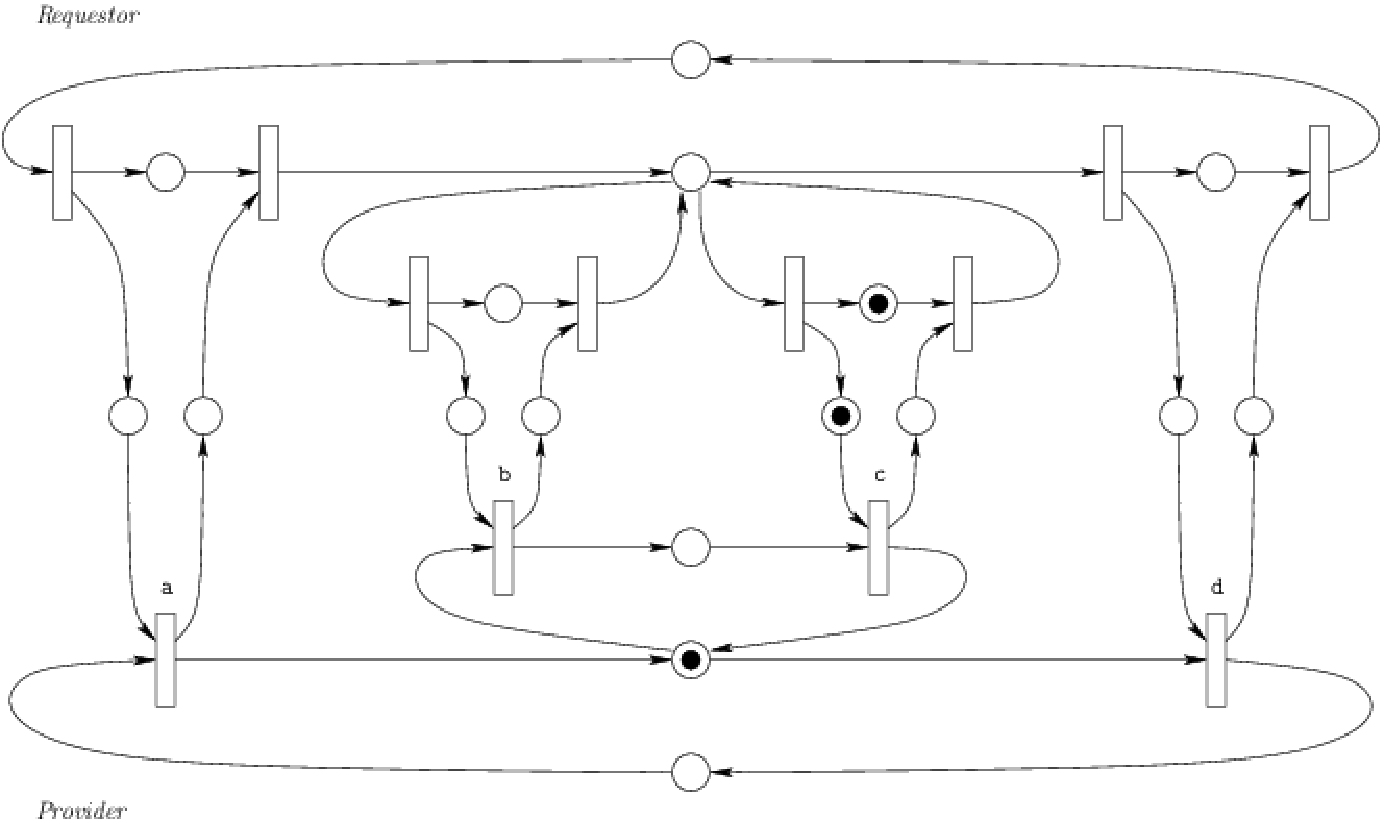
\includegraphics[scale=0.40]{Images/db-deadlock}
\caption{\label{fig:app-db-deadlock} Image of a deadlocked Petri net at 40\%
  scaling.} 
\end{figure}

\begin{table}[!htbp]
\centering
\caption{Fall Semester Enrollment}
\label{tab:app-pop}
\vspace{2mm}
\begin{tabular}{c||c|c|c||c|c|c|}
\hline
	& \multicolumn{3}{c||}{Undergraduate}
	& \multicolumn{3}{c|}{Graduate} \\
\cline{2-7}
     & F/T & P/T & Total & F/T & P/T & Total \\
\cline{2-7}
2004 & 13,191 & 2,223 & 15,414 & 1,308 & 879 & 2,187 \\
2005 & 13,184 & 2,143 & 15,327 & 1,375 & 920 & 2,295 \\
2006 & 12,809 & 2,224 & 15,033 & 1,373 & 899 & 2,272 \\
2007 & 12,634 & 2,155 & 14,789 & 1,403 & 899 & 2,302 \\
2008 & 12,269 & 2,208 & 14,477 & 1,410 &1,005& 2,415 \\
2009 & 12,382 & 2,323 & 14,705 & 1,567 &1,106& 2,673 \\
\hline
\end{tabular}
\end{table}

\section{Equations}
An example mathematical formulae is show in~\ref{eqn:appsum}.

\begin{equation}\label{eqn:appsum}
\sum_{i = 0}^{n} i^2
\end{equation}

% apdxb.tex

\chapter{Appendix: How to Add Another One}\label{apdx:b}

This is Appendix~\ref{apdx:b}.


\end{document}
